\documentclass[12pt, % The default document font size, options: 10pt, 11pt, 12pt
%oneside, % Two side (alternating margins) for binding by default, uncomment to switch to one side
%chapterinoneline,% Have the chapter title next to the number in one single line
english, % ngerman for German
singlespacing, % Single line spacing, alternatives: onehalfspacing or doublespacing
%draft, % Uncomment to enable draft mode (no pictures, no links, overfull hboxes indicated)
2%nolistspacing, % If the document is onehalfspacing or doublespacing, uncomment this to set spacing in lists to single
%liststotoc, % Uncomment to add the list of figures/tables/etc to the table of contents
%toctotoc, % Uncomment to add the main table of contents to the table of contents
%parskip, % Uncomment to add space between paragraphs
%nohyperref, % Uncomment to not load the hyperref package
headsepline, % Uncomment to get a line under the header
]{MastersDoctoralThesis} % The class file specifying the document structure


\graphicspath{ {images/} }

\providecommand{\tabularnewline}{\\}
\sloppy



\usepackage[utf8]{inputenc} % Required for inputting international characters
\usepackage[T1]{fontenc} % Output font encoding for international characters
\usepackage{graphicx}
\usepackage{aas_macros}
\usepackage{amsmath}
\usepackage{stackrel}
\usepackage{amssymb}
\usepackage{txfonts}
\usepackage[authoryear]{natbib}
\usepackage{multirow}
\usepackage{color}
\usepackage[colorlinks=true, citecolor=blue]{hyperref}
\usepackage{palatino} % Palatino font
\usepackage{tabto} 
\usepackage{url}
\usepackage{afterpage}
\usepackage{longtable}
\onehalfspacing

\hypersetup{linktocpage} % For linking the bookmarks to page numbers in Tables of Contents, Figures, Tables, Publications etc.
\hypersetup{colorlinks,linkcolor=blue}


\makeatletter
\setlength{\@fptop}{0pt}
\setlength{\@fpbot}{0pt plus 1fil}
\makeatother




\definecolor{checkcolor}{rgb}{0.75, 0.75, 0.75}
\newsavebox{\definitionbox}
\newenvironment{checkit}{
\begin{lrbox}{\definitionbox}
\begin{minipage}[t]{0.90\textwidth}
}
{\end{minipage}\end{lrbox}
\begin{center}{\colorbox{checkcolor}{\usebox{\definitionbox}}}
\end{center}}





\global\newcommand{\B}{BATSE}
\global\newcommand{\grb}{GRB151006A}
\global\newcommand{\s}{\emph{Swift}}
\global\newcommand{\f}{\emph{Fermi}}
\global\newcommand{\A}{\emph{Athena}}
\global\newcommand{\D}{\emph{Daksha}}
\global\newcommand{\C}{\emph{Chandra}}
\global\newcommand{\bs}{\emph{BeppoSax}}
\global\newcommand{\AS}{\emph{AstroSat}}
\global\newcommand{\X}{\emph{XMM-Newton}}

\global\newcommand{\ee}{E_0}
\global\newcommand{\dd}{{\rm d}}
\global\newcommand{\al}{allowable}
\global\newcommand{\Ep}{E_{\rm p}}
\global\newcommand{\Lp}{L_{\rm p}}
\global\newcommand{\fsc}{\alpha_f}
\global\newcommand{\keV}{\rm{keV}}
\global\newcommand{\LX}{L_{\rm X}}
\global\newcommand{\thr}{threshold}
\global\newcommand{\T}{T_{\rm{90}}}
\global\newcommand{\fB}{f_{\rm{B}}}
\global\newcommand{\Lb}{L_{\rm{b}}}
\global\newcommand{\Msun}{M_{\odot}}
\global\newcommand{\M}{M_{\rm{sum}}}
\global\newcommand{\eL}{\emph{Left}}
\global\newcommand{\eR}{\emph{Right}}
\global\newcommand{\ps}{{\rm s^{-1}}}
\global\newcommand{\py}{{\rm yr^{-1}}}
\global\newcommand{\gc}{gross\_cutoff}
\global\newcommand{\Lbn}{L_{\rm{b,0}}}
\global\newcommand{\Eps}{E_{{\rm p,0}}}
\global\newcommand{\N}{N_{\rm{points}}}
\global\newcommand{\Np}{N_{\rm{pairs}}}
\global\newcommand{\tl}{t_{{\rm look}}}
\global\newcommand{\mus}{{\rm \mu s}}
\global\newcommand{\Rdot}{\overset{.}{R}}
\global\newcommand{\Rcap}{\stackbin{.}{R}}
\global\newcommand{\red}{\chi_{{\rm red}}^{2}}
\global\newcommand{\pyG}{{\rm yr^{-1}Gpc^{-3}}}
\global\newcommand{\ergpersec}{\rm erg \, s^{-1}}
\global\newcommand{\csfr}{\overset{.}{\rho_{\star}}}
\global\newcommand{\phpercmsqpersec}{\rm ph \, cm^{-2} \, s^{-1}}
\global\newcommand{\ergpercmsqpersec}{\rm erg \, cm^{-2} \, s^{-1}}


\defcitealias{Kouveliotou_et_al.-1993-ApJ}{K93}
\defcitealias{Band_et_al.-1993-ApJ}{B93}
\defcitealias{Bouwens_et_al.-2015-ApJ}{B15}
\defcitealias{Yonetoku_et_al.-2004-ApJ}{Y04}
\defcitealias{Amaral-Rogers_et_al.-2017-MNRAS}{AR17}
\defcitealias{Tan_et_al.-2013-ApJL}{T13}
\defcitealias{Paul-2018-MNRAS--long}{P18a}
\defcitealias{Yonetoku_et_al.-2014-ApJ}{Y14}
\defcitealias{Ghirlanda_et_al.-2016-A&A}{G16}
\defcitealias{Tsutsui_et_al.-2013-MNRAS}{Ts13}
\defcitealias{Guetta_and_Piran-2005-A&A}{GP05}
\defcitealias{Guetta_and_Piran-2006-A&A}{GP06}
\defcitealias{D'Avanzo_et_al.-2014-MNRAS}{DA14}
\defcitealias{Coward_et_al.-2012-MNRAS}{C12}
\defcitealias{Segreto_et_al.-2003-A&A--INTEGRAL_cosmic_rays}{S03}
\defcitealias{Blandford_&_Konigl-1979-ApJ}{BK79}
\defcitealias{Beams_and_jets}{Cawthorne (1991)}
\defcitealias{Ziolkowski-2014-MNRAS}{Zi14}
\defcitealias{Stirling_et_al.-2001-MNRAS}{S01}
\defcitealias{Orosz_et_al.-2011-ApJ}{O11}
\defcitealias{Zdziarski-2012-MNRAS-Radio_modulation_CX1}{Zdziarski, 2012}
\defcitealias{Zdziarski_et_al.-2012-MNRAS-MeV_tail_CX1}{Z12}
\defcitealias{Heinz-2006-ApJ}{Heinz, 2006}
\defcitealias{Longair-3rd_Ed.}{Longair, 2011}
\defcitealias{Rybicki_&_Lightman}{Rybicki and Lightman (1979)}

\geometry{
	paper=a4paper, % Change to letterpaper for US letter
	inner=1.0in, % Inner margin
	outer=1.0in, % Outer margin
	bindingoffset=2cm, % Binding offset
	top=1.5cm, % Top margin
	bottom=1.5cm, % Bottom margin
	%showframe, % show how the type block is set on the page
}





%\sloppy
\begin{document}



\frontmatter
\pagestyle{plain}


\begin{titlepage}
\begin{center}
{\centerline {\bf {\Huge Gamma Ray Bursts in the \AS -CZTI era}}}
\vskip 2cm
{\centerline {\textsc{\Large A Thesis}}}
\vskip 2cm
{\centerline {\Large Submitted to the}}
\vskip 0.2cm
{\centerline {\Large Tata Institute of Fundamental Research, Mumbai}}
\vskip 0.2cm
{\centerline {\Large for the degree of Doctor of Philosophy}}
\vskip 0.2cm
{\centerline {\Large in Physics}}
\vskip 1.5cm
{\centerline {\Large by }}
\vskip .7cm
{\centerline {\textsc{\Large Debdutta Paul}}}
\vskip 2.5cm
{\centerline {\Large School of Natural Sciences}}
\vskip 0.2cm
{\centerline {\Large Tata Institute of Fundamental Research}}
\vskip 0.2cm
{\centerline {\Large Mumbai}}
\vskip 0.2cm
{\centerline {\Large May, 2019}}
\vskip 0.4cm
{\centerline {\Large Final version submitted in October, 2019}} %\textemdash, 2019}}
\end{center}
\end{titlepage}




\begin{declaration}
%\addchaptertocentry{\authorshipname}
\vskip 1cm
\noindent This thesis is a presentation of my original research work. Wherever contributions of others are involved, every effort is made to indicate this clearly, with due reference to the literature, and acknowledgement of collaborative research and discussions.\\
\noindent The work was done under the guidance of Professor A R Rao, at the Tata Institute of Fundamental Research, Mumbai.
\vskip 3cm
\begin{flushright}
\textbf{DEBDUTTA PAUL}
\end{flushright}
\begin{flushright}
%{\bf [Candidate's name and signature]}
\end{flushright}
\vskip 1.5cm
\noindent In my capacity as supervisor of the candidate's thesis, I certify that the above statements are true to the best of my knowledge.
\vskip 3cm
\begin{flushleft}
\textbf{Professor A R RAO}
\end{flushleft}
\begin{flushleft}
%{\bf [Guide's name and signature]}
\end{flushleft}
\vskip 0.5cm
\noindent Date:
\end{declaration}
\cleardoublepage



\begin{acknowledgements}
No amount of acknowledgement would be enough to express the gratitude I feel for you, Professor Rao. Your presence has not only helped me do scientific research, but has vastly shaped me as a person. My deepest regards to you are for not only being my Thesis supervisor to the truest of terms, but for performing duties well beyond the call of that; for being my best critic; and for being the prime example of someone you think worth becoming. I am one of those luckiest graduate students born on this planet.

I am deeply indebted to Professor Dipankar Bhattacharya, not only for excellent academic suggestions, advice, and support, but also for showing what diligence and effective communication can achieve; you are a master of many arts, achieving even a fraction of which is a lot for young researchers like me. Thank you for being such a massive inspiration.

I would like to express my deep gratitude to many people who have helped me at different stages of my TIFR journey: my batchmates Sounak and Sarbajaya for helping me survive graduate course work; my previous flatmates Gowtham and Aditya for being such nice human beings and friends in need; Joe Philip Ninan, for being a friend, an amazing senior, an excellent teacher of the tricks of the trade, and a source of great inspiration; senior Jishnu Bhattacharya for great advice as well as helping me with many technical details; Professor Rajdeep Sensarma for being an excellent teacher; Professors Rishi Sharma and Basudeb Dasgupta for guiding me at a crucial stage; and Professors D K Ojha and H M Antia for departmental support. This Thesis would not have been possible without either of you.

My sincere thanks to Professor Andrzej A Zdziarski for amazing scientific leadership, and warm hospitality at NCAC, Warsaw. I would like to thank all the members of the \AS -CZTI collaboration, but especially Rakesh Khanna, Mithun NPS, and Ajay Vibhute, for helping me integrate smoothly into the collaboration and with data and pipeline related queries throughout; and Vidushi Sharma for various updates about detected GRBs. My deepest gratitude is for all members of the staff of the TIFR canteens and Jagadish canteen, as well as the doctors and staff of the TIFR Medical Section, for their constant services that ensured an easy life in the campus.

I have deep regards for those who showed me the world of mountains, and those with whom I continue to share the love for this world -- a good fraction of these years has been spent in your lovely company. Naming you all is a mountain that I would rather not attempt to climb! I would like to thank my friends: Susmita for moral support during challenging times, and Jyotirmoy for being such a lovely person to be around with.

The last few months have been the toughest, but would have been worse without your timely intervention and excellent guidance: Nandini, I owe a lot to your hand of friendship, without which reaching the stage of completion would not have been a reality. I sincerely thank my psychotherapist Dr Priyanka Raut for digging me out of the pit that I was stuck in. I express my gratitude to Professor Sourav Chatterjee, for being a friend rather than a colleague: academia needs more people like you who takes mental health and depression seriously, and lends a hand of support during testing times.

None of the research I did would have been possible without the great works of the coders of the Free Software Foundation, to whom I express my most sincere gratitude. I would like to thank the Government of India and the people of this nation for funding my research.

Finally and most importantly, I express my sincere thanks to my parents, for believing in my dreams.
\end{acknowledgements}


\dedicatory{To Professor Asok Kumar Das, (retired, Scottish Church College, Kolkata), for showing me that beauty lies in truth, and happiness in objective thinking.}




\tableofcontents
\listoffigures
\listoftables

\begin{abbreviations}{ll} % A table of two columns
\textbf{Athena} & \textbf{A}davanced \textbf{T}elescope for \textbf{H}igh \textbf{E}nergy \textbf{A}strophysics\\
\textbf{BAT} & \textbf{B}urst \textbf{A}lert \textbf{T}elescope\\
\textbf{BATSE} & \textbf{B}urst \textbf{A}nd \textbf{T}ransient \textbf{S}ource \textbf{E}xperiment\\
\textbf{BH} & \textbf{B}lack \textbf{H}ole\\
\textbf{BNSM} & \textbf{B}inary \textbf{N}eutron \textbf{S}tar \textbf{M}erger\\
\textbf{BPL} & \textbf{B}roken \textbf{P}ower \textbf{L}aw\\
\textbf{CAM} & \textbf{C}oded \textbf{A}perture \textbf{M}ask\\
\textbf{CGRO} & \textbf{C}ompton \textbf{G}amma \textbf{R}ay \textbf{O}bservatory\\
\textbf{CSFR} & \textbf{C}osmic \textbf{S}tar \textbf{F}ormation \textbf{R}ate\\
\textbf{CPM} & \textbf{C}harged \textbf{P}article \textbf{M}onitor\\
\textbf{CZTI} & \textbf{C}admium \textbf{Z}inc \textbf{T}elluride \textbf{I}mager\\
\textbf{DDH} & \textbf{D}etector \textbf{D}elay \textbf{H}istogram\\
\textbf{DPH} & \textbf{D}etector \textbf{P}lane \textbf{H}istogram\\
\textbf{ECPL} & \textbf{E}xponential \textbf{C}utoff \textbf{P}ower \textbf{L}aw\\
\textbf{EM} & \textbf{E}lectro\textbf{m}agnetic\\
\textbf{FOV} & \textbf{F}ield \textbf{O}f \textbf{V}iew\\
\textbf{GBM} & \textbf{G}amma-ray \textbf{B}urst \textbf{M}onitor\\
\textbf{GRB} & \textbf{G}amma \textbf{R}ay \textbf{B}ursts\\
\textbf{GW} & \textbf{G}ravitational \textbf{W}aves\\
\textbf{INTEGRAL} & \textbf{Inte}rnational \textbf{G}amma-\textbf{R}ay \textbf{A}strophysics \textbf{L}aboratory\\
\textbf{IPN} & \textbf{I}nter-\textbf{P}lanetary \textbf{N}etwork\\
\textbf{KAGRA} & \textbf{KA}mioka \textbf{GRA}vitational-wave detector\\
\textbf{LAXPC} & \textbf{L}arge \textbf{A}rea \textbf{X}-ray \textbf{P}roportional \textbf{C}ounter\\
\textbf{LF} & \textbf{L}uminosity \textbf{F}unction\\
\textbf{LH} & \textbf{L}ivingston-\textbf{H}anford\\
\textbf{LHV} & \textbf{L}ivingston-\textbf{H}anford-\textbf{V}irgo\\
\textbf{LHVKI} & \textbf{L}ivingston-\textbf{H}anford-\textbf{V}irgo-\textbf{K}AGRA-\textbf{I}ndia\\
\textbf{LIGO} & \textbf{L}aser \textbf{I}nterferometer \textbf{G}ravitational-Wave \textbf{O}bservatory\\
\textbf{NS} & \textbf{N}eutron \textbf{S}tar\\
\textbf{PICsIT} & \textbf{Pi}xelated \textbf{C}e\textbf{s}ium \textbf{I}odide \textbf{T}elescope\\
\textbf{SAA} & \textbf{S}outh \textbf{A}tlantic \textbf{A}nomaly\\
\textbf{SED} & \textbf{S}pectral \textbf{E}nergy \textbf{D}istribution\\
\textbf{SNR} & \textbf{S}ignal-to-\textbf{N}oise \textbf{R}atio\\
\textbf{SPL} & \textbf{S}imple \textbf{P}ower \textbf{L}aw\\
\textbf{SXT} & \textbf{S}oft \textbf{X}-ray \textbf{T}elescope\\
\textbf{TDE} & \textbf{T}idal \textbf{D}isruption \textbf{E}vent\\
\textbf{UVIT} & \textbf{U}ltra-\textbf{V}iolet \textbf{I}maging \textbf{T}elescope\\
\textbf{UVOT} & \textbf{U}ltra-\textbf{V}iolet/\textbf{O}ptical \textbf{T}elescope\\
\textbf{WFI} & \textbf{W}ide \textbf{F}ield \textbf{I}mager\\
\textbf{XMM} & \textbf{X}-ray \textbf{M}ulitmirror \textbf{M}ission\\
\textbf{XRT} & \textbf{X}-\textbf{R}ay \textbf{T}elescope\\
\\
\textbf{aLIGO} & \textbf{a}dvanced \textbf{LIGO}\\
\textbf{LGRB} & \textbf{L}ong \textbf{GRB}\\
\textbf{SGRB} & \textbf{S}hort \textbf{GRB}\\
\end{abbreviations}



\chapter*{List of Publications}
\section*{Thesis related publications in refereed journals}


\begin{enumerate}

\item \textbf{Paul, D.}; 2018; MNRAS, 477, 4275; Binary neutron star merger rate via the luminosity function of short gamma-ray bursts.

\item \textbf{Paul, D.}; 2018; MNRAS, 473, 3385; Modelling the luminosity function of long gamma-ray bursts using \s\ and \f.

\item Rao et al.; 2016; ApJ, 833, 86; \AS\ CZT Imager Observations of GRB151006A: Timing, Spectroscopy, and Polarization Study.

\item Zdziarski, \textbf{Paul}, Osborne, Rao; 2016; MNRAS, 463, 1153; Anisotropy of partially self-absorbed jets and the jet of Cyg X-1.

\end{enumerate}



\section*{Thesis related publications under peer review}


\begin{enumerate}

\item \textbf{Paul} et al.; 2019; Experimental Astronomy; Detection and Characterisation of Cosmic Rays in \AS -CZTI data.

\end{enumerate}
\cleardoublepage






\mainmatter
\pagestyle{thesis}


\chapter{Introduction}
\label{chap:introduction}
\section{The enigma of Gamma Ray Bursts}
\label{sec:enigma}
Humans have long explored the universe beyond the `visible' wavelengths. From the low-frequency radio waves used to detect cosmic microwave background radiation, to the high-frequency ``hard'' X-rays and $\gamma$-rays\footnote{The distinction between ``soft'' and ``hard'' X-rays, as well as ``hard X-rays'' and ``$\gamma$-rays,'' is subjective, and loose. In this Thesis, photons of energies lower than $10$ keV will be referred to as ``soft X-rays,'' photons of energies between $10$ keV and $200$ keV will be referred to as ``hard X-rays,'' and those with higher energies will be referred to as ``$\gamma$-rays.''},  they have opened their eyes to observe the universe in all domains of the electromagnetic spectrum. Each new window has initially thrown up mysteries, clouding the vision until years of effort cleared it. Recently, we have opened up a set of `ears': gravitational waves [GWs].

Just as necessity has driven invention, war has pushed the frontiers of human knowledge to expedite discoveries otherwise unlikely, if not impossible. One such discovery is what we know today as `Gamma Ray Bursts' [GRBs]. In the height of the Cold War, the American `Vela' satellites, while playing vigil to possible violations of the Nuclear Test Ban Treaty by the erstwhile U.S.S.R, chanced upon a phenomenon that remained shrouded in mystery as classified government documents until its astrophysical nature was firmly established. Reported $5$ years since discovery \citep{Klebesadel_et_al.-1973-ApJL}, Gamma Ray Bursts remained an enigma for another two decades.

As the name suggests, GRBs are `bursts' of $\gamma$-rays: short-lived, transient phenomenon in the hard X-ray/$\gamma$-ray detectors, lasting from milliseconds to tens of seconds. $\gamma$-ray photons are absorbed by the Earth's atmosphere, hence making life possible, but requiring observation from above the atmosphere. On the other hand, these high-energy photons pass with ease through detector materials. This necessitates increasing the area of the detecting material to register more photons, compromising on the sky-localisation of the X-ray/$\gamma$-ray sources. This meant that the sky localisation of the bursts was very poor, covering hundreds of square degrees. Unable to tell whether these astrophysical sources originated in our own galaxy [the Milky Way] or not, plausible theories included everything above and beyond the earth, colliding neutron stars to giant flares on our Sun [see \cite{Nemiroff-1994-review} for a review].

In the years following the discovery, GRBs remained a mystery primarily due to the lack of association with other astrophysical objects. To do this, one required the sky location of the burst to follow up at other wavelengths, but that had to be done before the burst faded. Although the InterPlanetary Network [IPN] \citep{Cline_and_Desai-1976-Ap&SS} was set up in the 1970s and provided localisation of some bursts up to a few hundred square degrees, it was still a large part of the sky for ground-based optical/infrared telescopes to attempt a follow-up. Moreover, the delay from the detection to the localisation was much more than the burst time-scales, and hence they could not be followed up.

It was only in the 1990s when the $\gamma$-ray detector Burst And Transient Alert Telescope [\B] \citep{Fishman_et_al.-1989-BAAS} on-board the \emph{Compton Gamma Ray Observatory} [\emph{CGRO}] started detecting GRBs routinely, and localising them to degrees accuracy \citep{Briggs-1995-Ap&SS}, that their isotropic distribution on the sky was firmly established. Still the debate between extragalactic distances and sources distributed in the Milky Way halo, remained, urgently requiring an estimation of the distance. The Italian-Dutch satellite \bs\ \citep{Boella_et_al.-1997-A&AS} could follow up GRBs at higher wavelengths at a few hours' times-scales, and the redshift measurement of two GRBs by identifying the host galaxies, GRB970228 \citep{van_Paradijs_et_al.-1997-Nature} and GRB970508 \citep{Metzger_et_al.-1997-Nature}, firmly established that they were located at cosmological distances.

The cosmological locations of GRBs raised more questions than answers. Given their large distances, short durations, and the observed flux, their intrinsic luminosities [$\sim 10^{52} \, \ergpersec$] were orders of magnitude greater than any astrophysical object ever known: they outshine their entire parent galaxies in the short lifespan, the brightest supernova by around $10$ orders of magnitude, and even the more powerful distant quasars by at least $3$ orders of magnitudes. What powers them? The clue lay in the fact that not a single GRB was ever found to repeat, indicating that they were signatures of cataclysmic events, possibly violent deaths of massive stars. Given the finite speed of light, their short time-scales implied that the length-scales associated with them are much smaller than astronomical length-scales, indicating that they were associated with compact objects, like neutron stars [NSs] and black holes [BHs].


\section{What we know about GRBs}
\label{sec:what_we_know}
We have come a long way since the discovery of GRBs, and the age of the enigma of GRBs is over. Today, we can claim to understand GRBs as well as we understand BHs. Questions remain unanswered, but we are not hunting in the dark.

The quantity used to define the duration of a burst is called the $\T$, defined as the interval in which the central $90 \%$ of the flux is observed. Based on the observed distributions of $\T$\footnote{and `hardness', a measure of whether more photons were detected in a higher energy window, as compared to a lower energy window} of a sample of GRBs detected by \B, \cite{Kouveliotou_et_al.-1993-ApJ} [hereafter \citetalias{Kouveliotou_et_al.-1993-ApJ}] found that the sample can be divided into the so-called `long' and `short' bursts, $\T \lessgtr 2$ s. The observed event rate was found to be $\sim 150 \, \py$ on an average for `long GRBs' [LGRBs], and $\sim 10 \, \py$ for `short GRBs' [SGRBs], almost an order of magnitude smaller. Over the years, several lines of evidence suggested that the two classes are physically distinct classes, having different progenitors. Being associated with Type Ic supernovae \citep{Woosley_and_Bloom-2006-ARA&A} and also exclusively located at star forming regions within their galaxies \citep{Wainwright_et_al.-2007-ApJ, Fruchter_et_al.-2006-Nature}, LGRBs were conclusively associated with the death of massive stars collapsing directly into BHs, or perhaps into NSs \citep{MacFayden_and_Woosley-1999-ApJ, Woosley_and_MacFayden-1999-A&AS}. On the other hand, the lack of supernovae associations with SGRBs, their occurrence in older and elliptical galaxies, high offset from the host galaxy, etc. [see \cite{Berger-2014-sGRB_review} for a review] suggested that the SGRB progenitor is the merger of compact objects, like a pair of neutron stars [NSs], or a NS-BH, giving rise to relativistic jets \citep{Eichler_et_al.-1989-Nature, Narayan_et_al.-1992-ApJ} [also see \cite{Nakar-2007-PhR} for a review]. Recently, the detection of gravitational waves [GWs] from a binary neutron star merger [BNSM], GW170817 \citep{GW170817-2017}, along with its electromagnetic counterparts including the predicted `kilonova' \citep{EM170817-2017}, provided conclusive evidence of this association.

Irrespective of the differences of the progenitors, the `central engine', that is the source of energy that powers the transient emission is similar for the two classes of GRBs \citep{Ghirlanda_et_al.-2009-A&A, Calderone_et_al.-2015-MNRAS}: ultra-relativistic jets powered from the immediate environment of the nascent NS or BH [see \cite{Kumar_and_Zhang-2015-PhR} for a detailed review]. The Lorentz factors of these jets can be as high as $1000$ at the start of the prompt emission phases \citep{Abdo_et_al.-2009-Science}. The primary questions regarding GRBs can be posed in terms of questions regarding the launching and composition of the relativistic jets that give rise to the prompt emission. The physics of highly relativistic plasma in the presence of high magnetic fields, is however not extremely well-understood. Only recently has extensive computer simulations been catching up with the myriad details of non-thermal emission from ultra-relativistic matter originating very close to a nascent NS or BH, taking into account the effects of general relativity as well as three-dimensional hydrodynamics \citep{Sasha_et_al.-2008-MNRAS, Sasha_et_Al.-2010-NewA, Narayan_et_al.-2011-MNRAS}.

Observational distinction is made between the `prompt' emission phase, that is the short-lived X-ray/$\gamma$-ray emission, and the progressively longer time-scale emission observed at lower frequencies [or equivalently, lower energies] lasting for hours, even days to weeks in the radio wavelengths. This so-called `afterglow' emission was understood to be arising from the circumbust medium of the GRB progenitors: as the relativistic jets entrain the circumbust medium and drive shocks through it, they slow down, and the circumbust medium cools down at progressively lower frequencies at larger distances from the centre of the progenitor. The evidence of the `achromatic jet-break' \citep{Fruchter_et_al.-1999-ApJ, Kulkarni_et_al.-1999-Nature, Stanek_et_al.-1999-ApJ, Harrison_et_al.-1999-ApJ, Frail_et_al.-2001-ApJ} [also see \cite{Fong_et_al.-2012-ApJ}, \cite{Fong_et_al.-2015-ApJ} for a summary] that is, the sudden drop in flux during the afterglow, proved to the smoking-gun evidence that the jets are ultra-relativistic, the jet-break being a direct consequence of the relativistic Doppler beaming. The reader is referred to \cite{Kumar_and_Zhang-2015-PhR} for a recent, extremely detailed review of the observations and theory of afterglow emission.

Studying the afterglow emission tells us about the environment of the GRB progenitors, as well as the large-scale properties of the jet. On the other hand, the prompt emission arises from ultra-relativistic matter very close to the newly-formed NS or BH. Hence, a careful study of the timing, spectroscopy, and polarization of the unprocessed hard X-ray and $\gamma$-ray prompt emission offers an unique probe to the launching and composition of relativistic jets from regions very close to compact objects.

There are broadly two kinds of research done with GRBs. From the early days of observation, it was known that each GRB has a timing profile, called the ``lightcurves,'' different from all others. Just like snowflakes, each GRB is unique. The first kind of research attempts to answer generic questions of the physics of relativistic jets -- their launching, composition, energy-scales, etc. -- via detailed studies of individual GRBs. This requires not only detection of GRBs, but also following them up individually with higher wavelength pointing telescopes, which can facilitate the identification of the host-galaxy. This, in turn, can help in estimating the distance to the burst, offer insights into the GRB formation process via their positions within the host galaxies, and help us study the chemical properties of the burst environment. The identification of the host galaxy of the first binary neutron star merger event GW/EM 170817 \citep{GW170817-2017, EM170817-2017} showed the importance of being able to do this kind of research.

The second kind of research done tries to use the fact that GRBs are seen at very high distances in the universe due to the extremely high luminosities. For example, \cite{Cucchiara_et_al.-2011-ApJ} reported the detection of GRB090429B at a redshift of $9.4$, at $\sim 5\%$ of the age of the present age of the universe, the most distant GRB seen till date. Studying populations of GRBs can offer insights into the way GRBs have formed through cosmic time-scales, the evolution of galaxies, etc. Claims have been made to use GRBs as an addition to the cosmic distance ladder \citep{Tan_et_al.-2013-ApJL}. But as we shall see in this Thesis, research along these lines lets us make important contributions to the study of individual GRBs.



\section{GRBs and \AS-CZTI}
\label{sec:GRBs_and_AstroSat}
The current dedicated GRB monitors in space are \s\ \citep{Gehrels_et_al.-2004-ApJ} and \f\ \citep{FermiGBM-2009-ApJ}, launched in 2004 and 2008 respectively. \s\ observes only a tenth of the sky, and detects a GRB once in every $\sim 3$ days. Its triggering instrument is called the Burst Alert Telescope [BAT], which is sensitive to only the hard X-rays, from $15$ to $150$ keV. It uses an imaging technique with the help of the coded aperture mask [CAM] on-board BAT to localise the detected GRB within a small region of the sky and slew to this location within roughly a minute, providing even more precise localisation with its softer X-ray and ultraviolet detectors, which are then followed up by ground-based detectors to study the afterglow emission \citep{Barthelmy_et_al.-2005-SSRv-SwiftBAT, Band-2006-ApJ}. Living up to its name, it has increased the number of GRBs with afterglow observations. \f\ on the other hand is an open detector, virtually observing the full sky, and is also sensitive within a wide range of $8$ keV to $10$ MeV. It detects [on an average] one GRB per day, but can provide only rough localisation of the detected GRB, which is a large patch in the sky [about tens of square degrees]. Hence, unlike \s, it does not facilitate the detection of afterglows.

\AS\ is an Indian multi-wavelength satellite, simultaneously observing a wide range of the electromagnetic spectrum: from optical/ultraviolet to hard X-rays/$\gamma$-rays \citep{Rao_et_al.-2016-arXiv-Astrosat}. It has four instruments on-board: Ultra-Violet Imaging Telescope [UVIT] \citep{Subramaniam_et_al.-2016-SPIE, Tandon_et_al.-2017-AJ, Tandon_et_al.-2017-JApA, Rahna_et_al.-2017-MNRAS}, Soft X-ray Telescope [SXT] \citep{Singh_et_al.-2016-SPIE, Singh_et_al.-2017-JApA}, Large Area X-ray Proportional Counter [LAXPC] \citep{Agrawal_et_al.-2017-JApA, Antia_et_al.-2017-ApJS, Yadav_et_al.-2017-arXiv}, and Cadmium Zinc Telluride Imager [CZTI] \citep{Bhalerao_et_al.-2017-JApA}. CZTI is a hard X-ray detector sensitive in the energy range $20$-$400$ keV, consisting of an array of CdZnTe crystals. Each detector module consists of $256$ independent detectors, called `pixels,' of size $2.5$ mm $\times \; 2.5$ mm each. The detector plane consists of four quadrants, each with $16$ detector modules, comprising an effective area of $1024 \, \rm{cm{^2}}$. CZTI has imaging capabilities below $100$ keV, using the Coded Aperture Mask [CAM] placed above collimator slats that surround the detector modules. The collimator is made of Tantalum of size $4$ cm $\times$ $4$ cm, which allows for a field of view [FOV] of $4.6^{\circ} \times 4.6^{\circ}$.

\begin{figure}
\begin{center}
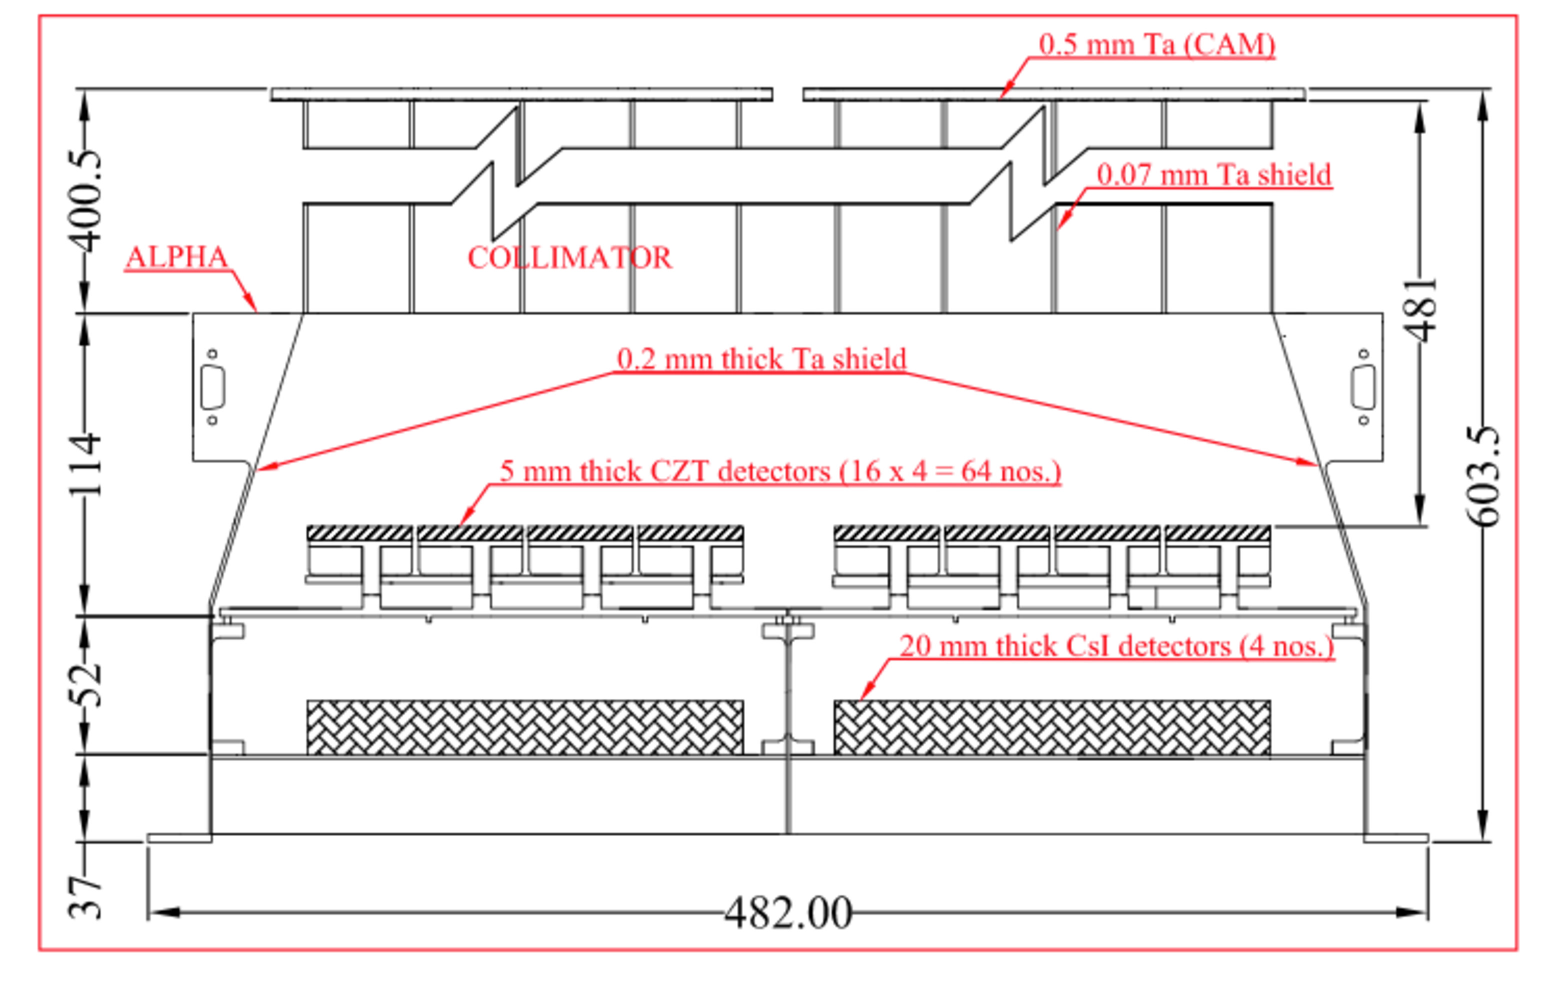
\includegraphics[scale=0.33]{GRB151006A--CZT}
\caption[Schematic diagram of \AS -CZTI]{A schematic diagram of the CZT instrument on the \AS\ satellite. All dimensions are in millimeters. A Tantalum coded aperture mask [CAM] at the top is backed by $400$ mm Al/Ta collimators, which restrict the view to $4.6^{\circ} \times 4.6^{\circ}$. Four identical quadrants with arrays of thick CZT modules forms the focal plane, $481$ mm below the CAM. The $2.46$ mm pixels matched to the CAM pitch provide a native angular resolution of $\sim 17^{'}$ in the primary field of view. $20$ mm thick CsI(Tl) scintillators mounted $\sim 66$ mm below the CZT modules provide active anti-coincidence shielding, and also function as a wide-angle detector in the $100$-$500$ keV range. This figure has been adopted from \cite{Rao_et_al.-2016-ApJ}.}
\label{fig:CZTI}
\end{center}
\end{figure}

After \AS\ was launched on the 28\textsuperscript{th} September, 2015, CZTI was the first payload to start observing astrophysical sources, on the 6\textsuperscript{th} October, 2015. On the very same day, it detected a long duration Gamma Ray Burst [GRB]: GRB151006A, which was also detected by \s\ and \f\ [the nomenclature refers to the date of detection by the \s\ satellite]. \s\ provided accurate sky-localisation, and \f\ provided a wide-band spectrum. This was the golden opportunity to calibrate \AS -CZTI. Using this GRB, it was shown in \cite{Rao_et_al.-2016-ApJ} that CZTI has capabilities of: (1) accurate timing studies of sources via time-tagged photon data every $20 \, \mus$; (2) spectroscopy in the wide range of hard X-rays via channel-to-energy conversion of the individual photons; (3) polarization studies of bright sources via the informations of detector-position and energy of coincident photons; and (4) few degrees localisation of transients detected off-axis, detailed in Chapter \ref{chap:localisation}.

Complementing the capabilities of the softer energy mission \s\ [$15$-$150$ keV] which has an unique capability of following up GRBs in real-time, and the harder energy mission \f\ [$8$ keV-$10$ MeV] which can accurately study the evolution of the spectra of the GRBs, CZTI was seen to possess the exciting capabilities of studying the unprocessed X-ray emission from GRBs at energy-range in-between \s\ and \f, as well as provide additional polarisation constraints. \cite{Basak_et_al.-2017-MNRAS} used the combined capabilities of \AS -CZTI along with the \s\ and \f\ data for this GRB to infer the re-injection of energy in the jet at $\sim 16$-$20$ s from the start of the prompt emission, even though the pulse profile was smooth throughout its activity.

\AS -CZTI has continued to play a crucial role in the study of GRBs ever since its inception. \cite{Chand_et_al.-2018-ApJ} reported high polarization from GRB 160802A, and used CZTI's capability of simultaneous temporal,  spectral, and polarimetric studies to infer about the emission mechanism of this GRB, as well as the properties of its jet. \cite{Chattopadhyay_et_al.-2017-arXiv} reported polarisation from $11$ GRBs in the first year of \AS 's operation. This significantly increased the number of GRBs with polarisation measurements, which can be used to constrain the emission mechanism of GRBs in general. \cite{Bhalerao_et_al.-2017-ApJ-A_Tale_of_Two_Transients} investigated whether the gravitational wave [GW] source GW170104 \citep{GW170104-2017}, a BH-BH binary, was associated with any electromagnetic counterpart. They reported the non-detection of any electromagnetic transient, and concluded that the GRB170105A detected by \AS -CZTI but not by \s\ or \f,  happened to be more than $20$ hours after GW170104, and was just a regular long GRB. Upon the first detection of an electromagnetic counterpart to a GW source GW170817 \citep{GW170817-2017, EM170817-2017}, \AS -CZTI played a crucial role via its non-detection of GRB170817A, detected by \f: It was understood that this source was in the Earth's shadow of CZTI, otherwise it would be detected with a signal-to-noise [SNR] of $> 10$, which information was used to rule out a large part of the sky for the localisation of this source \citep{Kasliwal_et_al.-2017-Science}.

\section{Scope of this Thesis}
\label{sec:scope}
In view of exciting studies of Gamma Ray Bursts using \AS -CZTI, one question becomes important to answer: What is the number of GRBs that \AS -CZTI can detect in a given time? The answer depends both on the instrumental characteristics of \AS -CZTI, as well as the intrinsic population of both long and short GRBs. There exists a true all-sky rate of GRBs, accounting for their cosmological rate of formation. A GRB detector samples from this superset, depending on its characteristics: solid angle of observation, average run time, the energy-band at which it observes, its flux-limit [also referred to as the `sensitivity'], etc. Hence, if the true cosmological and intrinsic distribution of GRBs can be theoretically constructed, one should be able to recover the rate of GRB detections by any X-ray/$\gamma$-ray detector, by specifying the detector's characteristics. As a by-product, one would also be able to study the intrinsic properties of the populations of both long and short bursts. With firm empirical evidence of the association of BNSMs and SGRBs, one may similarly ask: What is the rate of BNSMs that the current and future GW detectors are likely to detect? The answer lies in a careful study of the population of SGRBs.

Consider the following situation: There exists a population of torches at different distances from the observer. If all the torches had the same luminosity, then all torches up to a certain distance would be observed, whereas others at distances higher than that would not be. This limiting distance would be defined by the flux-limit of the observing instrument. But what if the torches had different luminosities? Then this intrinsic distribution over the parameter space of the torches' luminosities, written as $L$, would have to be taken into account to predict the number of torches we could observe with the same instrument. So is the case with GRBs and GRB detectors in space. The `luminosity function' [LF] is a probabilistic distribution function over the luminosity of the entire population of GRBs, denoted by $\Phi (L)$. To calculate the expected GRB-detection rate of \AS, it becomes necessary to construct this detector-independent quantity, separately for long and short GRBs. This Thesis reports the most updated constraints on the luminosity function of the long GRBs in Chapter \ref{chap:LGRBs}, and short GRBs in Chapter \ref{chap:SGRBs}. These are then used to predict the detection-rate of LGRBs and SGRBs for \AS -CZTI, as well as other future X-ray/$\gamma$-ray missions. These predictions are topical, and helps plan mission operations well in advance, as demonstrated in both these chapters.

Upon tallying the number of GRBs that \AS -CZTI actually detects versus the numbers predicted, it is noticed that a significant fraction of GRBs is missing. In Chapter \ref{chap:noise}, the reason behind this is carefully highlighted, via a re-investigation of the data analysis pipeline currently in place. Previously unreported in the CZTI data, high energy cosmic rays are detected. It is shown that the presence of this component in the data increases the number of false-positives of possible transients, to eliminate which, a significant number of GRBs are missed. A novel approach to solve this problem is proposed, and is currently being integrated in the CZTI data-analysis pipeline.

GRB photons are known to be powered by relativistic particles in large-scale collimated jets, via non-thermal mechanisms like synchrotron emission. The angular dependence of the non-thermal emission plays an important role in how the true cosmological population of GRBs is observed by an earth-based detector [Chapters \ref{chap:LGRBs} and \ref{chap:SGRBs}]. Hence, it is important to theoretically predict the angular dependence of synchrotron emission from relativistic jets. In Chapter \ref{chap:jet_model}, this was carried out in the more simple quasi-static regime, that is, when the particle distribution in the jet is quasi-statically maintained by the central engine. The formulae derived can be extended to GRBs by keeping the parameters of the model functions of time. The time-scale of evolution of these parameters will then be the time-scale of energy-injection by the central engine. The full-scale application of this idea is the scope of future work.

No scientific venture is ever complete: as one question is answered, new questions emerge. As an extension of comparing the durations of GRBs detected both by \s\ and by \f\ carried out in Chapter \ref{chap:LGRBs}, a careful re-investigation of this common catalogue of GRBs revealed a significant discrepancy of the durations of a small subset of bursts. To figure out the reason, each of these GRBs are being currently studied, and the preliminary idea and directed efforts are briefly summarised in Chapter \ref{chap:ongoing}. Finally, concluding remarks are presented in Chapter \ref{chap:conclusions}.

All the codes contributing to this Thesis were written in the free programming language, \textsc{python}, using freely available standard libraries. In line with the idea of open research, the codes have been made publicly available except to avoid conflicts with collaboration protocols.

\chapter[Localisation of off-axis CZTI GRBs]{Localisation of off-axis Gamma Ray Bursts with \AS-CZTI}
\label{chap:localisation}
\begin{checkit}
This work is based on \cite{Rao_et_al.-2016-ApJ}, and was carried out in collaboration with the other members of the \AS -CZTI group, to whom I express my sincere thanks, especially to Mithun NPS of the Physical Research Laboratory [PRL], Ahmedabad, India. It heavily relied on the inputs of two of the members, Professor Dipankar Bhattacharya of the Inter-University Centre for Astronomy and Astrophysics [IUCAA], Pune, India; and Vikas Chand, erstwhile graduate student of TIFR, Mumbai, India.
\end{checkit}


\section{Introduction}
\label{sec:introduction--localisation}
The Cadmium Zinc Telluride Imager [CZTI] on-board \AS\ uses an array of pixelated detectors and an equal area and equal size Coded Aperture Mask [CAM] for studying objects in the narrow field of view [FOV] of $4.6^{\circ} \times 4.6^{\circ}$ \citep{Bhalerao_et_al.-2017-JApA}. Being a virtually open detector at energies $> 50$ keV, CZTI does have the possibility of detecting transient events lying outside this narrow FOV. That is exactly what happened with the detection of GRB151006A on the very first day of its operation. This GRB was incident from $\sim 60^{\circ}$ from its pointing axis, as deduced from the \s -BAT sky-localisation of this burst. However, for GRBs incident at such large angles to its pointing axis, the CAM is ineffective. The question arose: Can CZTI independently localise such ``off-axis'' bursts  without the help of the CAM? If so, then the sample of GRBs that would be detected only by CZTI could be followed up in real time at smaller frequencies, enabling detection of their optical/radio afterglows.

\section{Localisation of \grb}
\label{sec:localisation--body}


\begin{figure}
\begin{center}
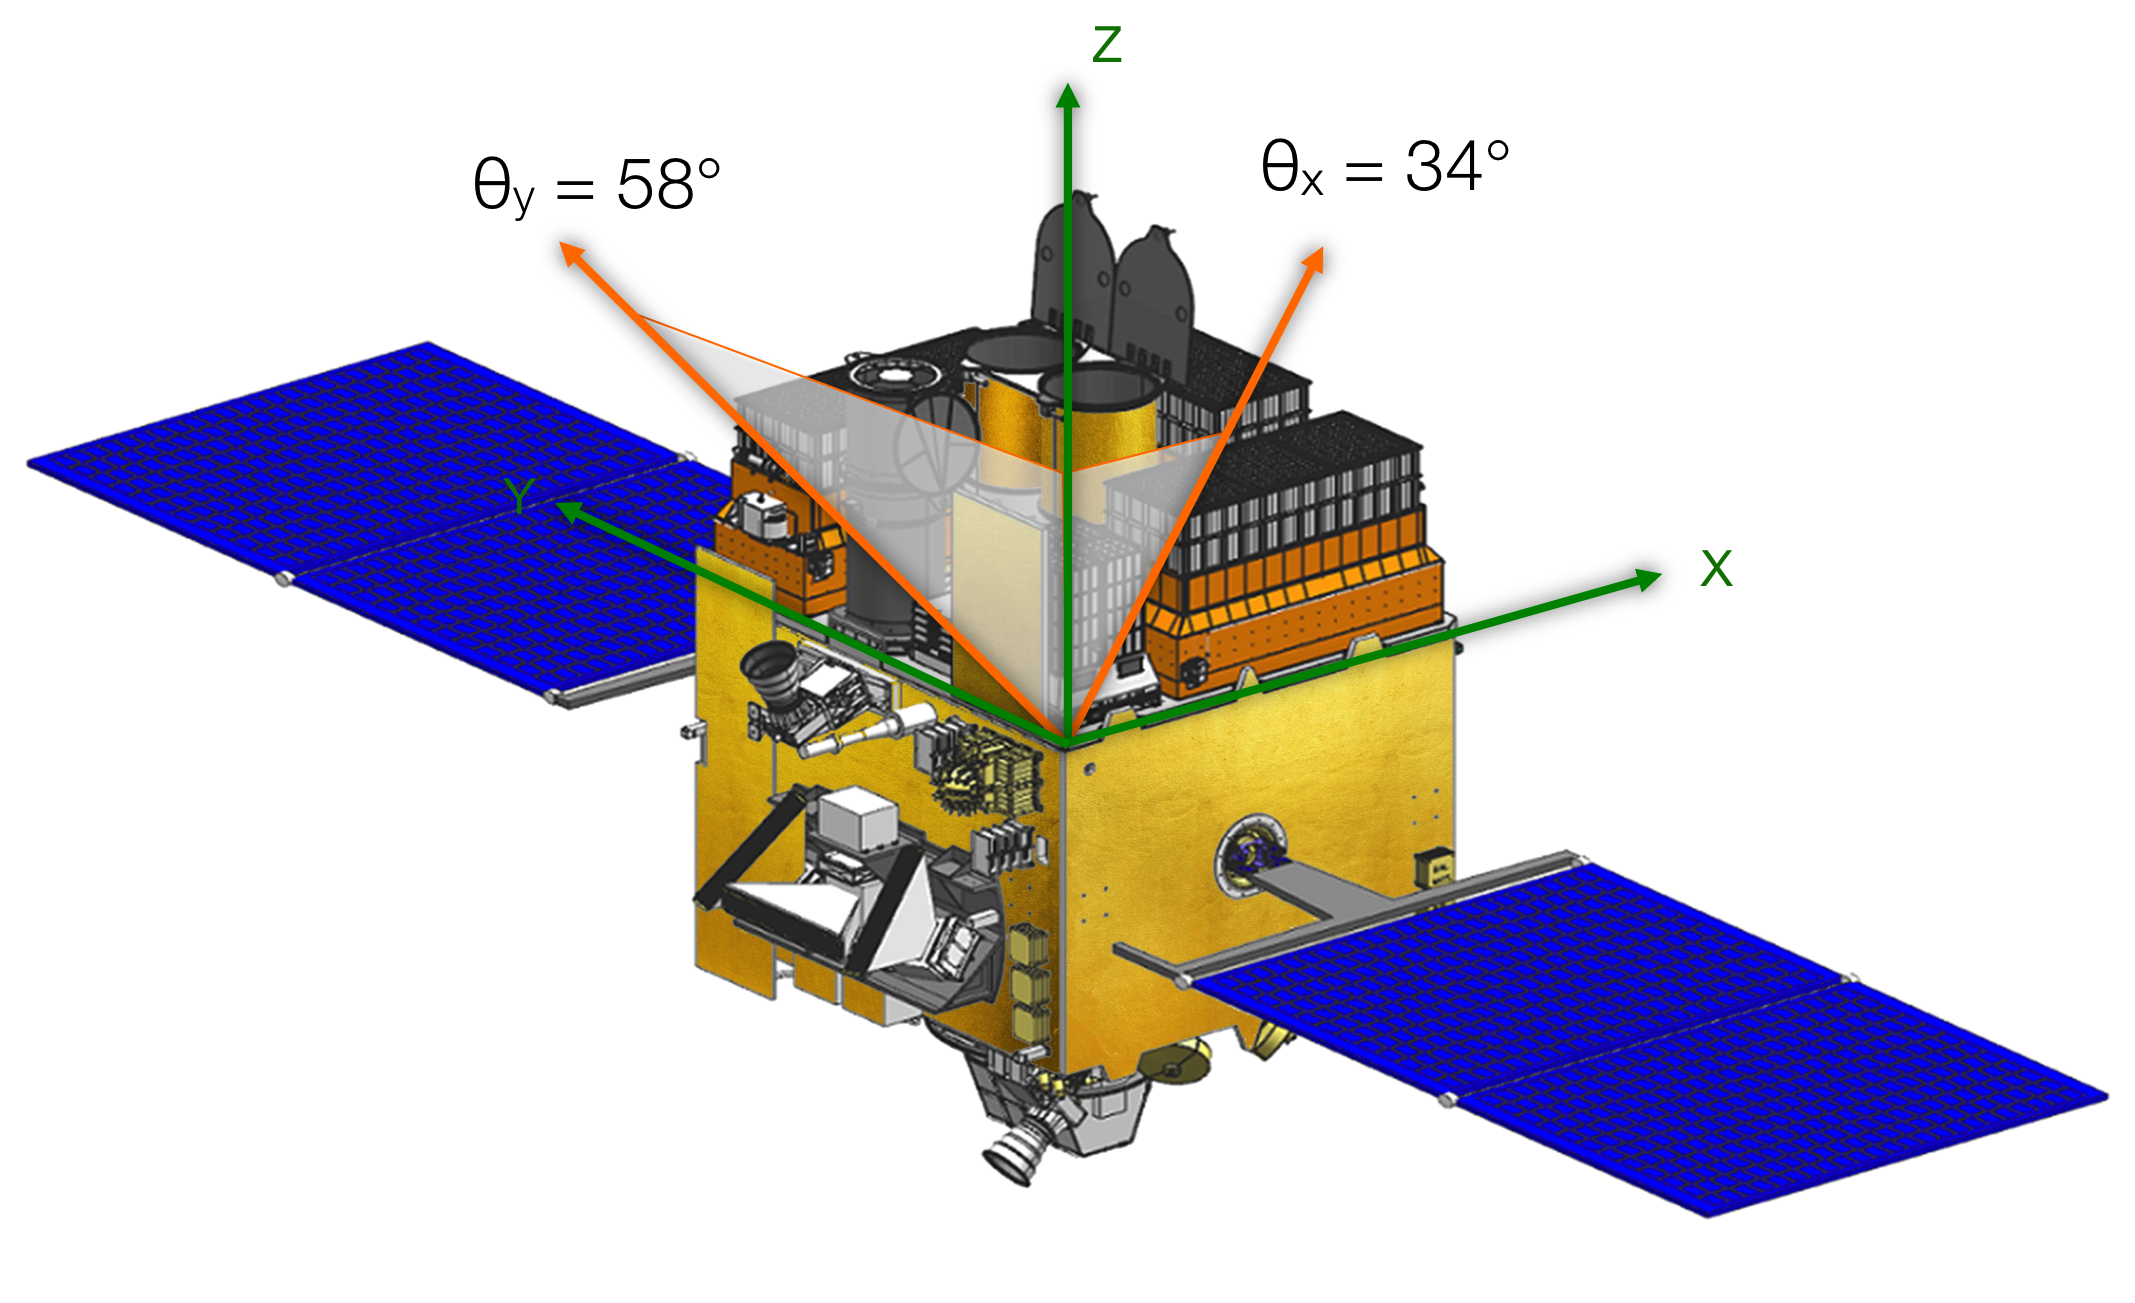
\includegraphics[scale=0.33]{GRB151006A--AstroSat}
\caption[Schematic diagram of the \s\ position of \grb\ with respect to local CZTI co-ordinates]{A schematic picture of \AS\ showing the relative positions of the different instruments, with respect to CZTI. The local coordinate systems of CZTI are defined. The angles $\theta_x$ and $\theta_y$ are measured [in degrees] from the Z-axis in the ZX and ZY planes respectively. The two components of the incident direction of \grb, assuming the sky-position given by \s, are indicated in terms of these angles. This figure has been adopted from \cite{Rao_et_al.-2016-ApJ}.}
\label{fig:GRB151006A--Swift_position}
\end{center}
\end{figure}


In this work, we explored the possibility of using the reasonably accurate position information for individual photons at the detector plane, coupled with the knowledge of mass distribution around the detectors, to localise transient events occurring outside the FOV of CZTI.

Professor Dipankar Bhattacharya [IUCAA, Pune] developed a ray tracing code in the \textsc{fortran} programming language to estimate the effective area of each pixel in the detector plane for an object at a given location in the sky. The mechanical structure given in Figure \ref{fig:CZTI} is represented by $63$ distinct surfaces which are converted into as many cuboids defined by area, thickness, absorbing material, and orientation with respect to the detector surface. For each pixel, the efficiency of transmission through all this material is calculated, along with the detection efficiency of the pixel and geometric projection terms, to give an effective area for a given source direction and energy, for each of the $2^{14} = 16384$ CZTI pixels.

Vikas Chand [erstwhile TIFR, Mumbai] used this off-axis spectral response to generate the spectrum for this GRB for the entire duration of its emission, $\sim 90$ s. The background subtraction was done using pre-burst and post-burst intervals of $90$ s and $200$ s respectively. He then obtained the best-fit parameters of the Band model \citep{Band_et_al.-1993-ApJ}, which fit the spectrum reasonably well.

\begin{figure}
\begin{center}
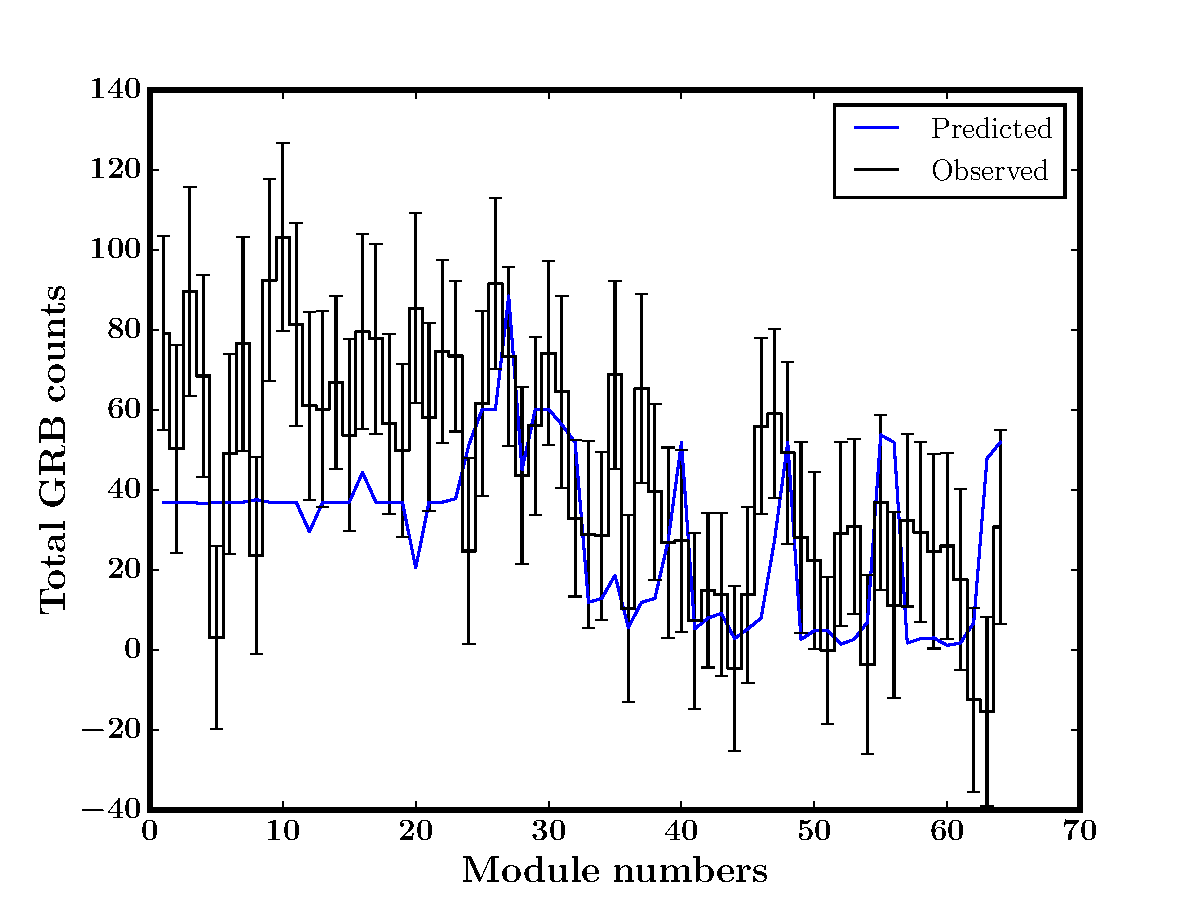
\includegraphics[scale=0.46]{GRB151006A--comparison}
\caption[Comparison between predicted and observed counts of \grb\ versus CZTI modules]{The predicted and observed counts for \grb, corresponding to the $64$ modules, indexed from $0$ to $63$ [according to CZT conventions], for the \s\ position of this GRB [see Figure \ref{fig:GRB151006A--Swift_position}]. The errors on the observed counts assumes statistical [Poisson] errors. Each of the modules is blocked by the instrument materials in a different way, and this is modelled by the ray-tracing code. An overall agreement is seen between the two curves.}
\label{fig:GRB151006A--comparison}
\end{center}
\end{figure}

Using the ray-tracing code, I calculated the pixel-wise efficiency for energies in steps of $5$ keV, for any given angle, expressed in local co-ordinates $\{ \theta_x$, $\theta_y \}$, see Figure \ref{fig:GRB151006A--Swift_position}. This information was then convolved with the spectral model fit to predict the pixel-wise efficiency for this GRB. Since the information in $2^{14}$ pixels is too large and hence the information in each pixel limited below the thresholds of Poisson statistics, the efficiency of all the pixels of a given module were summed, assuming that these pixels are independent of each other. This gave the module-wise counts for any given input angle $\{ \theta_x$, $\theta_y \}$, called the `predicted' counts for that angle.

The `observed' counts in each CZT Module [$64$ in number, indexed from $0$ to $63$ according to CZTI conventions] refers to the number of photons registered in that module for the same time-interval used in the spectral analysis, obtained from the data for this particular GRB, as well as the same pre- and post- burst intervals were chosen to do the background subtraction. A comparison of the predicted and observed counts for the \s\ position of this GRB [see Figure \ref{fig:GRB151006A--Swift_position}] is shown in Figure \ref{fig:GRB151006A--comparison}, and a reasonable agreement is seen.

\begin{figure}
\begin{center}
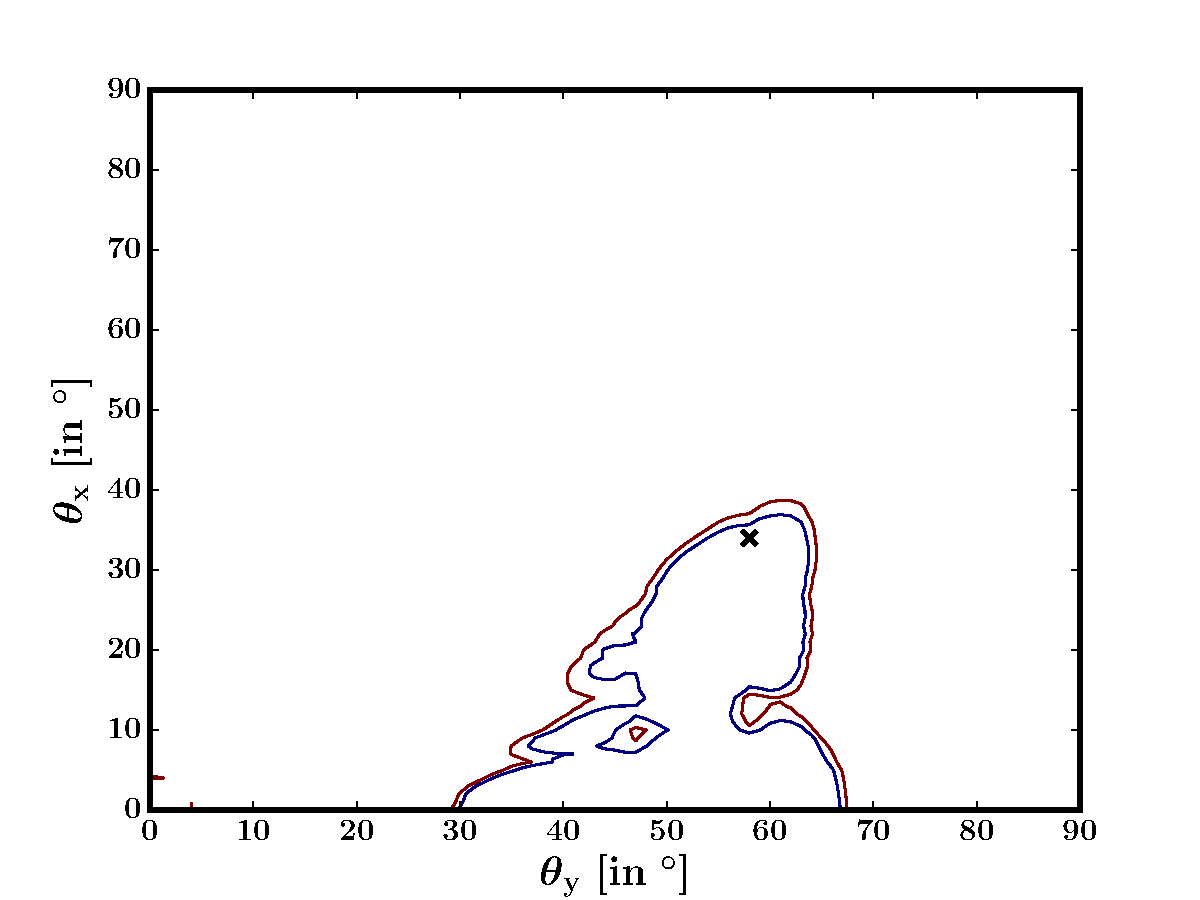
\includegraphics[scale=0.34]{GRB151006A--contours}
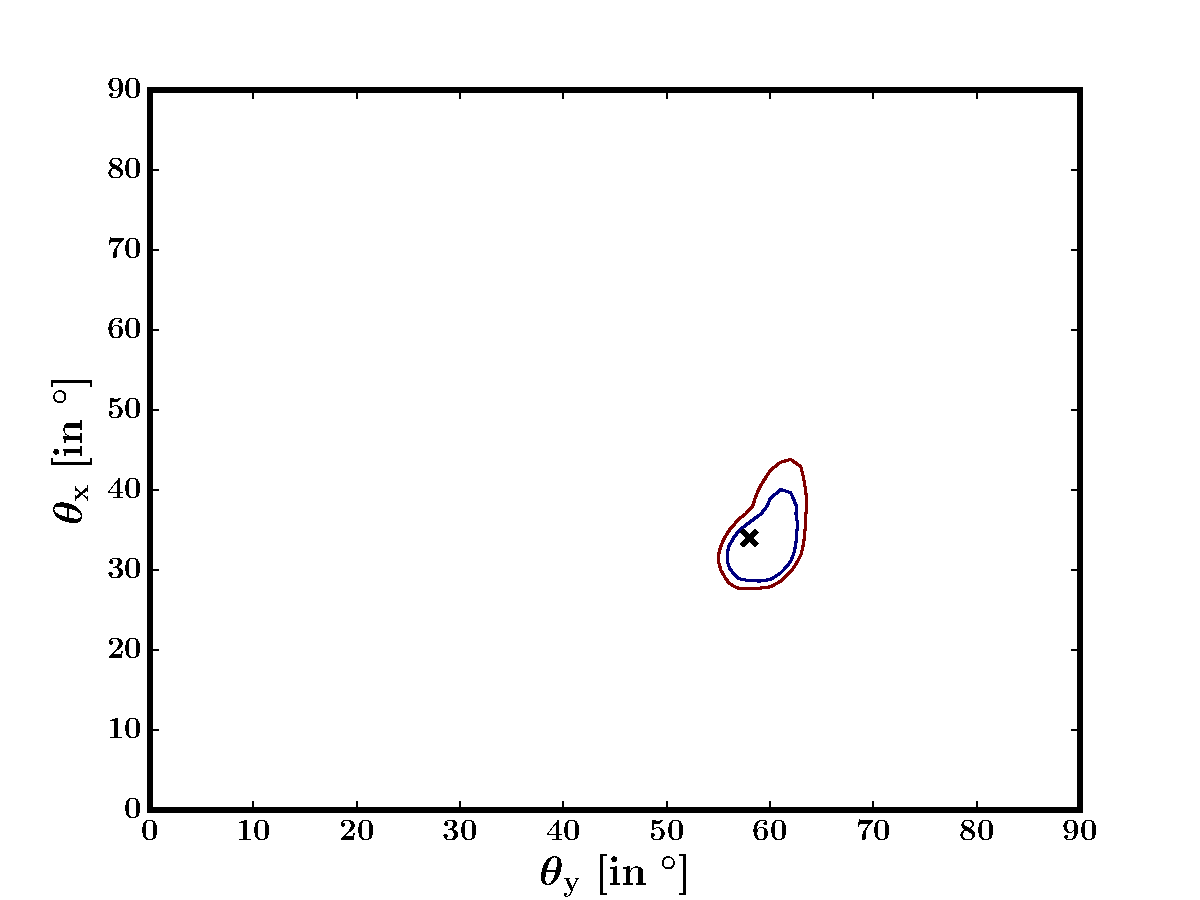
\includegraphics[scale=0.34]{GRB151006A--contours_sim}
\caption[Localisation capabilities of \AS -CZTI: theory and practice]{\eL: Contour plot of the $\chi^2$ between the observed and predicted counts, assuming statistical [Gaussian] errors. The predicted counts are generated for various incident angles, given in the local co-ordinates. The position of \grb\ is marked with a [black-] cross. The blue and brown $\chi^2$ contours correspond to $90 \%$ and $99 \%$ confidence levels, respectively. \eR: The $\chi^2$ contours [colours corresponding to same confidence levels] for a simulated burst of the same fluence, with $1 \sigma$ statistical [Poisson] errors added by hand. Comparison with the contours obtained from the data [left] implies that the assumption of statistical errors on the data is either incorrect or incomplete or both. That is, there is uncharacterised, systematic errors in the data.}
\label{fig:GRB151006A--contours}
\end{center}
\end{figure}

To test the localisation capabilities of CZTI, I simulated the instrument response in a grid of $\{ \theta_x$, $\theta_y \}$ coordinates, in units of $1^{\circ}$ in both $\theta_x$ and $\theta_y$, and convolved it with the spectral fit obtained for this GRB. On comparison with the observed values, the $\chi^2$ as a function of local $\{ \theta_x$, $\theta_y \}$ coordinates was obtained, shown in Figure \ref{fig:GRB151006A--contours}, \eL. It is seen that CZTI could have localised this GRB with an uncertainty of $\sim 10^{\circ}$.

In order to estimate the contribution of statistical errors to the data, I repeated the exercise by comparing simulated detector-wise counts for the $\{ \theta_x$, $\theta_y \}$ grid, with simulated counts for the true location of \grb\ [see Figure \ref{fig:GRB151006A--Swift_position}] and $1 \sigma$ statistical [Poisson] errors added by hand. The confidence contours obtained from this exercise are given in Figure \ref{fig:GRB151006A--contours}, \eR. It is seen that CZTI can localise GRBs of a fluence equal to that of \grb\ with an accuracy of a few degrees, and hence brighter GRBs to even sub-degrees accuracy.

The difference between this idealised case and real data may arise from three primary effects: (a) non-Poissonian errors in the data due to Cosmic Ray interactions; (b) effect of scattering in the detector material; and (c) effects of un-modelled absorption in other parts of the spacecraft. Amongst these, (b) and (c) can be tackled by generating a full mass-model of the entire \AS\ satellite. This means including all the components of the satellite and the relevant masses and the scattering surfaces, and simulating the transmission through as well as scattering from these surfaces. This project was implemented for other GRBs by using the \textsc{geant-4} software \citep{Bhalerao_et_al.-2017-ApJ-A_Tale_of_Two_Transients}, and is currently being integrated into the localisation scheme by new members of the CZTI collaboration. On the other hand, (a) was later studied by myself, and will be extensively discussed in Chapter \ref{chap:noise}.

\section{Conclusions}
\label{sec:conlusions--localisation}
With the first-day detection of \grb, it was demonstrated that \AS -CZTI is capable of detecting GRBs independent of other space-based X-ray missions. The various prospects of GRB science with CZTI were investigated with the help of this GRB, by comparing the capabilities of the instrument with well calibrated and understood GRB-detectors \s\ and \f. This GRB was outside the main field of view of the instrument, but still it was possible to study it in sufficient detail. The spectral properties of this GRB could be constrained by generating off-axis spectral response. This was done by tracing the photons paths through all the CZTI surfaces. Using the same ray-tracing algorithm, and the spectral fits, it was demonstrated that CZTI is capable of localising \grb\ up to tens of square degrees. Mock data generated from simulations showed that the same GRB should have been localised up to a few degrees if the noise in the data was indeed statistical. The results of a careful investigation of the noise in CZTI data are detailed in Chapter \ref{chap:noise}. Other reasons for the discrepancy could be unaccounted scattering in the CZTI surfaces, or scattering from other payloads on-board \AS. The polarisation of \grb\ was difficult to constrain due to its low fluence.
	
\chapter{Luminosity function of long GRBs}
\label{chap:LGRBs}
\begin{checkit}
This work is based on \cite{Paul-2018-MNRAS--long}. I sincerely thank Eric Burns for extremely helpful discussions about setting up the common catalogue of \s\ and \f\ GRBs; Professor A R Rao for helpful discussions and suggestions during the entire course of the work; \AS -CZTI member Vidushi Sharma for the updated list of GRBs detected by CZTI and related discussions; Professor Pawan Kumar for his comments on the manuscript of the paper; and the referee for the critical comments which immensely improved the quality of the work.
\end{checkit}



\section{Introduction}
\label{sec:introduction--LGRBs}
For any GRB detector, an interesting estimable quantity is the number of GRBs observed, as a function of measurable parameters. This depends on instrumental parameters like duration-of-operation $T$, and field-of-view $\Delta \Omega$, as well as the observed GRB production-rate and the distribution over intrinsic properties of GRBs. Let us assume that the rate of GRBs beamed towards an observer on earth from an infinitesimal co-moving volume $\dd V$, is given by $\Rdot (z) \frac{\dd V}{1+z}$, where $z$ denotes the redshift, and the factor $(1+z)^{-1}$ takes care of the cosmological time dilation.

Most generally, the number of GRBs detected by the instrument in the luminosity [$L$] range $L_1$ to $L_2$ and redshift range $z_1$ to $z_2$ is given by,

\begin{equation}
N(L_1,L_2; z_1,z_2) = T \, \dfrac{\Delta \Omega}{4 \pi} \, \intop_{max[L_1, \, L_c]}^{L_2} \Phi_z(L) \dd L \, \intop_{z_1}^{z_2} \dfrac{ \Rdot(z) }{1+z} \dd V,
\label{eq:definition_of_phi}
\end{equation} where $L_c$ denotes a lower-cutoff in the intrinsic luminosity of GRBs [see Section \ref{sec:The_estimated_luminosities--long}]. The function $\Phi_z(L)$ is formally called the `luminosity function' [henceforth LF], having the units of $(\ergpersec)^{-1}$, the subscript referring to an implicit dependence on the redshift. In view of the fact that GRBs are end-products of massive stars in galaxies, the GRB formation rate $\Rdot(z)$ can be written as
\begin{equation}
\Rdot(z) = \fB C\, \csfr,
\label{eq:R_dot--long}
\end{equation} where $\csfr$ gives the cosmic star formation rate [CSFR] in $ \pyG$, $C$ gives the efficiency of GRB production given a certain stellar mass, in units of $\Msun^{-1}$, and $\fB$ encodes the beaming effect of the relativistic jets producing the burst. All of these terms may be functions of the redshift.

The dependence of the detected number distribution of a certain class of astrophysical object on its luminosity function, is quite general. It has been extensively studied in the context of galaxies, galaxy clusters [see \cite{Galaxy_cluster_LF-2017-MNRAS} and references therein], white dwarfs [see \cite{White_dwarf_LF-2016-review} for a recent review], quasars [see \cite{Quasar_LF_in_UV-2017-MNRAS} and references therein], high mass Xray binaries [see \cite{High_mass_XRB_LF-2017-MNRAS} and references therein] etc. The methodologies depend on the observational window available for the study of the particular objects of interest [for example, while \cite{Galaxy_LF_using_WISE-2017-AJ}, \cite{Galaxy_LF_in_Kband-2017-MNRAS}, \cite{Galaxy_nearby_LF-2017-ApJ} etc. use the infrared bands to calculate the absolute magnitude of galaxies, \cite{Galaxy_LF_in_Bband-2017-A&A} use the optical B-band, and \cite{Galaxy_LF_in_UV_at_Cosmic_High_Noon-2017-ApJ}, \cite{Galaxy_primeval_LF_in_UV-2017-MNRAS}, etc. use the UV bands], but the central theme is similar for all of the objects -- to measure the intrinsic properties of the sources and statistically study their cosmological evolution. Moreover, the LF of the various objects are related to each other, making this a difficult quantity to measure. For example, the cosmic star-formation rate [CSFR] derived from the galaxy LF, and the GRB LF, are related via Equations \ref{eq:definition_of_phi} and \ref{eq:R_dot--long}. This will be discussed in more details below.

The measurement of the redshift [hence distance] of a GRB is essential for measuring its intrinsic luminosity. In the era of the Burst And Transient Source Experiment [\B] on board the \emph{Compton Gamma Ray Observatory} [CGRO], which detected around $2700$ GRBs in a span of $9$ years [approximately one GRB per day, see \url{https://heasarc.gsfc.nasa.gov/docs/cgro/batse/}], the measurement of redshift of a detected GRB depended on coincident detection by other instruments with greater localisation capabilities. In 1997, the Italian-Dutch satellite \bs\ \citep{Boella_et_al.-1997-A&AS} provided the redshift of a burst for the first time via afterglow observations, that of GRB970508 [see \cite{Costa_et_al.-1997-Nature}, \cite{Bloom_et_al.-1998-ApJ}, \cite{Fruchter_et_al.-2000-ApJ} and references therein]. However, the number of GRBs with redshifts measured by \bs\ remained only a handful over the years \citep{Amati_et_al.-2002-A&A}. The situation changed entirely with the advent of the Burst Alert Telescope [BAT] on board \s\ \citep{Gehrels_et_al.-2004-ApJ, Barthelmy_et_al.-2005-SSRv-SwiftBAT}, launched in 2004. In addition to detecting roughly $1$ GRB every $3$ days, it has fast on board algorithms to localise the burst and follow it up swiftly with other on-board instruments, the X-Ray Telescope [XRT] and UltraViolet/Optical Telescope [UVOT], as well as other ground-based missions. This provides redshifts via emission lines, absorption lines and photometry of the host-galaxies and/or afterglow, for roughly $\frac{1}{3}^{{\rm rd}}$ of the \s\ GRBs, making it possible to study the intrinsic properties of $\sim 300$ GRBs till date [\url{https://swift.gsfc.nasa.gov/archive/grb_table/}].

\cite{Daigne_et_al.-2006-MNRAS} studied the logN-logP diagram of \B\ GRBs and the peak-energy distribution of bright \B\ and HETE-2 GRBs, as well as carried out extensive simulations for \s\ GRBs and applied them to early \s\ data to predict that long GRBs show significant cosmological evolution. \cite{Salvaterra_et_al.-2007-ApJ} and \cite{Salvaterra_et_al.-2009-MNRAS} investigated the peak-flux distribution of \B\ GRBs in different scenarios regarding the CSFR, the evolution of the GRB LF, and the metallicity of the GRB formation environments. They then compared the predicted peak-flux distribution of \s\ GRBs primarily with $z > 2$ with available data to conclude that the two satellites observe the same distribution of GRBs, the GRB LF shows significant cosmological evolution, and that the GRB formation is limited to low metallicity environments.

Since then, \s\ GRBs with measured redshifts have been studied extensively to model the long GRB LF. To do this, \cite{Wanderman_&_Piran-2010-MNRAS} directly inverted the observed luminosity-redshift relationship. \cite{Cao_et_al.-2011-MNRAS} carried out a phenomenological study of the observational biases on doing this, concluding that a broken powerlaw model of the long GRB LF is preferred, with pre and post break luminosity of $2.5 \times 10^{52} \, \ergpersec $ given by $1.72$ and $1.98$ respectively. They also point to the requirement of cosmological evolution of the LF at high metallicity environments. \cite{Salvaterra_et_al.-2012-ApJ} used a flux-complete sample of $58$ \s\ GRBs, with a redshift completeness of $90 \%$, to conclude that the broken powerlaw model is degenerate with the exponential cut-off powerlaw model. They also conclude that the GRB LF evolves with redshift, claiming that this conclusion is independent of the used model. \cite{Robertson_and_Ellis-2012-ApJ} however used a sample of $112$ \s\ GRBs to disfavour strong cosmological evolution of the formation rates of GRBs at $z<4$, and concluded that the best-fit trend of the evolution strongly over-predicts the CSFR at $z > 4$ when compared to UV-selected galaxies, alluding to unclear effects in addition to metallicity and the GRB formation environment. \cite{Howell_et_al.-2014-MNRAS} used two new observation-time relations and accounted for the complex triggering algorithm of \s-BAT to reduce the degeneracy between the CSFR and the GRB LF. They satisfactorily fit a non-evolving LF with a powerlaw broken at $0.80 \pm 0.40 \times 10^{52} \, \ergpersec$ by pre and post indices of $0.95 \pm 0.09$ and $2.59 \pm 0.93$ respectively, while not entirely ruling out the possibility of an evolution in the break luminosity. \cite{Petrosian_et_al.-2015-ApJ} used a sample of $200$ redshift measured \s\ GRBs to carry out a non-parametric determination of the quantities related to the CSFR and the GRB LF. They claimed that the LF evolves strongly with $z$, satisfactorily fit to a broken powerlaw model with pre and post break indices $1.5$ and $3.2$ respectively. They also estimated a GRB formation rate an order of magnitude higher than that expected from CSFR at redshifts $z<1$, but matching with the CSFR at higher redshifts, contrary to all previous studies. On the other hand, \cite{Deng_et_al.-2016-ApJ} carried out an extensive study of the observational biases on the flux-truncation, trigger probability, redshift measurement, etc. with $258$ \s\ GRBs, concluding that it is not possible to argue for a robust cosmological evolution of the long GRB LF. The major limitations in the study of the GRB LF with \s\ GRBs is the narrow energy band of BAT, which does not allow an accurate determination of the spectral parameters of the GRBs, since most of the bursts have spectral cutoffs at energies greater than the BAT high-energy threshold of $150$ keV. The conclusions of several of these studies are moreover in contradiction to each other. Regardless, several authors have discussed the implications of these results in the context of the structure of the GRB jets, for both \B\ \citep{Firmani_et_al.-2004-ApJ,Guetta_Granot_Begelman-2005-ApJ,Guetta_Piran_Waxman-2005-ApJ} and \s\ GRBs \citep{Pescalli_et_al.-2015-MNRAS}. The redshift distribution of \s\ bursts emerging from the study of the LFs, assuming different metallicity environments of GRBs, has been discussed by \cite{Natarajan_et_al.-2005-MNRAS}.

The two major limitations of studies that use GRBs with measured redshifts to constrain the GRB LF are: (1) the number of such available sources is rather small to tightly constrain the LF or statistically answer questions related to its evolution with redshift, leading to a variety of conclusions; (2) the measurement of redshifts always suffers from observational biases. To overcome these limitations, \cite{Lloyd-Ronning_et_al.-2002-ApJ} used $220$ \B\ GRBs with redshifts inferred from an empirical luminosity-variability relation \citep{Fenimore_and_Ramirez-Ruiz-2000-arXiv}. This was extended by \cite{Firmani_et_al.-2004-ApJ} who carried out a joint fit of these GRBs along with the observed peak-flux distribution of more than $3300$ \emph{Ulysses}/\B\ GRBs. The conclusions always favoured a cosmological evolution of the GRB LF, although the data was not able to distinguish between single powerlaw and double-powerlaw models. \cite{Shahmoradi-2013-ApJ} proposed a multivariate log-normal distribution which he fitted for $2130$ \B\ GRBs. \cite{Kocevski_&_Liang-2006-ApJ} on the other hand used an empirical lag-luminosity correlation to constrain the GRB LF and the CSFR independently from the study of $900$ GRBs, favouring a single powerlaw fit to the GRB LF. Incidentally, similar methods have also been applied for galaxies to study the galaxy LF [see \cite{Galaxy_LF_pseudo_redshift-2017-arXiv} and references therein].

\subsection{The Yonetoku correlation}
\label{subsec:introducing_the_Yonetoku_correlation}
\cite{Amati_et_al.-2002-A&A} had reported on the now famous `Amati correlation', a positive correlation between the total isotropic energy emitted ($E_{\rm rad}$) with the spectral energy break $\Ep$ of the Band function [see \cite{Band_et_al.-1993-ApJ}, hereafter \citetalias{Band_et_al.-1993-ApJ}] in the source frame. \cite{Yonetoku_et_al.-2004-ApJ} [hereafter \citetalias{Yonetoku_et_al.-2004-ApJ}] introduced the `Yonetoku correlation' which encodes the relation between the $1$ s peak luminosity peak luminosity $\Lp$, and $\Ep$ in the source frame. They used the measured redshift and spectral parameters of $12$ \bs\ GRBs from \cite{Amati_et_al.-2002-A&A} and an additional $11$ GRBs detected by \B\ to demonstrate that it is tighter than the Amati correlation.

The peak luminosity is defined as
\begin{equation}
\Lp = P \, 4\pi d_L(z)^{2} \times k(z; \,{\rm spectrum}),
\label{eq:Luminosity_formula}
\end{equation} where $P$ denotes the peak flux modelled by the Band function during the burst duration, given in $\ergpercmsqpersec$, and
\begin{equation}
k(z) = \dfrac{\int_{1 \, \keV}^{10^4 \, \keV} E \, S(E) \dd E}{\int_{(1+z)E_{\rm{min}}}^{(1+z)E_{\rm{max}}} E \, S(E) \dd E}
\label{eq:definition_of_k---Fermi--long}
\end{equation} for \f\ GRBs. In case of \s\ bursts, where the peak flux is given in $\phpercmsqpersec$,
\begin{equation}
k(z) = \dfrac{\int_{1 \, \keV}^{10^4 \, \keV} E \, S(E) \dd E}{\int_{(1+z)E_{\rm{min}}}^{(1+z)E_{\rm{max}}} S(E) \dd E} \,.
\label{eq:definition_of_k---Swift--long}
\end{equation}

In the coming years, the question of whether the Yonetoku correlation is purely due to selection effects was studied extensively, see \cite{Ghirlanda_et_al.-2012-MNRAS} for extensive citation to this literature. This work argued that the correlation is indeed physical, and went on to explain the Amati and Yonetoku correlations from a purely physical point of view. The initial bulk Lorentz factor of the GRB jets, $\Gamma_0$, in the internal shock model \citep{Rees_&_Meszaros-1994-ApJL} depends on both $E_{\rm rad}$ and $\Lp$, and its variation across bursts explains both the correlations. More recently, \cite{Ito_et_al.-2019-NatComm} has explained the correlation from an independent, more recent photospheric emission model \citep{Lazzati_et_al.-2009-ApJ}, which accounts for the interaction between the relativistic jet and the stellar material before it becomes free to emit thermal emission in the optically thin regime.

Assuming that the Yonetoku correlation applies to all bursts, \citetalias{Yonetoku_et_al.-2004-ApJ} went on to estimate the `pseudo redshift' of $689$ \B\ long GRBs [LGRBs] with unknown redshifts, that is the redshift that makes the burst fall on to the best-fit correlation between the two source frame parameters. Subsequently, they discussed the GRB formation rate and found that a constant LF does not fit the data. \cite{Tan_et_al.-2013-ApJL} [hereafter \citetalias{Tan_et_al.-2013-ApJL}] uses the Yonetoku correlation to estimate the pseudo redshifts of $498$ GRBs. This avoids the observational bias of the redshift measurements, and the flux truncation is corrected for during the modelling. First they test the correlation parameters by comparing the redshift distribution of $172$ \s\ GRB whose redshifts are known. They find that the best-fit parameters do not predict the redshift distribution of this sub-sample well. So they choose the values for which the distributions of known and pseudo redshifts of these GRBs are statistically similar. Since the \s\ bandpass is too narrow to determine the spectral parameters of \s\ GRBs, they use the \cite{Butler_et_al.-2007-ApJ} catalogue in which the Band function \citepalias{Band_et_al.-1993-ApJ} parameters are estimated with a Bayesian technique. They conclude that the GRB LF is inconsistent with a simple powerlaw, demanding a fit with a broken powerlaw with pre and post break indices given by $0.8$ and $2.0$ respectively. In addition, the break itself evolves cosmologically as $\Lb = 1.2 \times 10^{51} \, \ergpersec \, (1+z)^{2}$, and the GRB formation rate evolves as $\propto(1+z)^{-1}$, in contradiction to all previous studies. They do not look into the accuracy of pseudo redshifts of the GRBs individually, and the analysis is entirely based only on a statistical comparison of the redshift distributions.

In the present work, I carry out a detailed study of the estimation of pseudo redshifts, using long GRBs that have firm redshift measures from \s, as well as spectral parameter measurements from \f. Such a sample is useful because it combines the wide spectral coverage of \f\ [which however does not provide redshift] with the redshift measurements from \s\ follow-ups. This reduces the errors on the correlated quantities compared to the Butler catalogue, which allows me to test the correlation itself, and also carefully examine the accuracy of the pseudo redshifts estimated from the correlation. I then use it to estimate the pseudo redshift  of all \f\ and \s\ GRBs, and place constraints on the long LF from a combined study of all these $2067$ GRBs. Previously, \cite{Yu_et_al.-2015-ApJS} has used a combined sample of $127$ long GRBs with spectra from \f\ and Konus-\emph{Wind}, and redshift from \s, to independently model the CSFR and the GRB LF. They used the GRBs irrespective of whether the spectral peak is actually seen in the instrumental waveband. In the present work, I choose only those bursts in which the spectral peak is accurately modelled, to re-derive the parameters of the Yonetoku correlation, which is then used to include a much larger number of sources.

This chapter is organized as follows. In Section \ref{sec:Yonetoku_correlation--long}, the Yonetoku correlation is re-derived. In Section \ref{sec:The_estimated_luminosities--long}, I describe the use of the correlation to generate pseudo redshifts of all remaining \f\ and \s\ GRBs. The GRB LF is modelled in Section \ref{sec:Modelling_the_GRB_LF--long}. In Section \ref{sec:predictions--long}, I detail the predictions made for \AS -CZTI [Section \ref{subsec:predictions_for_CZTI--long}], soft X-ray instruments past, present and future [Section \ref{subsec:predictions_for_soft_Xray_instruments--long}], and \D\ [Section \ref{subsec:predictions_for_Daksha--long}]. As an extension of Section \ref{subsec:predictions_for_soft_Xray_instruments--long}, I investigate the prospects of a future soft X-ray instrument as a detector of Tidal Disruption Events [TDEs]. In Section \ref{sec:conclusions--LGRBs}, I present concluding remarks. All the scripts used and important databases generated in this chapter are publicly available at: \url{https://github.com/DebduttaPaul/luminosity_function_of_lGRBs}. Throughout this thesis, a standard $\Lambda$-CDM cosmology with $H_0 = 72 \, \rm{km \, s^{-1} \, Mpc^{-1}}$, $\Omega_m = 0.27$ and $\Omega_{\Lambda} = 0.73$ has been assumed.


\section{Re-deriving the Yonetoku correlation}
\label{sec:Yonetoku_correlation--long}

\begin{figure}
\begin{center}
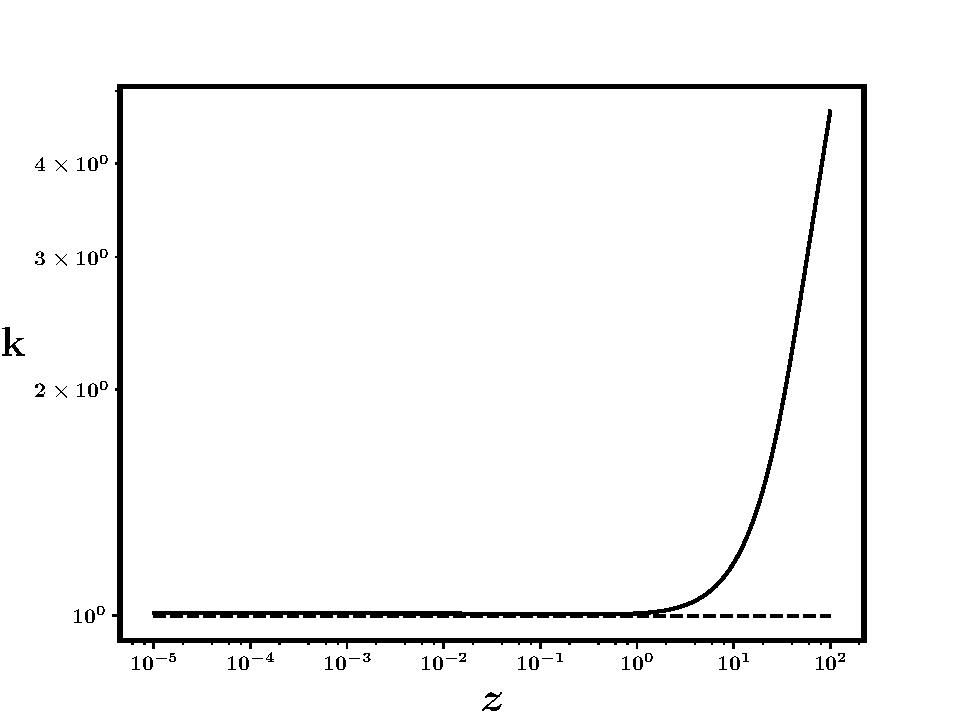
\includegraphics[scale=0.42]{k_correction--Fermi}
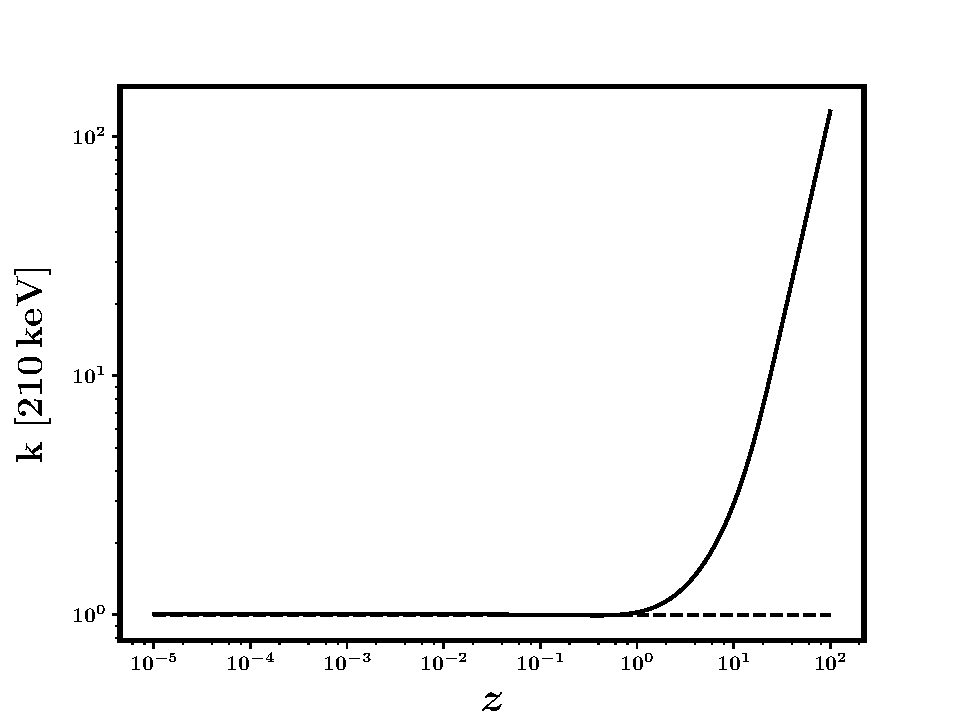
\includegraphics[scale=0.42]{k_correction--Swift}
\caption[$k$-correction factors for \f\ and \s]{The $k$-correction factors for \f\ [left] and \s\ [right], assuming average spectral parameters as derived from the sample of Fermi bursts: $<\Ep> \, = 181.3$ keV, $<\alpha> \, = -0.566$, $<\beta> \, = -2.823$. Since these average numbers are used, they do not include uncertainties. Note that the units of $k$ are different for the two missions owing to Equations \ref{eq:definition_of_k---Fermi--long} and \ref{eq:definition_of_k---Swift--long}. One also notices the striking difference in the scales: whereas it is much close to unity for \f, which is a wide-band detector, for \s, it is much larger for large redshifts than its value at the local universe, because of its limited energy-range.}
\label{fig:k-correction--long}
\end{center}
\end{figure}

To accurately derive the Yonetoku correlation, I first select the sub-sample of all \f\ and \s\ bursts that have accurate estimations of the Band function \citepalias{Band_et_al.-1993-ApJ} parameters during the prompt emission, by \f, as well as accurate redshift measurement by \s\ follow-up. Previous works have relied on modelling the spectral parameters by \s, which suffers from the limited wavelength range of BAT. I use the accurate spectral parameters from \f\ instead, reducing the inaccuracy of the estimates of luminosity. Moreover, due to the same reason, I also notice that the $k$-correction is very close to unity for these bursts, unless the redshift is not too large [even for $z = 10$, the factor is less than $1.5$]. This is illustrated in left of Figure \ref{fig:k-correction--long}. In comparison, the $k$-correction of \s\ is much larger for larger redshifts.



\subsection{Selecting the common GRBs}
\label{sec:selecting_common_GRBs}

\begin{figure}
\begin{center}
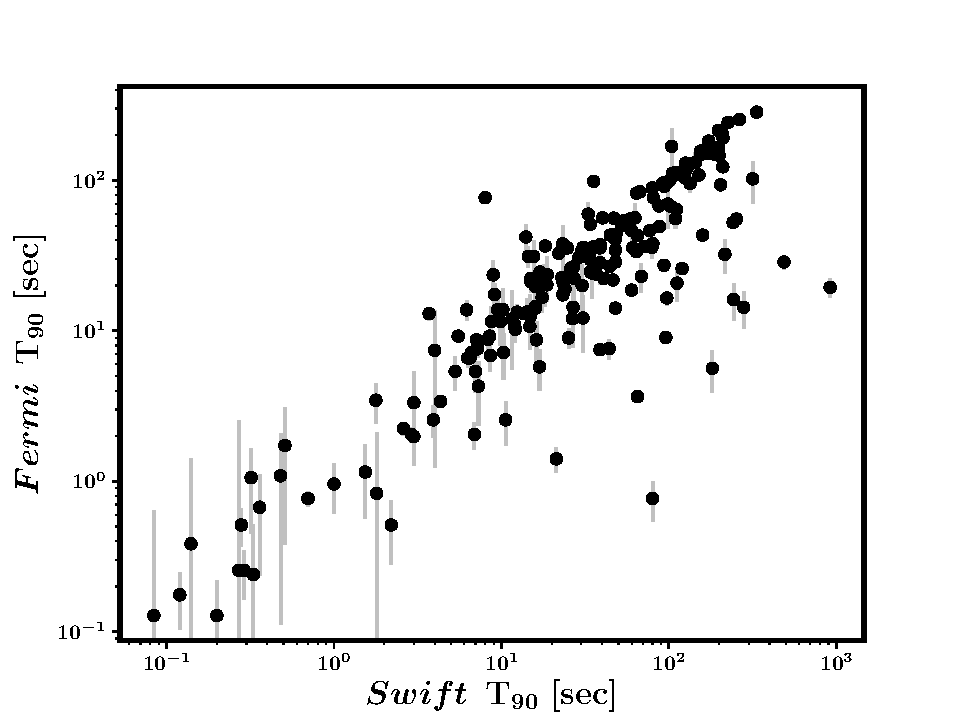
\includegraphics[scale=0.5]{comparing_T90s_of_common_GRBS--all}
\caption[Comparison of $\T$s of \f\ and \s\, GRBs]{Despite the expected correlation between the \f\ and \s\ $\T$s being observed, some GRBs have systematically smaller $\T$ in \f\ than \s. This has been investigated in detail, see Chapter \ref{chap:ongoing}.}
\label{fig:T90_comparison}
\end{center}
\end{figure}

The updated list of \f\ GRBs are selected from the \f\ catalogue\footnote{\url{https://heasarc.gsfc.nasa.gov/W3Browse/fermi/fermigbrst.html}} till GRB170501467, which includes $2070$ GRBs. Firstly, I choose only those bursts from the catalogue that have spectroscopically measured parameters for the GRB Band function, which includes $1729$ such cases. Then only those with small errors on the spectral parameters are chosen. For this, it is noted that the primary parameter that drive the error estimates in the luminosity is the $E_p$. Choosing only those with errors less than $100\%$ in $\Ep$, $1566$ bursts are retrieved.

The updated list of \s\ GRBs are selected from the \s\ catalogue\footnote{\url{https://swift.gsfc.nasa.gov/archive/grb_table/}} till GRB 170428A. The total number is $1021$, out of which those with firm redshift measurements is $312$.

Since the nomenclature of \f\ and \s\ GRBs are different, I select the following criteria for selecting the common GRBs. The difference between the trigger times are selected to be less than $10$ minutes, and they are restricted to within $10^{\circ} \times 10^{\circ}$ in RA and Dec for the two instruments. These numbers are empirically chosen, such that the common number of GRBs converge within a reasonable range of these cutoffs. This ensures I do not mistake two GRBs which are well separated in time and space to be the same GRB. Consequently I get $68$ common GRBs. Applying the $\T$ criterion for identifying short versus long bursts \citepalias{Kouveliotou_et_al.-1993-ApJ} separately for the two missions, I note that $65$ are long according to both \f\ and \s, two are short in both, while only one is short only in \f, GRB090927422 [\f\ nomenclature]. Its \f-$\T$ is $0.512 \pm 0.231$ s while that of \s\ is $2.2$ s. \f-$\T$s are calculated at higher energies and hence known to be systematically smaller in a handful of GRBs. Figure \ref{fig:T90_comparison} illustrates this effect. Hence, I choose this as a long burst. Moreover, this also gives me confidence to make the distinction between long and short GRBs based on the \s-criterion whenever it is available, i.e. for the other common GRBs [without redshift estimates from \s]. For the ones that are detected only by \f, I resort to applying the criterion based on the \f-$\T$.

It is to be noted that other spectroscopic models are also used for some GRBs, namely the powerlaw and the Comptonized model \citep{Gruber_et_al.-2014-ApJS--Fermi_catalogue}. Firstly, the Band function is itself a phenomenological combination of two powerlaws, and the single powerlaw fit is better for those GRBs in which the two powerlaw indices are very similar ($ \alpha \sim \beta$), which is automatically incorporated in the Band function phenomenology. The same is true for the Comptonized model, which is a subset of the Band function in the limit $ \beta \to - \infty$. Thus, not explicitly choosing the powerlaw and the Comptonized model fits instead of the Band function, in case they are available, does not alter the conclusions of this work.


\begin{longtable}{|c|c|c|c|c|}
%\begin{center}
\hline
GRB name & $\T$ & $z$ & $\Ep$ & $\Lp$ \\
 & [s] &  & [keV] & [$10^{52} \, \ergpersec$] \\
\hline
\hline
161129A & $  36.096 $ & $ 0.645 $ & $ 275.537 \pm 58.744 $ & $ 0.149 \pm 0.144$ \\
\hline
161117A & $ 122.178 $ & $ 1.549 $ & $  70.513 \pm  7.182 $ & $ 1.328 \pm 1.289 $ \\
\hline
161017A & $  32.256 $ & $ 2.012 $ & $ 416.6937 \pm 138.027 $ & $ 2.617 \pm 2.616 $ \\
\hline
161014A & $  36.609 $ & $ 2.823 $ & $ 202.0655 \pm  27.06123$ & $ 5.101 \pm 4.910 $ \\
\hline
160804A & $ 131.586 $ & $ 0.736 $ & $  86.650 \pm  58.736 $ & $  0.099 \pm  0.101 $ \\
\hline
151111A & $  46.336 $ & $ 3.500 $ & $ 108.430 \pm  44.195 $ & $  1.531 \pm  1.970 $ \\
\hline
150727A & $  49.409 $ & $ 0.313 $ & $  85.857 \pm  53.788 $ & $  0.010 \pm  0.010 $ \\
\hline
150403A & $  22.272 $ & $ 2.060 $ & $ 509.257 \pm  33.684 $ & $ 23.768 \pm 20.990 $ \\
\hline
150314A & $  10.688 $ & $ 1.758 $ & $ 298.023 \pm   9.405 $ & $ 31.814 \pm 27.856 $ \\
\hline
150301B & $  13.312 $ & $ 1.516 $ & $ 173.990 \pm  37.032 $ & $  0.814 \pm  0.801 $ \\
\hline
141225A & $   56.32 $ & $ 0.915 $ & $ 144.959 \pm  46.555 $ & $  0.187 \pm  0.185 $ \\
\hline
141221A & $  23.808 $ & $ 1.452 $ & $ 321.450 \pm 113.667 $ & $  1.106 \pm  1.117 $ \\
\hline
141220A & $   7.616 $ & $ 1.319 $ & $ 214.764 \pm  13.255 $ & $  2.209 \pm  1.994 $ \\
\hline
141004A & $    2.560 $ & $ 0.570 $ & $  31.427 \pm  10.465 $ & $  0.106 \pm  0.099 $ \\
\hline
140907A & $  35.841 $ & $ 1.210 $ & $ 100.911 \pm  20.217 $ & $  0.336 \pm  0.340 $ \\
\hline
140703A & $  83.969 $ & $ 3.140 $ & $ 231.937 \pm  68.781 $ & $  5.534 \pm  5.290 $ \\
\hline
140512A & $  147.97 $ & $ 0.725 $ & $ 574.600 \pm  95.107 $ & $  0.567 \pm  0.515 $ \\
\hline
140506A & $  64.128 $ & $ 0.889 $ & $ 137.908 \pm  21.044 $ & $  0.774 \pm  0.714 $ \\
\hline
140423A & $  95.233 $ & $ 3.260 $ & $ 176.398 \pm  85.904 $ & $  3.535 \pm  3.632 $ \\
\hline
140304A & $  31.232 $ & $ 5.283 $ & $ 165.164 \pm  91.630 $ & $  8.912 \pm  9.341 $ \\
\hline
140213A & $  18.624 $ & $ 1.207 $ & $  84.226 \pm   3.368 $ & $  2.686 \pm  2.391 $ \\
\hline
140206A & $  27.264 $ & $ 2.730 $ & $ 112.101 \pm   7.156 $ & $ 15.302 \pm 13.773 $ \\
\hline
131105A & $ 112.642 $ & $ 1.686 $ & $ 453.492 \pm  75.791 $ & $  3.201 \pm  2.939 $ \\
\hline
130612A & $   7.424 $ & $ 2.006 $ & $  22.641 \pm   7.169 $ & $  0.497 \pm  0.515 $ \\
\hline
130610A & $   21.760 $ & $ 2.092 $ & $ 150.169 \pm  55.755 $ & $  1.197 \pm  1.269 $ \\
\hline
130420A & $ 104.962 $ & $ 1.297 $ & $  58.717 \pm   6.266 $ & $  0.304 \pm  0.295 $ \\
\hline
121211A & $   5.632 $ & $ 1.023 $ & $ 111.291 \pm  44.987 $ & $  0.107 \pm  0.132 $ \\
\hline
121128A & $  17.344 $ & $ 2.200 $ & $ 115.306 \pm   6.532 $ & $  6.059 \pm  5.477 $ \\
\hline
120922A & $ 182.275 $ & $ 3.100 $ & $  65.404 \pm  24.027 $ & $  2.273 \pm  2.374 $ \\
\hline
120907A & $   5.760 $ & $ 0.970 $ & $ 133.896 \pm  42.997 $ & $  0.213 \pm  0.224 $ \\
\hline
120811C & $  14.336 $ & $ 2.671 $ & $  32.603 \pm   6.480 $ & $  2.663 \pm  2.633 $ \\
\hline
120119A & $  55.297 $ & $ 1.728 $ & $ 274.490 \pm  31.767 $ & $  5.603 \pm  5.007 $ \\
\hline
120118B & $  37.825 $ & $ 2.943 $ & $  67.133 \pm  12.698 $ & $  2.040 \pm  2.483 $ \\
\hline
111228A & $  99.842 $ & $ 0.714 $ & $  94.722 \pm  11.909 $ & $  0.393 \pm  0.363 $ \\
\hline
111107A & $  12.032 $ & $ 2.893 $ & $ 128.811 \pm  76.395 $ & $  1.874 \pm  2.251 $ \\
\hline
110818A & $  67.073 $ & $ 3.360 $ & $  54.891 \pm  34.483 $ & $  2.501 \pm  2.441 $ \\
\hline
110731A & $   7.485 $ & $ 2.830 $ & $ 176.569 \pm  15.040 $ & $ 18.900 \pm 17.240 $ \\
\hline
110213A & $  34.305 $ & $ 1.460 $ & $  81.154 \pm   9.576 $ & $  2.196 \pm  2.051 $ \\
\hline
110128A & $   12.160 $ & $ 2.339 $ & $ 323.481 \pm 206.884 $ & $  1.234 \pm  1.441 $ \\
\hline
101219B & $  51.009 $ & $ 0.551 $ & $  87.214 \pm  23.350 $ & $  0.027 \pm  0.030 $ \\
\hline
100906A & $ 110.594 $ & $ 1.727 $ & $ 146.327 \pm  25.180 $ & $  4.081 \pm  3.746 $ \\
\hline
100816A & $   2.045 $ & $ 0.803 $ & $ 131.919 \pm  23.638 $ & $  0.749 \pm  0.762 $ \\
\hline
100814A & $  150.53 $ & $ 1.440 $ & $ 128.188 \pm  28.528 $ & $  0.974 \pm  0.917 $ \\
\hline
100728B & $   10.240 $ & $ 2.800 $ & $  63.193 \pm  20.822 $ & $  3.575 \pm  3.430 $ \\
\hline
100728A & $ 165.378 $ & $ 1.567 $ & $ 445.710 \pm  56.038 $ & $  4.359 \pm  3.952 $ \\
\hline
100704A & $ 214.404 $ & $ 3.600 $ & $ 241.466 \pm  42.810 $ & $ 14.470 \pm 13.619 $ \\
\hline
100615A & $  37.377 $ & $ 1.398 $ & $  47.743 \pm   6.946 $ & $  0.857 \pm  0.800 $ \\
\hline
091208B & $   12.480 $ & $ 1.063 $ & $ 145.513 \pm  19.596 $ & $  1.578 \pm  1.425 $ \\
\hline
091127 & $   8.701 $ & $ 0.490 $ & $  55.452 \pm   2.278 $ & $  0.496 \pm  0.435 $ \\
\hline
091020 & $  24.256 $ & $ 1.710 $ & $ 239.827 \pm 142.685 $ & $  1.689 \pm  1.558 $ \\
\hline
090927 & $   0.512 $ & $ 1.370 $ & $  96.283 \pm  15.010 $ & $  0.663 \pm  0.810 $ \\
\hline
090926B & $  55.553 $ & $ 1.240 $ & $ 111.361 \pm  14.262 $ & $  0.344 \pm  0.380 $ \\
\hline
090618 & $ 112.386 $ & $ 0.540 $ & $ 425.860 \pm  23.611 $ & $  1.511 \pm  1.333 $ \\
\hline
090516A & $ 123.074 $ & $ 4.109 $ & $  69.685 \pm  50.160 $ & $  5.843 \pm  5.740 $ \\
\hline
090424 & $  14.144 $ & $ 0.544 $ & $ 186.906 \pm   5.695 $ & $  1.282 \pm  1.123 $ \\
\hline
090423 & $   7.168 $ & $ 8.000 $ & $  80.209 \pm  20.560 $ & $ 20.920 \pm 31.970 $ \\
\hline
090113 & $  17.408 $ & $ 1.749 $ & $ 202.131 \pm  44.730 $ & $  1.011 \pm  1.050 $ \\
\hline
090102 & $  26.624 $ & $ 1.547 $ & $ 378.267 \pm  22.980 $ & $  4.534 \pm  4.092 $ \\
\hline
081222 & $   18.88 $ & $ 2.700 $ & $ 167.492 \pm  19.223 $ & $ 10.369 \pm  9.500 $ \\
\hline
081221 & $  29.697 $ & $  2.260 $ & $ 115.650 \pm   4.717 $ & $ 10.079 \pm  9.069 $ \\
\hline
081121 & $  41.985 $ & $ 2.512 $ & $ 192.442 \pm  66.262 $ & $  5.149 \pm  4.758 $ \\
\hline
081008 & $ 150.015 $ & $ 1.968 $ & $ 173.257 \pm  48.589 $ & $  0.981 \pm  1.034 $ \\
\hline
080928 & $  14.336 $ & $ 1.692 $ & $  83.139 \pm  33.113 $ & $  0.525 \pm  0.613 $ \\
\hline
080916A & $  46.337 $ & $ 0.689 $ & $ 241.131 \pm  36.958 $ & $  0.172 \pm  0.168 $ \\
\hline
080810 & $ 107.457 $ & $ 3.350 $ & $ 734.928 \pm 488.746 $ & $  7.217 \pm  7.044 $ \\
\hline
080804 & $  24.704 $ & $ 2.204 $ & $ 162.808 \pm  32.111 $ & $  2.029 \pm  2.082 $ \\
\hline
\caption[Long GRBs used for re-deriving Yonetoku correlation]{The properties of the $66$ long GRBs used for re-deriving the Yonetoku correlation.}
\label{tab:LGRBs_for_Yonetoku_correlation}
%\end{center}
\end{longtable}




\subsection{Testing the correlation}

\begin{figure}
\begin{center}
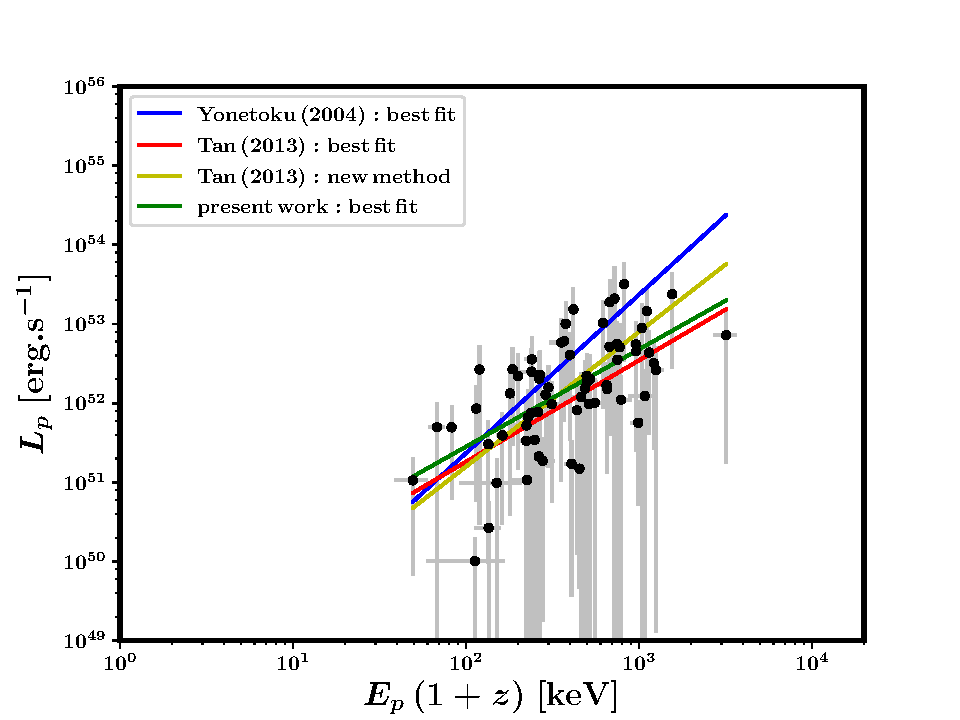
\includegraphics[scale=0.5]{L_vs_Ep0--correlations--my_bestfit}
\caption[Yonetoku correlation of long GRBs]{The Yonetoku correlation as seen from the data of $66$ long GRBs with accurate Band parameters from \f\ and redshift measurement from \s. The parameters of the correlation, from various studies, are over-plotted. I get the best-fit parameters of $A = 4.783 \pm 1.026$ and $\eta = 1.227 \pm 0.038$ for the the correlation defined in Equation \ref{eq:Yonetoku_correlation--long}.}
\label{fig:Yonetoku_correlation--long}
\end{center}
\end{figure}

\begin{figure}
\begin{center}
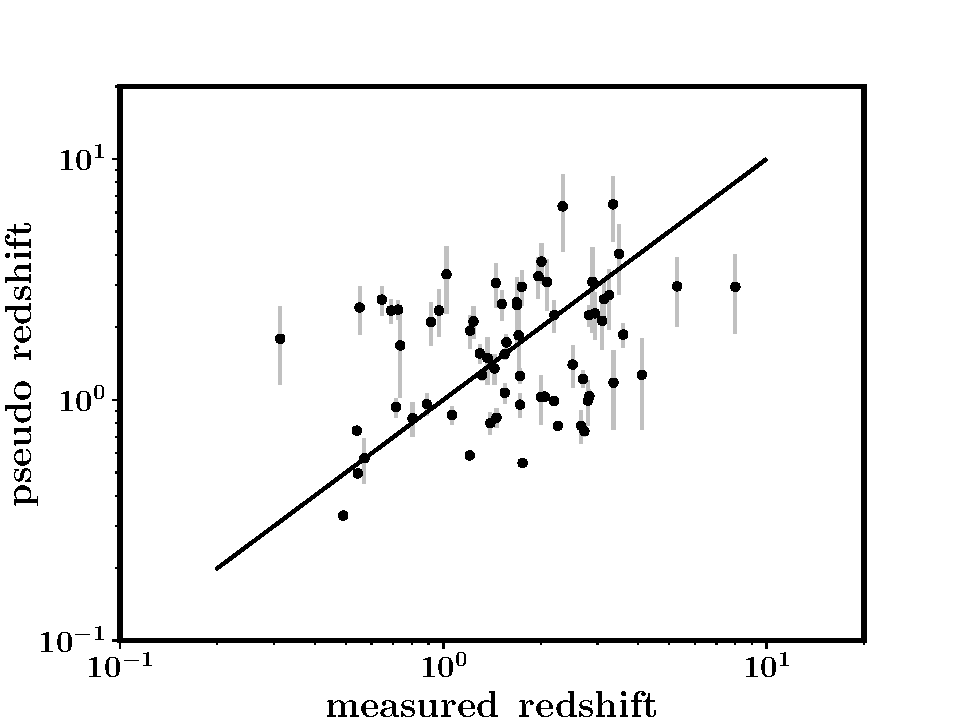
\includegraphics[scale=0.42]{redshift_comparison}
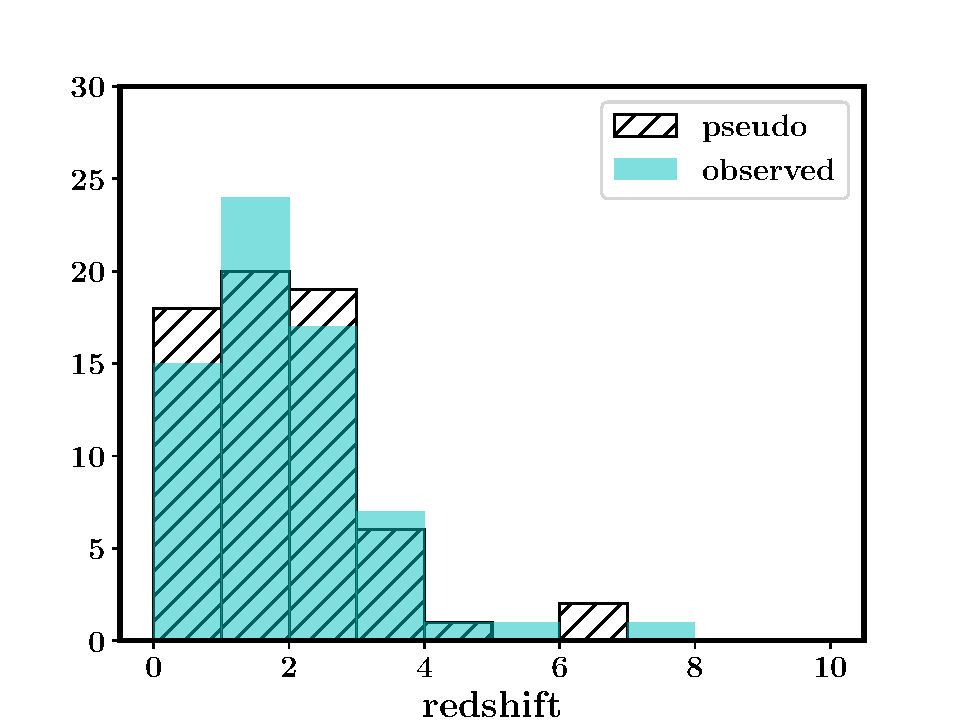
\includegraphics[scale=0.42]{distribution--my_bestfit}
\caption[Observed versus pseudo redshifts]{The redshift distribution for the $66$ long GRBs chosen in our sample. \eL: Individual comparison, the line indicating the expected relationship if the method was successful in predicting the pseudo redshifts accurately. \eR: Statistical comparison: filled [cyan] histogram shows the observed distribution, hatched [black] histogram shows the pseudo redshift distribution. The small discrepancies, specially at higher redshifts, can be easily understood to be due to the errors on the pseudo redshifts.}
\label{fig:redshift_distribution--bestfit}
\end{center}
\end{figure}

When I plot $\Lp$ versus $\Ep (1+z)$ [the factor of $(1+z)$ takes care of the transformation into the co-moving frame] for all the 68 GRBs, I notice that the only burst with systematically smaller $\Lp$ than the rest, is a short burst. Moreover, the sample of short GRBs with accurate spectral and redshift measures consists of only two cases. Hence, I do not attempt to study the correlation for short bursts separately. Moreover, I do not find any burst with luminosity lower than $10^{49} \, \ergpersec $, nor with $\T > 10^3$ s, and hence I do not attempt to segregate the possible separate classes of low-luminosity long GRBs [see for example \cite{Liang_et_al.-2007-ApJ}], or ultra-long GRBs [e.g. \cite{Levan_et_al.-2014-ApJ}].

I retrieve the Yonetoku correlation from the $66$ long bursts tabulated in Table \ref{tab:LGRBs_for_Yonetoku_correlation} to a high degree of confidence [a null-hypothesis of the Spearman correlation co-efficient of $0.623$ being false, ruled out with $p = 2.368 \times 10^{-8}$], as shown in Figure \ref{fig:Yonetoku_correlation--long}. The errors on $\Lp$ consist of errors in the flux as well as a conservative estimate of $70 \%$ systematic error added to all bursts, to take care of the inaccuracy in the spectral parameters. These parameters are non-linear and hence the errors cannot be calculated directly. The systematic error is chosen conservatively, since the changes in the spectral parameters always affect the estimates in $\Lp$ within a factor of $1.5$ even for the highest redshift bursts [see Figure \ref{fig:k-correction--long} for reference]. Also, if linear errors are propagated, the mean errors are again of the same order.

\begin{figure}
\begin{center}
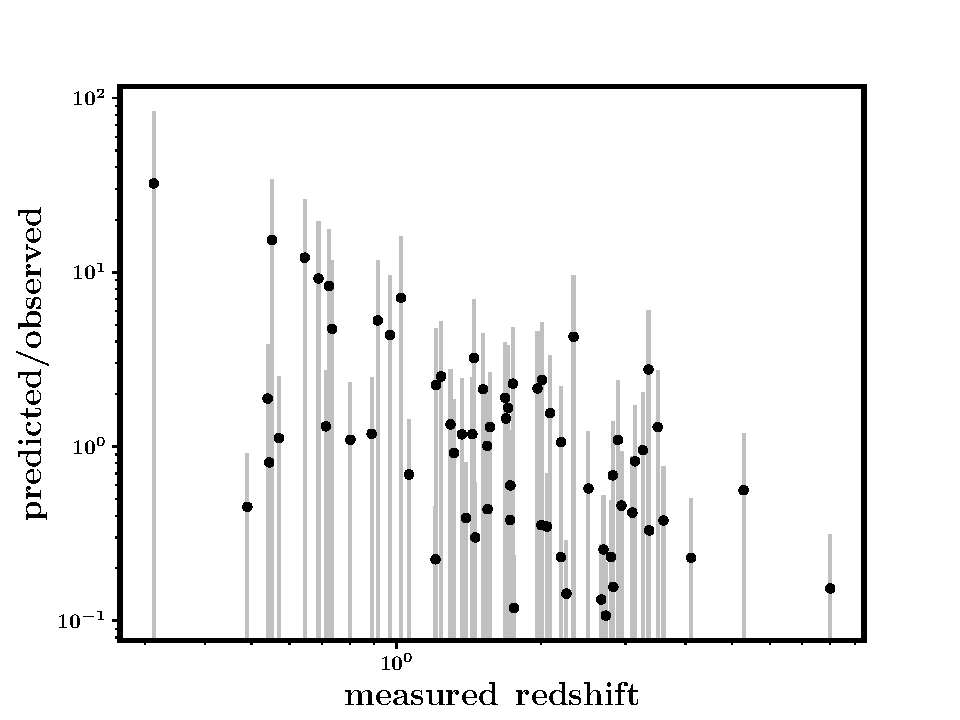
\includegraphics[scale=0.5]{scatter_with_measured_redshift--my_bestfit}
\caption[Systematic trend in the ratio of observed and predicted luminosities]{A strong anti-correlation is seen against the measured redshift, for the ratio between the luminosities predicted [from the best-fit Yonetoku correlation] and that measured directly.}
\label{fig:correlation_of_ratio_with_measured_z}
\end{center}
\end{figure}


For the Yonetoku correlation defined as 
\begin{equation}
\dfrac{ \Lp }{10^{52} \, \ergpersec} = A \left[ \dfrac{\Ep}{ {\rm MeV} } (1+z) \right]^{\eta},
\label{eq:Yonetoku_correlation--long}
\end{equation} I get the best-fit parameters of $A = 4.780 \pm 0.123$ and $\eta = 1.229 \pm 0.037$.

The pseudo redshift of any GRB can be obtained by numerically solving the simultaneous Equations \ref{eq:Luminosity_formula} and \ref{eq:Yonetoku_correlation--long}, given its flux $P$, and the spectral parameters $\alpha$, $\beta$, and $\Ep$.

The redshift distributions for the same $66$ GRBs in Table \ref{tab:LGRBs_for_Yonetoku_correlation}, both statistically and individually, are shown in Figure \ref{fig:redshift_distribution--bestfit}. It is noticed that although the method does not reproduce the redshifts on an individual basis, it is statistically reliable. The pseudo and observed redshifts have a median ratio of $1.002 \pm 0.721$, i.e. the number is consistent with unity. This is not an effect of normalization, as all the normalization factors are defined explicitly via Equation \ref{eq:Yonetoku_correlation--long}. The reason of it being statistically reliable is that, the method produces the pseudo redshifts of a larger sample by assuming gross parameters from a smaller sample which is however unbiased. The systematic discrepancies for individual bursts can be ascribed to the scatter around the Yonetoku correlation, as discussed below.

\citetalias{Tan_et_al.-2013-ApJL} uses the set of parameters that reduce the discrepancy between the distributions of the observed and pseudo redshifts. This method tries to reconcile the problem by changing the parameters, while circumventing the actual problem, that the Yonetoku correlation is intrinsic scattered. This is best illustrated by the left panel of Figure \ref{fig:redshift_distribution--bestfit}. Moreover to verify their method, I run it on the current dataset, and no global minimum of the discrepancy between the distributions is found. Hence, instead of modifying the parameters, I investigate the possible reasons for the scatter.

To investigate the presence of systematics in the discrepancy between the observed and the pseudo redshifts, I look for possible correlations of the ratio of the predicted luminosity from the Yonetoku correlation with the physical parameters $\Ep (1+z)$ and the measured redshift. No correlation is found with the former, which confirms that the scatter in the Yonetoku correlation is intrinsic. However, I find a strong anti-correlation between the ratio and the measured redshift, as shown in Figure \ref{fig:correlation_of_ratio_with_measured_z}, with a null hypothesis of the Spearman correlation co-efficient of $-0.533$ being false, ruled out with $p = 4.056 \times 10^{-6}$. The following qualitative hypothesis is proposed to explain this trend. The luminosities predicted by the best-fit parameters of the observed correlation are the better physical estimates of the luminosity, physically correlating with the spectral peak. The scatter in the observed correlation between the quantities $\Lp$ and $\Ep$ [in the source frame] is due to the inadequacy of the definition of the luminosity, which needs to be corrected for physical factors like the beaming of the burst and the burst environment. This explanation, however, is qualitative and requires an in-depth analysis via modelling the possible physical effects, not attempted in the current work.


\section{The estimated luminosities}
\label{sec:The_estimated_luminosities--long}

I next calculate the luminosities of all the \f\ detected bursts. This includes the $66$ GRBs already used in Section \ref{sec:Yonetoku_correlation--long}, and the rest with spectral estimates from \f\ but without redshift estimates from \s\ [irrespective of they are detected by \s]. For the latter cases, pseudo redshifts are predicted via the Yonetoku correlation, using \f\ flux and $k$-corrections. However the \s-$\T$ criterion is applied to those with \s-detections to distinguish between the short and long classes. For the GRBs with only \s\ detections along with measured redshifts, I directly calculate the luminosity from the flux and redshifts from the same catalogue, and the \s\ $k$-corrections derived from the Band function parameters fixed at the average values of the \f\ distribution, given by $<\Ep> \, =181.3$ keV, $<\alpha> \, = -0.566$, $<\beta> \, = -2.823$. It is to be noted that the $k$-correction is not sensitive to these parameters, as long as they are within a reasonable range [see for example \cite{Preece_et_al.-2000-ApJS} for the study of \B\ bursts]. For those bursts detected only by \s\ and further lacking redshift measurements, I estimate the pseudo redshifts via the \s\ $k$-corrections and the Yonetoku correlation. Since $\Ep$ features explicitly in the correlation, they are randomly sampled from the distribution of the \f\ bursts. The justification for such an approach is again that the \f\ being a wide-band detector, samples out all possible values of $\Ep$.


In Figure \ref{fig:pseudo_redshifts_and_luminosities--long} is shown the $L$-$z$ distribution of all these cases. The instrumental sensitivities are given by Equation \ref{eq:Luminosity_formula} with $P = 8.0 \times 10^{-8} \, \ergpercmsqpersec$ for \f\ and $P = 0.2 \, \phpercmsqpersec$ for \s\ [for a $100$ keV photon, this is equivalent to $3.2 \times 10^{-8} \, \ergpercmsqpersec$]. These numbers are chosen empirically from the respective catalogues, and describe the lower cutoff well. This places confidence on the used method and the estimated luminosities, and I proceed to use them for modelling the luminosity function [in Section \ref{sec:Modelling_the_GRB_LF--long}]. The slopes of the two correlations are $1.584 \pm 0.002$ for \f\ and $1.834 \pm 0.002$ for \s. A few bursts [eight] fall below the sensitivity line, which may be ascribed to the fact that the spectral parameters are sampled randomly from the \f\ distribution, whereas the flux is measured by \s; also, the $k$-correction increases sharply with $z$ for \s. These bursts are removed from the sample for subsequent analysis.


\begin{table}
\caption[Categories of long GRBs used for modelling LF]{The type of \f\ and \s\ long GRBs used for modelling, and how they are referred. The total number is $2067$.}
\label{tab:GRB_numbers--long}
\begin{center}
\begin{tabular}{|c|c|c|c|}
\hline 
type & redshift measured & number & modelled as\\
\hline 
\hline 
both \f\ and \s & yes & 66 & \multirow{2}{*}{\f}\\
\cline{1-3} 
only \f, or both & no & 1278 & \\
\hline 
only \s & no & 499 & \multirow{2}{*}{\s}\\
\cline{1-3} 
only \s & yes & 224 & \\
\hline 
\end{tabular}
\end{center}
\end{table}


On an average, the pseudo redshifts have $ \sim 20 \% $ errors and the luminosities calculated from them have $ \sim 40 \% $ errors, after propagating errors in all the estimation steps. Theoretically, the redshifts and hence luminosities of the \s\ bursts have much larger uncertainties, because their $\Ep$s are not known. However, this fact is ignored, to use these bursts in the statistical sense, laying no claim to the accuracy of the individual pseudo redshifts.

I also note that the distribution of pseudo redshifts and corresponding luminosities are relatively insensitive to the exact value of the parameters used for the Yonetoku correlation, as long as they are not significantly different from the best-fit estimates. The advantage of using this method lies in the fact that it evades the complex observational biases that plague and limit the study of redshift measured bursts. Also, it allows the model to take care of the instrumental thresholds while modelling the luminosity function via Equation \ref{eq:definition_of_phi}, to which I turn next.






\section{Modelling the long GRB luminosity function}
\label{sec:Modelling_the_GRB_LF--long}
For the purpose of modelling the luminosity function, the GRBs [$27$ in number] that have pseudo redshift greater than $10$ are not considered. The final number of GRBs used are showed in Table \ref{tab:GRB_numbers--long}. Also, the modelling is carried out separately for \f\ and \s, since the cut-off luminosities which feature in the model, via Equation \ref{eq:definition_of_phi}, are different for the two instruments, as discussed in Section \ref{sec:The_estimated_luminosities--long}. For each instrument, I bin the data into three equipopulous redshift bins: $0 < z <1.538$, $1.538 \leq z < 2.657$, $2.657 \leq z < 10.0$ for \f, and $0 < z < 1.809$, $1.809 \leq z <3.455$, $3.455 \leq z < 10.0$ for \s. It is to be noted that the errors on $N(L)$ are proportionally large, due to the large percentage errors on the derived luminosities, which are propagated across the bins.


\begin{figure}
\begin{center}
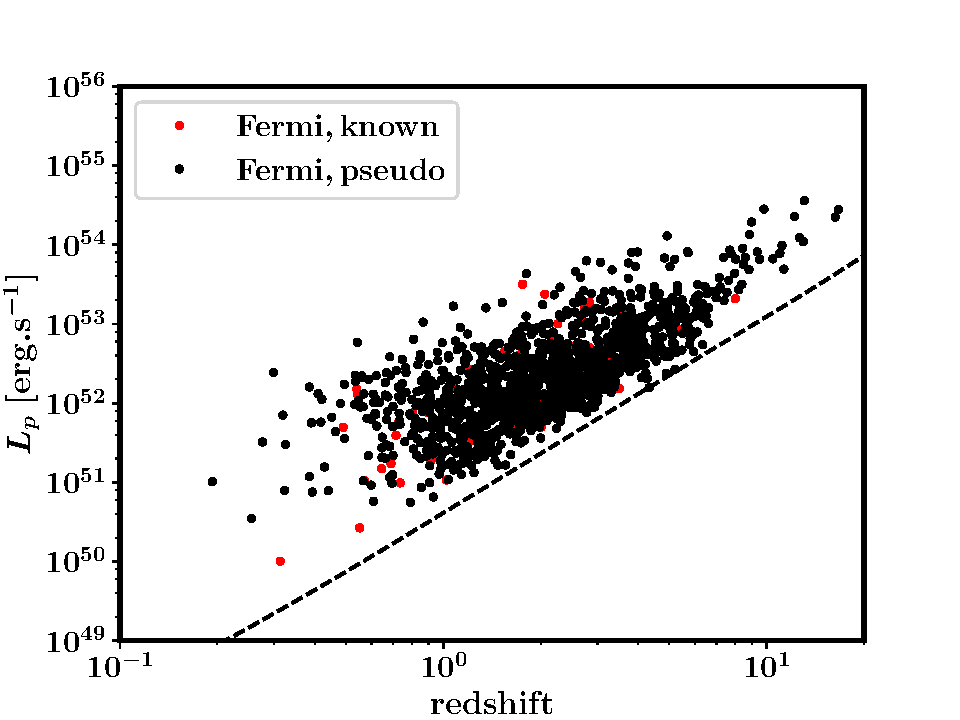
\includegraphics[scale=0.42]{L_vs_z--Fermi_long_all}
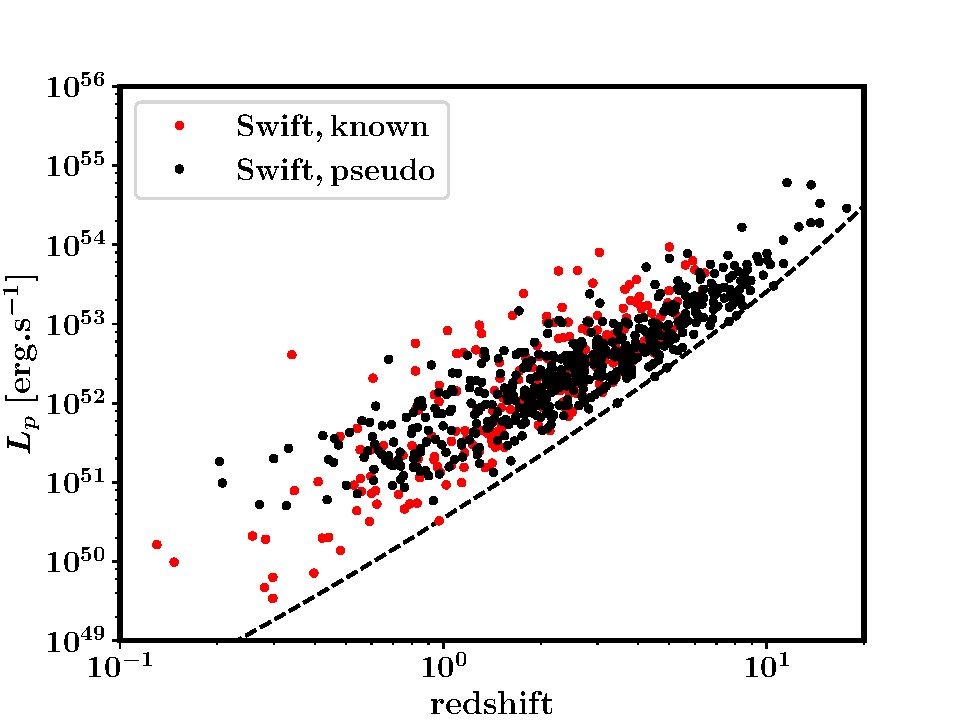
\includegraphics[scale=0.42]{L_vs_z--Swift_long_all}
\caption[Luminosity versus redshift of all long GRBs]{The luminosity versus redshifts of all GRBs. The red points are for those with redshift measurements, while black points are for those whose pseudo redshifts are derived as described in the text. The dotted lines show the corresponding instrumental sensitivity limits. The errors are not shown for the purpose of better visibility. \eL: For the GRBs that are detected by \f, irrespective of \s\ detection, including those with known redshifts [the 66 cases considered to study the correlation]. For all these bursts, the \f\ $k$-correction is used, whereas the \s-$\T$ criterion is applied for those available. \eR: For the bursts with detection only by \s, including those with measured redshifts. See Table \ref{tab:GRB_numbers--long} for more details on the nomenclature.}
\label{fig:pseudo_redshifts_and_luminosities--long}
\end{center}
\end{figure}


In the most recent work on GRB LF, \cite{Amaral-Rogers_et_al.-2017-MNRAS} [hereafter \citetalias{Amaral-Rogers_et_al.-2017-MNRAS}] discuss various kinds of models. In particular, they test models in which the GRB formation rate is tied to a single population of progenitors via the cosmic star formation rate, another similar but distinct model where low and high luminosity GRBs are separated into two distinct classes, and a third kind where no assumption of the GRB formation rates are made. They conclude that a clear distinction between the three kinds of models cannot be asserted however. In the present work, I do not attempt to classify low and high luminosity GRBs for the reason that there is no clear evidence from the study in Section \ref{sec:Yonetoku_correlation--long}. Moreover, I assume that the GRB formation rate is proportional to the star-formation rate, because after all it is massive stars formed in the galaxies that later end their lives in GRBs. There may be an additional dependence on the redshift: most generally represented via Equation \ref{eq:R_dot--long}. I take the cosmic star-formation rate $\csfr (z)$ from \cite{Bouwens_et_al.-2015-ApJ} [hereafter \citetalias{Bouwens_et_al.-2015-ApJ}; see references therein for the values at different redshifts], and model additional dependencies of the normalization, that is the GRB formation rate per unit cosmic star formation rate [or the GRB formation efficiency], as 

\begin{equation}
\fB C(z) \propto (1+z)^{\epsilon}.
\label{eq:fB.C_of_z--long}
\end{equation} It is noted that the detailed processes involved in the formation of GRBs do not affect this treatment, which is similar to that followed by \citetalias{Tan_et_al.-2013-ApJL}. Within this framework, I attempt to fit two models: the exponential cut-off powerlaw [ECPL] model, described by

\begin{equation}
\Phi_z(L) = \Phi_{0}
\left( \frac{L}{\Lb} \right)^{-\nu} \exp \left[ -\left( \frac{L}{\Lb} \right) \right],
\label{eq:The_ECPL_model--long}
\end{equation} and the broken powerlaw [BPL] model, given as

\begin{equation}
\Phi_z(L) = \Phi_{0} \begin{cases}
\left( \frac{L}{\Lb} \right)^{-\nu_1}, & L \leq \Lb\\
\left( \frac{L}{\Lb} \right)^{-\nu_2}, & L > \Lb.
\end{cases}
\label{eq:The_BPL_model--long}
\end{equation} Moreover, most generally the `break-luminosity' $\Lb$ is allowed to vary with redshift, as

\begin{equation}
\Lb = \Lbn (1+z)^{\delta},
\label{eq:evolution_of_break_luminosity--long}
\end{equation} with the quantity $\Lbn$ describing the normalization at zero redshift, and $\delta$ describing the evolution with redshift. The quantity $\Phi_0$ normalizes the probability density function $\Phi(L)$, and is an implicit function of the redshift $z$ via the dependence on $\Lb$. The models are then described by Equations \ref{eq:definition_of_phi}, \ref{eq:R_dot--long}, \ref{eq:fB.C_of_z--long}, \ref{eq:The_ECPL_model--long}, \ref{eq:The_BPL_model--long} and \ref{eq:evolution_of_break_luminosity--long}, along with $\csfr$ extracted numerically from \citetalias{Bouwens_et_al.-2015-ApJ}.

I look for the best-fit parameters of each model for \f\ and \s\ GRBs separately, because they have different $L_c (z)$ as shown in Figure \ref{fig:pseudo_redshifts_and_luminosities--long} [refer to Table \ref{tab:GRB_numbers--long} for the classes].

For the case of the ECPL, it is noticed that any non-zero values of $\delta$ or $\chi$ [or both] decreases the quality of fit, for both \f\ and \s. This allows me to decrease the parameter-space into a 2-dimensional space of $\nu$ and $\Lbn$ [which is equal to $\Lb$ for $\delta = 0$.] In the case of the BPL however, the data strongly requires the inclusion of a positive-definite $\delta$ and a  negative-definite $\chi$. It is to be noted that the ECPL has one parameter less than the BPL, but allows the break to vary naturally, explaining why the data requires the additional dependencies on the parameters $\delta$ and $\chi$ for the BPL model.

I search for the solutions by computing $d_{z}^{2} = \sum_{L} \left[ N_{{\rm model}} \left(L, z\right) - N_{{\rm observed}} \left( L, z \right) \right]^{2}$ for each redshift bin, then evaluating the discrepancy $d^{2} = \sum_{z}d_{z}^{2},$ and finally looking for the model parameters that reduces $d^{2}.$ I optimize the search by first choosing a large grid of parameters with sufficiently small bins, and then gradually converge on the best-fit parameters by decreasing the search-space and bin-size at each run.

In the case of the ECPL, both the \f\ and \s\ runs converge to similar values of parameters, and are consistent within the deduced errors. The fits are generally poorer for the latter case, and also because \s\ detects a larger number of GRBs at higher redshifts due to its higher sensitivity compared to \f. This, however, is not directly taken into account in the modelling, being a limitation of the present work. This is because the exact mathematical form of the detection probabilities at various fluxes is not known. Hence, I tabulate the parameters from only the \f\ fits, in Table \ref{tab:ECPL_model_parameters--long}. The data are generally over-fitted, with the $\red$ for the two instruments being $0.116$ for \f\ and $0.539$ for \s. This is because of the large number of bursts with similar luminosities, all with similarly large uncertainties.


\begin{table}
\caption[Best-fit parameters for the ECPL model]{The best-fit parameters for the ECPL model, as found by search in the $2$-dimensional space of $\nu$ and $\Lbn$, compared to the equivalent model of the recent work of \citetalias{Amaral-Rogers_et_al.-2017-MNRAS}, with which we see an overall agreement.}
\label{tab:ECPL_model_parameters--long}
\begin{center}
\begin{tabular}{|c|c|c|c|}
\hline 
parameter & present work & \citetalias{Amaral-Rogers_et_al.-2017-MNRAS}\\
\hline 
\hline 
$\nu$ & $0.60 \pm 0.1 $ & $0.71 \pm 0.07$\\
\hline 
$\Lbn$ & $5.40_{-1.5}^{+2.0}$ & $4.02_{-0.96}^{+1.52}$\\
\hline 
\end{tabular}
\end{center}
\end{table} 

\begin{figure}
\begin{center}
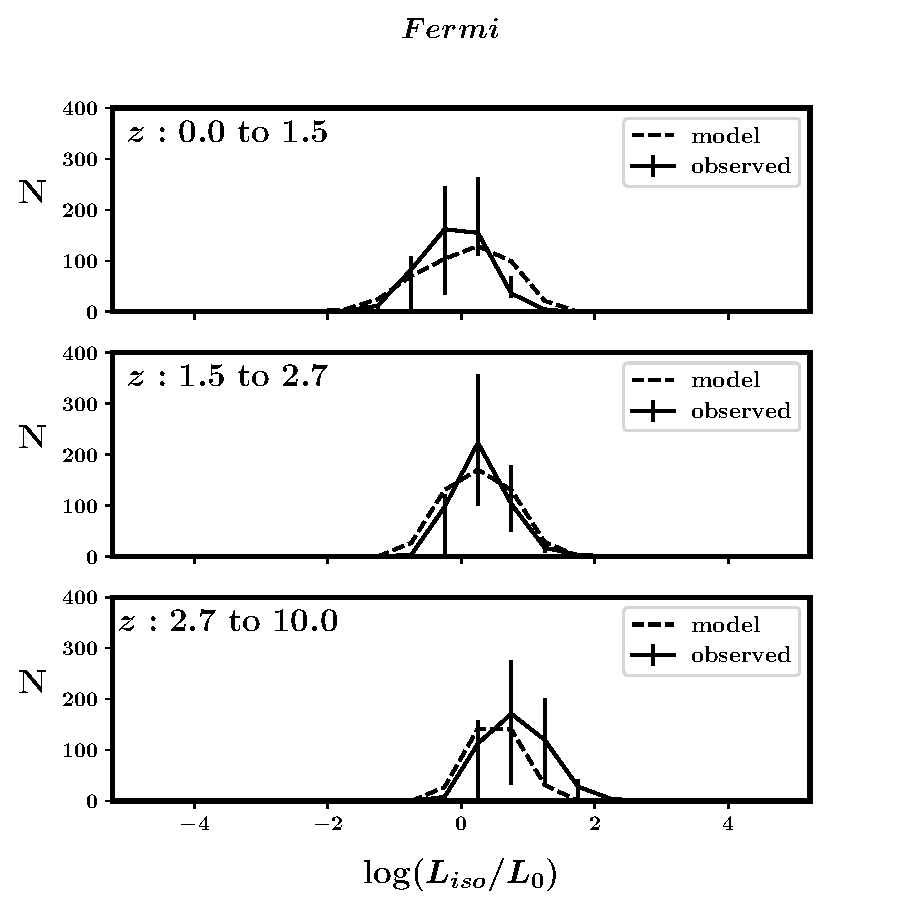
\includegraphics[scale=0.41]{ECPL--Fermi--binned}
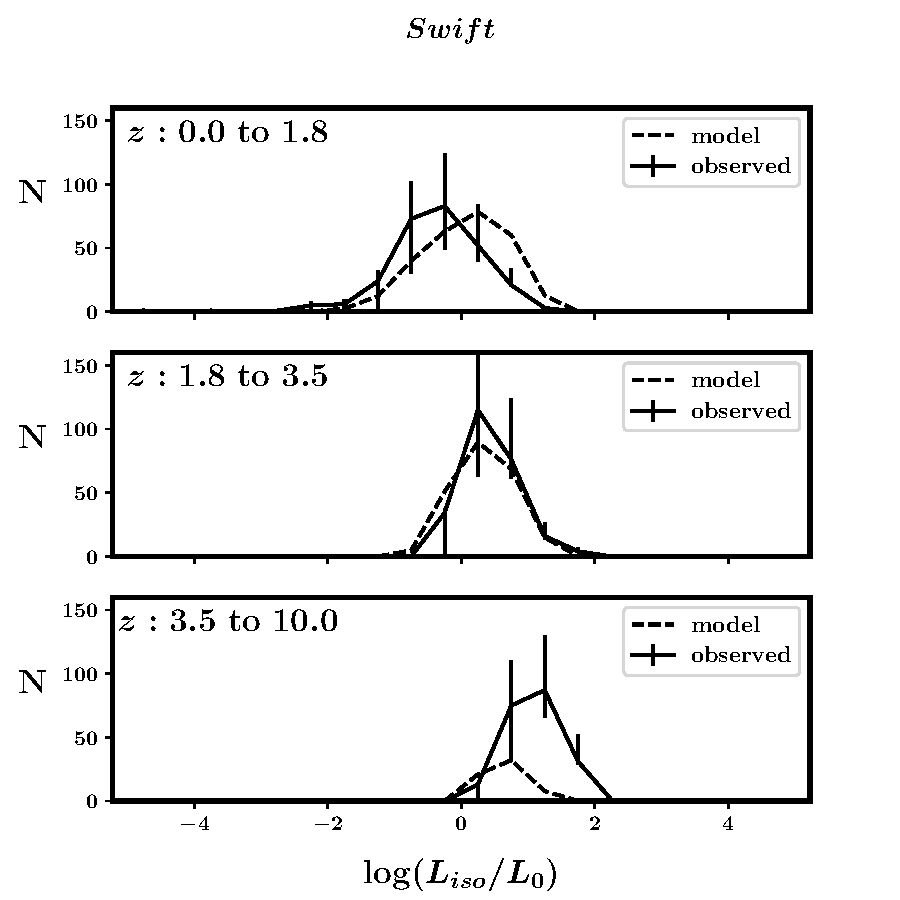
\includegraphics[scale=0.41]{ECPL--Swift--binned}
\end{center}
\begin{center}
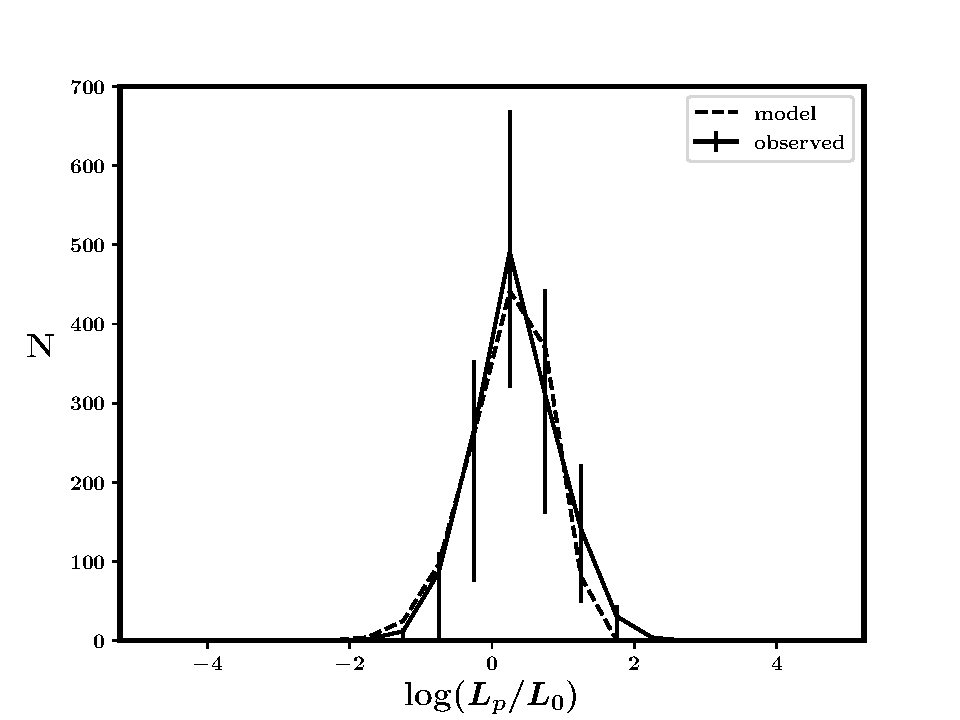
\includegraphics[scale=0.38]{ECPL--Fermi--total}
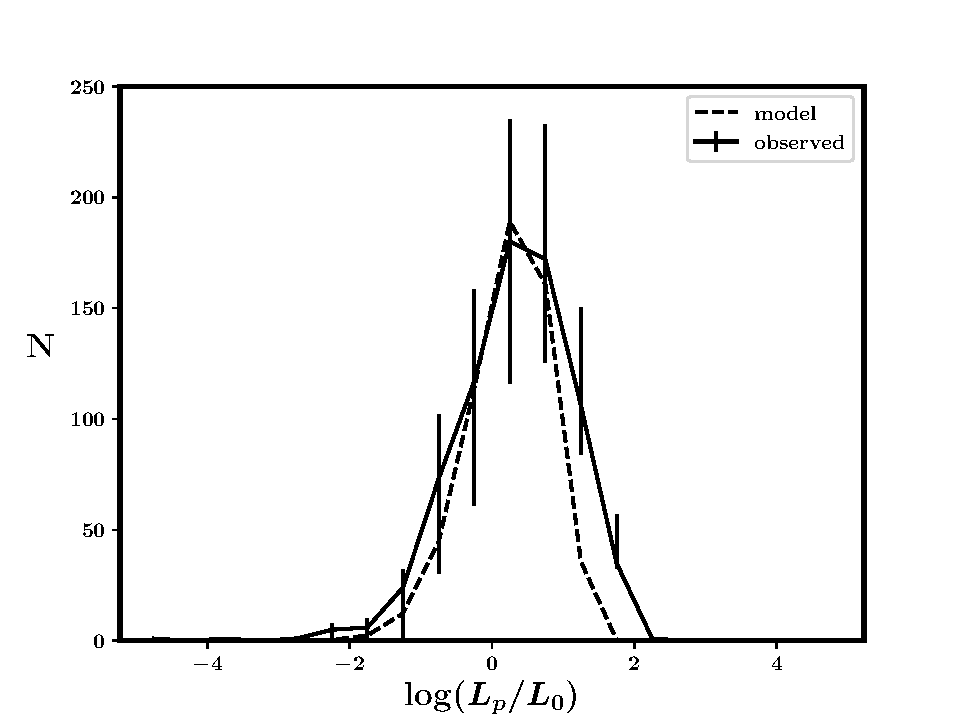
\includegraphics[scale=0.38]{ECPL--Swift--total}
\caption[Comparison of data and fits for the ECPL model]{The comparison of data and fits for the ECPL model, for \f\ [left] and \s\ [right]. Upper panels: Binned according to equipopulous redshift bins. Lower panels: Integrated over redshift, for the corresponding instruments in the upper panel. Here, $L_{0} = 10^{52} \, \ergpersec$. The `model' refers to that described in the text, with the final solutions of the parameters tabulated in Table \ref{tab:ECPL_model_parameters--long}. The errors are derived by taking into account the derived errors on luminosities.}
\label{fig:bestfit_ECPL_models--long}
\end{center}
\end{figure}

\begin{figure}
\begin{center}
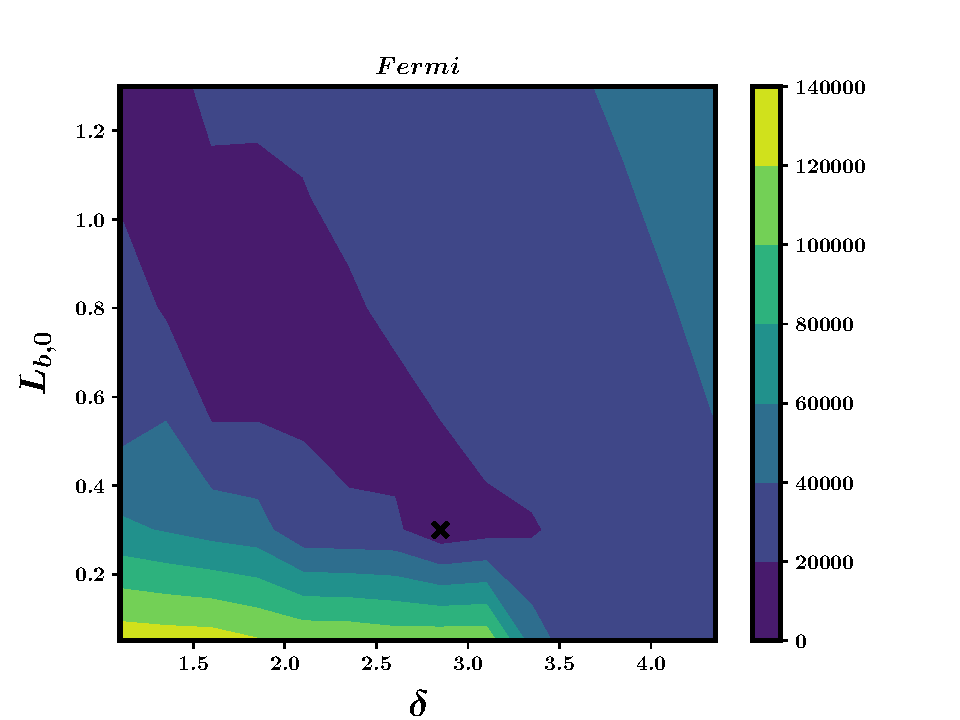
\includegraphics[scale=0.42]{discrepancy_contours--Fermi}
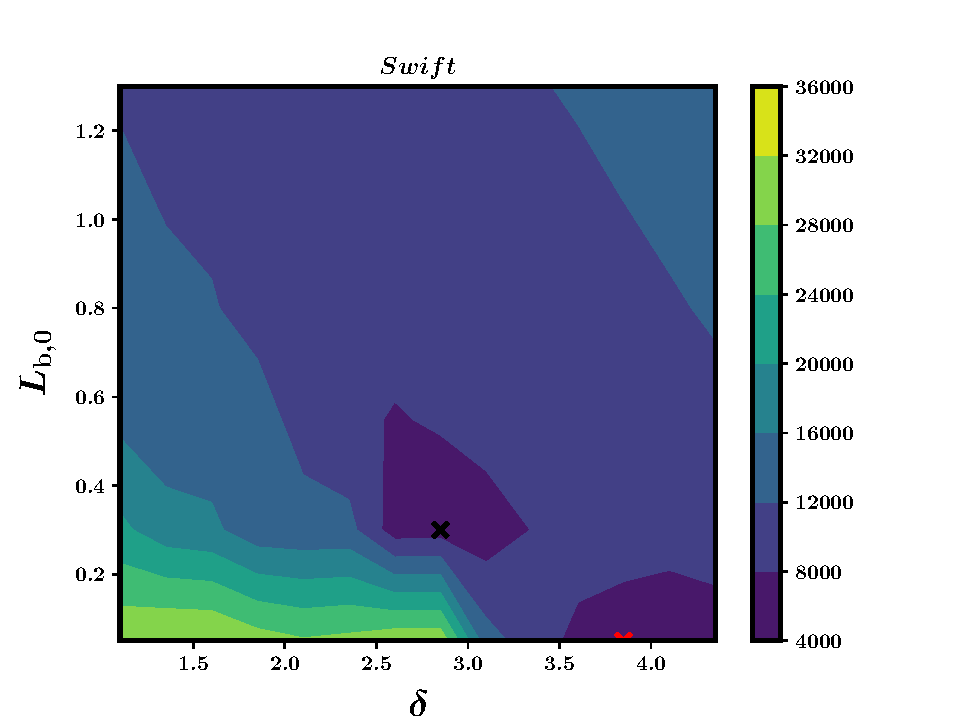
\includegraphics[scale=0.42]{discrepancy_contours--Swift}
\caption[$d^2$ contours for the BPL model]{The $d^2$  contours for the BPL model, for the two missions: \f\ [left] and \s\ [right], in the $\Lbn$-$\delta$ space. Marked in black-cross in both plots is the minimum discrepancy for \f, while in the \eR, the additional solution for \s\ has been marked in red-cross.}
\label{fig:discrepancy_contours}
\end{center}
\end{figure}



In the case of the BPL, there is no oscillation of any of the five parameters, justifying that the solutions are global. However it is found that \f\ and \s\ have different best-fits, significant differences being only in the related parameters $\nu_2$, $\Lbn$ and $\delta$. The \s\ solutions require extreme evolution of the break luminosity [$\delta = 3.95$], and raises suspicion of being an artefact of unaccounted systematics. Up on investigation it is found that the \s\ solutions are in fact degenerate with the \f\ solutions. The $d^2$ contours in the $\Lbn$-$\delta$ space have similar global shapes, and also behave similar locally around the \f\ solutions, see Figure \ref{fig:discrepancy_contours}. Thus I conclude that the best-fit solutions obtained for \s\ are driven by complications of its detection probability, and hence choose the \f\ best-fits as the accepted solutions, thus breaking the degeneracy. These are tabulated in Table \ref{tab:BPL_model_parameters--long}. The corresponding fits for the two instruments are shown in Figure \ref{fig:bestfit_BPL_models--long}. The larger proportional errors for \s\ make the $\red$ comparable for the two instruments however, $0.362$ for \f\ and $0.364$ for \s. This demonstrates that the use of \f\, bursts helps in solving the degeneracy of the parameter space of the model.



\begin{table}
\caption[Best-fit parameters for the BPL model]{The best-fit parameters for the BPL model, as found by extensive search in the $5$-dimensional space. The convergence of the parameters are tested thoroughly. As a comparison, I show the best-fit parameters for the equivalent model of the recent works of \citetalias{Amaral-Rogers_et_al.-2017-MNRAS} and \citetalias{Tan_et_al.-2013-ApJL}. Since the GRB formation rate is modelled differently in the former, the parameter $\epsilon$ cannot be compared. Moreover, one needs to be cautious to expect the other parameters to agree for the same reason. However, except $\nu_2$, reasonable agreement is found. The comparison is straightforward with \citetalias{Tan_et_al.-2013-ApJL}, which however does not cite errors on their parameters. An overall agreement is noticed between the two works.}
\label{tab:BPL_model_parameters--long}
\begin{center}
\begin{tabular}{|c|c|c|c|}
\hline
parameter & present work & \citetalias{Amaral-Rogers_et_al.-2017-MNRAS} & \citetalias{Tan_et_al.-2013-ApJL}\\
\hline 
\hline 
$\nu_1$ & $0.65_{-0.3}^{+0.1}$ & $0.69 \pm 0.09$ & $0.8$\\
\hline 
$\nu_2$ & $3.10_{-0.4}^{+0.5}$ & $1.88 \pm 0.25$ & $2.0$\\
\hline 
$\Lbn$ & $0.30_{-0.1}^{+0.15}$ & $0.15_{-0.09}^{+0.20}$ & $0.12$\\
\hline 
$\delta$ & $2.90_{-0.50}^{+0.25}$ & $2.04 \pm 0.45$ & $2$\\
\hline 
$\epsilon$ & $-0.80_{-1.0}^{+0.75}$ & - & $-1.0$\\
\hline 
\end{tabular}
\end{center}
\end{table}

\begin{figure}
\begin{center}
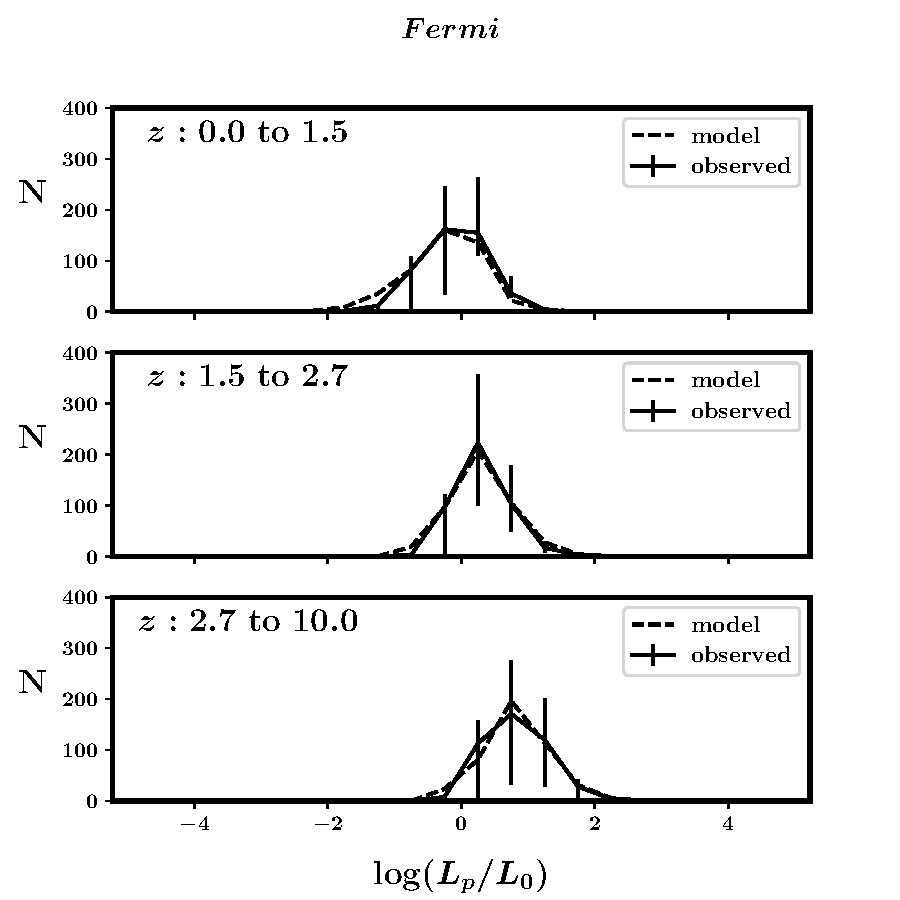
\includegraphics[scale=0.41]{BPL--Fermi--binned}
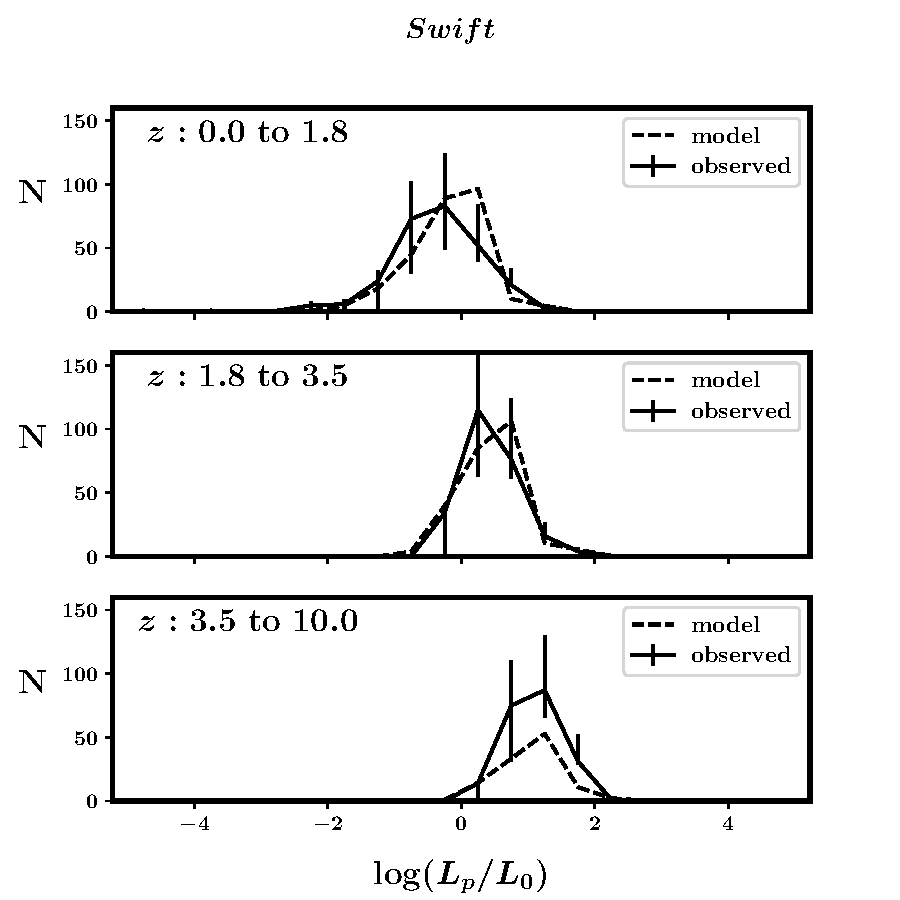
\includegraphics[scale=0.41]{BPL--Swift--binned}
\end{center}
\begin{center}
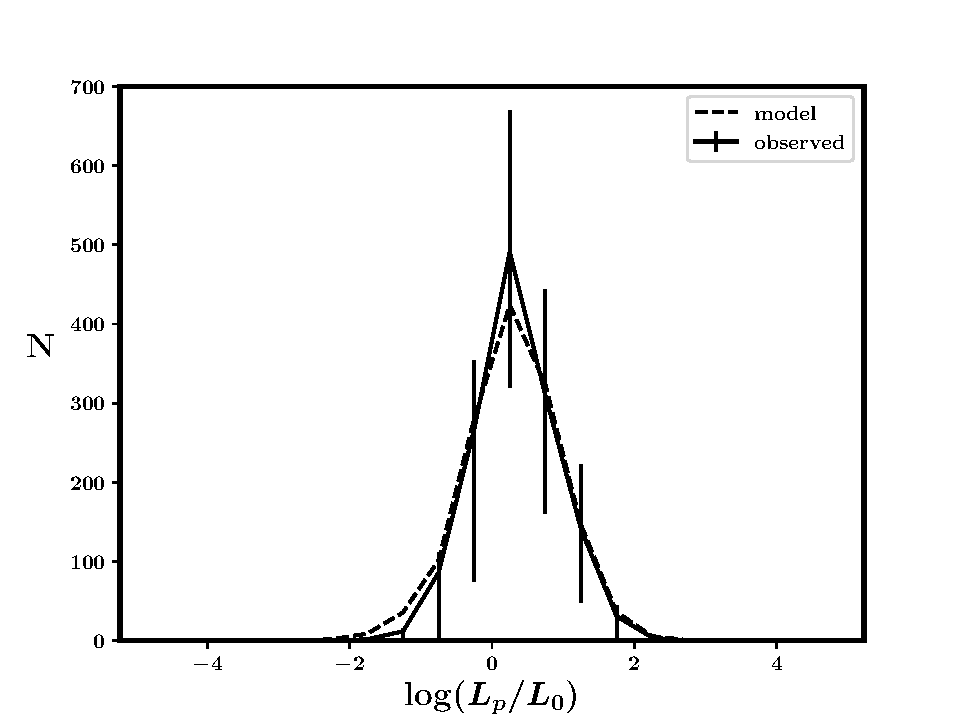
\includegraphics[scale=0.38]{BPL--Fermi--total}
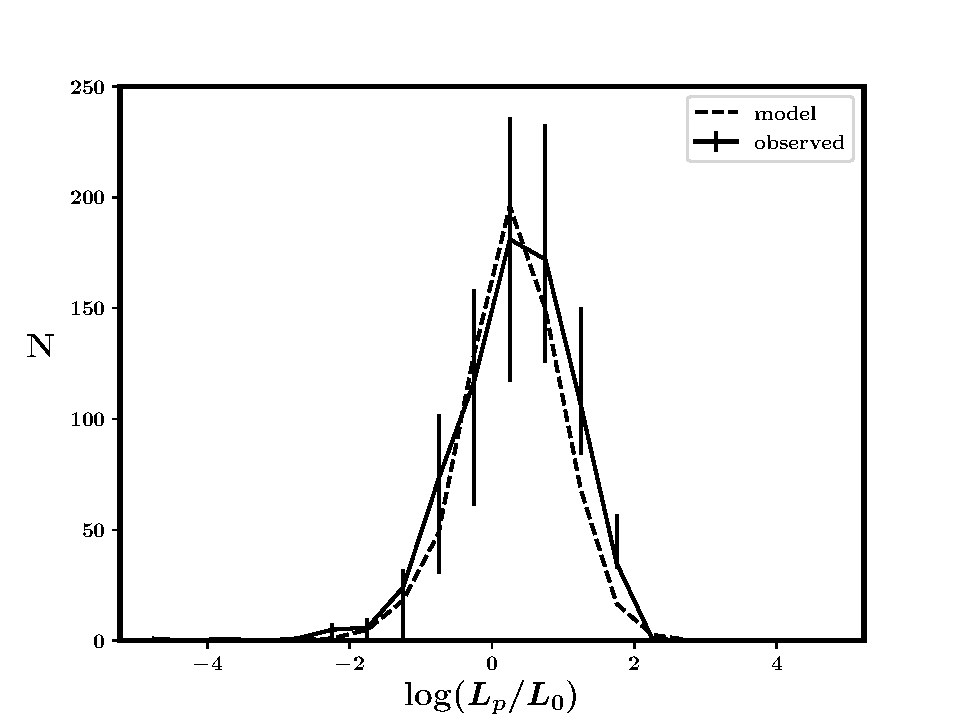
\includegraphics[scale=0.38]{BPL--Swift--total}
\caption[Comparison of data and fits for the BPL model]{Same as Figure \ref{fig:bestfit_ECPL_models--long}, for the BPL model. The parameters used for plotting are given in Table \ref{tab:BPL_model_parameters--long}.}
\label{fig:bestfit_BPL_models--long}
\end{center}
\end{figure}


Since the constant in the RHS of Equation \ref{eq:fB.C_of_z--long} is not known a priori, it is calculated via the solutions of the models. It is known that for \f, $T \sim 8.5$ yr and for \s, $T \sim 12$ yr. I assume $\frac{\Delta \Omega}{4 \pi} \sim \frac{1}{3}$ for \f\ and $\frac{1}{10}$ for \s, to get ratios of the observed and modelled numbers, which are converted to get

\begin{equation}
\fB C(0) = \begin{cases}
0.981 \times 10^{-8} \, \Msun^{-1}, & \f,\\
1.022 \times 10^{-8} \, \Msun^{-1}, & \s.
\end{cases}
\label{eq:fB.C_of_zero_ECPL--long}
\end{equation} for the ECPL model, and

\begin{equation}
\fB C(0) = \begin{cases}
0.597 \times 10^{-8} \, \Msun^{-1}, & \f,\\
0.653 \times 10^{-8} \, \Msun^{-1}, & \s.
\end{cases}
\label{eq:fB.C_of_zero_BPL--long}
\end{equation} for the BPL model. In \cite{Paul-2018-MNRAS--long} [hereafter \citetalias{Paul-2018-MNRAS--long}], the numbers are $4 \pi$ greater than this because of a human error in calculating the normalization. Combining all the ranges, one gets
\begin{equation}
\fB C(0) = [0.597, 1.022] \times 10^{-8} \, \Msun^{-1},
\label{eq:fB.C_of_zero--long}
\end{equation} which is slightly lower than $2.4 \times 10^{-8} \, \Msun^{-1}$ as quoted in \citetalias{Tan_et_al.-2013-ApJL}. However it is to be noted that since they have not provided any uncertainties on their numbers, any reasonable comparison is impossible. When multiplied with $\csfr(0)$, one can constrain the LGRB formation rate in the local universe to
\begin{equation}
\Rdot(0) = [0.12, 0.20] \, \pyG.
\label{eq:Rdot0--long}
\end{equation} \citetalias{Amaral-Rogers_et_al.-2017-MNRAS} has constrained $\Rdot(0)$ to $[0.04, 0.24] \, \pyG$. My constraints are thus more tighter.

The ECPL shows agreement with the most recent work of \citetalias{Amaral-Rogers_et_al.-2017-MNRAS}. The BPL model shows a sharp change at its break, which itself evolves quite strongly with redshift as $\Lb \sim 0.3 \times 10^{52} \, \ergpersec (1+z)^{2.90}$, in general agreement with \citetalias{Amaral-Rogers_et_al.-2017-MNRAS}. The GRB formation rate for a given star-formation rate decreases with increasing redshift as $\fB C \propto (1+z)^{-0.80}$ [the normalization is given by Equation \ref{eq:fB.C_of_zero--long}], in agreement to the reports of \citetalias{Tan_et_al.-2013-ApJL}. Whereas the ECPL automatically takes into account the variation of the break, this needs to be incorporated via  strong evolutions with redshift in the BPL model. However, it is not possible to distinguish between the two models based on the fits. One of the reasons is that the data are generally over-fitted due to the large uncertainties, and another possible reason being that the discrepancies between data and model could be a result of the complex nature of detection probabilities of the instruments, which I have not attempted to model directly.

It is to be noted that the present work is empirical; it does not attempt to provide an understanding of the models used, nor of the derived values of the parameters. A thorough understanding of the observed GRB number distribution requires one to justify the models via the phenomenology of long GRBs, taking into consideration the beaming of GRB jets and the GRB formation environment. This is the scope of future work.



\section{Predictions for \AS, \A, and \D}
\label{sec:predictions--long}

\subsection{\AS-CZTI}
\label{subsec:predictions_for_CZTI--long}
The CZT Imager or CZTI \citep{Bhalerao_et_al.-2017-JApA}, on the Indian multi-wavelength observatory \AS\ \citep{Rao_et_al.-2016-arXiv-Astrosat} is capable of detecting transients at wide off-axis angles, localizing them to a few degrees, and carrying out spectroscopic and polarization studies of GRBs, as demonstrated in \cite{Rao_et_al.-2016-ApJ}. A preliminary analysis done with the weakest GRB detected by CZTI suggests that it is at least as sensitive as \f, which detects roughly $3$ times the number of GRBs per year compared to \s. Similar to \f, the CZTI is also a wide-field detector. Moreover, it covers a wide energy range, being the most sensitive between $50$ and $200$ keV. Thus, it is reasonable to assume that its GRB detection rate is at least comparable to that of \s. Assuming this, I make predictions for CZTI over the redshift bins that were chosen for \f. The best-fit ECPL model predicts that CZTI should detect $150$ GRBs per year. The best-fit BPL model predicts detection-rate of around $140$ GRBs per year, with the \f\ equipopulous redshift bins almost equipopulous for CZTI as well. In $\sim 1.3$ years of operation, $\sim 100$ GRBs has been detected by CZTI by triggered searches alone\footnote{See a comprehensive list at \url{http://astrosat.iucaa.in/czti/?q=grb}.}, however the exact number is subjective. An automated algorithm to detect GRBs is being thoroughly tested and implemented, the details of which will be reported elsewhere. In the view of this, the predictions point out the fact $\sim 20$-$30$ GRBs are yet undiscovered from the CZTI data.

\subsection{Soft X-ray instruments}
\label{subsec:predictions_for_soft_Xray_instruments--long}
In this section I will describe work done after the publication of \citetalias{Paul-2018-MNRAS--long}, inspired by looking at the GRB-detection capabilities of the future ESA mission \A\footnote{\url{https://www.the-athena-x-ray-observatory.eu/}}, and also an Indian GRB-dedicated mission currently in the planning stage [PI: Professor Varun Bhalerao, IIT-Bombay], called the \D. \A\ will have a soft X-ray detector on-board, called the `Wide Field Imager' [WFI] that will have excellent timing capabilities, and improved detection sensitivity compared to previous soft X-ray missions like \X\, and \C. In view of this, it becomes important to answer the following question? How many LGRBs will \A -WFI detect per year? One would like to see if the number is significantly larger than that possible by \X\, and \C. Hence, the predictions of the detection rate of ``typical'' LGRBs, i.e. those with $10$ s durations were made assuming the characteristics of the instruments as detailed below.

\begin{itemize}
\item \X: EPIC-PN is the go-to instrument because the others [EPIC-MOS and RGS] do not have timing capabilities\footnote{\url{https://xmm-tools.cosmos.esa.int/external/xmm_user_support/documentation/uhb/epicmode.html}}. For this instrument, different sensitivities are quoted for the different energy ranges\footnote{\url{https://xmm-tools.cosmos.esa.int/external/xmm_user_support/documentation/uhb/epicsens.html}}, but for the purpose of GRBs, one can limit themselves to the ``hard'' to ``very hard'' range of $2$-$10$ keV with a sensitivity of $\sim 10^{-14} \, \ergpercmsqpersec$ for a $1$ Ms [$= 10^{6}$ s] observation, translating to a $10$ s sensitivity of $\sim 10^{-9} \, \ergpercmsqpersec$ [$s \propto t$\footnote{\url{https://xmm-tools.cosmos.esa.int/external/xmm_user_support/documentation/uhb/epicsens.html}}]. The field-of-view [FOV] is $33' \times 33'$\footnote{\url{https://heasarc.gsfc.nasa.gov/docs/xmm/xmm.html}}.

\item \C: For ACIS, the temporal resolution is poor or else there is severe compromise on positional information\footnote{\url{http://cxc.harvard.edu/cal/Acis/index.html}}. [The sensitivity is $\sim 10^{-13} \, \ergpercmsqpersec$ for $10^{3}$s, which translates to $\sim 10^{-11} \, \ergpercmsqpersec$ for $10$ s.] Hence I only consider HRC, for which time resolution is reasonable\footnote{\url{http://cxc.harvard.edu/cal/Hrc/index.html}}. For HRC-I, the bandwidth is $0.08$-$10$ keV, and FOV is $30' \times 30'$. For $10^{3}$ s, the sensitivity is $\sim 10^{-13} \, \ergpercmsqpersec$ (\C\, Proposers Observatory Guide, Page 130, Figure 7.11), which for $10$ s becomes $\sim 10^{-11} \, \ergpercmsqpersec$, two orders better than \X /EPIC-pn. Although HRC-S has much better temporal-resolution [and similar bandwidth but FOV of $6' \times 30'$], its ACS is not functional, hence only HRC-I was considered.

\item \A: The \A -WFI will have an energy range of $0.3$-$15$ keV, and a FOV of $40' \times 40'$, largest amongst the three. The scaled $10$ s sensitivity is $2 \times 10^{-12}$, better than even \C -HRC-I.
\end{itemize}

The sensitivity for all the instruments are shown in Figure \ref{fig:sensitivity_plots_for_soft_and_hard_instruments}, \eL. The combined predictions of the BPL and ECPL models, including uncertainties, are given in Table \ref{tab:predictions_for_soft_X-ray_instruments}.


\begin{table}
\caption[Long GRB detection rates by soft X-ray instruments]{Estimations and predictions of typical LGRB detection rates by the past, present and future soft X-ray instruments, combining the BPL and ECPL models and including uncertainties for both the models.}
\label{tab:predictions_for_soft_X-ray_instruments}
\begin{center}
\begin{tabular}{|c|c|}
\hline 
Instrument & Predicted numbers\\
 & [$\py$]\\
\hline
\hline
\X /EPIC-pn & $11$-$13$\\
\hline
\C /HRC-I & $10$-$14$\\
\hline
\A /WFI & $16$-$20$\\
\hline
\end{tabular}
\end{center}
\end{table}

\begin{figure}
\begin{center}
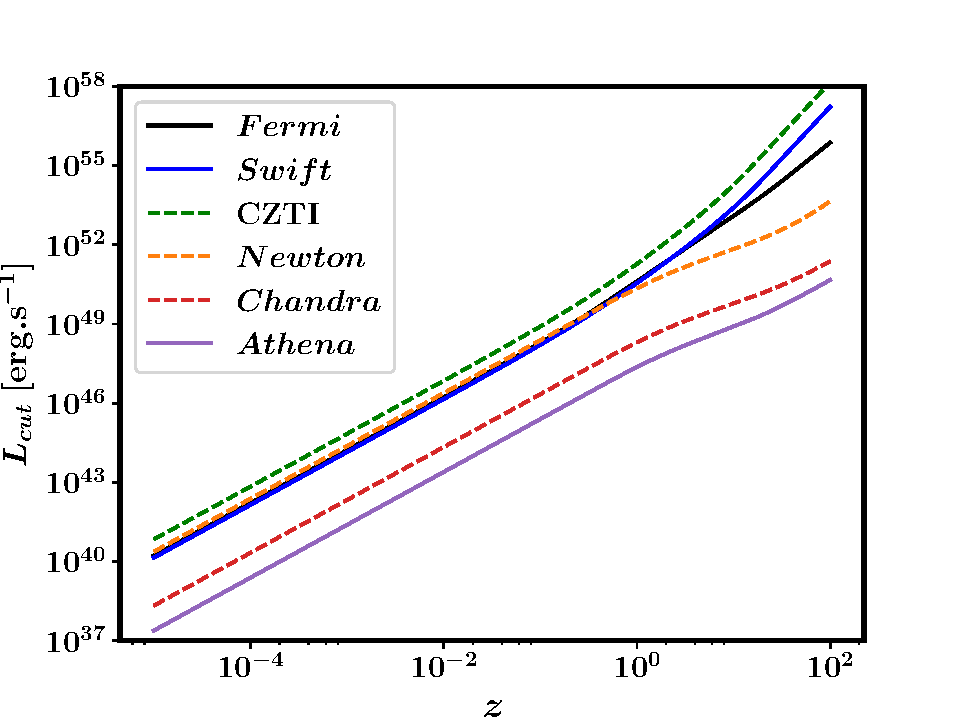
\includegraphics[scale=0.42]{sensitivity_plot--with_Swift_and_CZTI}
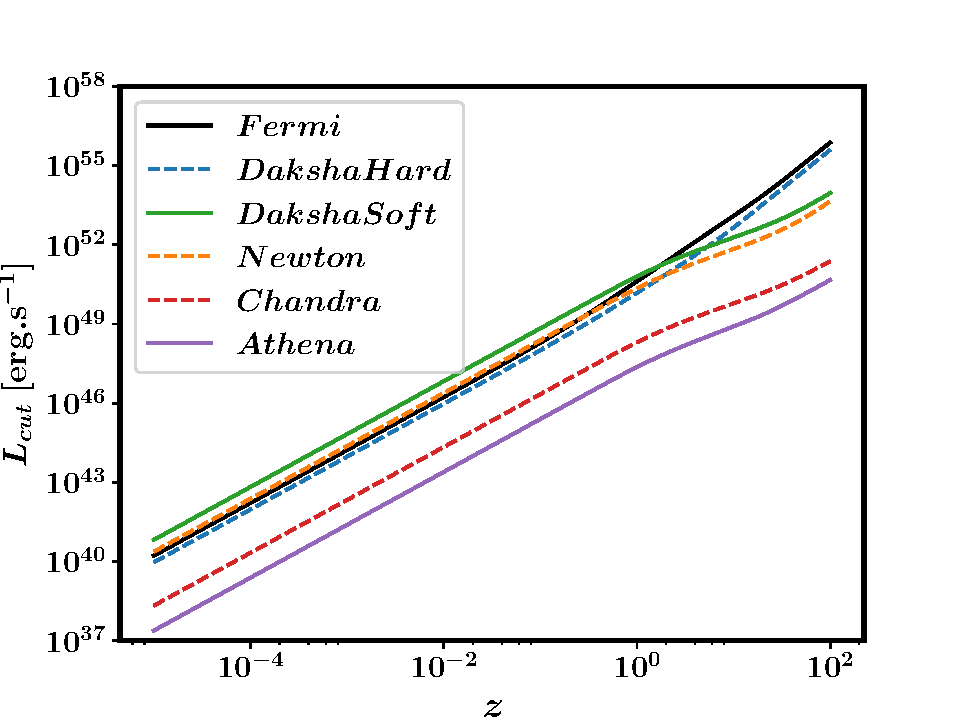
\includegraphics[scale=0.42]{sensitivity_plot--soft_Xray_instruments}
\caption[Sensitivity of several detectors to long GRBs]{\eL: The sensitivity for a ``typical'' long GRB [$10$ s] of the soft X-ray instruments compared to existing hard X-ray instruments; \eR: compared to both the proposed soft and hard X-ray instruments on \D.}
\label{fig:sensitivity_plots_for_soft_and_hard_instruments}
\end{center}
\end{figure}

\begin{figure}
\begin{center}
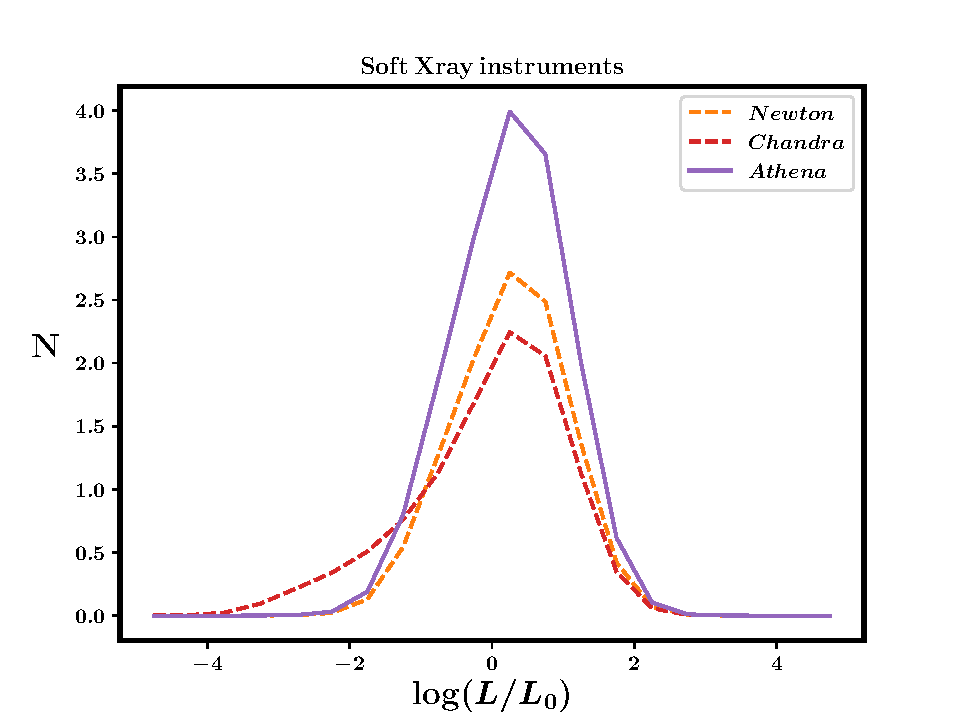
\includegraphics[scale=0.42]{predictions--long--BPL}
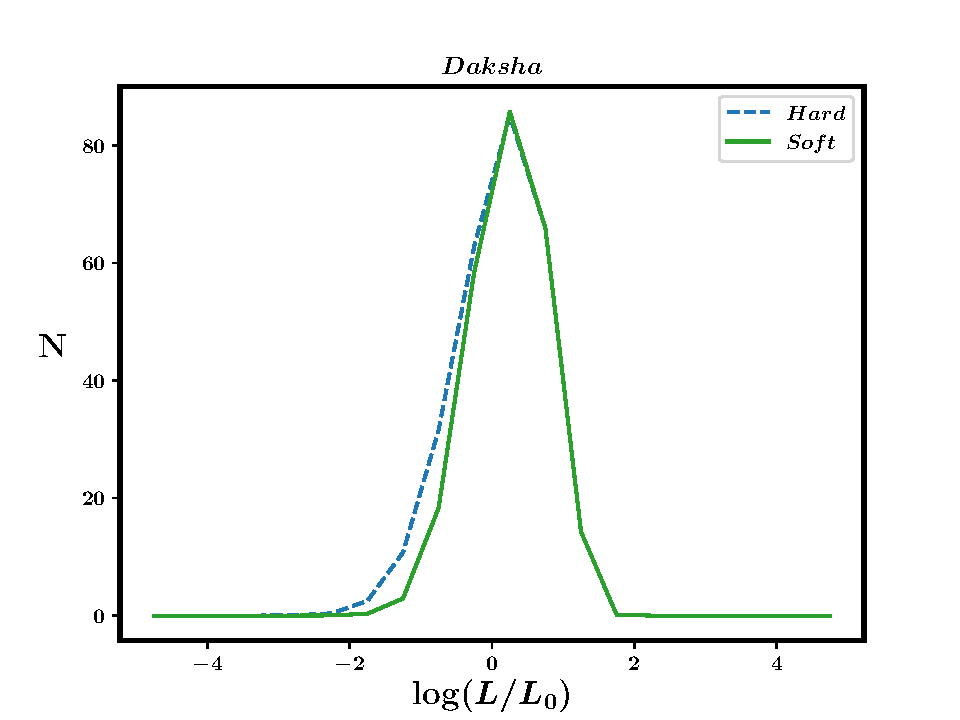
\includegraphics[scale=0.42]{predictions--long--ECPL}
\caption[Predictions for the luminosity distributions for several GRB detectors]{Predictions for the luminosity distribution of the long GRBs observed by different soft-X-ray instruments by the BPL model, on the \eL; and by the ECPL model for the two the instruments on \D, on the \eR.}
\label{fig:N(L)_for_soft_Xray_instruments}
\end{center}
\end{figure}

The above results [distributions for the BPL model shown in Figure \ref{fig:N(L)_for_soft_Xray_instruments}, \eL] assume that the full time devoted to the \X\, and \C\, observatories were used in the modes suitable for observations through the EPIC-pn and HRC-I respectively. However, that is definitely not the case in practice. Taking the corresponding fraction into account, the predicted numbers will at least be halved, hence there will not be much gain in recovering these GRBs from the archival data. Similarly in \A /WFI, the number of GRBs detectable by it completely depends on how much time is allotted to WFI in the fast-timing mode. The situation is not very encouraging either. The reason for it is simple: the wavelength ranges available to the soft X-ray instruments are not suitable for detecting long GRBs, as will be clear from taking a look at the $k$-corrections as plotted in Figure \ref{fig:k_corrections_for_long_GRBs}, which includes the soft and hard X-ray instruments for the future Indian GRB-detector \D, and described in Section \ref{subsec:predictions_for_Daksha--long}.

\begin{checkit}
This investigation was carried out in collaboration with Dr. Pragati Pradhan and Professor David Burrows of Pennsylvania State University, State College, Pennsylvania, the USA. The results were communicated to them along with the details. %See Chapter \ref{chap:prospects} for a follow-up investigation.
\end{checkit}

\begin{figure}
\begin{center}
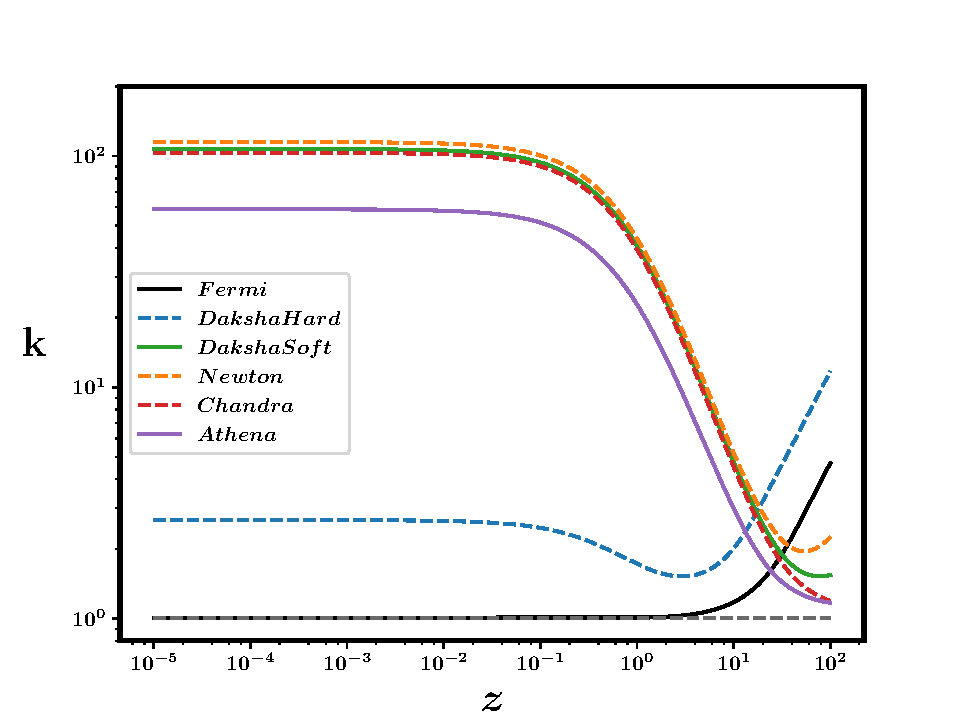
\includegraphics[scale=0.5]{k_correction--long--soft_Xray_instruments_and_Dakshas}
\caption[$k(z)$ of several GRB detectors]{$k(z)$ for the different soft X-ray instruments -- current, in-line, and proposed -- along with the proposed hard X-ray detector on-board \emph{Daksha}. The \emph{Fermi}-GBM curve is drawn for a reference, along with an ``ideal'' instrument [dashed grey line] that has unit k-correction for all instruments.}
\label{fig:k_corrections_for_long_GRBs}
\end{center}
\end{figure}


\subsection{\D}
\label{subsec:predictions_for_Daksha--long}
This instrument has been proposed by Professor Varun Bhalerao of the Indian Institute of Technology [IIT], Bombay, India. It is currently in the planning phase. It will have a soft X-ray detector operating in the energy range of $1$-$10$ keV, in addition to a hard X-ray detector sensitive to $20$-$200$ keV. The sensitivity for both the instruments are shown in Figure \ref{fig:sensitivity_plots_for_soft_and_hard_instruments} \eR, as well as given in Table \ref{tab:predictions_for_Daksha--long}, along with the predictions of the LGRB detection rate combined for the BPL and ECPL models, including uncertainties.

\begin{table}[!htbp]
\caption[Specifications and long GRB detections estimates for \D]{The wavelength-coverage and sensitivities of the two instruments on \D\ for typical LGRBs, and predictions of their detection rates combining the BPL and ECPL models and including uncertainties for both the models.}
\label{tab:predictions_for_Daksha--long}
\begin{center}
\begin{tabular}{|c|c|c|}
\hline 
Wavelength range & Sensitivity & Predicted numbers\\
{[keV]} & [$\ergpercmsqpersec$] & [$\py$]\\
\hline
\hline
$1$-$10$ & $0.3 \times 10^{-8}$ & $210$-$246$\\
\hline
$20$-$200$ & $1.7 \times 10^{-8}$ & $229$-$274$\\
\hline
\end{tabular}
\end{center}
\end{table}

The primary reason that the numbers for the soft X-ray instrument for \D\ are not as low as that of \X, \C, and \A, is its comparatively much larger FoV, technically the full-sky. Corrected for the SAA-passage [equatorial orbit] and earth occultations [low-earth orbit, like \AS], it is $\frac{\Delta \Omega}{4\pi} \sim \frac{1}{2}$. The luminosity distributions for the ECPL model are shown in Figure \ref{fig:N(L)_for_soft_Xray_instruments}, \eR.

\begin{checkit}
This investigation was carried out in collaboration with Professor Varun Bhalerao of the Indian Institute of Technology [IIT], Bombay, India, and the results were communicated to him along with the details.
\end{checkit}





\section{Prospect of TDE science with \A-WFI}
\label{sec:prospects}
Driven by the negative prospects of observing GRBs with \A -WFI [see Section \ref{subsec:predictions_for_soft_Xray_instruments--long}], we ask the following question instead: What is the prospect of \A -WFI to observe Tidal Disruption Events [TDEs]?

We first note that there are many issues with TDE science:
\begin{enumerate}
\item It is difficult to identify TDEs. In the optical wavelengths, it is difficult to distinguish them from supernovae. Even amongst so-called confirmed TDE candidates, there is no uniformity in the slope of the lightcurve [which may vary for a given TDE], or their spectral properties. Subsequently, multiple claims have been made that a certain extragalactic source is a TDE candidate via purely spectral fits, but there is no confirmation as such for these sources. On the other hand, theoretical studies claim that a good fraction of TDEs [$\sim 10 \%$] of AGN activity is due to TDEs; that the TDE-AGN activities span a continuous spectrum than a discrete difference in observables.

\item The intrinsic number of TDEs are much smaller than other transients [like GRBs]: $10^{-5}$-$10^{-4}$ per year per galaxy \citep{Auchettl_et_al.-2018-ApJ}. This is significantly lower than the progenitor mass available for GRBs, for example.
\end{enumerate}

As such, severe instrumental effects are present in the sample of the TDEs themselves. There are around $70$ TDE candidates \citep{Auchettl_et_al.-2017-ApJ}, out of which a significant fraction may not be TDEs. Confirmed TDEs counts is $\sim 20$ in all these years of observation. Here is where an instrument with the probability of detection of $1$ TDE per year may make a significant impact to the TDE science. Roughly, the TDE ``activity'' time is $\sim \frac{1}{3}$ year, so follow-up of the same TDE in different wavelengths, and hence being able to confirm the fact that it is a TDE, is important yet observationally not expensive for such an instrument. Currently, TDEs have been observed either at optical wavelengths, or at soft X-rays. Aside the current optical surveys, a good soft X-ray monitor has the capability of increasing the TDE sample. \emph{MAXI} is a wide-field soft X-ray monitor which has detected 4 TDEs in 37 months of data \citep{Kawamuro_et_al.-2016-PASJ}. Other important instruments have been \s -XRT and the XMM-Newton slew survey. The luminosity function [mathematical definition different from the GRB case, although in the same spirit] has been studied by both \cite{Kawamuro_et_al.-2016-PASJ} and in much more detail by \cite{Auchettl_et_al.-2018-ApJ}. Whereas the former is severely limited by the low statistics of the sample, the latter somewhat alleviates this problem. The selection effects at different luminosities, however, cannot be mitigated. Acknowledging these effects, they have still been able to make some important statements:

\begin{itemize}
\item At $\LX < 10^{44} \, \ergpersec$, the contribution of both jetted and non-jetted TDEs to the AGN LF is significant, specially at low redshifts [$z < 0.4$], in line with theoretical predictions \citep{Milosavljevic_et_al.-2006-ApJ}. However at higher redshifts the contribution becomes less significant.

\item The observed TDE LF has virtually no contribution from the non-jetted TDEs at $\LX > 10^{44} \, \ergpersec$, as also expected theoretically [from the BH mass limit].

\item The observed TDE LF flattens for both the jetted and non-jetted TDEs, thus deviating from the theoretical predictions, for $\LX \sim 10^{40}$-$10^{42} \, \ergpersec$, which is mostly likely an observational artifact. The TDEs supposed to populate this region can be explained by the ``veiled'' TDEs \citep{Auchettl_et_al.-2017-ApJ}.

\item The overall behaviour points to the fact that the observed TDE LFcould very well converge to the theoretical prediction, with future observations. This has an important consequence, as discussed below.
\end{itemize}

The intrinsic TDE source rate derived from the said theoretical study implies a significantly higher rate of stellar disruptions near central supermassive black holes, than those inferred from observations in the optical/UV. This raises another important question: Is the rate of TDEs inferred from optical/UV studies an order of magnitude smaller than those from X-ray observations?

If the above is true, then the prediction for the observable rate for any soft X-ray instrument can increase by a factor of $10$. This is supported by the recent finding of \cite{Tadhunter_et_al.-2017-NatAst}.

Taking all these into account, it can be argued that if a particular instrument can detect and follow-up $1$ TDE $\py$, it can significantly impact the field. Not only that, it can alleviate the instrumental selection effects at the $10^{40}$-$10^{42} \, \ergpersec$ plateau, if sensitive at an energy range that may pick up TDEs with such luminosities. Ideally, one would like a wide-field soft X-ray monitor. A trade-off might be obtained by having an instrument with much better sensitivity but lower FoV. Such an instrument is \A -WFI. It has the potential to significantly impact this field if the number of galaxies it can survey is around $10^3$-$10^4$ times larger than the current instruments.

For focussing instruments on-board \X, \C, \A, the sensitivity scales with time as $t^{-1}$. As for TDEs, the time to be taken for integration is uncertain. But since WFI is an instrument that will not be staring at the same field for months, it is safe to assume that the sensitivity will be maximum two order higher than that for GRBs. Taking into effect the mass and luminosity function of galaxies \citep{Conselice_et_al.-2016-ApJ}, and given that the intrinsic TDE rate is much smaller \citep{Auchettl_et_al.-2018-ApJ}, the number of galaxies available for survey will not be enough for WFI to make any significant stride in this field.

There is another criticism against WFI as a TDE detector: Even though it is going to observe deeply when it its narrow FoV, without having an existing catalogue of the steady sources in that field from a previous survey, it will be impossible to understand whether a given source is a steady source or a transient. This problem does not arise for GRBs because the prompt emission of GRBs are really short [maximum around $100$ s] and extremely significant [at least for LGRBs], but a large number of TDEs are still confused with supernovae as these two classes behave similarly, both temporally and spectroscopically. Only if e-ROSITA can survey deeper than WFI and complete the full-sky catalogue before WFI starts observing, will it be practically possible to pitch WFI as a TDE detector.

\begin{checkit}
The results from this literature survey and basic calculations were communicated to Professor David Burrows and Dr. Pragati Pradhan of the Pennsylvania State University, State College, Pennsylvania, the USA.
\end{checkit}












\section{Conclusions}
\label{sec:conclusions--LGRBs}
Previously, \B\ and \s\ GRBs have been used to constrain the GRB luminosity function. Only a few \B\ GRBs had redshift measurements, so indirect methods were used to study the luminosity function of these GRBs. On the other hand, about $30 \%$ of the \s\ GRBs have redshift measurements. However, the measurement of the spectral parameters are also crucial to the measurement of the luminosity, via the $k$-correction factor. Being limited in the energy coverage, estimates of the \s\ spectral parameters have large uncertainties. Moreover, the number of \s\ GRBs with redshift measures are not as large as the entire \B\ sample. \f\ is a GRB detector with large sky coverage, a detection rate roughly $3$ times more than \s, and wide energy coverage, thus measuring the broad-band spectrum of a large fraction [$\sim 75 \%$] of the detected GRBs to sufficient accuracy. However, its poor localisation capabilities makes it impossible to make \s-like follow up observations, and hence the measurement of redshifts.

In this work, I show that one of the methods proposed to solve the absence of redshift measures for \B\ GRBs can be used self-consistently to estimate the luminosities of \s\ and \f\ GRBs without redshift measurements. This method works on the premise that the `Yonetoku correlation' is applicable to all GRBs. For this, I have first used the most updated common sample of $66$ long GRBs detected by these two instruments, to re-derive the parameters of this correlation. By a careful study of the discrepancies, I find a significant trend between the ratio of the observed and predicted luminosities with the measured redshift. The exact reason for this trend is not clear, but it highlights the fact that the weakness of the correlation is intrinsic, being driven by physical effects and not measurement uncertainties. I conclude that although the large scatter in the Yonetoku correlation rules out the possibility of using GRBs as distance-indicators, the statistical distribution of observed redshifts is reproduced well, and there is no need to modify the extraction of the correlation parameters as has been suggested previously \citepalias{Tan_et_al.-2013-ApJL}.

Next, the method is shown to self-consistently predict `pseudo redshifts' of all long GRBs without redshift measurements. This allows calculation of the luminosities of a total of $2067$ GRBs from these instruments, including the subsample [of $66$ bursts] that has direct measurements of both redshift and spectra. I then use this large sample to model the GRB luminosity function, and place constraints on two models. The GRB formation rate is assumed to be a product of the cosmic star formation rate and a GRB formation efficiency for a given stellar mass. Whereas an exponential cut-off powerlaw model does not require a cosmological evolution, a broken powerlaw model requires strong cosmological evolution of both the break as well as the GRB formation efficiency [degenerate upto the beaming factor of GRBs]. This is the first time \f\ GRBs have been used independent of measured redshifts from \s\ to study the long GRB luminosity function. Moreover, this is the first time such a large sample of \s\ GRBs have been used. The use of the large sample of \f\ GRBs helps in placing sufficient confidence on the derived parameters of the broken powerlaw model, when \s\ GRBs alone suffer from degeneracies and observational biases. Comparison with recent studies shows reasonable agreement for both the models, however it is not possible to distinguish between them.

\citetalias{Amaral-Rogers_et_al.-2017-MNRAS} has proposed on increasing the sample of LGRBs by taking individual pulses of the same bursts as physically separate entities. In the future, perhaps a conglomeration of their method with the one here can be implemented to increase the sample size even further, to further test the parameters of the models and also carry out an in-depth analysis of the detection probabilities of the two instruments, which is presently quite a daunting task. This work also does not attempt to provide a physical understanding of the empirical models or the parameter values derived, which should be addressed in future works.

Finally, I have used the derived models as templates to make predictions about the detection rate of long GRBs by various instruments. The predictions for \AS -CZTI are encouraging for the ongoing efforts of the collaboration. The quick localisation of the few bursts that are predicted to be detected only by CZTI can increase the GRB database even further, and reveal interesting answers about the GRB phenomenon in both the local and the distant universe. The Indian mission \D\ also has great prospects as a GRB-detector. However, the scenario is not bright for past, present and even future soft X-ray [$< 15$ keV] telescopes, even with the improvement of sensitivity. The reason for that is simple: there are just not enough GRBs which peak at such soft energies. As an extension, the prospects of \A -WFI, a future soft X-ray detector, as a detector of tidal disruption events is also considered, and the results are not promising.

\chapter{Luminosity function of short GRBs}
\label{chap:SGRBs}
\begin{checkit}
This work is based on \cite{Paul-2018-MNRAS--short}. I sincerely thank Professor A R Rao for providing the motivation for the work; Professor Patrick Dasgupta for discussions on GRBs throughout the course of the work; \AS -CZTI member Vidushi Sharma for the updated list of GRBs detected by CZTI and related discussions; Professor Varun Bhalerao, Marek J. Szczepanczyk and Shreya Anand for discussions on the aLIGO/VIRGO sensitivities; Muhammad Saleem for providing simulations of BNSM detections with GW detectors at their designed sensitivities; and the anonymous referee for the critical comments that significantly improved the quality of the work.
\end{checkit}



\section{Introduction}
\label{sec:introduction--SGRBs}
The observed rate of SGRBs by a GRB-monitor depends on three criterion: (1) the true event rate of SGRBs as a function of intrinsic properties of the population: the redshift and luminosity; (2) the beaming factor of the SGRBs [since GRBs are powered by relativistic jets, the relativistic beaming of the emission reduces the observed rate from the true event rate]; and (3) the observation windows [e.g. mission time, field-of-view] and detection criteria of the GRB monitor. By modelling the intrinsic distribution of the population of SGRBs, one can infer the true event rate of the population, and its possible cosmological evolution.

Several authors have sometimes modelled different observational entities to estimate the true event rate, at other times used different models for the same entity, and most obviously, different databases. For example, \cite{Guetta_and_Piran-2005-A&A} [hereafter \citetalias{Guetta_and_Piran-2005-A&A}], \cite{Guetta_and_Piran-2006-A&A} [hereafter \citetalias{Guetta_and_Piran-2006-A&A}] and \cite{Salvaterra_et_al.-2008-MNRAS} have modelled the observed peak flux distribution of the GRBs detected by the \emph{Compton Gamma Ray Observatory [CGRO]}-\B\, while \cite{Hopman_et_al.-2006-ApJ}, \cite{Guetta_and_Stella-2009-A&A}, \cite{Dietz-2011-A&A} and \cite{Petrillo_et_al.-2013-ApJ} have modelled the distribution of observed redshifts. The latter approach may be severely affected by the detection of only a handful of bursts with redshifts measurements, with the measurement of the redshifts itself being biased towards smaller values via the identification of host galaxies. Such selection biases have been studied and alternative approaches proposed by \cite{D'Avanzo_et_al.-2014-MNRAS} [hereafter \citetalias{D'Avanzo_et_al.-2014-MNRAS}]. On the other hand, \cite{Virgili_et_al.-2011-ApJ} have attempted to fit the peak-flux distribution of both \B\ and \s\ \citep{Barthelmy_et_al.-2005-SSRv-SwiftBAT,Gehrels_et_al.-2004-ApJ} bursts, as well as the observed redshift distribution, while \cite{Wanderman_and_Piran-2015-MNRAS} have used the peak-flux distribution of \B, \s\ and \f -GBM \citep{FermiGBM-2009-ApJ} bursts along with the redshifts distribution. Subsequently, different authors have placed different constraints on the true event rate. While \citetalias{Guetta_and_Piran-2005-A&A} reported the rate in the local universe, $\Rdot(0)$, to be $0.1$-$0.8 \, \pyG$, \citetalias{Guetta_and_Piran-2006-A&A} extended it to be $8$-$ 30 \, \pyG$ with the addition of \s\ and HETE II bursts, and \cite{Coward_et_al.-2012-MNRAS} [hereafter \citetalias{Coward_et_al.-2012-MNRAS}] at $5$-$13 \, \pyG$ from \s\ bursts alone. On the other hand, \cite{Salvaterra_et_al.-2008-MNRAS}, \cite{Virgili_et_al.-2011-ApJ} and \cite{Wanderman_and_Piran-2015-MNRAS} have claimed that progenitors other than compact object mergers are required to model the detected distributions.

The direct modelling of the LF via the luminosity distribution suffers from the fact there are too few GRBs with observed redshifts and hence estimated luminosities, moreover the sample can suffer from heavy selection bias for the redshift measurement. Although \citetalias{D'Avanzo_et_al.-2014-MNRAS} suggested a method of eliminating the selection bias by limiting to a `flux-complete' sample, the number of bursts thus obtained is too low to make direct modelling of the LF meaningful. To get around this problem, the method suggested originally for LGRBs by \citetalias{Yonetoku_et_al.-2004-ApJ} and discussed extensively in Chapter \ref{chap:LGRBs}, was extended by \cite{Yonetoku_et_al.-2014-ApJ}  [hereafter \citetalias{Yonetoku_et_al.-2014-ApJ}] on SGRBs, using the so-called `Yonetoku correlation' found by \cite{Tsutsui_et_al.-2013-MNRAS} [hereafter \citetalias{Tsutsui_et_al.-2013-MNRAS}] for eight SGRBs. They used $72$ \B\ SGRBs whose spectra were modelled by the Band function, concluding that the LF is consistent with a simple powerlaw with an index of unity, and $\Rdot(0)$ in the range $0.24$-$0.94 \, \pyG$.

\cite{Ghirlanda_et_al.-2016-A&A} [hereafter \citetalias{Ghirlanda_et_al.-2016-A&A}] did an extensive study of the distributions of four observed parameters of \s\ and \f\ bursts, namely the peak flux, fluence, observer frame duration and the observer frame peak energy, and also the distributions of redshift, isotropic energy and isotropic luminosity of a `flux-complete' sample of \s\ bursts presented by \citetalias{D'Avanzo_et_al.-2014-MNRAS}. In doing so, they assumed the validity of the Yonetoku as well as the Amati correlations, whose parameters were included in the model. Contradictory to \citetalias{Yonetoku_et_al.-2014-ApJ}, they concluded that the LF is inconsistent with a simple powerlaw function, and fitted a broken powerlaw with a constant break luminosity, combined with different distributions of the formation rate of the SGRB progenitors. They reported $\Rdot(0) \simeq 0.13$-$0.24 \, \pyG$ and $\Rdot(0) \simeq 0.65$-$1.1 \, \pyG$ for the two fitted models.

In this work, I have applied the method followed by \citetalias{Yonetoku_et_al.-2014-ApJ} to model the luminosity distribution of the full sample of SGRBs detected by \B, \f, and \s\ till October, 2017. This is made possible by using the simplification proposed for LGRBs in Chapter \ref{chap:LGRBs}: instead of modelling the spectra of each individual GRB accurately, they are statistically sampled from the true distribution as observed for \f -GRBs, utilizing the wideband information available for \f -GBM. I have then used the fitted models to calculate the true event rate of the SGRBs, and assuming that they are produced from binary neutron star [henceforth NS] mergers, deduced the rate of electromagnetic counterparts of gravitational wave events to which the GW detectors are sensitive in their different observing phases \citep{Abbott_et_al.-2016-review}. This work simplifies the understanding of the SGRB production scenario significantly over previous works who carry out general numerical studies of all the parameters in the problem. In assuming inputs from the star formation history of the universe and population synthesis models, and  resorting to direct observations wherever applicable [e.g. the Yonetoku correlation data and the \f\ spectral parameter observations], it considerably simplifies the numerical framework and demonstrates that robust statements about the physical scenario can be made nonetheless.

This chapter is organized as follows. The validity of the Yonetoku correlation is investigated in Section \ref{subsec:Yonetoku_correlation--short}, the generation of the luminosity of all SGRBs is described in Section \ref{subsec:L-z_data_generation--short}, the modelling of the LF is detailed in Section \ref{subsec:modelling_LF--short}. In Section \ref{sec:local_SGRB_rate}, the local GRB rate is inferred from the models. In Section \ref{sec:predictions--short}, predictions are made for \AS -CZTI [Section \ref{subsec:predictions_for_CZTI--short}] and \D\ [Section \ref{subsec:predictions_for_Daksha--short}]. The true SGRB rate is derived via the derived models, and extrapolated to derive the BNSM rate, in Section \ref{sec:Events_rate}. In Section \ref{sec:conclusions--SGRBs}, concluding remarks are presented. All the catalogue data, scripts used and important databases generated in this chapter are publicly available at: \url{https://github.com/DebduttaPaul/luminosity_function_of_sGRBs}.


\begin{table}
\caption[Catalogue of short GRBs with both redshift and spectral parameters]{The catalogue of $15$ short GRBs, defined as $\T < 2.0$ s, with redshift measured from localisation and spectral parameters obtained via long wavelength coverage. The spectral peak given here refers to that in the source frame. The data are taken from: [1] \citetalias{Tsutsui_et_al.-2013-MNRAS}, [2] \citetalias{Paul-2018-MNRAS--long}, [3] \citetalias{D'Avanzo_et_al.-2014-MNRAS}, see references therein for the GCNs reporting the individual discovery and follow-ups.}
\label{tab:short_catalogue}
\begin{center}
\begin{tabular}{|c|c|c|c|c|c|}
\hline
GRB name & $\T$ & $z$ & $\Eps$ & $\Lp$ & reference \\
 & [s] &  & [keV] & [$10^{50} \, \ergpersec$] & \\
\hline
\hline
040924 & $1.51$ & $0.86$ & ${124.55}^{+11.15}_{-11.15}$ & $228^{+25}_{-24}$ & 1 \\
\hline
050709 & $0.70$ & $0.16$ & ${97.32}^{+7.76}_{-0.58}$ & $7.51^{+0.76}_{-0.81}$ & 1 \\
\hline
051221A & $1.41$ & $0.55$ & ${621.69}^{+87.42}_{-67.69}$ & $277^{+29}_{-29}$ & 1 \\
\hline
061006 & $0.50$ & $0.44$ & ${954.63}^{+198.39}_{-125.86}$ & $206^{+15}_{-31}$ & 1 \\
\hline
070714B & $2.00$ & $0.92$ & ${2150.40}^{+910.39}_{-443.52}$ & $656^{+79}_{-136}$ & 1 \\
\hline
080905A & $0.96$ & $0.12$ & ${759.30}^{+308.28}_{-308.28}$ & $1.02^{+1.02}_{-1.02}$ & 2 \\
\hline
090510 & $0.30$ & $0.90$ & ${8679.58}^{+947.69}_{-947.69}$ & $10400^{+2400}_{-1400}$ & 1 \\
\hline
100117A & $0.31$ & $0.92$ & ${936.96}^{+297.6}_{-297.6}$ & $189^{+21}_{-35}$ & 1 \\
\hline
100206 & $0.13$ & $0.41$ & ${638.98}^{+131.21}_{-131.21}$ & $99.8^{+115.0}_{-32.5}$ & 1 \\
\hline
100625A & $0.32$ & $0.45$ & ${701.32}^{+114.71}_{-114.71}$ & $34^{+1}_{-1}$ & 3 \\
\hline
100816A & $2.00$ & $0.81$ & ${235.36}^{+15.74}_{-15.74}$ & $96.9^{+19.5}_{-12.8}$ & 1 \\
\hline
101219A & $0.60$ & $0.72$ & ${841.82}^{+107.56}_{-82.50}$ & $156^{+24}_{-23}$ & 1 \\
\hline
111117A & $0.46$ & $1.30$ & ${966.00}^{+322.00}_{-322.00}$ & $404^{+128}_{-128}$ & 3 \\
\hline
130603B & $0.09$ & $0.36$ & ${894.96}^{+135.60}_{-135.60}$ & $435^{+87}_{-87}$ & 3 \\
\hline
131004A & $1.15$ & $0.72$ & ${247.22}^{+153.72}_{-153.72}$ & $23.73^{+23.73}_{-23.73}$ & 2 \\
\hline
\end{tabular}
\end{center}
\end{table}

\begin{figure}
\begin{center}
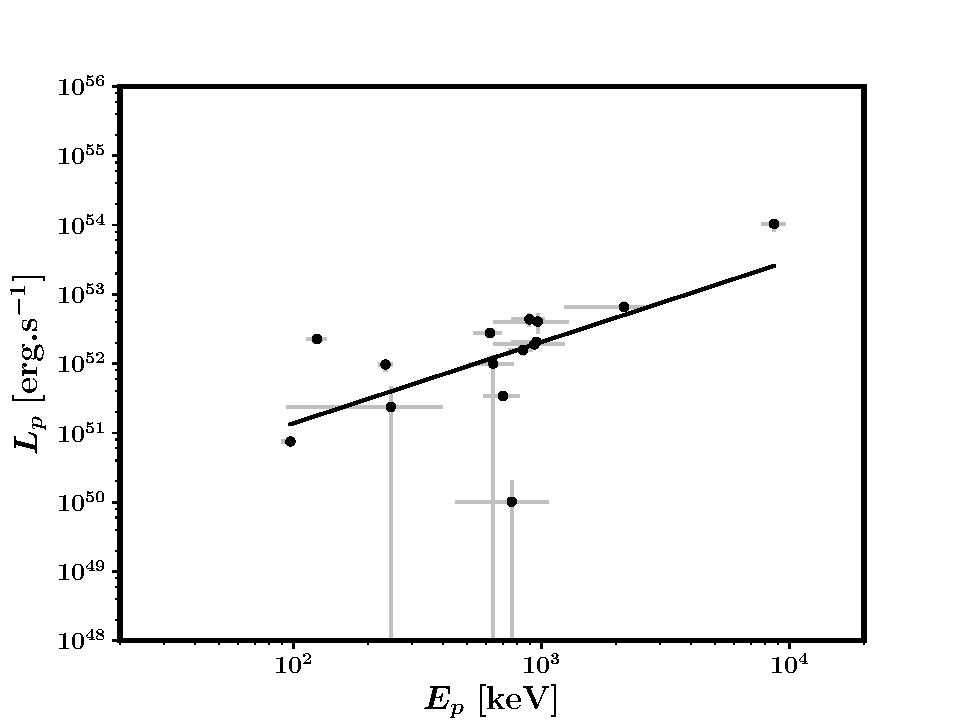
\includegraphics[scale=0.5]{L_vs_Ep0--correlations}
\caption[Yonetoku correlation for short GRBs]{The Yonetoku correlation as seen from the data of $15$ short GRBs with spectral parameters as well as redshift measurement, given in Table \ref{tab:short_catalogue}. $A = 2.04 \pm 0.22$ and $\eta = 1.17 \pm 0.18$ corresponding to Equation \ref{eq:Yonetoku_correlation--long} shows the best fit as the black solid line.}
\label{fig:Yonetoku_correlation--short}
\end{center}
\end{figure}


\section{The luminosity function}
\label{sec:luminosity_function--short}

\subsection{The Yonetoku correlation}
\label{subsec:Yonetoku_correlation--short}
The validity of the Yonetoku correlation [Equation \ref{eq:Yonetoku_correlation--long}] is first tested by combining all data from existing literature. The short GRBs are defined as $\T < 2.0$ s, instead of using the duration in the rest frame \citepalias{Tsutsui_et_al.-2013-MNRAS}. This is to be consistent with the general convention followed in the rest of the work, where the full sample without the redshift information are used, making it impossible to classify bursts using only the source-frame criterion. Using this criterion, $15$ GRBs with redshift measured from ground-based follow-ups, and spectral parameters from long-wavelength coverage, are found in the literature: given in Table \ref{tab:short_catalogue} and plotted on the Yonetoku space in Figure \ref{fig:Yonetoku_correlation--short}. Although the number of sources is small and there are at least three outliers, the correlation is found to be significant: a linear correlation coefficient of $0.98$ is retrieved, and the hypothesis that it is generated from a random distribution is discarded [a probability of $8.9 \times 10^{-11}$]. This also justifies that the effect of outliers on the correlation is not significant, hence possible contamination of the sample by long GRBs, or the effect of missing out a few short GRBs with longer durations in the observer's frame \citep{Zhang_et_al.-2009-ApJ} does not have any effect on the rest of the work.

The best fit to the linear correlation is given by Equation \ref{eq:Yonetoku_correlation--long}, with $A = 2.04 \pm 0.22$ and $\eta = 1.17 \pm 0.18$. The parameters obtained by \citetalias{Tsutsui_et_al.-2013-MNRAS}, with the presently-defined normalization, are given by $A = 2.93^{+0.57}_{-0.48}$ and $\eta = 1.59 \pm 0.11$. The results are thus not significantly different, as expected from the fact that the current database includes and extends their dataset.



\subsection{Generating the luminosity data}
\label{subsec:L-z_data_generation--short}
To model the LF of SGRBs, their luminosities are required for a large sample. In this work, the Yonetoku method of estimating luminosities via the pseudo-redshifts from the Yonetoku correlation is extended to include all SGRBs available in the catalogues of \emph{CGRO}-\B\ \citep{BATSE_catalogue--1997}\footnote{\url{https://heasarc.gsfc.nasa.gov/W3Browse/all/batsegrb.html}}, \s -BAT\footnote{\url{https://swift.gsfc.nasa.gov/archive/grb_table/}}, and \f -GBM \citep{Fermi_catalgoue--2016-ApJS}\footnote{\url{https://heasarc.gsfc.nasa.gov/W3Browse/fermi/fermigbrst.html}}. As before, the distinction between the short and long bursts is drawn at $\lessgtr 2$ seconds, and a total of $757$ GRBs are thus available up to GRB171025913 [\f\ nomenclature].

Since the operational time of \B\ and the later missions are mutually exclusive, there is no \B\ GRB that is coincident with \s\ and \f. However, the latter two missions do have a small but significant number of coincidence, see Chapter \ref{chap:LGRBs}, and the same method is followed for identifying them. As before, all bursts which are detected by both the instruments but do not have redshift measurements, are treated as \f\ GRBs and included in the \f\ dataset for the modelling, i.e. the corresponding $k(z)$ [see below] and $L_c (z)$ are used. For the exclusively \f -bursts, the ones with spectral parameters available in the catalogue are referred to as Type I, while the ones without them as Type II. For the latter, pseudo redshifts are generated similar to that of all other \B\ and \s\ bursts. The number of bursts thus available for generating pseudo redshifts are given in Table \ref{tab:pseudo_numbers--short}. The total number of \s\ bursts with available redshifts, with or without spectral parameters and including those in Table \ref{tab:short_catalogue}, is $30$. Since the modelling for each mission needs to be carried out separately due to the difference in $L_c (z)$ [see Equation \ref{eq:definition_of_phi}], the total number available for each mission for this purpose are given separately in Table \ref{tab:GRBs_used_for_modelling_LF--short}.

\begin{table}
\caption[Categories of short GRBs with pseudo redshift]{The number of SGRBs for which pseudo-redshifts are estimated, for each mission. For both \B\ and \s, the spectral parameters are not available in the catalogues. The \f\ catalogue however contains SGRBs with both Band function parameters estimated, and otherwise; the classification of \f -bursts is explained in Section \ref{subsec:L-z_data_generation--short} and are plotted separately in Figure \ref{fig:L-z--short}.}
\label{tab:pseudo_numbers--short}
\begin{center}
\begin{tabular}{|c|c|c|}
\hline 
mission & spectral parameters available & number \\
\hline 
\hline 
\B &  no & $468$ \\
\hline 
\multirow{2}{*}{\f} & yes, Type I & $188$ \\
\cline{2-3} 
 & no, Type II & $21$ \\
\hline 
\s &  no & $59$ \\
\hline
\hline
TOTAL & & $736$ \\
\hline
\end{tabular}
\end{center}
\end{table}

\begin{table}
\caption[Categories of short GRBs used for modelling LF]{The number of SGRBs available for each mission. See Table \ref{tab:pseudo_numbers--short} for the classification of GRBs with pseudo redshifts. The nomenclature here also corresponds to the $k$-correction used for the calculation of the luminosities as well as the selection thresholds, $L_{c} (z)$ [Equation \ref{eq:definition_of_phi} and Figure \ref{fig:L-z--short}].
\label{tab:GRBs_used_for_modelling_LF--short}}
\begin{center}
\begin{tabular}{|c|c|c|}
\hline
mission & redshift & number \\
\hline
\hline
\B &  pseudo & $468$ \\
\hline
\multirow{2}{*}{\f} & pseudo & $209$ \\
\cline{2-3} 
 & measured & $2$ \\
\hline
\multirow{2}{*}{\s} & pseudo & $59$ \\
\cline{2-3}
 & measured & $19$ \\
\hline
\hline
TOTAL & & $757$ \\
\hline
\end{tabular}
\end{center}
\end{table}


\begin{figure}
\begin{center}
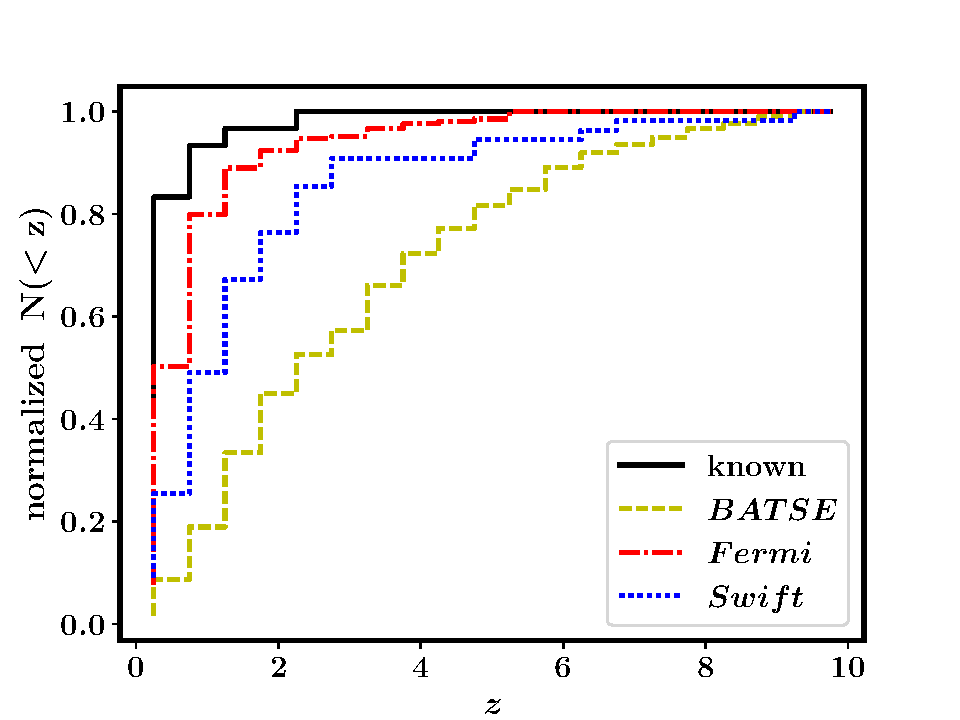
\includegraphics[scale=0.42]{redshift_distributions--cumulative}
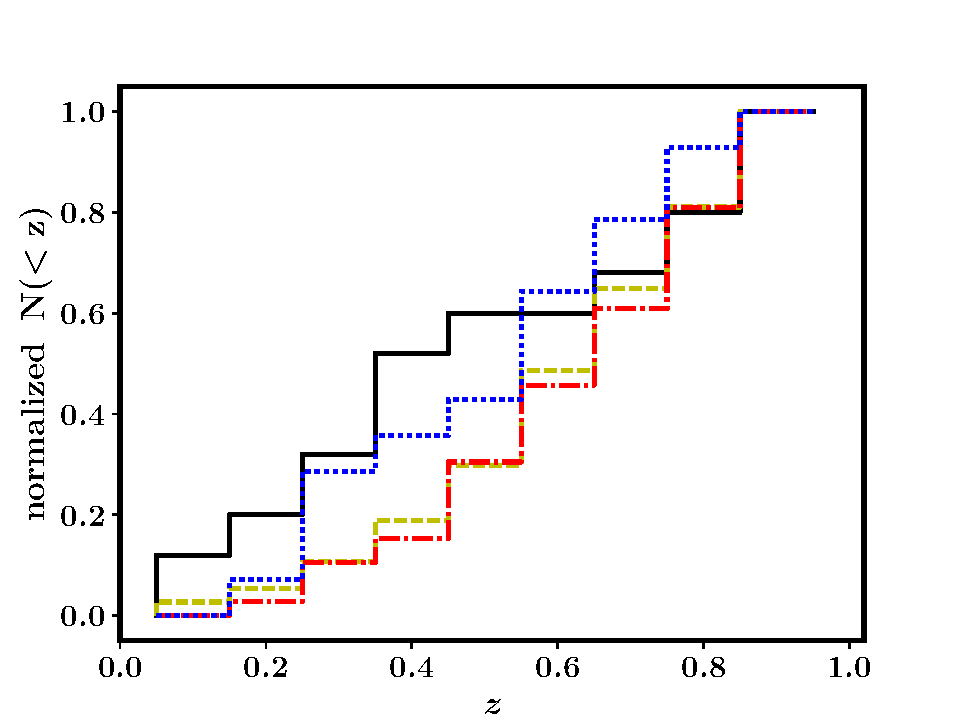
\includegraphics[scale=0.42]{redshift_distributions--cumulative--truncated}
\caption[Cumulative distribution of measured and pseudo redshifts]{The cumulative distribution of redshifts. The distribution from the $30$ GRBs with known redshifts, including the $15$ given in Table \ref{tab:short_catalogue}, is plotted in black. The pseudo redshifts derived for \B, \f\ and \s\ GRBs are shown in [yellow] dashed,  [red] dot-dashed and [blue] dotted lines respectively. \eL: The full range used for modelling the luminosity function. The 2-sample KS test rules out the hypothesis that the pseudo redshifts are derived from the same distribution as that of the known redshifts. However, the number of GRBs with known redshifts being very small [$30$], this may be due to the instrumental selection effect in redshift measurement. \eR: The same distribution truncated at a redshift of $1.0$, below which $25$ of the GRBs with measured redshifts are located. The KS test cannot rule out that all the curves are drawn from the same distribution up to at least this redshift, upto a high degree of confidence.}
\label{fig:z_distribution--short}
\end{center}
\end{figure}


\cite{Bromberg_et_al.-2013-ApJ} has pointed out that $\lessgtr 0.8$ seconds is a better classifier for \s\ GRBs, and \cite{Wanderman_and_Piran-2015-MNRAS} has supported this claim from their independent study. To estimate the effect of using this classification scheme for \s\ GRBs used in this work, I have carried out the generation of the pseudo redshifts and estimated the corresponding luminosity distribution [see below] for both the \s\ and \f\ GRBs, similar to the data plotted in Figure \ref{fig:data-vs-model}. Executing the 2-sample KS-test on the two luminosity datasets thus generated for each of \s\ and \f\ separately, it is observed that a probability of them being drawn from the same sample is very close to unity [upto nine places after the decimal] in both cases. Hence, the different classification scheme has no bearing on the modelling of the LF and the conclusions about the event rate of SGRBs and BNSMs. This is an advantage of using a method that is only reliable in the statistical sense, as discussed below.


\begin{figure}
\begin{center}
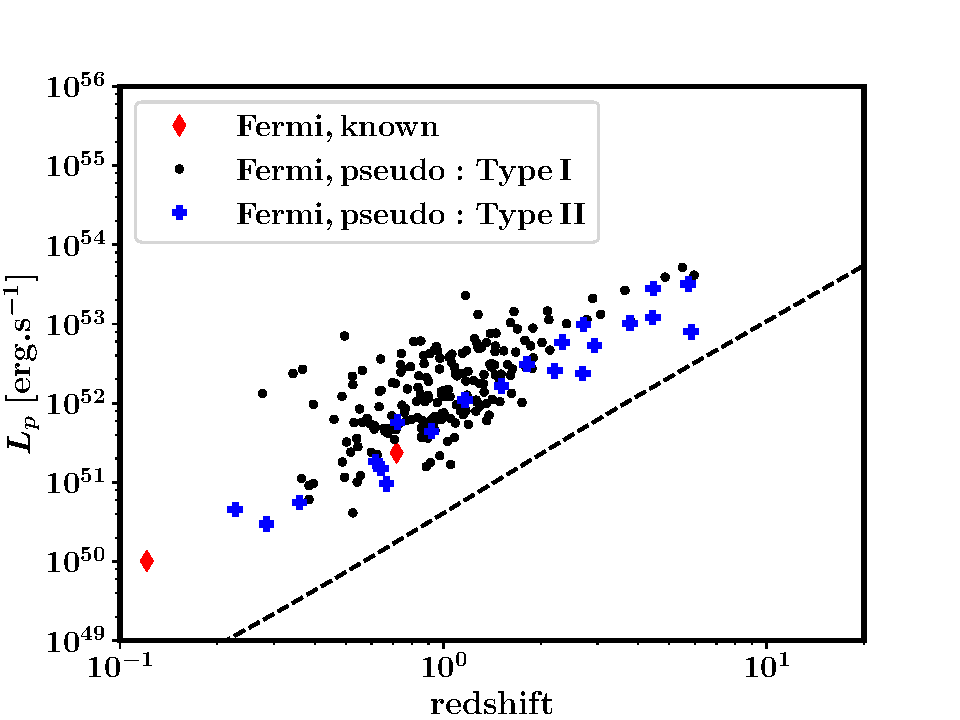
\includegraphics[scale=0.42]{L_vs_z--Fermi_short_all}
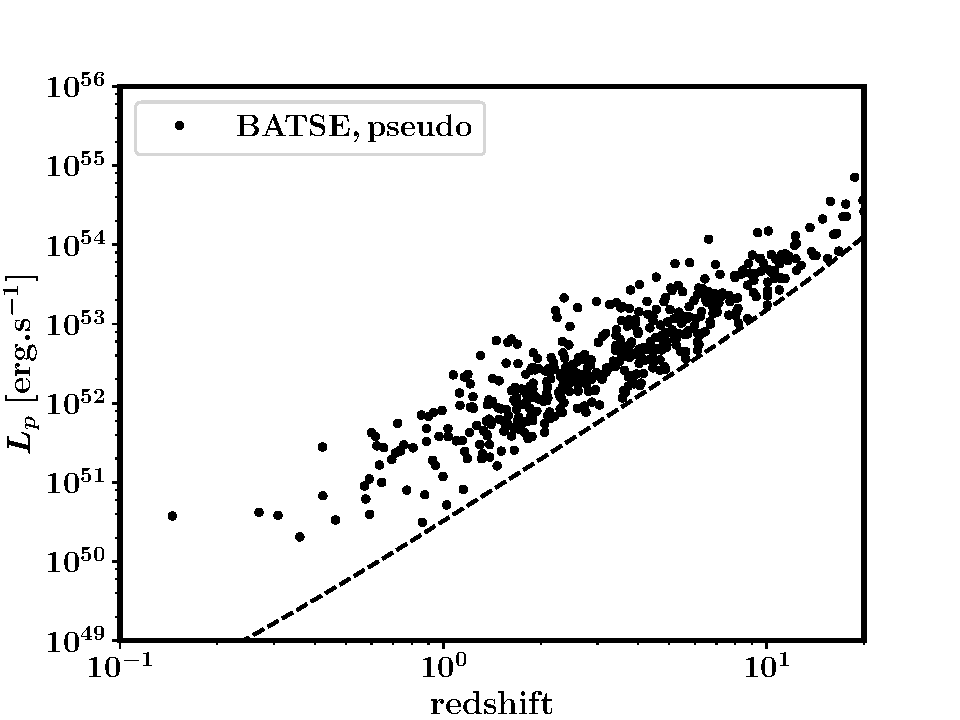
\includegraphics[scale=0.42]{L_vs_z--BATSE_short_all}
\caption[Luminosity versus redshift of all short GRBs]{The $L$-$z$ distributions. The dashed curves give the instrumental sensitivity limits, $L_c (z)$ for the respective instruments, see text below Equation \ref{eq:definition_of_phi}. \eL: For \f; in red [diamond] are the two GRBs with redshift measurement from \s, in [black] dot and [blue] plus are those with pseudo redshifts measured from the Yonetoku correlation, with [Type I, black-dot] and without [Type II, blue-plus] spectral parameters available in the \f\ catalogue [see Section \ref{subsec:L-z_data_generation--short} for the classification and Table \ref{tab:pseudo_numbers--short} for the corresponding numbers]. \eR: Pseudo-redshifts estimated for all \B\ GRBs.}
\label{fig:L-z--short}
\end{center}
\end{figure}



For all GRBs for which spectral parameter measurements are not available, the spectral energy peak $\Ep$ is randomly sampled from that of the observed distribution of \f\ GRBs with spectral measurements, following the example set by LGRBs in Chapter \ref{chap:LGRBs}. The sample of \f\ bursts are again found to have a log-normal distribution of $\Ep$, with $<\Ep> = 382.8$ keV; moreover, $<\alpha> = -0.2$ and $<\beta> = -3.5$. The justification behind this is the same as in the case of LGRBs: \f -GBM being a wide-band GRB detector, samples the $\Ep$ space without any selection bias. This is evident from the fact that the $k(z)$ for \f\ deviates significantly from unity only at very high redshifts [Figure \ref{fig:k-correction--long}] where the formation rate of GRBs is itself extremely low due to the absence of the progenitors. Hence, the spectral parameter distribution of \f -GRBs is representative of the true GRB population. By randomly selecting $\Ep$ from the observed distribution of \f\ bursts, the true distribution of $\Ep$ of bursts is being sampled, and there is no need to additionally model this distribution. In doing so, no claim to the accuracy of the individual values of $\Ep$ is claimed, and hence neither in the individual values of pseudo-redshifts. This approach thus assigns pseudo-redshifts to bursts only in the statistical sense. This limitation is however not binding to this work, since luminosities of the bursts estimated from these pseudo-redshifts are used only as a collective sample in modelling the LF.

The number of SGRBs with known redshift and spectral parameters is only $15$. Hence, to test the hypothesis that the estimated pseudo-redshifts are indeed representative of the whole sample, I compare the cumulative distribution of the pseudo-redshifts thus derived for each of the instruments to that of the measured redshifts of a total of $30$ SGRBs, with or without spectral parameters. The 2-sample KS test rules out the hypothesis that any of the pseudo-redshift distributions are drawn from the known redshift population when the full range of redshifts is considered, as shown in the left panel of Figure \ref{fig:z_distribution--short}. However, the number of GRBs with observed redshifts is still quite small to draw negative conclusions from this global comparison. The discrepancy can be understood to be due to instrumental selection effects that severely limit the detection of GRBs with high redshifts, primarily via the identification of the host galaxy \citep{Berger-2014-sGRB_review}. \citetalias{Yonetoku_et_al.-2014-ApJ} pointed out that the pseudo-redshift distributions matches well with the measured ones from their sample, when both are limited to a redshift of $1.0$. In this work it is found that as many as $25$ of the $30$ GRBs are located within this redshift. Given that the progenitor mass available for the production of SGRBs does not reduce drastically at $z > 1.0$ from population synthesis studies [see Figure \ref{fig:CSFR--short} and Section \ref{subsec:modelling_LF--short}], this is indicative of the fact that selection effects indeed play an important role in the measurement of redshifts of GRBs. When limited to this range, the pseudo-redshift distributions of all the instruments have probabilities $> 0.66$ of being drawn from the same population as the known redshift distribution, see right panel of Figure \ref{fig:z_distribution--short}. Hence the pseudo-redshifts can be safely used to calculate the luminosities for all the bursts with unknown redshifts. The resultant $L$-$z$ distributions of \f\ and \B\ GRBs are shown in Figure \ref{fig:L-z--short}. This approach mitigates the statistical limitation of a sample of redshift-measured bursts, and also the selection bias that plagues the very measurement of redshift. It is to be noted that studies that model the luminosity function considering only the short bursts with measured redshifts, are hence not representative of the true sample.


\subsection{Modelling the luminosity function}
\label{subsec:modelling_LF--short}

\begin{figure}
\begin{center}
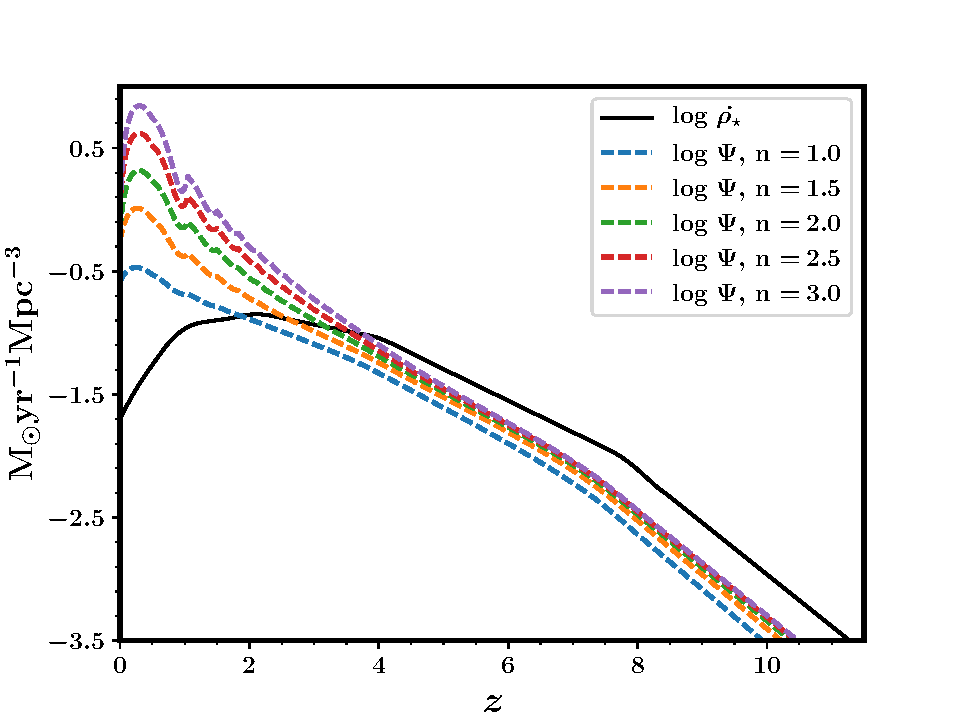
\includegraphics[scale=0.5]{CSFR_delay}
\caption[The binary coalescence rate]{The cosmic star formation rate taken from \citetalias{Bouwens_et_al.-2015-ApJ}, shown in the black solid line, is convolved with a time-delay distribution [see text] via Equation \ref{eq:CSFR_convolution} to derive the binary coalescence rate for various values of the parameter $n$.}
\label{fig:CSFR--short}
\end{center}
\end{figure}


If the SGRB progenitors are produced by coalescences of neutron star [NS] binaries, then assuming that $\Psi(z)$ is the effective mass available for coalescence per unit time per unit volume, it follows the cosmic star formation rate $\csfr(z)$, delayed by a time $\tau$ given by $\tau[z,z'] = t_{\rm{age}}(z) - t_{\rm{age}}(z')$, where $t_{\rm{age}}(z)$ is the age of the universe calculated in the standard way in $\Lambda$-cold dark matter cosmology. If the delay distribution is given by $P(\tau)$, then $\Psi(z)$ at redshift $z$ is given by 
\begin{equation}
\Psi(z) = \intop_{z_{\rm{min}}(z)}^{\infty} \csfr(z') \, P\left( \tau[z,z'] \right) \frac{\dd \tau}{\dd z'} \dd z',
\label{eq:CSFR_convolution}
\end{equation} where $z_{\rm{min}}(z)$ is obtained on solving $t_{\rm{age}}(z) - t_{\rm{age}}(z_{\rm{min}}) = \tau_{\rm{min}}$. The probability distribution function $P(\tau)$ is normalized over the chosen range of $\tau$, bounded below by $\tau_{\rm{min}}$.

$\Psi(z)$ is shown in Figure \ref{fig:CSFR--short} by convolving the cosmic star formation rate obtained from \citetalias{Bouwens_et_al.-2015-ApJ} with a delay distribution of the form $ P(\tau) \propto \tau^{-n}$, for various values of $n$. A number of population synthesis codes \citep{Schneider_et_al.-2001-MNRAS, Belczynski_et_al.-2006-ApJ, O'Shaughnessy_et_al.-2008-ApJ} have studied the rate of binary coalescences, concluding that the delay distribution is typically well-approximated as $P(\tau) \propto \tau^{-1}$ with $\tau_{\rm{min}} = 10$ Myr. For the rest of the work, I let $n$ vary between $1$, $1.5$ and $2.0$ for the sake of generality, although the delayed rate is relatively insensitive to this variation [see Figure \ref{fig:CSFR--short}]. Variation in the choice of $\tau_{\rm{min}}$ in the same order of magnitude has no significant effect on the convolved rate, $\Psi(z)$.

Whereas \citetalias{Yonetoku_et_al.-2014-ApJ} used only $72$ \B\ GRBs with spectral parameters that they estimated, as a result of sampling the $\Ep$ from the observed distribution of that of \f, I have a large number of bursts available to model the SGRB LF via the luminosities computed via the pseudo redshifts, as discussed before. This approach allows a range of models to be tested and sufficient confidence be placed on the parameters of the bestfit model. Moreover, the $\Ep$ measurements have been directly used for the \f\ GRBs whenever available, whereas \citetalias{Ghirlanda_et_al.-2016-A&A} has used the Yonetoku correlation to model the \f\ $\Ep$-distribution via the LF. In Figure \ref{fig:data-vs-model} is shown the luminosity distribution of all the GRBs from the three instruments, along with one best-fit model [see below]. The total number of GRBs used for the different instruments are tabulated in Table \ref{tab:GRBs_used_for_modelling_LF--short}.

The model fits are carried out via the standard Levenberg-Marquardt algorithm of minimizing the discrepancy defined as $d^2 = (model - data)^{2}$, available in the \textsc{python} library \textbf{scipy}\footnote{\url{https://docs.scipy.org/doc/scipy/reference/generated/scipy.optimize.curve_fit.html}}.

Attempts are first made to fit a simple powerlaw [SPL] model of the LF, $\Phi_z(L) \propto L^{-\nu}$, with $\nu \in [0.01,10.0]$. Table \ref{tab:SPL_fits--short} lists the reduced chisquared, $\red$, for $10$ degrees of freedom, for the chosen values of $n$. It is clearly seen that this model is ruled out for all three instruments for the whole range of $\nu$ with a high degree of confidence. This rules out the conclusion of \citetalias{Yonetoku_et_al.-2014-ApJ}, who found the LF to be well-described by a simple powerlaw of index $1$, while supporting and extending the conclusion of \citetalias{Ghirlanda_et_al.-2016-A&A}, who ruled out this model with $ \nu > 2.0. $ The large number of GRBs in the present dataset helps in reaching this conclusion.


\begin{table}
\caption[SPL model mismatch]{The best fits to the SPL model and the corresponding reduced chisquared [$\red$], corresponding to $10$ degrees of freedom.}
\label{tab:SPL_fits--short}
\begin{center}
\begin{tabular}{|c|c|c|c|c|}
\hline
$n$ & parameters & \B & \f & \s \\
\hline
\multirow{2}{*}{$1.0$} & $\nu$ & $1.12$ & $1.23$ & $1.37$ \\
 & $\red$ & $233.1$ & $26.5$ & $10.1$ \\
\hline
\multirow{2}{*}{$1.5$} & $\nu$ & $1.10$ & $1.20$ & $1.33$ \\
 & $\red$ & $276.5$ & $35.4$ & $10.9$ \\
\hline
\multirow{2}{*}{$2.0$} & $\nu$ & $1.09$ & $1.18$ & $1.31$ \\
 & $\red$ & $300.6$ & $39.4$ & $11.2$ \\
\hline
\end{tabular}
\end{center}
\end{table}

\begin{table}
\caption[ECPL model fits]{The best fits to the ECPL model and the corresponding reduced chisquared [$\red$], corresponding to $8$ degrees of freedom. Here, $\Lb$ is given in units of $L_{0} = 10^{52} \, \ergpersec$. The best fits to $\nu$ and $\Lb$ are not provided for the three instruments separately since the same values are applicable to all instruments; whereas $\Gamma$ and $\red$ vary with instruments for the same values for $\nu$ and $\Lb$. The errors refer to $1$-$\sigma$ uncertainties.}
\label{tab:ECPL_fits--short}
\begin{center}
\begin{tabular}{|c|c|c|c|c|c|}
\hline
$n$ & parameters &  & \f & \s & \B \\
\hline
\multirow{4}{*}{$1.0$} & $\nu$ & $0.71 ^{+0.05} _{-0.36}$ & & & \\
 & $\Lb$ & $7.42 ^{+7.21} _{-1.96}$ & & & \\
 & $\Gamma$ & & $0.00$ & $0.00$ & $0.41 ^{+0.15} _{-0.12}$ \\
 & $\red$ & & $0.31$ & $0.21$ & $0.75$ \\
\hline
\multirow{4}{*}{$1.5$} & $\nu$ & $0.64 ^{+0.05} _{-0.39}$ & & & \\
 & $\Lb$ & $6.84 ^{+6.73} _{-1.58}$ & & & \\ 
 & $\Gamma$ & & $0.00$ & $0.00$ & $0.38 ^{+0.13} _{-0.10}$ \\
 & $\red$ & & $0.39$ & $0.19$ & $0.82$ \\
\hline
\multirow{4}{*}{$2.0$} & $\nu$ & $0.60 ^{+0.05} _{-0.38}$ & & & \\
 & $\Lb$ & $6.61 ^{+6.09} _{-1.53}$ & & & \\
 & $\Gamma$ & & $0.00$ & $0.00$ & $0.36 ^{+0.12} _{-0.09}$ \\
 & $\red$ & & $0.41$ & $0.19$ & $0.84$ \\
\hline
\end{tabular}
\end{center}
\end{table}

\begin{table}
\caption[BPL model fits]{The best fits to the BPL model and the corresponding reduced chisquared [$\red$], corresponding to $7$ degrees of freedom. Here, $\Lb$ is given in units of $L_{0} = 10^{52}\, \ergpersec$. The best fits to $\nu_1$, $\nu_2$, and $\Lb$ are not provided for the three instruments separately since the same values are applicable to all instruments; whereas $\Gamma$ and $\red$ vary with instruments for the same values for $\nu_1$, $\nu_2$, and $\Lb$. The errors refer to $1$-$\sigma$ uncertainties.}
\label{tab:BPL_fits--short}
\begin{center}
\begin{tabular}{|c|c|c|c|c|c|}
\hline
$n$ & parameters &  & \f & \s & \B \\
\hline
\multirow{5}{*}{$1.0$} & $\nu_1$ & $0.48 ^{+0.22} _{-0.48}$ & & & \\
 & $\nu_2$ & $1.86 ^{+1.08} _{-0.20}$ & & & \\
 & $\Lb$ & $1.52 ^{+1.58} _{-0.67}$ & & & \\
 & $\Gamma$ & & $0.00$ & $0.00$ & $0.17 ^{+0.05} _{-0.05}$ \\
 & $\red$ & & $0.10$ & $0.42$ & $1.09$ \\
\hline
\multirow{5}{*}{$1.5$} & $\nu_1$ & $0.38 ^{+0.23} _{-0.38}$ & & & \\
 & $\nu_2$ & $1.85 ^{+1.04} _{-0.19}$ & & & \\
 & $\Lb$ & $1.46 ^{+1.36} _{-0.62}$ & & & \\ 
 & $\Gamma$ & & $0.00$ & $0.00$ & $0.16 ^{+0.04} _{-0.05}$ \\
 & $\red$ & & $0.10$ & $0.39$ & $1.09$ \\
\hline
\multirow{5}{*}{$2.0$} & $\nu_1$ & $0.34 ^{+0.23} _{-0.34}$ & & & \\
 & $\nu_2$ & $1.85 ^{+1.03} _{-0.19}$ & & & \\
 & $\Lb$ & $1.45 ^{+1.32} _{-0.60}$ & & & \\
 & $\Gamma$ & & $0.00$ & $0.00$ & $0.15 ^{+0.04} _{-0.05}$ \\
 & $\red$ & & $0.10$ & $0.39$ & $1.09$ \\
\hline
\end{tabular}
\end{center}
\end{table}

\begin{figure}
\begin{center}
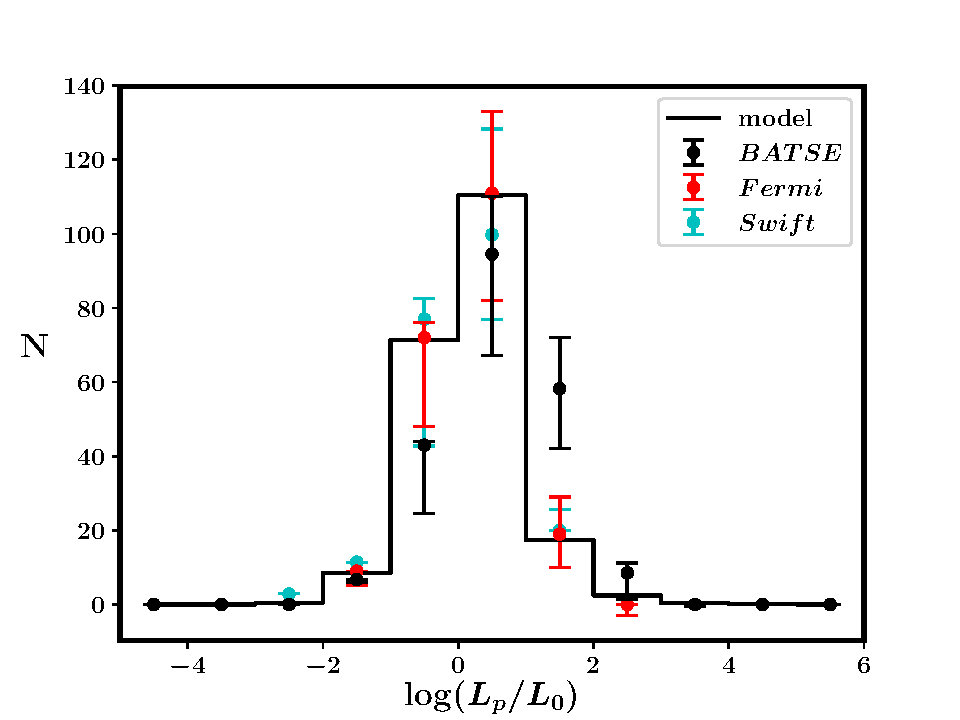
\includegraphics[scale=0.5]{BPL_model--joint--n=1}
\caption[Estimated luminosity distributions and model fit]{The points with error-bars are the data for \B\ [black], \f\ [red] and \s\ [cyan]. It is clearly seen that the \B\ data deviates from the \f\ and \s\ data. The $\Gamma = 0, \; n = 1.0$ BPL model [see Table \ref{tab:BPL_fits--short}] has been plotted as a thick-line, and the bestfit \B\ model with non-zero $\Gamma$ has not been plotted for simplicity. All the plots are normalized to \f; $L_0 = 10^{52} \, \ergpersec$.}
\label{fig:data-vs-model}
\end{center}
\end{figure}


Next, the observed distributions are fit to the ECPL [Equation \ref{eq:The_ECPL_model--long}] and BPL [Equation \ref{eq:The_BPL_model--long}] models. It is seen that, although the \f\ and the \s\ data are well fit by both the models, the \B\ data [see Figure \ref{fig:data-vs-model}] is not. This is clearly understood to be due to the fact that the \B\ data are significantly different from the \f\ and the \s\ data, specially at higher luminosities. While writing Equation \ref{eq:definition_of_phi}, it was assumed that the probability of detection of a burst is $0$ below $L_c$ and $1$ above it. However, that may not be the case for all instruments, the change being gradual. This effect can be modelled by introducing a detection probability that is a function of the observed flux $P$, given as $D(P)$, thus modifying Equation \ref{eq:definition_of_phi} to

\begin{equation}
N(L_1, L_2; z_1, z_2) = T \, \dfrac{\Delta \Omega}{4 \pi} \,
\intop_{z_1}^{z_2} \dd V
\intop_{\rm{max}[L_1,\, L_c]}^{L_2} \dd L \; \Phi_z(L) \dfrac{\Rdot(z)}{1+z} \times D(L, z),
\label{eq:introduction_of_D}
\end{equation} where $D(L, z) \equiv D(P)$. Assuming
\begin{equation}
D(P) \propto P^{\Gamma},
\label{eq:form_of_D}
\end{equation} the normalization is defined such that $ \Phi_z(L) \, D(L,z) $ is normalized in the absolute limits. The data are then fit to the model keeping $\Gamma$ as a free parameter for each instrument. It is envisaged that the same set of parameters for $\Phi_z(L)$ describes the data of each instrument, whereas $\Gamma$ itself may be different for the different instruments. That is indeed the case, with $\Gamma$ being consistent with $0$ for both \f\ and \s, whereas non-zero for the \B\ data.

The combined bestfits to the ECPL and BPL models are given in Tables \ref{tab:ECPL_fits--short} and \ref{tab:BPL_fits--short} respectively. It is seen that the low luminosity index [$\nu_1$] of the BPL model is weakly constrained from below, although the other parameters are well constrained. It is noted that the BPL model fits are consistent with the $68 \%$ confidence intervals quoted for this model by \citetalias{Ghirlanda_et_al.-2016-A&A}, for all three scenarios considered by them. From the current dataset, it is impossible to distinguish between the ECPL and BPL bestfit models, as the relative errors on the luminosity are large due to large propagated errors on the estimated luminosities [$40 \%$ on an average]. Although the break luminosity [$\Lb$] is weakly constrained from above for the ECPL model, the robust lower limits makes it a few times larger as compared to the BPL model, same as in long GRBs \citepalias{Amaral-Rogers_et_al.-2017-MNRAS, Paul-2018-MNRAS--long}.



\section{The local SGRB rate}
\label{sec:local_SGRB_rate}

\begin{table}
\caption[Bestfit normalizations for the models]{The bestfit normalizations for the models. The errors refer to $1$-$\sigma$ uncertainties obtained on propagating the errors in the fitted parameters quoted in Tables \ref{tab:ECPL_fits--short} and \ref{tab:BPL_fits--short}. The range of the local GRB formation rate uncorrected for the beaming factor, $\Rcap(0)$, refers to $68 \%$ confidence limits combining the two models.}
\label{tab:fBC0_fits--short}
\begin{center}
\begin{tabular}{|c|c|c|c|}
\hline 
$n$ & model & $\fB C(0)$ & $\Rdot(0)$ \\
 & & $[10^{-9} \, \Msun^{-1} ]$ & $ [\pyG] $ \\
\hline
\multirow{2}{*}{$1.0$} & ECPL & $13.7 ^{+1.2} _{-3.9}$ & \multirow{2}{*}{$0.68$-$3.89$} \\
 & BPL & $3.74 ^{+3.76} _{-1.15}$ & \\
\hline
\multirow{2}{*}{$1.5$} & ECPL & $6.45 ^{+0.39} _{-1.32}$ & \multirow{2}{*}{$0.82$-$3.80$} \\
 & BPL & $2.05 ^{+1.73} _{-0.58}$ & \\
\hline
\multirow{2}{*}{$2.0$} & ECPL & $3.65 ^{+0.26} _{-0.61}$ & \multirow{2}{*}{$0.61$-$2.66$} \\
 & BPL & $1.23 ^{+0.94} _{-0.34}$ & \\
\hline
\end{tabular}
\end{center}
\end{table}

\begin{table}
\caption[The local short GRB formation rate]{Comparison of the derived local SGRB formation rate uncorrected for the beaming factor, $\Rcap(0)$, with previous works. The rate quoted for the present work combines the results of all considered $n$-s and includes the $68 \%$ confidence intervals of both the models.}
\label{tab:rate_comparison}
\begin{center}
\begin{tabular}{|c|c|}
\hline 
Reference & $\Rdot(0)$ \\
 & $\pyG$ \\
\hline
\hline
G16, model [a] & $0.13$-$0.24$ \\
\hline
GP05 & $0.1$-$0.8$ \\
Y14 & $0.24$-$0.94$ \\
G16, model [c] & $0.65$-$1.10$ \\
present work & $0.61$-$3.89$ \\
\hline
C12 & $5$-$13$ \\
GP06 & $8$-$30$ \\
\hline
\end{tabular}
\end{center}
\end{table}


The normalization of the models are kept free during the fits, and can thus be derived via the solutions. With the knowledge of $T \sim 8.9$ yr and assuming $ \frac{\Delta \Omega}{4 \pi} \sim \frac{1}{3} $ for \f, the ratios of the observed and modelled normalizations [for the corresponding models in Section \ref{subsec:modelling_LF--short}] are converted to derive $\fB C(0)$, which are used to derive the detected SGRB rate via $\Rdot(z) = \fB C(0) \, \Phi(z)$. These, along with the propagated errors, are listed in Table \ref{tab:fBC0_fits--short}, along with the combined $68\%$ confidence intervals of $\Rdot(0)$ combining both the ECPL and BPL models. $\Rdot(z)$ is plotted in Figure \ref{fig:Rdot_of_z--short}, along with those derived by \citetalias{Ghirlanda_et_al.-2016-A&A}. It is seen that this quantity depends only weakly on $n$, as expected. Combining the results, one gets
\begin{equation}
\Rdot(0) = [0.61, 3.89] \, \pyG.
\label{eq:Rdot0--short}
\end{equation}

While clearly higher than model [a] of \citetalias{Ghirlanda_et_al.-2016-A&A}, this is consistent with the higher end of \citetalias{Guetta_and_Piran-2005-A&A}, \citetalias{Yonetoku_et_al.-2014-ApJ} and model [c] of \citetalias{Ghirlanda_et_al.-2016-A&A}, while being smaller than the rates deduced by \citetalias{Guetta_and_Piran-2006-A&A} and \citetalias{Coward_et_al.-2012-MNRAS}. This comparison is summarized in Table \ref{tab:rate_comparison}.


\begin{figure}
\begin{center}
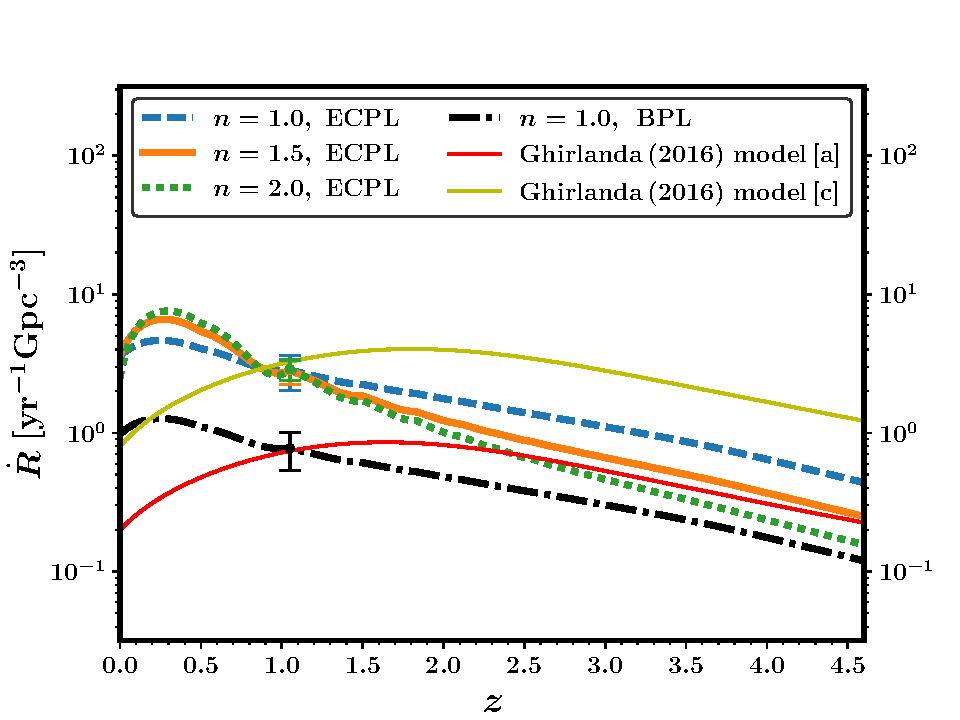
\includegraphics[scale=0.6]{Rdot_of_z}
\caption[The beaming-uncorrected SGRB rate as a function of redshift]{The beaming-uncorrected SGRB rate as a function of redshift, $\Rcap(z)$. The [blue] dashed, [orange] solid and [green] dotted lines correspond to the results from the ECPl model for $n = 1.0$, $1.5$ and $2.0$ respectively. Typical $1$-$\sigma$ errorbars have been shown at a representative redshift $\sim 1$. It is seen that the dependence on $n$ is rather weak. The [black] dot-dashed line represents the $n = 1.0$ BPL model. $\Rcap(0)$ is a few times smaller for the BPL model compared to the ECPL model for each $n$. Since the general dependence with redshift is similar for the two models, only one curve has been shown for the BPL model for simplicity. The red and yellow thick lines represent the model fits from \citetalias{Ghirlanda_et_al.-2016-A&A} [see their Figure 4]. Their $\Rcap(0)$ is smaller compared to the present work [see Table \ref{tab:rate_comparison}]. However, their model-a curve converges with those of the present work at higher redshifts, although model-c is a factor of few higher than the present curves at high redshifts.}
\label{fig:Rdot_of_z--short}
\end{center}
\end{figure}


Comparing Equation \ref{eq:Rdot0--short} to that of Equation \ref{eq:Rdot0--long} for LGRBs [see Section \ref{sec:Modelling_the_GRB_LF--long}], we find that the local GRB formation rate is much larger for short bursts rather than long bursts. Although counter-intuitive given that the rate of detected GRBs is smaller by $\sim 3$ times for SGRBs than LGRBs, the reasons are two-fold: (1) The delay caused by the binary formation and evolution makes most of them merge in the local universe, as compared to the far-away universe, see Figure \ref{fig:CSFR--short}. (2) As demonstrated in Section \ref{subsec:L-z_data_generation--short}, the selection bias in detecting SGRBs at smaller redshifts ensures that we see more SGRBs in the local universe than in the distant universe.


\section{Predictions for \AS-CZTI and \D}
\label{sec:predictions--short}

\subsection{\AS -CZTI}
\label{subsec:predictions_for_CZTI--short}
Combining the model parameters and the derived normalizations, predictions are made for the rate of SGRBs detectable by the \AS\ \citep{Rao_et_al.-2016-arXiv-Astrosat} hard X-ray detector CZTI \citep{Rao_et_al.-2016-ApJ, Bhalerao_et_al.-2017-JApA}, similar to Chapter \ref{chap:LGRBs} where a sizeable under-detection of LGRBs was predicted. Assuming $\frac{\Delta\Omega}{4\pi} \sim \frac{1}{3}$, the combined model rate comes out in the range of $14$-$42$ per year at $68 \%$ confidence. However, in the last two years of operation, it has detected only $11$ SGRBs by triggered searches, i.e. by subjective search of GRBs from automatic triggers by other satellites. Moreover, the searches have been carried out at coarse time-bins due to the uncertainties in the characterization of noise at finer time bins. This study implies that a careful automatic search of the CZTI data post removal of sub-second noise in the data will reveal at least $\sim 20$ SGRBs hidden till date. A careful analysis of the sub-second noise is being carried out and will be reported elsewhere. The importance of an automatic detection algorithm and alerts to the astronomical community for quick follow-up measurements cannot be underestimated.

\subsection{\D}
\label{subsec:predictions_for_Daksha--short}
The predictions of the short GRB detction rates by the \D\ instruments, assuming $\frac{\Delta \Omega}{4\pi} \sim \frac{1}{2}$, are given in Table \ref{tab:predictions_for_Daksha--short}. The prospects look really bright, and if it achieves this expectation and localise the detected SGRBs in real time, it can be game-changer in the emerging field of multi-messenger astronomy. Given the large number of detected sources, sufficient planning is required in advance to prioritise the list of sources that it can do real-time detailed observations of.

\begin{table}
\caption[Specifications and short GRB detections estimates for \D]{The wavelength-coverage and sensitivities of the two instruments on \D\ for typical SGRBs, and predictions of their detection rate combining the BPL and ECPL models but excluding uncertainties [because they are large].}
\label{tab:predictions_for_Daksha--short}
\begin{center}
\begin{tabular}{|c|c|c|}
\hline 
Wavelength range & Sensitivity & Predicted numbers\\
 {[keV]} & [$\ergpercmsqpersec$] & [$\py$]\\
\hline
\hline
$1$-$10$ & $10^{-8}$ & $\sim 11$\\
\hline
$20$-$200$ & $5 \times 10^{-8}$ & $\sim 34$\\
\hline
\end{tabular}
\end{center}
\end{table}



\section{The Binary Coalescence Rate}
\label{sec:Events_rate}
The observed event rate of SGRBs can be corrected for the beaming factor $ \fB = 1 - \cos(\theta_j), $ where $ \theta_j $ is the half-opening angle of the jet, to derive their true sky rate:
\begin{equation}
R_0 = \dfrac{ \Rdot(0) }{\fB}.
\end{equation} Using radio to X-ray afterglow observations of 11 bursts upto 2015, \cite{Fong_et_al.-2015-ApJ} constrained the range of $\theta_j$ to $6$-$26^{\circ}.$ Allowing for the lower limit of the range to be $3^{\circ}$ as derived for GRB111002A \citep{Fong_et_al.-2012-ApJ} and GRB111117A \citep{Margutti_et_al.-2012-ApJ}, the conservative range of $3$-$26^{\circ}$ is used along with $\Rdot(0)$ deduced in the previous section to derive $R_0$. The $68 \%$ confidence ranges are given by $6.72$-$2838 \, \pyG $ for $n = 1.0$; $8.10$-$2773 \, \pyG$ for $n = 1.5$; and $6.03$-$1941 \, \pyG $ for $n = 2.0$. It is to be noted that although the upper limit of $R_0$ is sensitive to the lower limit of $\theta_j$ and hence debatable, the lower limit of $R_0$ depends on the upper limit of $\theta_j$ and is hence fairly robust. Thus, a sharp lower limit of $R_0 \sim 6 \, \pyG$ is placed via this work upto $68 \%$ confidence. Assuming that each BNSM produces a SGRB, this is also the minimum rate of BNSMs; if not, the merger rate is higher.

\cite{Saleem_et_al.-2018-MNRAS} have simulated a large sample of mergers of non-spinning NSs with component masses of $1.4 \Msun$ each, and taking into account the antenna pattern functions of the gravitational wave detectors, calculated the signal-to-noise ratio [SNR] for their detection as a function of the distance to the merger, and inclination of the axis of the merger plane to the line of sight of the observer, $i$. With a detection criterion set to SNR $> 8.0$, this produces the limiting distance [$D_L$] versus inclination [$i$] scatter plot for a combination of detectors: (a) the LH network comprising the Livingston and Hanford detectors, (b) the LHV network with the addition of the Virgo detector, and (c) the LHVKI network, including the KAGRA detector under construction in Japan \citep{Aso_et_al.-2013-PhRvD}, and the approved LIGO-India detector\footnote{\url{https://dcc.ligo.org/LIGO-M1100296/public}} which is expected to come up in the next decade [see their Figure 1 for configurations b and c]. In this work, I have used this simulated dataset and integrated the $68 \%$ lower limit of $\Rdot(z)$ obtained in this work, upto the limiting redshift corresponding to $D_L$, to obtain the total rate as a function of $i$. Since the lower limits are very weakly dependent on $n$, the curves obtained for $n = 1.0$, the most likely scenario from population synthesis studies, is shown in Figure \ref{fig:merger-rate}. Giving equal weights to all $i$, the integrated rates are $0.95 \, \py$ for the LH network, $1.87 \, \py$ for the LHV network and $3.11 \, \py$ for the LHVKI network.

In the few years of the observing run of the LH and the LHV network, there have been five confirmed detections of black hole binary mergers, that of GW150914 \citep{GW150914-2016}, GW151226 \citep{GW151226-2016}, GW170104 \citep{GW170104-2017}, GW170608 \citep{GW170608-2017}, and GW170814 \citep{GW170814-2017}; and one confirmed detection of neutron star binary merger, GW170817 \citep{GW170817-2017}. The derived minimum integrated rate of $0.95 \, \py$ for the detection of BNSMs by the LH network is consistent with the detection of the single neutron star inspiral GW170817 that was extensively followed up across the electromagnetic spectrum [EM170817; \cite{EM170817-2017}]. In the future runs, the number is expected to increase by a factor of few, see Figure \ref{fig:merger-rate}.

On the basis of the gravitational wave [GW] data alone from GW170817, \cite{GW170817-2017} placed the rate of BNSMs at $320$-$4740 \, \pyG $ at $90\%$ confidence. This rate is consistent but significantly higher than the SGRB rate derived in this work, $R_0 \sim 6 $-$ 2838 \, \pyG $. This implies that the fraction of GRBs produced from the BNSMs, $f_{{\rm GRB}}$, may be smaller than unity.  Given the large uncertainties from both the GW and the SGRB rates, only a very weak lower limit of $f_{{\rm GRB}} > 0.001$ can be obtained, and is not constraining. If it is indeed small, it implies that a fraction of the mergers may not be able to produce the classic on-axis jet that are hypothesized to cause SGRBs associated with the gravitational waves \citep{Narayan_et_al.-1992-ApJ}. A `cocoon' model instead of the classic on-axis jet was proposed by \cite{Kasliwal_et_al.-2017-Science} to explain the multi-wavelength electromagnetic observations for GW/EM170817. However, subsequent follow-up observations reported that a mildly relativistic wide-angle outflow \citep{Mooley_et_al.-2018-Nature} or a compact jet \citep{Ghirlanda_et_Al.-2019-Science} was produced from the same merger. As the upcoming runs of the GW networks will significantly improve the detection of the BNSMs, it is envisaged that similar extensive follow-up campaigns of the electromagnetic counterparts of these mergers will shed more light on the physical processes surrounding the merger and the evolution of the associated ejecta.


\begin{figure}
\begin{center}
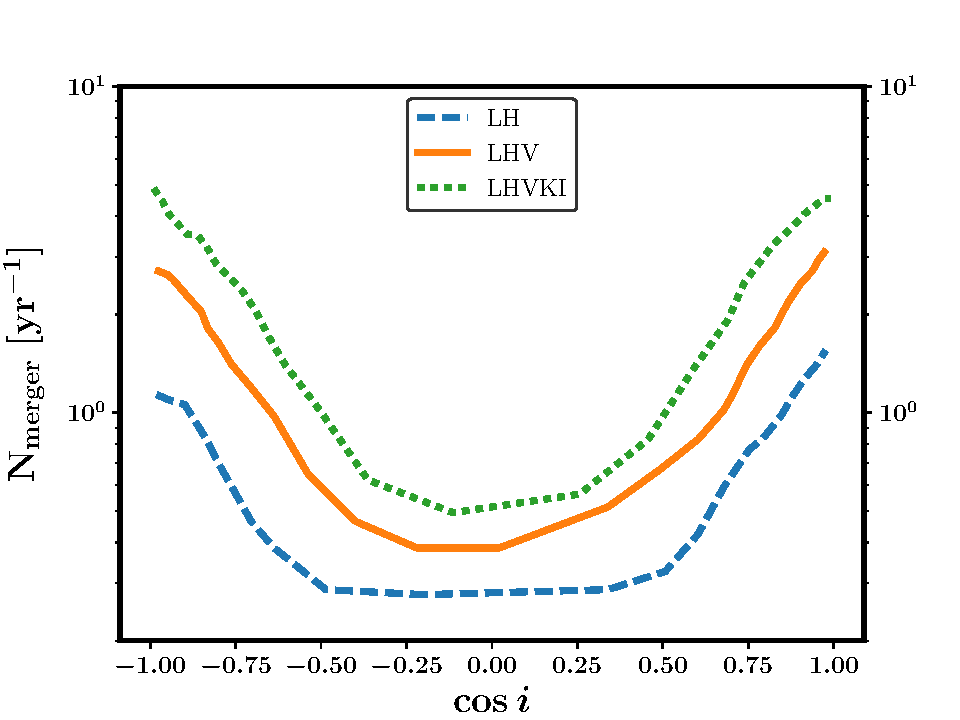
\includegraphics[scale=0.6]{BNSMr_lower_limits}
\caption[The lower limit of the binary neutron star merger rate for past, present, and future gravitational wave networks]{The lower limit of the binary neutron star merger rate [BNSM] as a function of the inclination of the normal to the merger plane with respect to the line of sight of the observer, $i$, for the Livingston-Hanford [LH] configuration in [blue] dashed line, the Livingston-Hanford-Virgo [LHV] configuration in [orange] solid line, and the future Livingston-Hanford-Virgo-KAGRA-India [LHVKI] configuration in [green] dotted line. Owing to the weak dependence of the deduced $ \Rcap(z) $ on $n$ [see Figure \ref{fig:Rdot_of_z--short}], the most likely scenario [from population synthesis studies] of $n = 1.0$ has been shown. The data for the limiting distance of the GW networks used for this purpose have been taken from \citealt{Saleem_et_al.-2018-MNRAS}.}
\label{fig:merger-rate}
\end{center}
\end{figure}






\section{Conclusions}
\label{sec:conclusions--SGRBs}
In this work, I have combined the accurate spectral energy and redshift measurements of $15$ SGRBS available till date, and found a significant linear correlation between the spectral energy peak in the source frame with the source luminosity, also known as the `Yonetoku correlation'. Next I have used this correlation to derive `pseudo-redshifts' of all SGRBs with measured flux, including \B, \s, and \f\ GRBs. Although the redshift distributions of the sample of $30$ SGRBs with known redshifts are not reproduced for the full redshift range, it is found that $25$ of these GRBs are located at $z < 1.0$, against the expectations from population synthesis studies. Furthermore, the pseudo-redshifts of all instruments agree well with the observed redshift distribution when limited to this redshift range. Thus, instrumental selection effects are understood to play a role in the non-detection of higher-redshift SGRBs. This provided confidence to use the pseudo-redshifts of the full catalogues to calculate their luminosities. This method does not claim to accurately predict the redshifts of individual bursts, but successfully mitigates the problems of having a statistically limited as well as selectively biased sample of bursts for the study of the luminosity function.

Assuming standard delay between the cosmic star formation and the binary neutron star mergers, which are thought to the progenitors of SGRBs, I attempted to fit the observed luminosity distribution of the largest SGRB sample of $757$ bursts studied till date. The simple powerlaw model of the LF is ruled out with high confidence. Both the exponential cutoff powerlaw [ECPL] and the broken powerlaw [BPL] model are found to fit the data of all three GRB-detectors, with the additional complication that the detection probability is different for \B\ compared to \f\ and \s. It is not possible from the current dataset to compare between the quality of fits between these two models, however. The low-luminosity index of the BPL model [$\nu_1$] is found to be weakly constrained below, although the constraints on the higher luminosity index $\nu_2 \sim 1.85$ and the break luminosity $\Lb \sim 1.50$ are much tighter. For the ECPL model, the powerlaw index $\nu \sim 0.7$ is well-constrained, and although the break luminosity is weakly constrained above, it is at least a few times higher than for the BPL model. Unlike in the case of long GRBs, it is not necessary to invoke any redshift dependence of the break luminosity, consistent with existing works in the SGRB literature. The current work is purely empirical in nature, and does not attempt to provide physical explanation of the LF models, which should be independently pursued via detailed phenomenological models of SGRBs.

The bestfit models are then used to make predictions of the SGRB detection rate of \AS -CZTI, implying that at least $\sim 20$ GRBs are undiscovered till date in the CZTI data by subjective triggered searches. They are also used to estimate the future prospects of the \D\ mission, and the prospects look really bright. The models are also used to derive the observed event rate of SGRBs, which is found to be weakly dependent on the assumed delay distribution. Adopting conservative limits of the jet opening angle, this is converted to get the true event rate of SGRBs. Assuming that each SGRB is produced from a binary neutron star merger [BNSM], this rate is then used to calculate the rate of BNSMs detectable by the past, current and upcoming global GW detector networks. Robust lower limits of $1.87 \, \py$ for the LHV and $3.11 \, \py$ for the LHVKI networks are derived, while the true rates may be significantly higher. The uncertainty on the rate of BNSMs calculated via the only confirmed BNSM detection via gravitational waves presented in the discovery paper of GW170817 \citep{GW170817-2017}, as well as the uncertainty on the SGRB rate derived from this work, are large. This makes it impossible to rule out the scenario that not all mergers produce SGRBs. The presence of a tension between these independently derived rates can have significant implications on the physics of the merger ejecta. Similar extensive electromagnetic follow-up campaigns of the future BNSMs detected via gravitational waves will be able to make more conclusive statements about the physics of the merger ejecta on a case-by-case basis.


\chapter{Noise analysis of CZTI data}
\label{chap:noise}
\begin{checkit}
This work will be reported in \emph{Paul et al., 2019, Experimental Astronomy}. I would like to sincerely thank Professor A R Rao, my PhD advisor, for giving me the opportunity for doing this work, and the permission to use the L2 CZTI data for a number of sources as and when required; Professor Dipankar Bhattacharya in IUCAA [Pune, India] for encouragement and support throughout the course of the work; Mithun NPS in PRL [Ahmedabad, India] for his extremely helpful suggestions at crucial stages of the work, as well as long discussions clarifying doubts regarding the existing pipeline and its data files. Last but not the least, all the data used in the work were kindly made available by the CZTI-POC [Payload Operation Centre] in IUCAA [Pune, India], all queries regarding which were timely attended by the people there, to whom collectively I extend sincere thanks.
\end{checkit}



\section{Introduction}
\label{sec:introduction--noise}
In Chapters \ref{chap:LGRBs} and \ref{chap:SGRBs}, it was shown that \AS -CZTI misses out on a number of GRBs, both long [Section \ref{subsec:predictions_for_CZTI--long}] and short [Section \ref{subsec:predictions_for_CZTI--short}]. The reasons are investigated in this chapter via a thorough re-look at the data analysis pipeline in place for CZTI.

In the CZTI terminology, an `event' is a trigger of any of the pixels, associated with an unique time-stamp, the pixel co-ordinates, and the `pulse height amplitude' or PHA, which is linearly related to the energy of the photons that triggered the pixel. Being a wide-field open detector, CZTI detects photons from all directions within its wide FOV. These photons include those from the target source, called `science' events, as well as those induced by other sources. The latter can include a steady rate of events induced by the charged particle environment of the detector, which other than showing predictable variation with the satellite co-ordinates, should show uniform random distribution about the mean. These events are called `background' events. On top  of this, events may be generated by the peculiarities in the detector and may not be triggered by photons in the first place. These need to be identified and removed before doing any scientific investigation of the events from the target source both in the temporal and energy domains, and are called `noise' events. Only a careful analysis of the data can precisely define characteristics of noise, and subsequently eliminate them for the study of the science data.

The presence of cosmic ray induced noise events was deduced during the first days of the mission, and a simple algorithm implemented in the existing CZTI pipeline to eliminate them from the science data. They are easily distinguished from science events due to the temporal characteristics: they all `bunch' together within the smallest interval of time resolvable by the CZT pixels, $20 \, \mus$ \citep{Bhalerao_et_al.-2017-JApA}. A steady stream of these `bunches' triggered by cosmic rays continuously bombard the detector plane. They temporally track the variation of the cosmic rays bombarding the entire satellite, independently measured by the Charged Particle Monitor [CPM] on-board \AS\ \citep{Rao_et_al.-2017-JApA}.

In this work, we have conducted a careful analysis of the data collected by CZTI for a number of GRBs. It is shown via careful reasoning that improvements in our understanding of bunches can be made. `Double-events' are those that occur on neighbouring pixels at the same time [i.e. within $20 \, \mus$], and are used for polarization measurements by CZTI \citep{Chattopadhyay_et_al.-2014-ExA, Chattopadhyay_et_al.-2017-arXiv}. The effect of electronic noise on double-events is quantified by studying the behaviour of the bunched events during GRBs. Moreover, identification of heavy deposition of charge by very high energetic particles is done via patterns on the detector modules that are characteristic of pixelated detectors collecting data at such high time resolutions. A new algorithm is developed which automatically identifies and removes these events from the data to create further cleaned science data.

The software has been tested in the \textsc{python} programming language. The scripts have being made publicly available at: \url{https://github.com/DebduttaPaul/useful_functions_for_CZTI_data_analysis}. The effects of of cosmic rays via bunches are carefully reinvestigated in Section \ref{sec:Bunchclean}, suggesting improvements of the current data flow in the existing CZTI pipeline. The effect of these `bunched' events on genuine events are quantified. In Section \ref{sec:Gross_noisy_pixels}, the flagging of grossly noisy elements are re-examined. In Section \ref{sec:DPHclean}, the effect of higher energetic cosmic rays on the CZTI data are reported, via an algorithm detailed in Appendix \ref{appendix:DPHstructures}. In Section \ref{sec:conclusions--noise}, concluding remarks are presented.


\section{Re-look at `cztbunchclean'}
\label{sec:Bunchclean}
The overall instrument configuration, the detectors and electronics, the data characteristics, processing pipeline and default products have been discussed in detail in \cite{Bhalerao_et_al.-2017-JApA}. All the work carried out in this chapter uses the astronomer-friendly `Level 2' [L2] FITS files created by the Payload Operation Centre [POC] of CZTI, located in the Inter-University Centre for Astronomy \& Astrophysics [IUCAA] in Pune, India. This is executed by the first task in the CZT pipeline\footnote{\url{http://astrosat-ssc.iucaa.in/uploads/czti/CZTI_level2_software_userguide_V2.1.pdf}}: the  \textbf{cztscience2event}. The on-board bunchclean identifies the bunches present in the data, and removes the events except three events at the boundaries of each bunch for the purpose of latter identification; more details can be found in the above document. The next task in the pipeline is \textbf{cztbunchclean}, which removes the bunched events in the data remnant after the onboard bunchclean. In addition, currently it removes data for certain lengths of time \emph{skipT1}, \emph{skipT2}, \emph{skipT3} after the bunches, depending on the number of events in the bunch, termed as \emph{bunch\_length\_threshold}. The values for these parameters have been set somewhat arbitrarily. In this section, we take a re-look at this task, and suggest alternatives to the parameters in the existing pipeline. For this, we have additionally used the data in the bunch files created by \textbf{cztscience2event}, to be henceforth termed as `bunch-files'.

\subsection{Redefining bunches}
\label{subsec:redefining_bunches}
The understanding behind the idea of bunches is that each bunch is created by one cosmic ray particle generating a series of electronic events within timescales shorter than the instrumental resolution of $20 \, \mus$. If such is the case, then respective bunches are independent of each other, and the interval between one bunch and the next, $\Delta T$, is expected to follow a smooth distribution. On plotting the histogram of $\Delta T$ by using the bunch data, it is clearly seen that such is not the case, see \eL\ of Figure \ref{fig:bunch_redefinition}. This leads one to assume that the electronic effects of a single charged particle lasts for more than the time-resolution of the instrument. Hence we propose to redefine bunches such that, if the interval between one bunch and the next is less than a certain threshold $t_2$, then these two bunches are understood to be created by the same cosmic ray particle and all the data within it are clubbed to a single bunch, henceforth termed a `super-bunch'. Empirically, it is seen that the sharp spike is removed on choosing $t_2 = 60 \, \mus$. For $t_2 = 40 \, \mus$, the spike is still clearly visible, whereas for $t_2 = 80 \mus$, the spike is replaced by a dip, clearly showing that it is an overkill. Thus, $60 \, \mus$ is optimal, see \eR\ of Figure \ref{fig:bunch_redefinition}. It is observed that less than $10 \%$ bunches are redefined as `super-bunches'.

\begin{figure}
\begin{center}
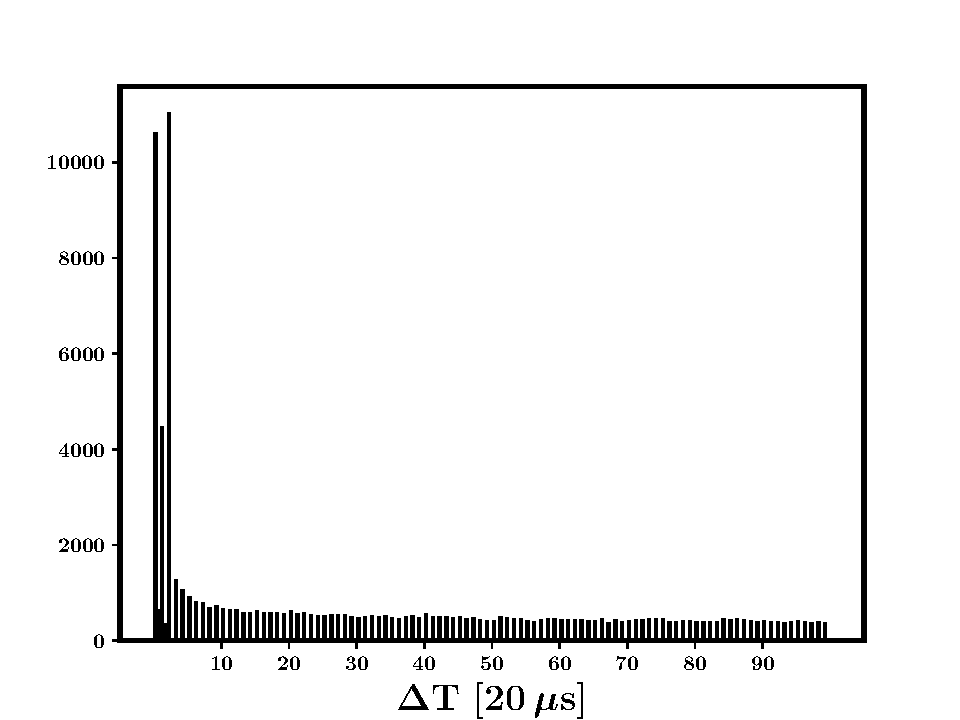
\includegraphics[scale=0.42]{GRB160802A--Q3--Interval_between_Bunches_Histogram--raw_data}
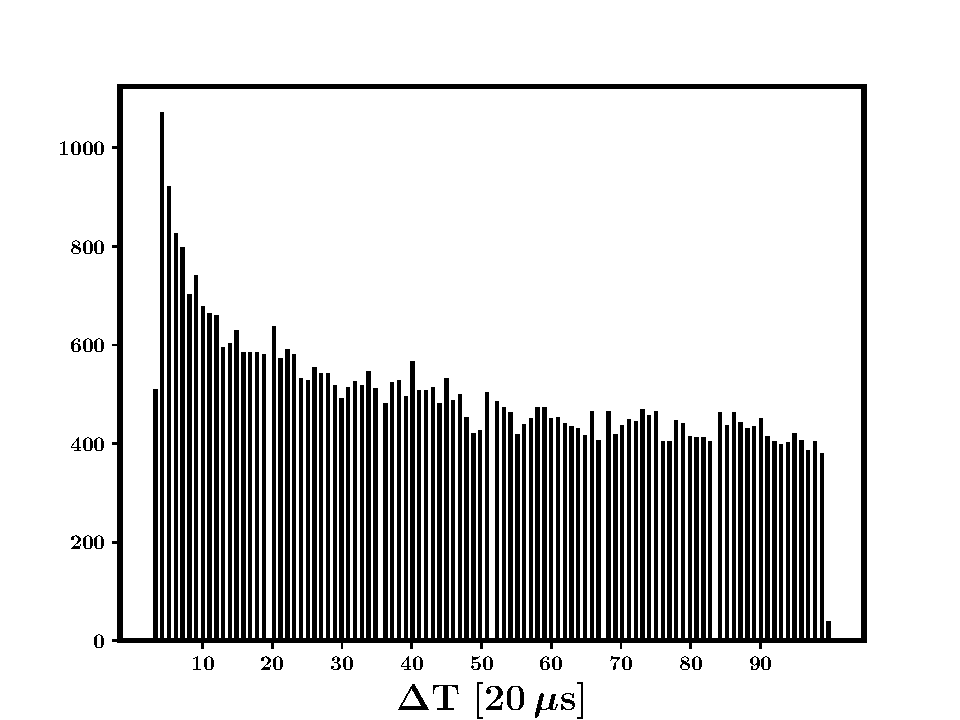
\includegraphics[scale=0.42]{GRB160802A--Q3--Interval_between_Bunches_Histogram--after_bunch_redefinition}
\caption[The re-definition of bunches]{$\Delta T$ is defined as the time interval between the end of a bunch and the start of the next bunch. \eL: Bunch data after \textbf{cztscience2event}. The histogram peaks at small $\Delta T$ clearly showing that the definition of bunches is incorrect. The parameter for bunch redefinition, such that the histogram becomes smooth is referred to as $t_2$. \eR: With $t_2 = 60 \, \mus$, the histogram indeed becomes smooth. Although the above plots are taken from one orbit of March background data, this observation is true for all datasets examined. The first point in corresponds to the bunch redefinition timescale, and is an artefact created due to the limitation of the way division is carried out in the binary system; it persists whatever value of $t_2$ is used, but is unimportant for our purposes.}
\label{fig:bunch_redefinition}
\end{center}
\end{figure}

\subsection{Post-bunch cleaning}
\label{subsec:post-bunch_clean}

\begin{figure}
\begin{center}
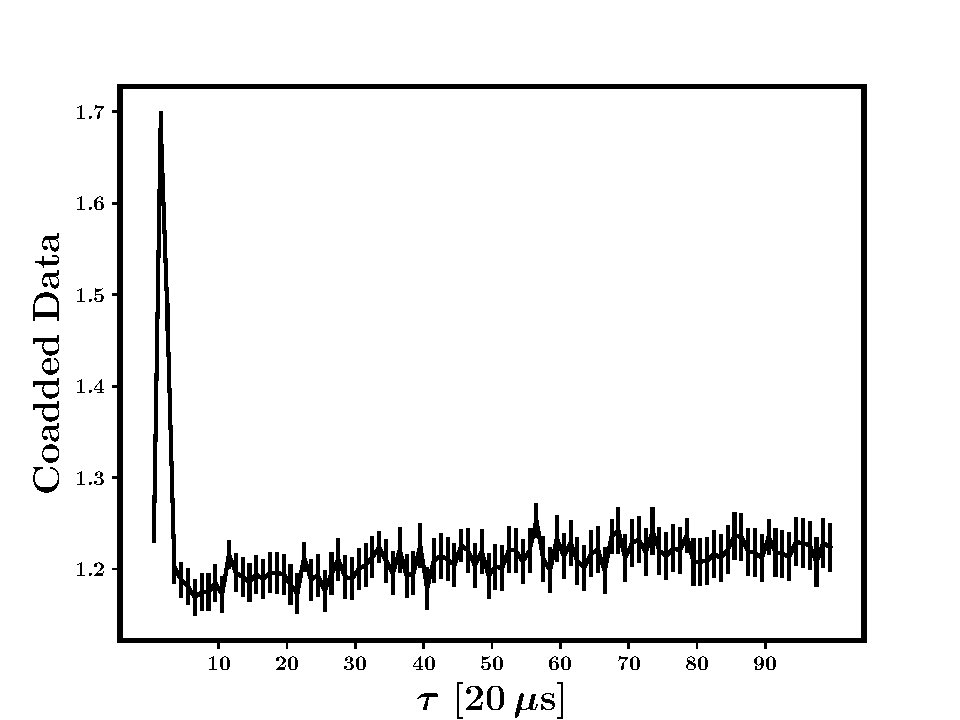
\includegraphics[scale=0.42]{GRB160802A--Q1--LC--raw_data}
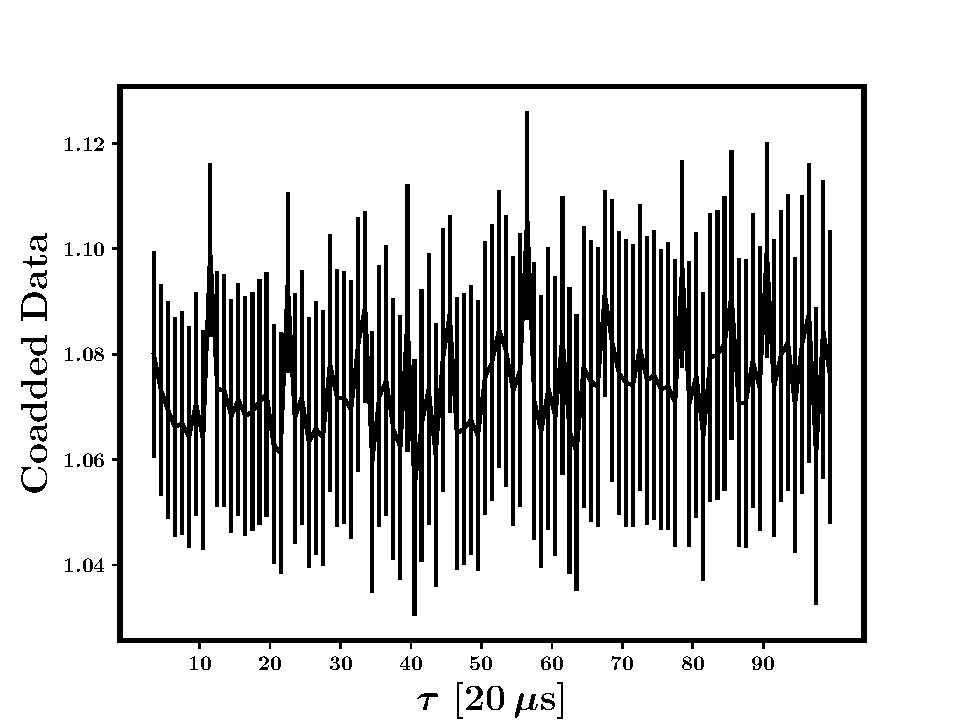
\includegraphics[scale=0.42]{GRB160802A--Q1--LC--after_new_bunchclean}
\caption[The remnant effect of \textbf{cztbunchclean}]{\eL: A sharp drop is seen at timescales lesser than $60 \, \mus$ if co-added lightcurve, corrected for the exposure, is made from data post bunches, even after redefining bunches. This implies that post bunches, significant amount of electronic noise, created by the bunches, is persistent. Hence, data post bunches is removed up to the parameter $t_3$. \eR: After flagging \emph{all} data post bunches, with $t_3 = 60 \, \mus$, the co-added lightcurve looks flat as expected, all the way up to $2$ ms, validating the assumption. All errors assume that the data is Poissonian, which is strictly true for the part away from the spike in \eL.}
\label{fig:postbunch_flagging}
\end{center}
\end{figure}


As noticed earlier, the electronic effects of cosmic-ray particles persist for some amount of time post-bunch, after initially triggering a series of events in the detector. We parametrize this timescale  as $t_3$, similar to \emph{skipT1}, \emph{skipT2}, \emph{skipT3}. To estimate the optimum value of $t_3$, we plot co-added lightcurves of events after the bunches. That is, we choose only the data from the end of each bunch to the next bunch, including the superbunches defined in Section \ref{subsec:redefining_bunches}, define the end of the bunches as $t = 0$, order the dataset thus formed from all the bunches, and then add these datasets. Shown in Figure \ref{fig:postbunch_flagging} is the ratio of this co-added data to the total exposure, where the exposure for each bunch is defined as the total number of instances that data is available between the chosen bunch and the next. This ratio is chosen to remove the overall Poissonian trend of the co-added data with time, and look for any remnant effects. If the data is fully Poissonian, then it should vary randomly about unity, for all times. In the \eL\ of the Figure, we see a sharp rise and fall at the smallest of $t$, which is indicative of remnant electronic effects even after redefining the bunches as described in Section \ref{subsec:redefining_bunches}.

We experiment with different values of $t_3$. On choosing  $t_3 = 60 \, \mus$ and removing data for $t_3$ after each bunch [including superbunches], the co-added lightcurve indeed becomes flat around unity, implying that the removal of cosmic ray induced noise is finally complete. \eR\ of Figure \ref{fig:postbunch_flagging} demonstrates this.

We have re-examined whether flagging only the affected detector modules also give the same result. For this we used long stretches of the same data, and experimented with different values of \emph{bunch\_length\_threshold} to check whether heavier bunches affect nearby detector modules as well. It is found that that there is no difference to the resulting cleaned data if selective cleaning is done to only affected detector modules or not, based on \emph{bunch\_length\_threshold}. The optimized value of $t_3$ is so small that most of the data successive to the bunches are mostly in the same modules, hence no difference is made. Thus, instead of three parameters for post bunch cleaning, only one is sufficient. $t_2 \sim t_3$ leads one to assume that the physical mechanism behind both the effects are same, that is electronic noise in the hardware, which is quantified in the next subsection.

The newly proposed method of cleaning the L2 data of bunches, constituting the two steps demonstrated in Section \ref{subsec:redefining_bunches} and \ref{subsec:post-bunch_clean}, is to be henceforth collectively and simply called `bunchclean', as against `on-board bunchclean' which leaves three events from each bunch in the dataset, and the pipeline task \textbf{cztbunchclean} which invokes the usage of the parameters \emph{skipT1}, \emph{skipT2}, \emph{skipT3}, \emph{bunch\_length\_threshold}.


\subsection{Using bunches to quantify electronic noise created by source photons}
\label{subsec:electronic_effects}

We have carried out a preliminary examination of lightcurves of bunches for a few datasets, i.e. the time-series of the number of bunches detected, see Figure \ref{fig:bunch_enhancement_during_bright_GRBs} for an example. Sudden increase of the bunch-rate lasting for a few seconds are seen in such lightcurves, corresponding to possible increase of cosmic ray induced events. These features appear randomly in different datasets and quadrants. Moreover, they are almost always due to bunches with bunch-length [total number of events constituting a bunch] equal to $3$ instead of higher. Sometimes bunches of greater lengths show gradual increase from the continuum level, but these features are not as sharp; moreover, they appear uncorrelated to bunches of length $3$.

Temporal features in the bunches lasting for $\gtrsim 10$ s always appear at the same instances for bunches of different lengths. These are extremely rare [$\sim$ once in $10$ orbits of data] phenomenon, and seem to affect Q3 the most, followed by Q2; however this statement is subject to low-count statistics. If it is true on the other hand, it can be understood to be caused by the fact that these quadrants are in the open side of the satellite and is hence prone to high energetic charged particles: Q3 is open from two sides as compared to one for Q2, wheres Q0 and Q1 are closed by high-Z absorbers from all sides.

\begin{figure}
\begin{center}
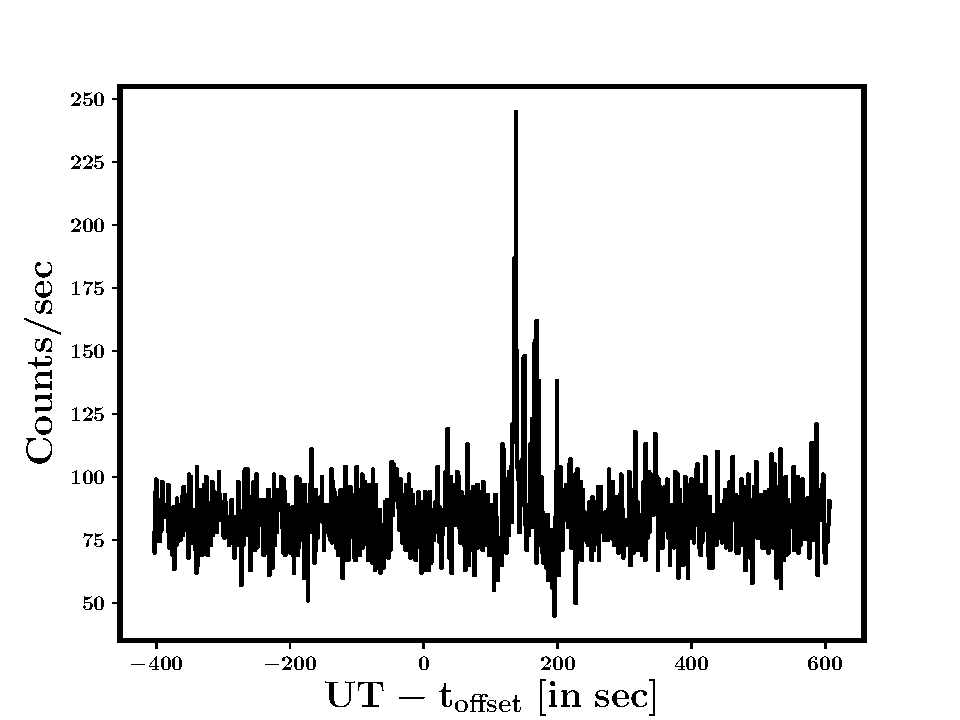
\includegraphics[scale=0.42]{GRB160821A--Q1--all_bunch_LC--1s}
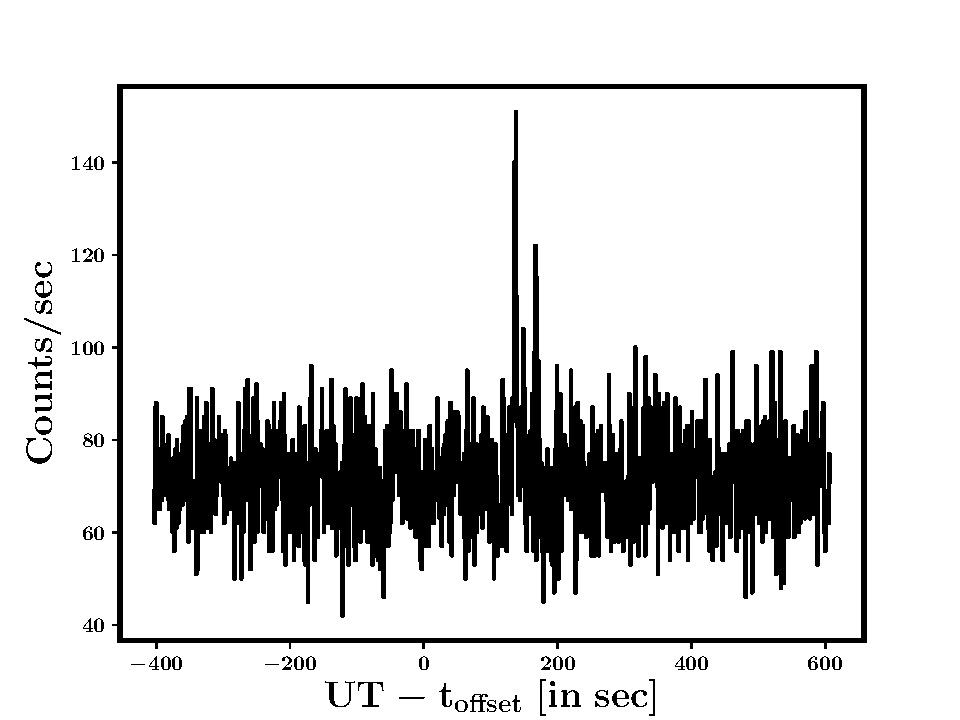
\includegraphics[scale=0.42]{GRB160821A--Q1--Tg_bunch_LC--1s}
\caption[Enhancement of number of bunches during bright GRBs]{Bunch lightcurves for bright GRB160821A, with the time axis offset to the known GRB trigger time [note that the trigger time in all quadrants of CZT data as well as Veto for this GRB is offset by $\sim 150$ s from the value reported by IceCube]. Such an enhancement is not expected if all bunches are due to cosmic rays. \eL: All bunches. \eR: Bunches with total number of events greater than $3$ also show enhancement. Increasing this threshold does not suppress this effect, implying that GRB photons trigger electronic events mimicking as short as well as bunches.}
\label{fig:bunch_enhancement_during_bright_GRBs}
\end{center}
\end{figure}


If bunches are all indeed created by cosmic ray photons, then they should not show any enhancement during GRBs. Figure \ref{fig:bunch_enhancement_during_bright_GRBs} demonstrates that bunches do exhibit such an unexpected enhancement, although this phenomenon is extremely rare, seen for only the brightest of GRBs, e.g. GRB160623A, GRB160802A, GRB160821A. During these bright flashes, the chance-coincidence of single events with others may mimic double-events, and similarly, their chance-coincidence with double-events may mimic bunches. Let us denote the average single-event rate as $r_{\rm{1,b}} \sim 200 \, \ps$, the average double-event rate as $r_{\rm{2,b}} \sim 70 \, \ps$ etc., the temporal resolution of CZTI as $\delta t =  20 \, \mus$, and the excess single-event rate during a bright GRB as $r_1 \sim 2000 \, \ps$. Then the chance-coincidence production rate of double-events during a GRB is $r_{\rm{1}} r_{\rm{1,b}} \delta t = 8 \, \ps$, and the chance-coincidence production rate of bunches is $r_{\rm{1}} r_{\rm{2,b}} \delta t = 2.8 \, \ps$. The chance-production rate of higher length bunches will be even smaller, and hence can be neglected. Thus, we see that only chance-coincidence cannot explain the enhancement of bunches during bright GRBs, falling short by at least one order of magnitude. Hence the identification of all bunches with cosmic rays is questionable. Moreover, the enhancement correlates with the GRB flux, being $\sim 80 \, \ps$ for GRB160623A, GRB160802A and $\sim 150 \, \ps$ for GRB160821A, the latter being brighter than the former two by roughly the same factor. We attempted to segregate this effect into bunches of different lengths, i.e. examined that whether the enhancement of the bunch-rate is only for bunches lesser than a certain length. Although the enhancement during the GRBs is progressively lesser for bunches of higher lengths, for GRB160821A the enhancement is clearly seen for bunch lengths at least up to $6$ [see \eR\ of Figure \ref{fig:bunch_enhancement_during_bright_GRBs}].

\begin{figure}
\begin{center}
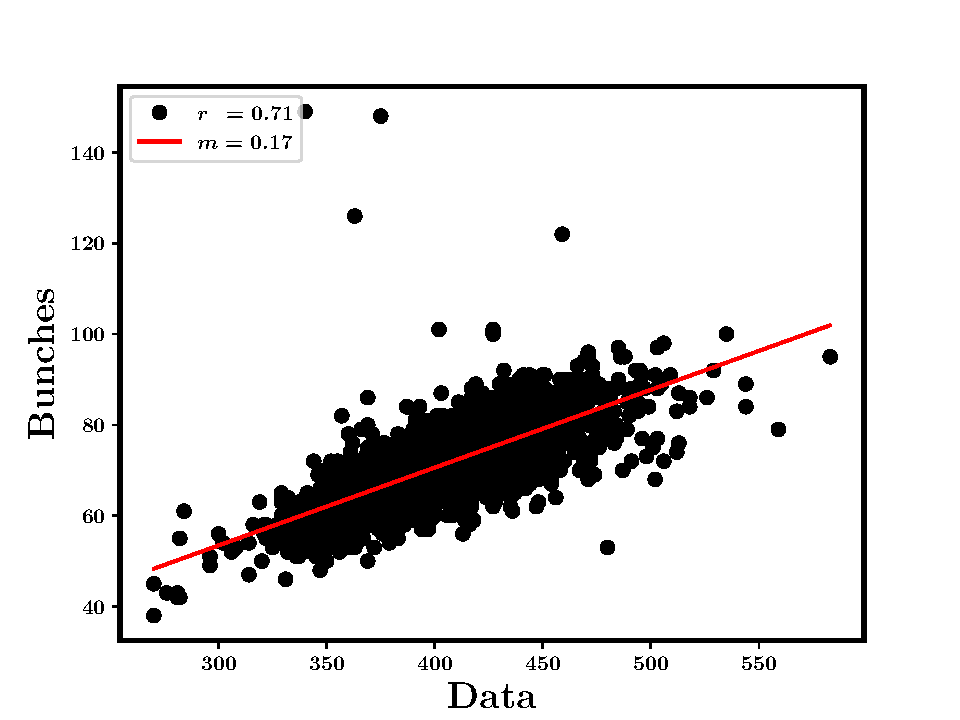
\includegraphics[scale=0.42]{GRB160821A--BKG_fit}
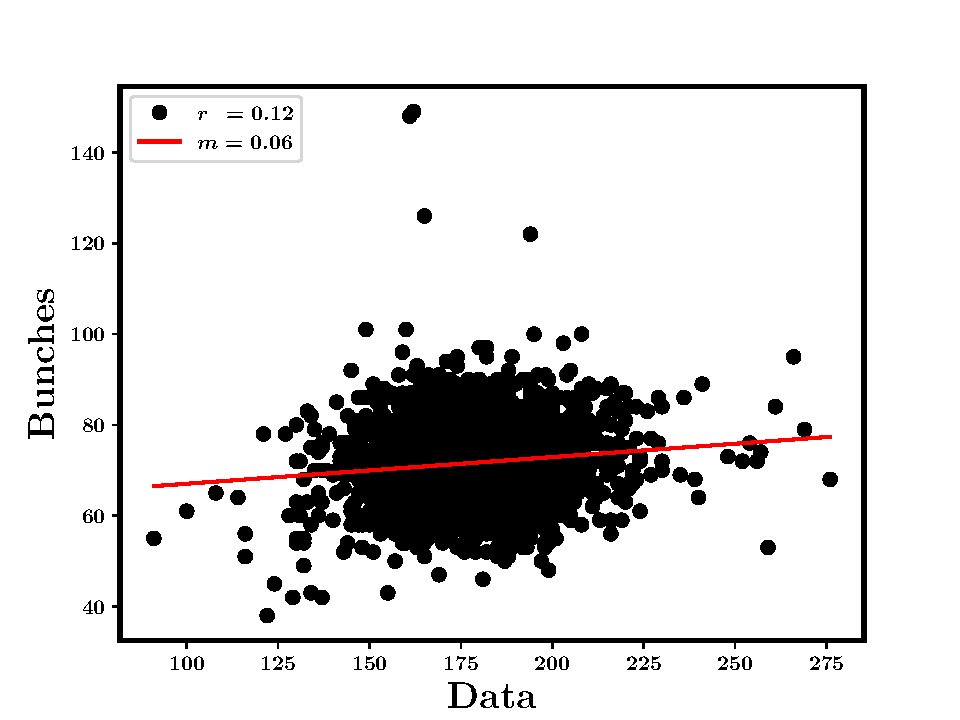
\includegraphics[scale=0.42]{GRB160821A--BKG_fit--with_Bunchclean}
\end{center}
\begin{center}
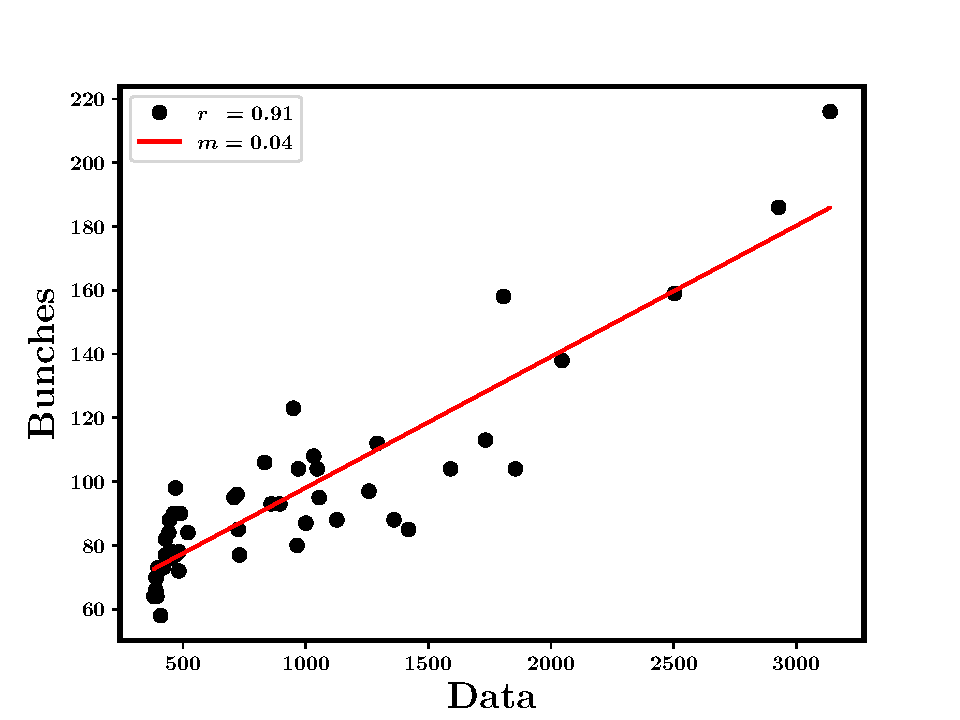
\includegraphics[scale=0.4]{GRB160802A--GRB_fit}
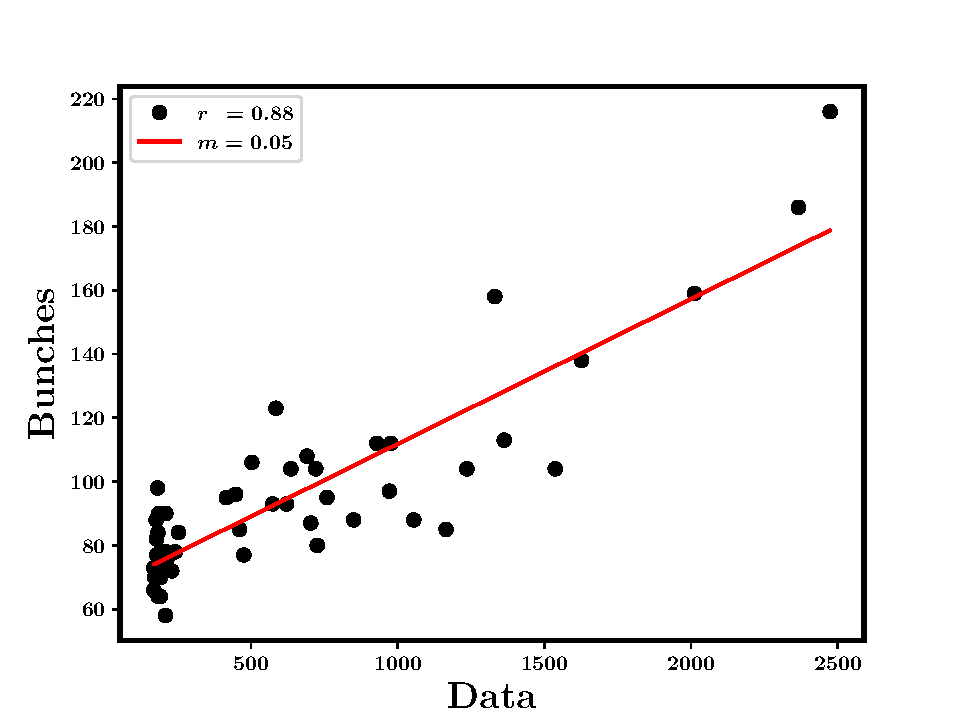
\includegraphics[scale=0.4]{GRB160802A--GRB_fit--with_Bunchclean}
\caption[Correlation between bunch-rate and event-rate]{\emph{Top}: Bunch-rate versus event-rate [corrected for livetime] away from the duration of the very bright GRB160821A. $r$ is the Pearson correlation coefficient, $m$ is the slope of the fitted straight line. \eL: In the raw data including bunches, i.e. before bunchclean. \eR: After bunchclean: the correlation is gone, and the scale in the x-axis is reduced by half. The slope is reduced by a factor of $\sim 3$. \emph{Bottom}: During the duration of the bright GRB160802A. \eL: Before bunchclean. \eR: After bunchclean; the correlation is still present. It is primarily driven by the small number of bins corresponding to the GRB excess. The slope obtained is comparable for all the three bright GRBs examined, before as well as after bunchclean. This clearly proves that there is a driving mechanism of the bunch excess by the GRB excess, independent of datasets used or the duration or flux of the GRBs. The similarity in the slope with that of the data devoid of GRBs post cleaning [\emph{Top-Right}] is also indicative of the universality of this driving mechanism, implying that \emph{all} source photons, including sky background, create such an electronic effect. Not all bunches can hence be thought to cosmic ray triggered. However, this gives an overall scaling in the number of bunches as well as double events. All bunches, whether induced by cosmic rays or this electronic mechanism, need to be removed anyway.}
\label{fig:correlations}
\end{center}
\end{figure}


The bright GRBs provide the opportunity to study electronic effects that remain otherwise hidden in the data. For these GRBs, we create time-series of the total data, as well as the number of bunches, binned at the same timescale. Then we plot these two time-series data against each other, shown in Figure \ref{fig:correlations}. First we consider time intervals that do not include the GRBs. A clear correlation is seen between the two time series. However, the correlation vanishes on executing `bunchclean'. The correlation, and its absence on implementing bunchclean on the dataset, is simply due to the fact that the overall event-rate depends on the cosmic ray induced events. This becomes clear by considering the fraction of the total events in the L2 data that happen to be bunches.

From the on-board bunch data available in the bunch files, we compute that the average bunch-length is $6$. We note that, although it varies with datasets and orbits, the average bunch-rate is $70$. Hence, the average event-rate in the raw data [i.e. before on-board bunchclean] due to the bunches remaining in the L2 data is $\sim 400$. We also note that the event-rate in the data after on-board bunchclean is also of the same order [$\sim 400$], and this is consistent with the known fact that the total event-rate before on-board bunch-cleaning is roughly twice the average number of events before bunchclean. This can be further illustrated from the slope of the best-fit straight line, which comes out to be $\sim 0.16$:

\begin{eqnarray*}
{\rm slope} \, (0.16) = \dfrac{{\rm avg\, bunch\, rate}}{{\rm avg\, data\, rate}} \implies {\rm avg\, bunch\, rate} = 0.16 \times {\rm avg\, data\, rate}.
\end{eqnarray*}

\begin{eqnarray*}
\therefore {\rm avg\, event\, rate\, due\, to\, bunches} & = & {\rm avg\, bunch\, length \,} \times {\, \rm avg\, bunch\, rate} \\
 & = & 6 \times ( 0.16 \times {\rm avg\, data\, rate}) \\
 & = & {\rm avg\, data\, rate}.
\end{eqnarray*}

Next, we plot the two time-series by considering data only around a GRB, as shown in Figure \ref{fig:correlations}, \emph{Bottom}. Again a clear correlation is seen, irrespective of whether bunches are removed or not. However, the slope is reduced by a factor of $\sim 3$ as compared to the slope from the correlation seen earlier [i.e. for data not including the GRB time]. Moreover, this slope is consistent between all the three GRBs for which bunch-excess is seen. The excess of event-rate from the background rate is less than $500$ counts $\ps$ for weaker GRBs. $500$ falls at the lower end of the correlations, explaining why significant bunch excesses are not seen during weaker GRBs. It implies that the inherent cause of these excesses are similar for all GRBs, and the effect is linear in the rate of incident photons. The slope can be used to calculate the probability of bunches being created from genuine photons, if it is assumed that \emph{all} incident photons, whether they are from GRBs, background or created by cosmic rays, create additional electronic effects that mimic bunches. This assumption is in fact corroborated by the fact the slope obtained from the fit during the GRBs is of the same order as that obtained from the fit from the data away from the GRBs post bunchclean, as illustrated in Figure \ref{fig:correlations}, \emph{Top-Right}. This conclusion is also seen to be independent of the dataset used, pointing to an universality of the driving mechanism.

Since the slope is $\sim 0.05$, the average number of bunches created by genuine photons is $0.05 \times 400 = 20$. That is, on an average, $20$ out of $70$ bunches are \emph{not} induced by cosmic rays. However, the impossibility of distinguishing cosmic-ray induced bunches with bunches created by photons, as well as the identification of the source photons from the artificial electronic events within the latter kind, means that it is always safe to remove bunches irrespective of the causal mechanism. The purpose of cleaning the data is to remove all events that are known to be created by anything other than source [including sky background] photons.

Assuming that the number of events in the electronically-generated bunches is $4$ \footnote{Although excess in the counts of different bunch-lengths are seen during GRBs, the excess becomes less prominent for bunch-lengths very much greater than $3$, resulting in the average number of events in the bunch-excess to have bunch-length of $4$.} , the number of such events flagged during bunchclean $\sim 20 \times 4 = 80$. After all processes of cleaning, we are left with a total number of $\sim 200$ events [both single and double events], which means out $\sim 400$ events that are flagged during on-board bunchclean + bunchclean, $\sim 20 \%$ are events due to \emph{source photon $+$ associated electronic noise} while the rest are events from genuine cosmic rays. If we extrapolate this idea to double events, we can say that $20 \%$ of the remaining double events are generated by electronics, and since these are also likely to be in adjacent pixels, they can mimic what we think are Compton-scattered double-events. This fraction is significantly higher than that can be produced by chance-coincidence of single events during extremely bright GRBs as calculated earlier, and can affect polarization measurements of these bright GRBs.


\section{Re-look at flagging gross noisy pixels}
\label{sec:Gross_noisy_pixels}

In the previous section, we have extensively discussed the task \textbf{cztbunchclean} of the CZT pipeline, and suggested an alternative task, simply referred to as the `bunchclean', consisting of two successive steps. In this section, we discuss the task \textbf{cztpixclean} in the current pipeline, which is the next successive step in the pipeline that takes up the removal of the noise events from the data. This task consists of two logical steps: the identification of extremely hot pixels and removal of all data from them, and the identification of pixels which are temporarily giving unexpected results.

Currently, the way to identify the grossly misbehaving pixels is to iteratively identify and flag those which show greater than $5 \sigma$ deviation in the total detector plane histogram [DPH], i.e. the histogram of the counts in the CZT plane, from the entire observation. Two modifications are attempted: one is to correct for the effective areas of the pixels [from \textbf{CALDB} file available along with the pipeline]; the other is to make the DPHs every $t_{{\rm avg}}$ during the observation, and scaling each DPH with its total counts before looking for outliers in the added DPH. The latter takes care of the variation of the event-rate within the particular observation, i.e. the variation of the background counts with the satellite position. Both the modifications are attempted individually as well as together, in the latter case in both possible orders. It is seen that the effective area of `spectroscopically bad pixels' generally get over-corrected if \textbf{CALDB} data is used, and this leads to the identification of these pixels as gross noisy pixels. Flagging spectroscopically bad pixels from the data itself, however, does not lead to any change in the converged solutions, whether the lightcurve weighting is done or not. This holds true up to $t_{avg} = 2$ s, below which statistical uncertainties in the lightcurve actually leads to incomplete identification of the gross noisy pixels. We conclude that the solutions obtained by the current method is optimal and also the most efficient. This is true even if there are bright GRBs in the data, because GRBs illuminate the entire quadrant instead of selective parts. Henceforth, we parametrize this step with $\gc$, which is the deviation [in units of $\sigma$] that is used to identify gross noisy pixels. The optimized value of $5$ does a satisfactory job in the sense that the solutions always converge to the same gross noisy pixels, roughly $10$ per quadrant, and are independent of the duration of the observation used [unless it is too small].

It is noted from the lightcurves of gross noisy pixels thus identified exhibit random and sudden features which are entirely uncorrelated with bunches, GRBs, features in the lightcurve of the Veto data, or even to each other. Occasionally they create loss of data-acquirement in other pixels because the number of events in these singular pixels themselves can be greater than the total allowed by on-board electronics. This effect is known, is taken care of while writing the `good time interval' [GTI] columns in the L2 file created by the current data pipeline. The exposure correction of lightcurves, known as the `livetime correction', accounts for this data loss.







\section{DPHclean}
\label{sec:DPHclean}
The second part of the current task \textbf{cztpixclean} identifies temporarily `flickering' pixels somewhat arbitrarily, based on the lightcurves of each pixel, and removing data if the countrate for an individual pixel becomes greater than a certain value. This might result in the removal of data during bright GRBs, which is what is indeed seen in the case of the bright GRBs. Currently, the CZT POC processes the data for bright GRBs separately to prevent the removal of GRB events. A careful re-look at this step of the task is made in the next section, leading to the discovery of higher energy cosmic rays in the data.

In the lightcurves made from the data after bunchclean and removing gross noisy pixels, strong temporary features lasting upto a few hundred milliseconds are observed [see Figure \ref{fig:GRB_zoom}]. By making detector plane histograms [DPHs] of the events that create these features, it is seen that these events cluster in some parts of the detector plane rather selectively. The timescale for detecting such clustering is examined, parametrized by $\tl$. Initially, such clustering are observed to be present for $5 \sigma$ outliers in lightcurves binned at $100$ ms. The events that contribute to the clustering are spread over timescales less than $100$ ms, and only very rarely involve two consecutive bins of $100$ ms. The automatic identification of such clustering in the DPHs, henceforth called `DPHstructures', is implemented by an algorithm called `DPHclean' detailed in Appendix \ref{appendix:DPHstructures}. Since this algorithm is independent of the total number of events in the DPH, the only constraint on $\tl$ is that it should be more than the duration of such events. $100$ ms is optimized in this regard, catching such clustering as well as being an order of magnitude smaller than the $\T$ of short GRBs, thus making it safe to allow independent identification of short GRBs even after the implementation of DPHclean.


\begin{figure}
\begin{center}
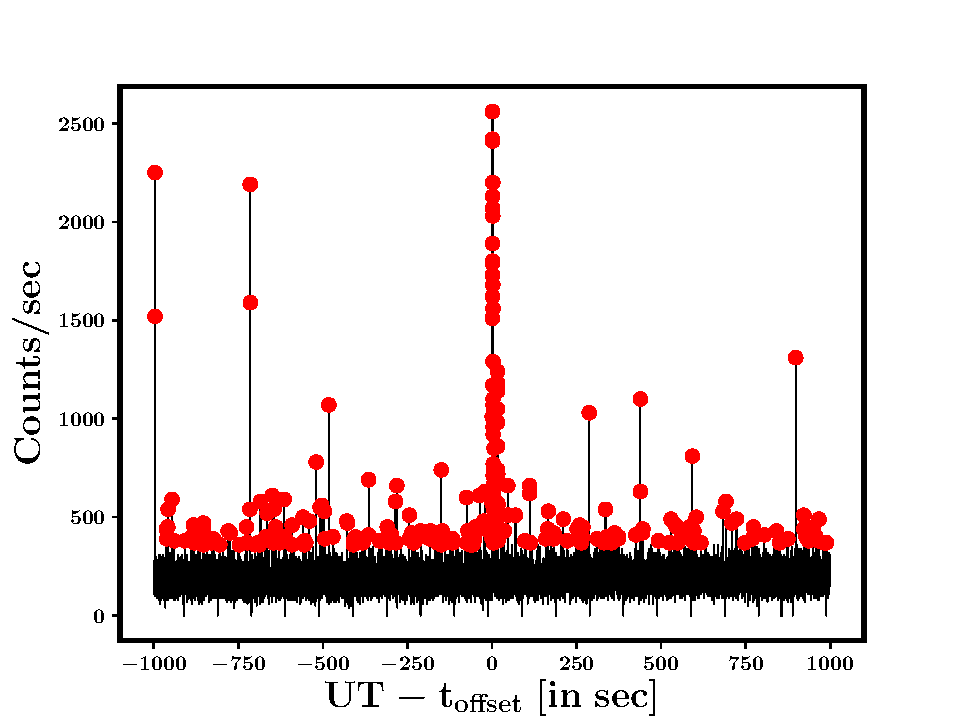
\includegraphics[scale=0.42]{GRB160802A--Q1--DPHclean_before}
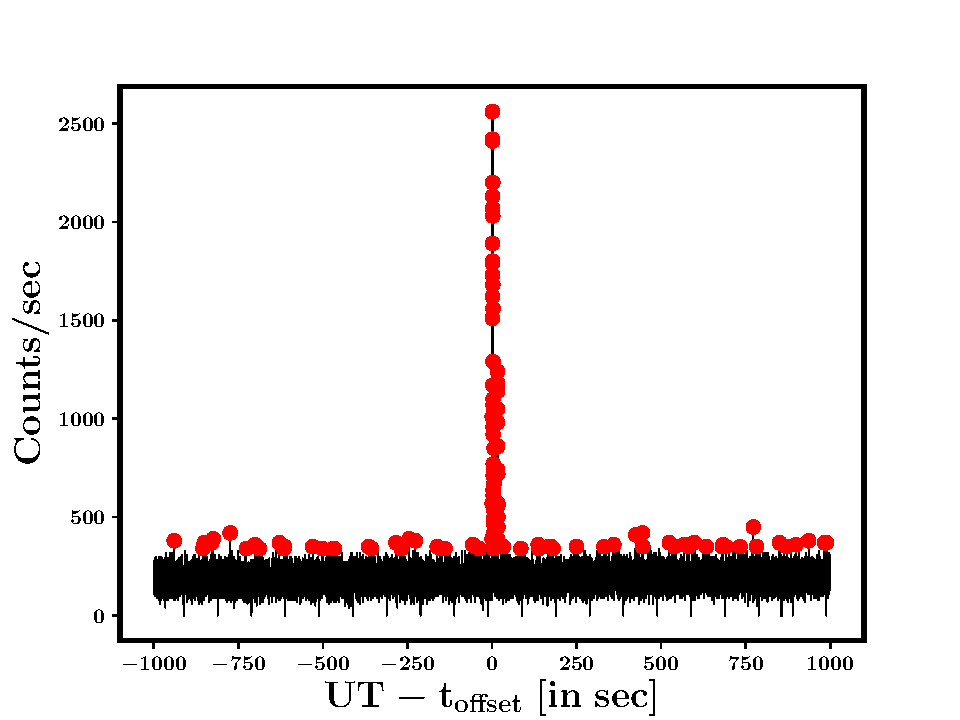
\includegraphics[scale=0.42]{GRB160802A--Q1--DPHclean_after}
\end{center}
\begin{center}
\includegraphics[scale=0.42]{GRB160802A--Q0--DPHclean_before--zoom}
\includegraphics[scale=0.42]{GRB160802A--Q0--DPHclean_after--zoom}
\caption[The effect of DPHclean on the lightcurves of GRBs]{Lightcurves binned at $\tl = 100$ ms before [\eL] and after [\eR] DPHclean near the bright GRB160802A, red points showing $2 \sigma$ outliers. \emph{Top}: longer stretch of Q1; \emph{Bottom}: zoomed for Q0 [hence scale is different]. It is noted that sudden features in the lightcurve are removed by DPHclean, but GRB photons are not flagged. The second feature within $20$ seconds of the start of the prompt emission is also a part of the GRB, and is seen distinctly in the zoomed lightcurves of all quadrants with a similar profile, so it is not be mistaken as noise.}
\label{fig:GRB_zoom}
\end{center}
\end{figure}


\begin{figure}
\begin{center}
\includegraphics[scale=0.5]{Histogram_of_Npoints--observed}
\caption[Histogram of the number of unique points in the DPHstructures]{Histogram of the number of unique points in the DPHstructures.}
\label{fig:histogram_of_observed_Npoints}
\end{center}
\end{figure}



A large fraction of the events clustered in DPHstructures occupy regions only a few pixels wide, see Figure \ref{fig:histogram_of_observed_Npoints}. Some of these DPHstructures includes pixels which register counts $4$ or higher in $100$ ms bins. Here it is pointed out that in case a DPH shows clustering, only those events in the DPH that are responsible for the same are removed from the data by DPHclean. It that has the ability to identify them, and in the presence of such clustered events even during bright GRBs, the algorithm selectively picks out only the events in the cluster and removes them, instead of the GRB photons. The advantage of such selective identification is evident. It is noticed that running this algorithm on \emph{all} DPHs made from a given set of data reduces the noise significantly more than selectively running it on [say $5 \sigma$] outliers in the lightcurve. To highlight the case that randomly distributed GRB photons are left unharmed by DPHclean, Figure \ref{fig:GRB_zoom} compares the lightcurve binned at $\tl = 100$ ms before and after implementing this step.
%For the purpose of the pipeline flow, however, it is safe to remove all DPHstructure events.


\begin{figure}
\begin{center}
\includegraphics[scale=0.42]{LC_of_bunches}
\includegraphics[scale=0.42]{LC_of_DPHstructures}
\caption[Lightcurves of bunches and DPHstructures for a full orbit data]{Lightcurves of bunches [\eL] and DPHstructures [\eR] binned at $ 100$ s, for a full orbit data. One of the quadrants [Q0] show a peak for the bunches, which is understood to be due to the rise of the number of bunches over several $1$ s intervals. However, such an increase is not seen for the same quadrant for the DPHstructures. The overall increase of the count-rate of both the bunches and the DPHstructures towards the end of the orbit as the satellite enters the SAA, indicates that both kind of events may be due to the common origin in charged particles.}
\label{fig:lightcurve_comparison_of_bunches_and_DPHstructures}
\end{center}
\end{figure}

\begin{figure}
\begin{center}
\includegraphics[scale=0.5]{delta_btn_DPHs_and_previous_bunch}
\caption[Histogram of the time difference between the start of a DPHstructure with the end of the bunch just preceding it]{Histogram of the time difference between the start of a DPHstructure with the end of the bunch just preceding it, denoted here as $\Delta T$. There is no non-statistical rise of the number of such coincidences all the way up to $\sim 100$ ms, indicating that there is no causal correlation between bunches and DPHstructures.}
\label{fig:correlation_between_bunches_and_DPHstructures}
\end{center}
\end{figure}


In  Figure \ref{fig:lightcurve_comparison_of_bunches_and_DPHstructures} are plotted the lightcurves of bunches and DPHstructures, both binned at $100$ s intervals for a full orbit data.  The overall rise towards the end of the orbit as the satellite enters the South Atlantic Anomaly [SAA] is clear for bunches, whereas for DPHstructures, it is only marginal. However, this similarity points to the origin of both kinds of events in charged particles. The quadrant-averaged orbit-averaged rate of DPHstructures is $0.245 \, \ps$.
%It is hypothesized that they are locally generated electronic noise or tails of cosmic ray bunches lingering in the data for timescales longer than bunches. On the other hand, it is most likely that the DPHstructures that cause strong outliers in lightcurves are caused by a physical mechanism that gives rise to genuine ionization in the detectors, and not random electronic noise.

We have investigated any possible temporal correlation of bunches with DPHstructures, to understand whether DPHstructures could be caused by heavy bunches. In Figure \ref{fig:correlation_between_bunches_and_DPHstructures} is shown the histogram of the difference between the start-time of a DPHstructure with the end-time of the bunch that just precedes it. No causality is found at time intervals less than $1$ ms. That is, bunches and individual DPHs are statistically independent events.
%This is concluded by rigorous investigation of the lightcurves of bunches and DPHstructures. The lightcurves of bunches with higher bunch-lengths are also considered for careful re-investigation, because being rarer than bunches of smaller lengths,  they may be due to higher energetic cosmic rays, thus falling in the continuum of the spectrum of the energy of the cosmic rays.


\cite{Segreto_et_al.-2003-A&A--INTEGRAL_cosmic_rays} [hereafter \citetalias{Segreto_et_al.-2003-A&A--INTEGRAL_cosmic_rays}] studied the detector characterisitics of the PICsIT detector plane on board INTEGRAL, and found events similar to DPHstructures. To investigate their cause, they plotted detector delay histograms [DDHs] corresponding to each DPHstructure. DDHs are histograms on the detector plane of the delay of the events contributing to a particular DPHstructure with respect to the first event. They found the evidence of two kinds of events: linear tracks, and a particular kind of delay pattern-- a gradual increase of the delay towards the centre of the ellipses that were illuminated. They explained these by the bombardment of the detector plane by charged particles or cosmic ray showers generated by hadronic and leptonic processes very close to the detector. They demonstrated that the delay in the first and last events in a particular DPHstructure being $\sim 100$ ms  could be explained by the saturation of the pixels by the extreme high energies of the charged particles, the pattern on the detector tracing the density of the cosmic ray showers in the logarithmic scale. Inspired by these findings, we plot DDHs for our DPHstructures, some examples are given in Figure \ref{fig:DDH}. We see two kinds of events:


\begin{enumerate}
\item Those tracing linear tracks indicating trajectories of physical entities along them [Figure \ref{fig:DDH}, \emph{Top}]. This points to the origin being charged particles which deposit their energy over multiple pixels that fall on its trajectory of motion through the detector.
\item Those with the delay being more in the inside of a cluster compared to its boundaries [Figure \ref{fig:DDH}, \emph{Bottom}].
\end{enumerate}

Both the kinds of events are in striking similarity with the DDHs observed in PICsIT on board INTEGRAL, and naturally leads one to the hypothesis that DPHstructures in CZTI are also created by the bombardment of high-energy charged particles or cosmic ray showers.

Some cosmic rays might deposit their energies over multiple pixels instead of a few because being more energetic than their counterparts that create bunches, they are above the detectable energy threshold of the pixels, thus saturating them. When the pixel output current drops below this threshold, they start registering events. The saturation timescale observed in the detectors then corresponds to the delay from the onset of the events created by these cosmic rays on the detector plane. The fact that DPHstructures are much less frequent than bunches, also corroborates such a hypothesis. Also, it naturally explains the delay pattern of the second kind, that is those with progressively higher delays towards the centre of the pattern \citepalias{Segreto_et_al.-2003-A&A--INTEGRAL_cosmic_rays}. When a cosmic ray shower hits the detector, the density of the particles in the shower are traced by the delay in the DDH. The delay timescale in the detector pixels are thus deduced to be a few $100$ milliseconds.


\begin{figure}
\begin{center}
\includegraphics[scale=0.42]{Q1--merged_35+36}
\includegraphics[scale=0.42]{Q1--merged_11114+11115}
\end{center}
\begin{center}
\includegraphics[scale=0.42]{Q1--merged_2853+2854}
\includegraphics[scale=0.42]{Q3--merged_7861+7862}
\caption[Detector Delay Histograms showing patterns similar to INTEGRAL-PICsIT]{Detector Delay Histograms: Plotted in colour are the delay of the particular event from the first event in the cluster, in milliseconds, as a function of the position in the detector plane. These examples last unusually long, covering two consecutive bins. In \emph{Top}, we observe linear tracks, the delay increasing along the track in \emph{Top-Right}. The delay patterns in \emph{Bottom} are remarkably similar to those seen in PICsIT on INTEGRAL due to phosphorescence-decays from events triggered by cosmic ray showers.}
\label{fig:DDH}
\end{center}
\end{figure}


The energy of the cosmic rays cannot be calculated directly. However, we place constraints on the energy of both bunches and DPHstructures from the observed rate of the events, assuming a standard spectrum of cosmic rays \citepalias{Longair-3rd_Ed.}:

\begin{equation}
\frac{\dd N}{\dd E} =  1.8 \times 10^4 \rm{\dfrac{nucleons}{s \, m^2 \, sr \, GeV}} \left( \frac{E}{1 \, \rm{GeV}} \right)^{-2.7}.
\label{eq:cosmic_ray_spectrum}
\end{equation}

We assume that the DPHstructures illuminate $10$ pixels on an average, which is an area of $160 \, \rm{cm^2}$, and integrate over all solid angles, between energy limits $E_{\rm{min}}$ and $E_{\rm{max}}$ and match them with the observed rates of bunches and DPHstructures. For the purpose of continuity, we divide the DPHstructures into two kinds of events on the basis of their frequency, with the criterion being the number of unique points in the DPHstructure $\lessgtr 10$. The orbit-averaged, quadrant averaged, rates of bunches, high-frequency and low-frequency DPHstructures are respectively $70 \, \ps$, $0.200 \, \ps$, and $0.044 \, \ps$. Assuming an upper limit of the low-frequency DPHstructures as $100$ TeV, the energy-limits thus derived are shown in Figure \ref{fig:Energy_limits}. The lower limit of the bunch energies comes out to be $\sim 7$ GeV.


\begin{figure}
\begin{center}
\includegraphics[scale=0.5]{Energy_limits}
\caption[Energy limits of bunches and DPHstructures]{The limits of the energies of three kinds of events: bunches, high-frequency DPHstructures, and low-frequency DPHstructures. The lower limit of the bunches is $ \sim 7 $ GeV. The frequency cut of DPHstructures is based on the number of unique points in the DPHstructures, and is put roughly at the start of the tail of this curve, see Figure \ref{fig:histogram_of_observed_Npoints}. The higher end of the low-frequency DPHstructures is $100$ TeV, but shown here only till $1$ TeV for representational purposes.}
\label{fig:Energy_limits}
\end{center}
\end{figure}


Finally, the question that remains unanswered is: What is the physical mechanism that creates the $\sim 100$ ms timescale saturation effect in the pixels? For PICsIT, the timescale was explained by fluorescence states of the CsI detectors, which is not possible for CdZnTe detectors of the CZTI. The only explanation is the following: The extreme high energy of the cosmic rays that hit the individual detectors lets current pass through the RC-circuit that provides stability to the source of power to these detectors. That is, due to the extremely high energy deposited in the individual detectors in an extremely small time, they successfully exchange power from the power source, thus remaining saturated until the impending RC-circuit has stabilized. Then the timescale of the saturation is given by the time-constant of the impending RC-circuit, which is $\sim 100$ ms. This is an interesting explanation to the question of how CZTI pixels get saturated with a $\sim 100$ ms timescale.


\section{Conclusions}
\label{sec:conclusions--noise}
The two tasks in the existing CZTI pipeline, the \textbf{cztbunchclean} and the \textbf{cztpixclean}, have been investigated thoroughly in this work, using data from multiple GRBs as test cases. Through careful investigation, a complete understanding of the effect of cosmic rays on CZTI data is presented. The term `noise' is understood rigorously, via patterns in the data that are representative of events definitely not triggered by astrophysical source photons, in this case GRB photons. Modifications to \textbf{cztbunchclean} are suggested. For \textbf{cztpixclean}, no modification to its first part involving the removal of data from grossly noisy pixels is required. However, a smarter and more robust algorithm called the `DPHclean' is suggested to replace the second part of this task, which currently involves the detection of temporarily flickering pixels by the average countrates as a function of time. The reason behind the flickering of pixels is identified to be higher energy cosmic rays that create predictable patterns on the detector plane, here called `DPHstructures'. The robustness of the algorithm is extensively demonstrated.

The optimized values of the parameters for the revised tasks in the pipeline are listed in Table \ref{tab:parameters}. `Livetime corrections' refer to the corrections to lightcurves due to the reduction of the exposure time of the detectors while cleaning the data of noise. Such corrections are initially calculated from L2 good time interval [GTI] data, updated sequentially after each step proposed, and implemented on the lightcurves. Livetime corrected lightcurves for a stretch of data before and after GRB160802A, at the start with L2 data, and after all steps of cleaning, are shown in Figure \ref{fig:cleaning_example}.%and \ref{fig:double_events}.


\begin{table}
\caption[Optimal values of the parameters in the improved pipeline]{Optimal values of chosen parameters in the proposed pipeline. $t_2$ and $t_3$ are discussed in Section \ref{sec:Bunchclean}, $\gc$ in Section \ref{sec:Gross_noisy_pixels}, $\tl$ in Section \ref{sec:DPHclean}, and $\thr$ and $\al$ in Appendix \ref{appendix:DPHstructures}.}
\label{tab:parameters}
\begin{center}
\begin{tabular}{|c|c|}
\hline 
Parameter & Proposed optimal values\\
\hline 
\hline 
$t_{2}$ & $60$ \\
\hline 
$t_{3}$ & $60 \, \mus$\\
\hline 
$\gc$ & $5$\\
\hline 
$\tl$ & $100$ ms\\
\hline 
$\thr$ & $0.70$\\
\hline 
$\al$ & $3$\\
\hline 
\end{tabular}
\end{center}
\end{table}


The current CZTI pipeline requires careful reprocessing of data of bright GRBs due to the conservative nature of the removal of `noise' from science data, which removes some GRB photons as well. This not only makes the continuum data before and after the GRBs more noisy, it also makes it currently impossible to independently search for GRBs in the wealth of CZTI data, limiting the searches to ones triggered by alerts from other space-based missions. Comparison of the number of GRBs detected by CZTI with such triggered searches, with predictions from the study of the luminosity function of GRBs, reveals that a good fraction of GRBs are yet to be found -- both the long \citep{Paul-2018-MNRAS--long} and the short \citep{Paul-2018-MNRAS--short} kinds. This requires development of an automated algorithm that searches for GRBs independently detected by CZTI. In this work, it is extensively demonstrated that the proposed modifications will segregate science data with noise in the same stead for continuum count-rates and bright GRBs, and have been developed keeping the natural durations of GRBs durations in mind. Thus, these modifications are a crucial precursor to an automated GRB-detection algorithm.


\begin{figure}
\begin{center}
\includegraphics[scale=0.42]{GRB160802A--Q0--allevts_at_start--1s}
\includegraphics[scale=0.42]{GRB160802A--Q0--sglevts--cleaned_all--1s}
\caption[Lightcurves before and after data processing]{\eL: All events at start. \eR: All single events post cleaning.}
\label{fig:cleaning_example}
\end{center}
\end{figure}


%\begin{figure}
%\begin{center}
%\includegraphics[scale=0.42]{GRB160802A--Q0--dblevts--cleaned_all--1s}
%\includegraphics[scale=0.42]{GRB160802A--Q0--dblevts_roughCompton--cleaned_all--1s}
%\caption[Lightcurves of double events after data processing]{Double events post cleaning [includes all energies]. \eL: All double events. \eR: Only those exhibiting simple Compton criterion, i.e. those that are in neighbouring pixels only. The average of such rough Compton events is $30$ compared to $50$ for all double events, however the enhancement during the GRB appears comparable. The small discrepancy can be due to electronic effects of incident photons, as discussed in Section \ref{subsec:electronic_effects}.}
%\label{fig:double_events}
%\end{center}
%\end{figure}

\chapter{Partially self-absorbed synchrotron jets}
\label{chap:jet_model}
\begin{checkit}
This work is based on \cite{Zdziarski_et_al.-2016-MNRAS}, carried out in collaboration with Professor Andrzej Zdziarski, Nicolaus Copernicus Astronomical Center [NCAC], Warsaw. I am indebted to the hospitality provided to me by Professor Andrzej Zdziarski for my visit to NCAC for 4 days in the month of June, 2016, supported by the Polish National Science Center grant provided by the Polish Academy of Sciences.
\end{checkit}

\section{Introduction}
\label{sec:introduction--jet_model}
The discovery of double-lobed radio sources via imaging carried out by radio telescopes \citep{MacDonald_et_al.-1968-MNRAS, Mackay-1969-MNRAS, Branson_et_al.-1972-MNRAS, Hargrave-1974-MNRAS, Hargrave_&_Ryle-1974-MNRAS, Fanaroff_&_Riley-1974-MNRAS}, and their interpretation in terms of extragalactic relativistic jets \citep{Longair_et_al.-1973-MNRAS, Blandford_&_Rees-1974-MNRAS,Scheuer-1974-MNRAS}, opened up a new field, which still has a number of open questions [for an early review, see \cite{Begelman_et_al.-1984-RevModPhys}]. Highly resolved imaging of these sources with the advent of very long baseline interferometry truly revolutionized the field \citep{Biretta_et_al.-1986-ApJ,Marscher-1988-ApJ, Reid_et_al.-1989-ApJ}, the observations opening up many more questions than can be answered by the most advanced theories. The discovery of `Microquasars' \citep{Mirabel_&_Rodriguez-1992-Nature, Mirabel_&_Rodriguez-1994-Nature, Mirabel_&_Rodriguez-1998-Nature} has added jets from black hole binary systems to the existing list, and has led to the firm conclusion that these are highly collimated relativistic \citep{Ryle_&_Longair-1967-MNRAS, Blandford_et_al.-1977-Nature} ejecta of matter from the neighbourhood of a central object, in most cases a black hole, accreting matter from its surroundings.

The earliest theoretical studies to explain the observed properties of relativistic jets \citep{Blandford_&_Rees-1974-MNRAS, Blandford_&_McKee-1976, Blandford_&_McKee-1977-MNRAS, Blandford_&_Konigl-1979-ApJ, Lind_&_Blandford-1985-ApJ} identified the observed electromagnetic radiation to be non-thermal emission from the relativistic particles in the jet, specifically synchrotron radiation in the presence of magnetic fields in the black hole environment. In the \cite{Blandford_&_Konigl-1979-ApJ} [hereafter \citetalias{Blandford_&_Konigl-1979-ApJ}] model, it is proposed that a steady jet, fed by a central engine, powers the radio emission, whereas the variability in the observed flux is produced behind strong shocks that either transmit along the jet or are produced at the termination of the jets. Here the authors investigate the properties of synchrotron radiation emitted by a population of non-thermal plasma, and conclude that the observed spectrum may be flat, i.e. the `spectral index',
\begin{equation}
\alpha = \frac{\dd (\ln F)}{\dd (\ln E)}
\end{equation} [where $ F $ is the flux per unit energy, $E$] will be $0$, if the jet is partially self-absorbed at radio wavelengths.

In Microquasars such as GRS 1915+105 \citep{Fender_et_al.-1999-MNRAS} and Cygnus X-3 \citep{Miller-Jones_et_al.-2004-ApJ}, very long baseline interferometry radio images have shown evidence of discrete blobs moving away from a central source at apparent superluminal speeds \citep{Dhawan_et_al.-2000-ApJ}, generally associated to the ejection of the `corona' in the soft spectral state \citep{Fender_et_al.-2004-MNRAS}. In the case of Microquasars like Cygnus X-1 \citep{Russell_&_Shahbaz-2014-MNRAS}, the jet appears to be steady over time-scales of a few days. This might be attributed to the steady replenishment of fresh relativistic particles by the `central engine' driving the jet, the details of which are not considered.

In this chapter, we revisit the findings of the \citetalias{Blandford_&_Konigl-1979-ApJ} model. Specifically, we investigate the dependence of the observed flux from steadily replenished synchrotron jets, on its Doppler-factor, and the jet viewing angle [for a definition of the latter, see below]. The authors of the above paper do not take into account these dependencies in the case of partially optically thick [i.e. partially self-absorbed] jets. For conical jets, they limit the discussion to the jet viewed from the side in the comoving frame of reference, a limitation that we address. In our study, magnetic fields play a passive role, and we do not consider the origin of these fields.

In Section \ref{sec:the_model}, we describe the salient features of the model considered. In Section \ref{sec:flux_calculation}, we carry out the radiative transfer calculations to calculate the observed flux at various approximate viewing angles. In Section \ref{sec:comparison}, we make a comparative study of the fluxes at different angles and in Section \ref{sec:jet-to-counterjet_ratio}, calculate the jet-to-counterjet flux-ratio. In Section \ref{sec:CygX-1}, we apply our findings to a known astrophysical system, and conclude our studies in Section \ref{sec:conclusions--jet_model}. We finally carry out a discussion of the limitations and future directions in Section \ref{sec:discussions--jet_model}.


\section{The model}
\label{sec:the_model}
Here we adopt the model of \cite{Zdziarski_et_al.-2012-MNRAS-MeV_tail_CX1} [hereafter \citetalias{Zdziarski_et_al.-2012-MNRAS-MeV_tail_CX1}]. The jet consists of electrons moving with a bulk or average speed $ v = c \, \beta_j $ [$c$ is the speed of light in vacuum] along a certain direction, which defines the `jet-axis'. The `viewing angle' is defined as the angle made by the direction in which the radiation is emitted, with the line of sight, and denoted by $i$. The height from the black hole in the observer's frame is denoted by $h$, parametrized by
\begin{equation}
\xi = h / h_0,
\label{eq:xi_definition}
\end{equation}
where $h_0$ defines the `jet-base' as follows. In this model, the electrons are assumed to have been accelerated and collimated along the jet-axis below $h_0$, through mechanisms that are not considered. Thus, effectively $h_0$ defines a transition between an `acceleration region' with which we will not be concerned, and the `emission region' which is our region of interest.

Although electrons move along the jet with bulk Lorentz factor
\begin{equation}
\Gamma_j = \dfrac{1}{\sqrt{1-\beta_j^{2}}},
\end{equation} the energy-distribution of the population is assumed to be non-thermal, specifically a power-law in the Lorentz-factor $ \gamma $ and index $p$, such that the number-density $N(\gamma)$ is defined by 
\begin{equation}
N(\gamma) = K \gamma^{-p}, \; p > 1,
\label{eq:energy-distribution}
\end{equation}
where $K$ is the normalization. This electron population gyrates about magnetic fields frozen in the system as they coast along the jet, losing a small fraction of their energy into synchrotron radiation which we observe. We assume a conical jet with a half-angle of $ \theta_j $, and the width of the cone at the jet-base is neglected assuming the jet is launched from a region only a few gravitational radii wide. The electron distribution is assumed to be maintained by the mechanism that produces the bulk energy of the jet. This is consistent with the observations of steady radio emission up to AU length-scales in Microquasars. The study of \cite{Russell_&_Shahbaz-2014-MNRAS} support the general features of this model for the Microquasar Cygnus X-1. We do not consider the variation of $ \Gamma_j $ along the jet due to adiabatic cooling or radiative losses and the subsequent variation of the electron energy as a function of $h$, which are ultimately responsible for the termination of the jet.

Following \citetalias{Blandford_&_Konigl-1979-ApJ}, we assume conservation of the electron number distribution along the jet, which lets us write
\begin{equation}
K = K_0 \, \xi^{-2}.
\label{eq:K}
\end{equation}
We also assume conservation of the energy flux in toroidal or tangled magnetic field,
\begin{equation}
B = B_0 \, \xi^{-1}.
\label{eq:B}
\end{equation}

We introduce the label $n$ for the jet [$j$] or counterjet [$cj$]. For example, we adopt $\delta$ for the Doppler factor and hence $ \delta_j$ and $\delta_{cj}$ stand for the Doppler factor for the jet and the counterjet respectively, while $\delta_n$ stands for either. Thus,
\begin{equation}
\delta_j = \dfrac{1}{ \Gamma_j \left( 1 - \beta_j \cos i \right) },
\label{eq:Doppler_factor_for_jet}
\end{equation} and
\begin{equation}
\delta_{cj} = \dfrac{1}{ \Gamma_j \left( 1 + \beta_j \cos i \right) }.
\label{eq:Doppler_factor_for_counterjet}
\end{equation}
We also define
\begin{equation}
w \equiv \frac{\delta_{cj}}{\delta_{j}} = \dfrac{1 - \beta_j \cos i}{1 + \beta_j \cos i},
\label{eq:w}
\end{equation} and note that $w \leq 1$, $w = 1$ being the case when the jet and counterjet appear symmetrically on the plane of the sky, i.e. $i = 90^{\circ}$.

In this work, we generalize the application of the jet model to extragalactic jets, and hence consider the redshift of the system, $z$, and the distance to the system as the luminosity distance, $D$. We write the observed energy of the emitted photons, $E$, in terms of dimensionless form $\epsilon$ in the co-moving [jet/counterjet] frame,
\begin{equation}
\epsilon_{n} = \frac{ (1+z) E }{ \delta_{n} \, \ee },
\label{eq:epsa_n}
\end{equation} where $\ee$ is the rest-energy of electron. We assume that the synchrotron cooling break is well above the interested energy-regime, and hence do not consider it.

We assume that the jet and the counterjet are symmetric in the co-moving frame, since there is no compelling observational reason to assume otherwise. We also assume that the synchrotron emission in the local frame is isotropic. This is justified if the magnetic field is tangled. Hence, we adopt the expressions for the pitch-angle averaged emission co-efficient $j(\epsilon)$ and absorption co-efficient $\alpha(\epsilon)$ for synchrotron emission from power-law electrons in the CGS system, given by \citepalias{Longair-3rd_Ed., Zdziarski_et_al.-2012-MNRAS-MeV_tail_CX1},

\begin{equation}
j(\epsilon) = cB_{cr}^{2} \frac{C_1(p) \sigma_{\rm{T}} K}{48\pi^2}\left(\frac{B}{B_{cr}}\right)^{\frac{p+1}{2}} \epsilon^{\frac{1-p}{2}}
\label{eq:emission_coefficient}
\end{equation}
and
\begin{equation}
\alpha(\epsilon, \xi) = \frac{\pi C_2(p) \sigma_{\rm{T}} K}{2 \fsc}\left(\frac{B}{B_{cr}}\right)^{\frac{p+2}{2}} \epsilon^{-\frac{p+4}{2}} \equiv \alpha_0 \, \xi^{-\frac{p+6}{2}} \epsilon^{-\frac{p+4}{2}},
\label{eq:absorption_coefficient}
\end{equation}
where $ B_{cr} = \frac{\ee^2}{c e \hbar} $, $ e $ is the electronic charge, $ \hbar $ is the reduced Planck's constant,
\begin{equation}
C_1(p) = \dfrac{ 3^{\frac{p+4}{2}} \Gamma(\frac{3p-1}{12}) \Gamma(\frac{3p+19}{12}) \Gamma(\frac{p+1}{4}) }{ 2^5 \pi^{1/2} \Gamma(\frac{p+7}{4}) },
\label{eq:C_1}
\end{equation}

\begin{equation}
C_2(p) = \dfrac{ 3^{\frac{p+3}{2}} \Gamma(\frac{3p+2}{12}) \Gamma(\frac{3p+22}{12}) \Gamma(\frac{p+6}{4}) }{ 2^4 \pi^{1/2} \Gamma(\frac{p+8}{4}) },
\label{eq:C_2}
\end{equation}
and
\begin{equation}
\alpha_0 \equiv  \frac{\pi C_2(p) \sigma_{\rm{T}} K_0}{2 \fsc}\left(\frac{B_0}{B_{cr}}\right)^{\frac{p+2}{2}}.
\label{eq:alphazero}
\end{equation}

These equations define the source function,
\begin{equation}
S(\epsilon, \xi) \equiv \frac{j}{\alpha} = \dfrac{\fsc C_1(p) c B_{cr}^{5/2}}{24 \pi^2 C_2(p) B_0^{1/2}} \, \epsilon^{5/2} \xi^{1/2} \equiv S_0 \, \epsilon^{5/2} \xi^{1/2} ,
\label{eq:source_function}
\end{equation} where
\begin{equation}
S_0 \equiv \dfrac{\fsc C_1(p) c B_{cr}^{5/2}}{24 \pi^2 C_2(p) B_0^{1/2}}.
\label{eq:Szero}
\end{equation}



\section{The flux from the jet and the counterjet}
\label{sec:flux_calculation}
The viewing angle in the co-moving frame is defined as $i'$. The conservation of photon momentum in a direction perpendicular to the relative motion between the two frames gives
\begin{equation}
\frac{E}{c} \sin i = \frac{E'}{c} \sin i'.
\end{equation}
Using the transformation of energy between the two frames,
\begin{equation}
E = \delta_j E',
\end{equation}
it can be written as
\begin{equation}
\sin i' = \delta_j \sin i,
\end{equation}
which is the usually considered relativistic beaming, for example see Equation 4.8 of \citetalias{Rybicki_&_Lightman}.

\begin{figure}
\begin{center}
\includegraphics[scale=0.5]{angle_transformation.pdf}
\caption[The effect of the special relativistic transformation on the viewing angle]{The effect of the special relativistic transformation on the viewing angle in the observer frame, $i$. The angles in the co-moving frame, $i'$, are shown for the jet and counterjet by the solid and dashed curves, respectively. The blue and red curves are for $\Gamma_j = 5/3$ [$\beta_j = 0.8$] and $\Gamma_j = 10$ [$\beta_j = 0.995$] respectively. We see that at large $\Gamma_j$, the jet-frame viewing angle for most values of $i$ is close to $180^{\circ}$.}
\label{fig:The_angle_transformation}
\end{center}
\end{figure}

\begin{figure}
\begin{center}
\includegraphics[scale=0.7]{emission_angles--c1.pdf}
\caption[A schematic drawing of the jet, and photon paths in the co-moving frame]{A schematic drawing of the jet and photon paths in the co-moving frame. We show three cases of the photon path: [i] perpendicular to the jet axis, in red, [ii] along the jet axis and in the direction of the jet motion, in blue, and [iii] along the jet axis opposite to the jet motion, in green. The beginning of the photon paths are marked by the filled circles. The intersections of the photon path with the jet boundary are at the vertical distance $h$ from the origin and $h'$ in the co-moving frame, and at the radial distance $r = r'$ from the jet axis. Note that the co-moving frame is not stationary with respect to the observer, i.e. $h'$ and $r$ increase with time.}
\label{fig:The_emission_angles}
\end{center}
\end{figure}

In Figure \ref{fig:The_angle_transformation}, we show the transformation for fiducial values of $\beta_j$. We note that $i' > 90^{\circ}$ for most viewing angles in the observer's frame, $i \gtrsim 40^{\circ}$, even for mildly relativistic cases. This means that the photons which are moving at obtuse angles to the observer's line-of-sight in the co-moving frame, are actually directed towards the observer because of the relativistic bulk motion. This effect, though generally not mentioned, has no counterparts in classical mechanics. %We also note from the dashed curves that the counterjet emission for small viewing angles is actually produced by the counterjet photons moving in the direction towards the jet-base in the co-moving frame. This effect will be considered later.

The observed synchrotron flux from the jet can be obtained by solving the radiative transfer equation over the line-of-sight, and then transforming to the observer's frame. In general, this can be obtained only numerically in the conical geometry. Below we consider three limiting cases.





\subsection{Viewed from the side}
\label{subsec:viewed_from_the_side}
If the observing angle is large, we can neglect the variation of $K$ and $B$ over the line-of-sight. In particular, the viewing angle in the co-moving frame is $i' \sim 90^{\circ}$ if $\sin i \sim \frac{1}{\Gamma_j}$ [$i' \sim 90^{\circ} \implies \cos i = \beta_j \implies \delta_j = \Gamma_j$]. Within this large-angle approximation, see Case [i] in Figure \ref{fig:The_emission_angles}, it is justified to assume the source function to be constant along the line-of-sight. Then the specific intensity $I$ solves to $ S [ 1 - \exp(-\tau) ] $, where $\tau$ is the integrated optical depth along the line-of-sight, see for example Equation 1.29 of \citetalias{Rybicki_&_Lightman}. Then the observed flux is given by integrating the specific intensity over the projected area of the source and then transforming to the observer's frame [both boost and cosmological expansion are considered],
\begin{equation}
F_{n} (i' \sim 90^{\circ}) = \frac{ (1+z)\delta_n^{3} \sin i }{ \ee\, D^2 } \, \intop_{h_0}^{\infty} \dd h \, S(h) \, \int_{-h \ \tan \theta}^{+h \, \tan \theta} \dd x \, [1 - \exp(-\tau)],
\label{eq:Flux-n_beginning}
\end{equation} where the $x$-axis is defined to lie on a plane perpendicular to the line-of-sight and the $h$-axis. The assumption that the jet extends to $\infty$ is justified because the uppermost parts of the jet contribute negligibly to the emission.

The integrated optical depth is given by \citepalias{Heinz-2006-ApJ, Zdziarski_et_al.-2012-MNRAS-MeV_tail_CX1}
\begin{eqnarray}
\tau & = & \dfrac{2 \, \alpha(\epsilon) \, \sqrt{ (h \tan \theta)^{2} - x^2 }  }{ \delta_j \sin i },
\label{eq:optical_depth_side_view_1} \\
i.e., \; \tau( \epsilon, \xi, \psi ) & = & \frac{2 h_0 \tan \theta}{\sin i}(1-\psi^{2})^{1/2} \,\frac{\alpha(\epsilon) \xi}{\delta_{n}},
\label{eq:optical_depth_side_view_2}
\end{eqnarray} where
\begin{equation}
\psi = \frac{x}{h \tan \theta}.
\label{eq:psi}
\end{equation}

We mathematically define the `jet-base' such that
\begin{equation}
\tau \left( \epsilon_{t}, \, 1, \, 0 \right) = 1,
\label{eq:jet_base}
\end{equation}
i.e. the emission from the `turn-over' energy in the co-moving frame becomes optically thin at that height, along the jet-spine. Equations \ref{eq:absorption_coefficient}, \ref{eq:optical_depth_side_view_1} and \ref{eq:jet_base} can be combined to give
\begin{equation}
\frac{\epsilon_{t,cj}}{\epsilon_{t,j}} =  w^{-\frac{2}{p+4}} .
\label{eq:jet_to_counterjet_turnover_ratio}
\end{equation}

We note that the turnover energies in the co-moving frame become equal in the limit $ p \rightarrow \infty $. Equations \ref{eq:epsa_n} and \ref{eq:jet_to_counterjet_turnover_ratio} are then combined
to give 
\begin{equation}
\frac{ E_{t,cj} }{ E_{t,j} } = w^{ \frac{p+2}{p+4} }.
\label{eq:observed_turnover_ratio}
\end{equation}

This implies $ E_{t,cj} < E_{t,j} $ and hence the observed turnover energy is
\begin{equation}
E_{t} = E_{t,j},
\end{equation} above which the entire jet is optically thin, and below which the jet is partially optically 
thick.

\begin{figure}
\begin{center}
\includegraphics[scale=0.5]{beaming_initial.pdf}
\caption[The beaming pattern of the partially optically thick flux: side-view case]{The beaming pattern of the partially optically thick flux, compared against a strictly optically thin emission, shown in a polar plot, for the fiducial parameters $ \beta_j = 0.8 $ and $p = 2$. The flux is normalized to unity at $\sin i = 1 / \Gamma_j$, which is Case [i] in Figure \ref{fig:The_emission_angles}. It is seen that at low viewing angles, the flux sharply approaches zero, which we point out as unphysical.}
\label{fig:beaming_initial}
\end{center}
\end{figure}

Using Equations \ref{eq:optical_depth_side_view_2} and \ref{eq:jet_base}, we write
\begin{equation}
\tau = (1 - \psi^{2})^{1/2} \, \xi^{- \frac{p+4}{2} },
\label{eq:tau_to_integrate}
\end{equation} which finally allows us to write Equation \ref{eq:Flux-n_beginning} as

\begin{equation}
F_n (i' \sim 90^{\circ}) = (1+z) \dfrac{\fsc^{\frac{p-1}{p+4}} C_{1} C_{3} \left( \tan \theta_{j} \right)^{\frac{p+9}{p+4}} \; \delta_n^{\frac{3p+7}{p+4}} \left( \sin i \right) ^{\frac{p-1}{p+4}}}{24 \, \pi^{\frac{3p+7}{p+4}} C_{2} ^{\frac{p-1}{p+4}}} \left(\dfrac{\sigma_{\rm{T}} h_0 K_0 B_{cr}}{B_0}\right)^{\frac{5}{p+4}} \frac{ c B_0{^2} }{\ee} \left(\frac{h_0}{D}\right)^2,
\label{eq:Flux_side_view}
\end{equation} where we remind ourselves that $C_1$, $C_2$ depend on $p$, and
\begin{equation}
C_{3,n}(p, E) = \int_{\left(\frac{\epsilon}{\epsilon_{t}}\right)_{n}}^{\infty} \dd \xi \, \xi^{3/2} \, \int_{-1}^{1} \dd \psi\, \left[ 1 - \exp \left\{ -\xi^{-\frac{p+4}{2}}\left(1-\psi^{2}\right)^{1/2} \right\} \right].
\label{eq:C_3_double_integral}
\end{equation}

The lower-limit $ \epsilon / \epsilon_{t} $ justifies the subscript $n$ on $C_{3}$. It reduces to $ E / E_{t} $ for the jet and $ \left(E/E_{t}\right) w^{ -\frac{p+2}{p+4} } $ for the counterjet. However, in the regime $ E\ll E_{t} $, we can set the lower-limit to $0$, which makes $C_{3,n}$ independent of $n$ and we retrieve a flat spectrum radio emission. We integrate this approximate formula analytically to get
\begin{equation}
C_3(p) = \dfrac{2 \sqrt{\pi} \, \Gamma(\frac{5}{2p+8}) \Gamma(\frac{p-1}{p+4})}{ (p+9) \, \Gamma(\frac{p+9}{2p+8}) },
\label{eq:C_3}
\end{equation} as outlined in Appendix \ref{appendix:derivation_of_C3}.

We have written Equation \ref{eq:Flux_side_view} in this manner to point out the explicit dependence on the redshift, the Doppler factor, and also to point out that the scale of the flux in the problem \footnote{the LHS is specific flux, i.e. flux per unit energy, where the unit of energy in the flux term is the same as that of the observed energy scale} is set by the term $ \frac{c B_0^2}{E_0} $ [having dimension $T^{-1} L^{-2}$] attenuated due to the distance by the factor of $D^2$ against the area-scale in the problem, $h_0^2$. The rest of the terms are explicit to the other parameters in the problem.

The total emission is the sum of the fluxes from the jet and the counterjet.

Figure \ref{fig:beaming_initial} shows the flux-pattern as a function of the observed inclination angle, $i$. Although at large viewing angles the partially optically thin flux closely follows the pattern of an optically thin flux, it drops sharply as $i$ approaches $0$, formally to null at $ i = 0 $. This effect is non-physical. We note that at $ i < \theta_j $, the side-view approximation no more holds true. This means that both the optical depth formula and the solution of the radiative transfer equation, obtained assuming that the properties of the jet do not change through the line-of-sight, are invalidated for these angles. The photons observed at these low viewing angles are not emitted towards the side but towards the observer, and the projected area also changes, see Case [ii] in Figure \ref{fig:The_emission_angles}.

As an aside, it is interesting to calculate the formula for only the optically-thin emission for this case. We use Equation \ref{eq:Flux-n_beginning}, expand the integral in the limit $\tau \to 0$ and use the optical depth formula, Equation \ref{eq:tau_to_integrate} to obtain,
\begin{equation}
F_{n} (i' \sim 90^{\circ}) = \frac{ (1+z) \delta_n^2 }{ \ee\, D^2 } \, \pi h_0^{3} \tan^2 \theta \intop_{1}^{\infty} \dd \xi \, \xi^2 \, j(\xi) .
\label{eq:F_thin_formula}
\end{equation}


\subsection{Viewed at small angles}
Although the most general formula for the flux at arbitrary angles can be only obtained numerically, here we consider another limiting case, the one in which we view the jet from the top, i.e. $i = 0$. We assume that $i = 0$ along all the lines of sight through the jet.

We note again from Figure \ref{fig:The_angle_transformation} that the small angle emission, i.e. emission at $ i \sim 0 $ has two components, from the photons travelling towards the observer in the co-moving frame accounting for the jet emission, and from the photons travelling in the direction away from the observer in the co-moving frame accounting for the `counterjet' emission, see Cases [ii] and [iii] of Figure \ref{fig:The_emission_angles} respectively. That is, the `counterjet' emission at low viewing angles is actually produced by photons in the jet, the photons in the counterjet never reaching the observer due to the bulk motion of the counterjet away from the observer. This effect has no counterpart in classical mechanics, and is purely special relativistic.

At $i \sim 0$, one is observing the conical jet from the top, i.e. the cross-section perpendicular to the observer's line-of-sight is the circular cross-section of the conical jet. The flux in the co-moving frame, $F$, is the product of the annular cross-section $ 2 \pi r \, \dd r $ [$r$ is the radial co-ordinate] and the specific intensity [or `brightness'] $I$, divided by the luminosity distance squared:
\begin{eqnarray}
\dd F(r) & = & I \dfrac{2 \pi r \, \dd r}{ (D-h)^2 }\\
 & = & I \, \dd \Omega
\end{eqnarray}
where
\begin{equation}
\dd \Omega = \dfrac{2 \pi r \, \dd r}{ (D-h)^2 }
\end{equation}
is the solid angle subtended at the observer by source, which increases as one proceeds towards the observer along the jet. Since $I = I(h)$ and $r = r(h)$, one should write 
\begin{equation}
\dd F(h, r) = \dd I(h) \, \dd \Omega (r)
\label{eq:flux_from_brightness}
\end{equation}
and then integrate over $h$ and $r$ to obtain the flux $F$, which is finally transformed to the observer's frame by taking into account the boost and the cosmological expansion. We henceforth write $ (D-h) \thickapprox D $ since the emission region along the jet is negligibly smaller in magnitude to the distance between the source and the observer.

\begin{figure}
\begin{center}
\includegraphics[scale=0.5]{beaming_final.pdf}
\caption[The beaming pattern of the partially optically thick flux: side-view and on-axis view]{The beaming pattern of the partially optically thick flux, shown for both small and large viewing angles for the fiducial parameters $\beta_j = 0.8$ and $p = 2$. The flux when viewed on-axis is shown at angles smaller than the opening angle, defined as $a \equiv \Gamma_j \tan \theta_j = 0.2$ [see Section \ref{sec:comparison}], in green. The flux is normalized to unity at $\sin i = 1 / \Gamma_j$, which is Case [i] in Figure \ref{fig:The_emission_angles}. We can compare this to Figure \ref{fig:beaming_initial}.}
\label{fig:beaming_final}
\end{center}
\end{figure}

We first consider the optically thin flux, i.e. neglect the absorption term. Since the path of the photon is along the $h$-axis, one writes the radiative transfer equation as

\begin{equation}
\dfrac{\dd I(h)}{\dd h} = j(h).
\label{eq:optically_thin_radiative_transfer_equation}
\end{equation}

We integrate Equation \ref{eq:flux_from_brightness} over $r$ to get 
\begin{equation}
\dd F(h) = j(h) \, \dfrac{\pi r(h)^{2}\, \dd h}{D^2}.
\end{equation}
Plugging in
\begin{equation}
r(h) = h \tan \theta_j,
\label{eq:r_of_h}
\end{equation}
the appropriate transformations yield the observed flux,
\begin{equation}
F_{n}  (i \sim 0) = \frac{ (1+z) \delta_{n,0}^2 }{ \ee\, D^2 } \, \pi h_0^{3} \tan^2 \theta \intop_{1}^{\infty} \dd \xi \, \xi^2 \, j(\xi) ,
\end{equation}
which is exactly the same as Equation \ref{eq:F_thin_formula}, other than $\delta_n \to \delta_{n,0}$. \footnote{The optically thin flux transforms by a power smaller in the Doppler factor, see \citetalias{Beams_and_jets}.}

In general, i.e. with the absorption term taken into account, the radiative transfer equation
\begin{equation}
\dfrac{\dd I}{\dd h} = j - \alpha \, I
\label{eq:full_radiative_transfer_jet}
\end{equation}
physically means that with increasing $h$ [i.e. towards the observer], the specific intensity increases because of the emission term and decreases because of the absorption term. Writing
\begin{equation}
\dd \tau = - \alpha \, \dd h,
\label{eq:differential_optical_depth}
\end{equation}
[the minus sign comes because the optical depth decreases towards the observer]
one gets,
\begin{equation}
\dfrac{\dd I}{\dd \tau} = - S + I.
\label{eq:radiative_transfer_for_jet-1}
\end{equation}
Integrating Equation \ref{eq:differential_optical_depth} and including the boost lets us calculate the optical depth,
\begin{eqnarray}
\tau( \xi ) & = & \delta_{n,0}^{-1} \; h_0 \intop_{\xi}^{\infty} \dd \xi^{'} \alpha(\xi^{'}) \nonumber \\
i.e. \; \tau( \xi ) & = & \tau_0 \, \epsilon^{- \frac{p+4}{2} } \xi^{- \frac{p+4}{2} } ,
\label{eq:tau_on_axis}
\end{eqnarray}
where
\begin{equation}
\tau_0 = \dfrac{2 \alpha_0 h_0 }{(p+4) \delta_{n,0}}.
\label{eq:tau_zero}
\end{equation}

Equation \ref{eq:radiative_transfer_for_jet-1} can be written as
\begin{equation}
\dfrac{\dd}{\dd \tau}(I e^{- \tau}) = - S e^{- \tau},
\label{eq:radiative_transfer_equation_for_jet-2}
\end{equation}
and solved with the boundary condition $I = 0$ for the jet-boundary, at the optical depth $t(r)$, where
\begin{equation}
t(r) = \tau( \xi = \dfrac{r}{h_0 \, \tan \theta_j } ),
\label{eq:t_of_r}
\end{equation} 
to give
\begin{equation}
I(\tau, r) = e^{\tau} \intop_{\tau}^{t(r)} S(\tau^{'}) e^{- \tau^{'}} \dd \tau^{'},
\label{eq:brightness_profile_of_jet}
\end{equation}
which give the brightness profile of the jet with the radius and height along the jet, when combined with Equation \ref{eq:t_of_r}.

Since the projected area is independent of the optical depth, we are interested in the quantity $\frac{\dd I(0)}{\dd \tau^{'}}$, which is simply $ S(\tau^{'}) e^{- \tau^{'}} $ from the above Equation. Then, we use Equation \ref{eq:flux_from_brightness}, include appropriate transformations, and include all the full range of $ \xi $ from $ 0 $ [the parts below the conical boundary do not contribute, and the error introduced in introducing regions below the jet base is negligible because these are highly self-absorbed] to $ \infty $ [because the upper parts contribute negligibly] to write
\begin{equation}
F_j (i \sim 0) = \dfrac {\pi (1+z) \delta_{j,0}^3 (h_0 \tan \theta_j)^2}{\ee \, D^2} \int_0^\infty \dd \tau \, \xi(\tau)^2 S(\tau) \exp(-\tau),
\label{eq:jet_flux_integral}
\end{equation}
where $\xi(\tau)$ follows from Equation \ref{eq:tau_on_axis} and $S(\tau) = S[ \xi(\tau) ]$. The above integral yields a Gamma function, and we obtain a flat spectrum emission,

\begin{equation}
F_j (i \sim 0) = (1+z) \dfrac{ \alpha_f^{\frac{p-1}{p+4} } C_1 \tan ^2 \theta_{j} \; \delta_{j,0}^{\frac{3p+7}{p+4}}}{24 \; \pi^{\frac{2p+3}{p+4}} C_2^{\frac{p-1}{p+4}}}\left(\dfrac{ \sigma_{\rm{T}} h_0 K_0 B_{cr}}{(p+4)B_0}\right)^{\frac{5}{p+4}}\Gamma\left(\frac{p-1}{p+4}\right) \frac{ c B_0{^2} }{\ee} \left(\frac{h_0}{D}\right)^2,
\label{eq:Flux_jet_on_axis}
\end{equation}
where we remind ourselves that $C_1$ and $C_2$ depend on $p$.

We note that the dependence on the Doppler factor is the same as of the side-view spectrum, Equation \ref{eq:Flux_side_view}, namely $\propto \delta_{j,0}^{(3p+7)/(p+4)}$.

There is an alternative way of deriving the above result: using the full solution of the brightness profile, Equation \ref{eq:brightness_profile_of_jet}, $ S[\xi(\tau)] $ along with Equation \ref{eq:flux_from_brightness} via a double-integral over $r$ and $h$; however it is unnecessarily more complicated.

We now solve for the countejet emission at low viewing angles. The LHS of Equation \ref{eq:full_radiative_transfer_jet} should now be multiplied by $-1$ since the photon path in the co-moving frame [which does not distinguish between jet and counterjet] is reversed. This, along with Equation \ref{eq:differential_optical_depth} yields
\begin{equation}
\dfrac{\dd}{\dd \tau}(I e^{\tau}) = S e^{\tau},
\label{eq:radiative_transfer_equation_for_counterjet}
\end{equation}
which is solved with the boundary condition that $I = 0$ at $\tau = 0$, i.e. at the observer. Again, the cross-section of the jet being independent of the optical depth, we can integrate the above Equation all the way to $t(r)$ to obtain
\begin{equation}
I[t(r)] = e^{-t(r)} \intop_{0}^{t(r)} S(\tau^{'}) e^{\tau^{'}} \dd \tau^{'},
\label{eq:brightness_profile_of_counterjet}
\end{equation}
where $t(r)$ is given by Equation \ref{eq:t_of_r}, which gives the required differential,
\begin{equation}
\dd I[t(r)] = S(\tau^{'}) e^{\tau^{'} - t(r)} \dd \tau^{'},
\end{equation}
which is then plugged into Equation  \ref{eq:flux_from_brightness}, appropriate transformations are included, and the full range of $ \tau^{'} $ along the photon path from $0$ [because the upper parts contribute negligibly] to $t(r)$ is considered, along with appropriate transformations, to write
\begin{equation}
F_{cj} (i \sim 0) = \dfrac{2 \pi (1+z) \delta_{cj,0}^3}{E_0 D^2} \int_{0}^{\infty} \dd r \, r \int_{0}^{t(r)} \dd \tau^{'} \, S(\tau^{'}) \exp[\tau'-t(r)],
\label{eq:counterjet_flux_integral}
\end{equation}
to give
\begin{equation}
\begin{split}
F_{cj} (i \sim 0) = (1+z) \dfrac{ \alpha_f^{\frac{p-1}{p+4} } C_1 \tan ^2 \theta_j \; \delta_{cj,0}^{\frac{3p+7}{p+4}} }{ 6 \left(\pi C_2 \right)^{\frac{p-1}{p+4}} (p+4)^{\frac{p+9}{p+4}} }\left(\dfrac{ \sigma_{\rm{T}} h_0 K_0 B_{cr}}{B_0}\right)^{\frac{5}{p+4}} \times \\ [ \cot\frac{5\pi}{p+4} - \cot\frac{\pi}{p+4} ] \dfrac{\Gamma\left(\frac{-4}{p+4}\right)}{\Gamma\left(\frac{1}{p+4}\right)} \frac{ c B_0{^2} }{\ee} \left(\frac{h_0}{D}\right)^2,
\end{split}
\label{eq:Flux_counterjet_on_axis}
\end{equation}
where we remind ourselves that $C_1$ and $C_2$ depend on $p$.

The total emission is, again, the sum of the fluxes from the jet and the counterjet.

We note that we have neglected here a possible [and likely in a range of angles] obscuration of the counterjet emission, by the accretion disc, stellar wind, and the jet in Microquasars, and the dusty torus and the jet in blazars. The jet will actually reprocess the counterjet synchrotron emission, but this effect appears relatively minor.





\subsection{Viewed at large angles}
We note that Equation \ref{eq:Flux_counterjet_on_axis} with a replacement of $ \delta_{cj,0} \rightarrow \delta_{j,0} $ also gives the approximate jet emission at $ i' \sim 180 ^{\circ} $, which values of $i'$ occur for most of values of $i$ at large $ \Gamma_j $, see Figure \ref{fig:The_angle_transformation}. This formula can be then compared to Equation \ref{eq:Flux_side_view} at $\Gamma_j \gg 1$, $\sin i \sim 1$, see Section \ref{sec:comparison}.

In Figure \ref{fig:beaming_final}, we show the solution of the problem showcased in Figure \ref{fig:beaming_initial}. In particular, the observed flux at low viewing angles does not go to null, but is higher than the maximum flux attainable in the side-view approximation.






\section{The relative jet flux at different angles}
\label{sec:comparison}
In this Section, in reference to Figure \ref{fig:beaming_final}, we compare the flux from the jet in the standard `side-view' approximation [Case [i] in Figure \ref{fig:The_emission_angles}] to the small and large angles cases [Cases [ii] and [iii] respectively].

The ratio of the jet flux in the on-axis view to the standard side-view flux is given by [Equations \ref{eq:Flux_jet_on_axis} and \ref{eq:Flux_side_view}]
\begin{equation}
\frac{F_j (i \sim 0)}{F_j (i' \sim 90^{\circ})} = \dfrac{ \pi \, \Gamma \left( \frac{p-1}{p+4} \right) }{ C_3(p) \, (p+4)^{\frac{5}{p+4}} } \left[ \frac{\tan \theta_j}{\sin i} \right]^{ \frac{p-1}{p+4} } \left( \frac{\delta_{j,0}}{\delta_j} \right)^{ \frac{3p+7}{p+4} }.
\end{equation}

In order to get a characteristic value of this ratio, we calculate it at $ \sin i = 1 / \Gamma_j $. For that angle, $ \delta_{j,0} / \delta_j = 1 + \beta_j $. Then, we express the jet opening angle as a fraction of $ 1 / \Gamma_j $, as $ a \equiv \Gamma_j \tan \theta_j $. In theoretical models, often $ a = 1 $ is assumed \citep{Zamaninasab_et_al.-2014-Nature}, but observationally $ a < 1 $ is found. In particular, \cite{Pushkarev_et_al.-2009-A&A} and \cite{Clausen-Brown_et_al.-2013-A&A} found the average values in their samples of extragalactic jets of $ a \simeq 0.13 $, $ \simeq 0.2 $ respectively. For jets in black-hole binaries, \cite{Miller-Jones_et_al.-2006-MNRAS} also found $ a \ll 1 $.

Using the above relations, we obtain
\begin{equation}
\frac{F_j (i \sim 0)} {F_j ( i' \sim 90^{\circ} ) } = 
\dfrac{\pi \Gamma \left( \frac{p-1}{p+4} \right)}{C_3(p) \, (p+4)^{\frac{5}{p+4}}} a^{\frac{p-1}{p+4}}  ( 1 + \beta_j)^{\frac{3p+7}{p+4}}.
\end{equation}

We see that this ratio depends only on the fractional jet opening angle $a$, the electron index $p$, and the factor $( 1 + \beta_j )$ which can assume values only between 1 and 2. We also see that this ratio is large unless $a$ is very small. For example, for $\beta_j \simeq 1$ and $p = 2, \, 3, \, 4 $, it is $ \simeq  4.88 a^{1/6}, \; 5.73 a^{2/7} , \; 6.54 a^{3/7} $ respectively.


The ratio of the jet flux in the large-angle [Equation \ref{eq:Flux_counterjet_on_axis} with $ \delta_{cj,0} \rightarrow \delta_{j,0} $] view to the standard side-view flux is given by
\begin{equation}
\frac{F_j (i \sim 90^{\circ})}{F_j (i' \sim 90^{\circ})} = \dfrac{ 4 \pi^2 \, \Gamma \left( \frac{-4}{p+4} \right) }{ C_3(p) \, \Gamma \left( \frac{1}{p+4} \right) } [\cot \frac{5 \pi}{p+4} - \cot \frac{\pi}{p+4} ] \left[ \frac{\tan \theta_j}{\sin i} \right]^{ \frac{p-1}{p+4} } \left( \frac{\delta_{j,0}}{\delta_j} \right)^{ \frac{3p+7}{p+4} }.
\end{equation}

For $ \sin i \sim 1 $, this ratio becomes
\begin{equation}
\frac{F_j (i \sim 90^{\circ})}{F_j (i' \sim 90^{\circ})} = \dfrac{ 4 \pi^2 \, \Gamma \left( \frac{-4}{p+4} \right) }{ C_3(p) \, \Gamma \left( \frac{1}{p+4} \right) } [\cot \frac{5 \pi}{p+4} - \cot \frac{\pi}{p+4} ] \left[ \frac{a}{\Gamma_j} \right]^{ \frac{p-1}{p+4} } \left( {1 - \beta_j} \right)^{-\frac{3p+7}{p+4}}.
\end{equation}


\section{The jet-to-counterjet flux ratios}
\label{sec:jet-to-counterjet_ratio}
We use the formulas of the observed flux in Cases [i], [ii] and [iii] of Figure \ref{fig:The_emission_angles}, derived in the previous section, to obtain formulae for the jet-to-counterjet flux ratio in the side-view and on-axis view cases. We henceforth call this ratio $R$, which can be used in conjunction with radio constraints [see \cite{Stirling_et_al.-2001-MNRAS}, hereafter \citetalias{Stirling_et_al.-2001-MNRAS}], and estimates of inclination of the jet to the observer's line of sight [see \cite{Orosz_et_al.-2011-ApJ}, hereafter \citetalias{Orosz_et_al.-2011-ApJ}], to place constraints on the bulk speed of the jet.

For the case of side-view, in the low-energy regime [compared to the turn-over energy $E_t$], this can be simply read off Equation \ref{eq:Flux_side_view} to give
\begin{equation}
R = w^{-\frac{3p+7}{p+4}}.
\label{eq:flux_ratio_side}
\end{equation}

The power-law index of this dependence changes from 2 for $ p = 1 $ to $ \simeq 3 $ for $ p \gg 1 $, different from the index of $2$ for an optically thin jet with $ \alpha = 0 $, and $3$ for discrete plasmons [e.g. see \citetalias{Beams_and_jets}].

For the case of low viewing angles, Equations \ref{eq:Flux_jet_on_axis} and \ref{eq:Flux_counterjet_on_axis} need to be combined to give
\begin{equation}
R = w^{-\frac{3p+7}{p+4}} \, \frac{(p+4) \Gamma \left(\frac{1}{p+4}\right) \Gamma \left(\frac{p-1}{p+4}\right)}{4 \pi  \left[\cot \left(\frac{5 \pi }{p+4}\right)-\cot \left(\frac{\pi }{p+4}\right)\right] \Gamma \left(-\frac{4}{p+4}\right)} .
\label{eq:flux_ratio_on-axis}
\end{equation}

We note that in general, the extra factor in this case does not deviate much from unity, e.g. it is $1.06275$ for $ p = 2 $ and $ 1.10463 $ for $ p = 3 $, i.e. the deviation is $ \lesssim 10 \% $. This means that it is safe to assume general validity of Equation \ref{eq:flux_ratio_side} and solve for $ \beta_j $, to give

\begin{equation}
\beta_j = \frac{1}{\cos i} \dfrac{ R^\frac{p+4}{3p+7} - 1 }{ R^\frac{p+4}{3p+7} + 1 }.
\label{eq:beta}
\end{equation}


\section{The bulk Lorentz factor of Cygnus X-1}
\label{sec:CygX-1}
\citetalias{Stirling_et_al.-2001-MNRAS} have obtained radio maps of the black-hole binary Cyg X-1 using VLBA and VLA at 8.4 GHz. They have found no evidence for the presence of a counterjet, and constrained the flux ratio to $R \gtrsim 50$. They assumed $ i = 40^{\circ} $ and optically-thin emission in calculating constraints on the jet velocity. Currently, a lower value of $i$ appears to be the inclination of the orbit of Cyg X-1, in particular \citetalias{Orosz_et_al.-2011-ApJ} found $ i \simeq 27 \pm 1^{\circ} $. On the other hand, \cite{Ziolkowski-2014-MNRAS} [hereafter \citetalias{Ziolkowski-2014-MNRAS}], considering also the evolutionary status of the system, found $i \simeq {29^{+5}_{-4}}^{\circ}$ as the most likely range. For this range, Equation \ref{eq:beta} at $p = 2$ gives $ \beta_j \geq 0.82_{-0.03}^{+0.05} $, corresponding to $\Gamma_j \geq 1.75_{-0.11}^{+0.25}$. Figure \ref{fig:beta_p} shows the result as functions of $p$ and $i$, assuming the limit on $R$ derived by \citetalias{Stirling_et_al.-2001-MNRAS}, and Equation \ref{eq:beta}. A caveat for this result is that the jet is likely aligned with the black-hole rotation axis, which may be misaligned with the normal to the binary plane. In this case, the jet inclination may be not given by the above constraints.

Other constraints on the jet velocity in Cyg X-1 are by \cite{Gleissner_et_al.-2004-A&A}, who claimed $\beta_j \lesssim 0.7$ based on non-detection of short-time scale correlations between radio and X-ray emission, though this limit appears model-dependent. Then \cite{Malzac_Belmont_Fabian-2009-MNRAS} estimated $0.3 \lesssim \beta_j \lesssim 0.8$, which again relies on a number of assumptions.

\citetalias{Stirling_et_al.-2001-MNRAS} also constrained the half-opening jet angle of the projection of the jet on the sky as $\lesssim 2^{\circ}$. We note here that the actual half-opening angle is the one after de-projection, i.e., multiplied by $\sin i$ \citep{Konigl-1981-ApJ}. Given that $i \simeq 30^{\circ}$, $\theta_j \lesssim 1^{\circ}$. Since the lower limit on $\Gamma_j$ is rather low, this upper limit on the half-opening angle implies a very small factor $a \equiv \Gamma_j \tan \theta_j$, unless $\Gamma_j$ is much higher than the lower limit of \citetalias{Stirling_et_al.-2001-MNRAS} obtained from the absence of an observed counterjet. If $\Gamma_j = 2 $, $ a \lesssim 0.035$. This coefficient is substantially lower than those typically seen in blazars, where $a \simeq 0.2$ \citep{Clausen-Brown_et_al.-2013-A&A}.

\begin{figure}
\begin{center}
\includegraphics[scale=0.5]{beta_vs_p_CygX-1_Ziokowski.pdf}
\caption[The lower limit on the velocity of the jet from Cygnus X-1]{The lower limit on the velocity of the jet from Cyg X-1 as a function of the viewing angle, $i$, and the electron index, $p$. We use the range of the viewing angles found by \citetalias{Ziolkowski-2014-MNRAS} and the lower limit on the ratio of the jet-to-counterjet flux ratio obtained by \citetalias{Stirling_et_al.-2001-MNRAS} of $ R \geq 50 $. The horizontal lines correspond to the previous limits given in their Table 2.}
\label{fig:beta_p}
\end{center}
\end{figure}


\section{Conclusions}
\label{sec:conclusions--jet_model}
We have studied the extended synchrotron jet model, originally proposed by \citetalias{Blandford_&_Konigl-1979-ApJ}. We have considered three limiting analytical approximations to the flux vs. the viewing angle. In one, the one which is usually assumed, the jet is viewed sideways in the comoving frame. This approximation implies that the flux becomes null when the jet is viewed on axis, with $i \simeq 0$, e.g. \citetalias{Beams_and_jets}. However, we point out that the above approximation breaks down in the low-$i$ regime, since the jet is no longer viewed sideways in the comoving frame. We have considered another limiting case, of the jet viewed on-axis. We have found an analytical solution of the radiative transfer equation integrated over the jet cross section in that case. We have found out that this emission is rather strong, corresponding to the global maximum of the flux as a function of the viewing angle. 

We have also calculated the emission corresponding to the jet-frame viewing angle of $i' \sim 180^{\circ}$. This regime corresponds to the viewing angles of $i \gg 1/\Gamma_j$, when the jet bulk Lorentz factor [$\Gamma_j$] is large. This case also corresponds to the counterjet emission in the case of $i \simeq 0$.

We have applied our results to the black-hole binary Cyg X-1. Given the jet-to-counterjet flux ratio of $\gtrsim 50$ found observationally by \citetalias{Stirling_et_al.-2001-MNRAS} and the current estimate of the inclination of $i \simeq {29^{+5}_{-4}}^{\circ}$ given by \citetalias{Ziolkowski-2014-MNRAS}, we have found $\beta_j \gtrsim 0.8 $, $ \Gamma_j \gtrsim 1.6$. We have also pointed out that when the projection effect is taken into account, the radio observations imply the jet half-opening angle of $\theta_j \lesssim 1^{\circ}$, a half of the value given by \citetalias{Stirling_et_al.-2001-MNRAS}. If $\Gamma_j$ is not much above the counterjet limit, the opening angle is $\theta_j \ll 1/\Gamma_j$, and much lower than the values typically observed in blazars.



\section{Discussions}
\label{sec:discussions--jet_model}
In this chapter, we have addressed two key questions:
\begin{enumerate}
\item How robust is the current procedure to estimate the speed of `continuous' jets?
\item What is the anisotropy of continuous partially self-absorbed synchrotron jets?
\end{enumerate}

Answers to the above questions are obtained:
\begin{enumerate}
\item The parametrization of the present method is poorly understood, and our thorough theoretical analysis allows it to be understood as well as improved. A more robust formula is provided, and demonstrated for Cygnus X-1 in Section \ref{sec:CygX-1}. However, it is noted that the proposed formula also depends on an independent measurement of the inclination angle [or `viewing angle'] of the jet. Although in general this measurement is difficult, it can be carried out indirectly via measurement of the inclinations of the binary system for black hole binaries like Cygnus X-1.

\item A more difficult question, a complete answer was obtained by Ruaraidh Osborne as an extension of this work, included in the Appendix of \cite{Zdziarski_et_al.-2016-MNRAS}. Breaking the problem into parts offered insights that are in general either ignored or not explicitly mentioned, but found here to be important. The effects of special relativity, with no counterparts in classical mechanics, are found to be strongly affecting the observation of relativistic jets.
\end{enumerate}


There are several assumptions, caveats and limitations in the work presented in this chapter, other than those already mentioned. Whereas not all the assumptions may be applicable to particular systems, the limitations need to be addressed by more detailed studies, in different directions. Below we list a few of the limitations, and propose directions for a deeper understanding of the subject of astrophysical jets:

\begin{enumerate}
\item We do not study the `central engine' of jets, the source of energy of relativistic particles that finally radiate the observed energy. A reasonable assumption is that the central engine is the inflowing matter into the central compact object, either in an accretion disk \citep{Shakura_&_Sunayev-1973-AAp} or spherically symmetric Bondi flow \citep{Bondi-1952-MNRAS}. However, we probe the jet at length-scales much larger than the gravitational radius of the compact object \citepalias{Zdziarski-2012-MNRAS-Radio_modulation_CX1, Zdziarski_et_al.-2012-MNRAS-MeV_tail_CX1}, and the central engine is assumed to not play a crucial role at these lengths.

\item Although we consider only `steady' jets, like that of Cygnus X-1 in its hard spectral state \citepalias{Stirling_et_al.-2001-MNRAS, Zdziarski-2012-MNRAS-Radio_modulation_CX1} some recent studies \citep{Gandhi_et_al.-2011-ApJ} claim to be probing variability of the base of the steady jets of Microquasars. Although the findings are debatable, we note that no jet can be perfectly steady, and in general the variability is not being observed because the intrinsic variability is washed out over observational time-scales, presenting an average picture of the jet. The relevant variability time-scales are those related to the central engine itself, the physical processes that govern the transfer of energy into the particles and the radiation processes. This can be addressed by simulations of the energy source, e.g. as those done in the internal shock model for the case of blazars by \cite{Joshi_&_Bottcher-2007-ApJ} and Microquasars by \cite{Jamil_et_al.-2010-MNRAS}. These studies suffer from internal inconsistencies, and a full understanding involving the microphysics in all scenarios is yet to emerge. Moreover, jets are known to be highly variable across wavelengths, in blazars \citep{Kushwaha_et_al.-2013-MNRAS, Agarwal_et_al.-2015-MNRAS, Agarwal_et_al.-2016-MNRAS} and in the soft state of Microquasars \citep{Mirabel_&_Rodriguez-1994-Nature}, and this aspect is beyond the scope of the present work.

\item In this study, the energy-scale in the problem is kept free. It can be probed by observations. Physically, the `jet-base' defines where the `turnover' energy should lie. In the case of Microquasars, the situation is complicated by the presence of the donor star, e.g. in Cygnus X-1, in which although \cite{Rahoui_et_al.-2011} claim to have estimated the turn-over energy, it is a highly debatable result. Such debates can be addressed by broadband spectral modelling that takes into account the jet-contributions. The SED [spectral energy distribution] modelling of both blazars \citep{Joshi_&_Bottcher-2007-ApJ, Paliya_et_al.-2015-ApJ} and Microquasars \citep{Zdziarski_et_al.-2014_b-MNRAS} shows the presence of a wide range of components arising from the black hole environment.  We note that such studies should carefully take into account the synchrotron cooling of the particle spectrum, and also the synchrotron self-Comptonization, both affecting the high energy spectrum of astrophysical systems. We point out that our analysis removes the internal inconsistency in the model of \citet{Zdziarski_et_al.-2014_a-MNRAS}, in which the speed of the jet and the power-law index are assumed to be independent, and an interesting future endeavour is to remove this inconsistency numerically, which is however not pursued here due to numerical complexity.

\item The deceleration of the large-scale jets as the particle-population become non-relativistic, or stop radiating, is not discussed in this work. The finiteness of the height of the jet affects the very low-energy part of the spectrum, which is currently not probed observationally. Although this does not affect our results on Cygnus X-1, it is an important point to take into account if this model needs to be extended to Gamma Ray Bursts. This can be done by keeping a track of the particle-distribution in both the energy-space and spatial scales.

\item We do not discuss what fraction of the jet power is radiatively efficient, and what fraction is only the kinetic. Some studies like \cite{Gallo_et_al.-2005-Nature}, \cite{Heinz-2006-ApJ}, and \cite{Malzac_Belmont_Fabian-2009-MNRAS} address this issue.

\item We assume that the particle population is leptonic, and do not discuss the composition of jets. We note that the question is observational. Even in the observational front, it is a difficult topic, except in the case of blazars, where the lepto-hadronic model \citep{Sahayanathan_&_Godambe-2012-MNRAS} is more favoured over purely hadronic model \citep{Paliya_et_al.-2016-arXiv}, although there is no clear case against either.

\item Synchrotron radiation from a single particle is polarized. Since the polarization of a particle-distribution is dependent on the geometry of the magnetic fields, the polarization properties of the observed radiation probe the geometry as well as magnitude of the magnetic fields in the jet, which are otherwise difficult to constrain because of the presence of too many parameters in the problem. Moreover, in our model, the magnetic field is assumed to be tangled in the jet-frame, which predicts zero observed polarization. However, in the \citetalias{Blandford_&_Konigl-1979-ApJ} model, the magnetic field profile is set by the conservation of energy, and is applicable also to the case of toroidal magnetic fields. So it will be an interesting future endeavour to calculate the polarization fraction from our model, only making the magnetic fields toroidal, which does not affect the present results. Moreover, making polarization maps for both Microquasars and Quasars can throw light on the geometry of the fields. This, in turn, can be used in removing degeneracies in the broadband modelling.

\end{enumerate}


Despite the several assumptions, caveats and limitations in our study, we try to emphasize the importance of reviewing `standard' models, and questioning `established' results. We wish to point out that to answer the more challenging and intricate questions related to astrophysical jets, the simplest ideas need to be understood thoroughly, which can offer new insights. We hope that our work provides a stepping stone to future studies, both generic and specific.



\subsection{Extension to Gamma Ray Bursts}
In view of the limitations discussed above, we note that this work is too preliminary to be directly applicable to Gamma Ray Bursts [GRBs]. However, there is no harm in looking ahead.

Since the energy-scale is in fact kept free in the problem, the energy-dependent, angle-dependent solution of the flux can be used to study the prompt emission in GRBs. This can be done by keeping the parameters of the current model functions of time, the time-scale of evolution being governed by the time-scale at which the central engine injects energy into the jets. That is, the GRB pulses can be treated as multiple synchrotron pulses, each of them being modelled by the anisotropic flux derived here. Since the observed flux depends both on the energy of the observed photon as well as its emission angle, in principle one can probe different parts of the jet by studying the emission at different frequencies.

However, this involves considerable numerical complexity. As discussed before, the numerical techniques to solve much more simpler problems regarding quasi-static jets need to first incorporate the anisotropy effects, only then can these numerical schemes be extended to GRBs. With the rapid advancement of computer technology, it is envisaged that this can be attempted in the future. Then, the time-scale of variation of the central engine itself can be constrained, offering insights into the jet-launching mechanism, one of the fundamental goals of studying relativistic jets.


\chapter{GRB durations measured by \s\ and \f}
\label{chap:ongoing}
In Figure \ref{fig:T90_comparison} of Section \ref{sec:selecting_common_GRBs}, it was noted that some GRBs have systematically smaller $\T$ in \f\ than \s. Hence, Figure \ref{fig:T90_comparison} was re-plotted as Figure \ref{fig:T90_vs_T90}, with the traditional demarcation lines of `long' and `short' GRBs clearly indicated, to aid the eye. It is observed that for $11$ GRBs, the ratio between the \f\ and \s\ $\T$s is significantly different from unity. A few questions arise naturally: Is there any systematic effect of the way these instruments detect GRBs, for example their wavebands and sensitivities? Does the way the different classes of GRB evolve also play a role in introducing this discrepancy? Or are we actually looking at a different, `intermediate' class of GRBs \citep{Horvath_&_Toth-2016-Ap&SS}? 

\begin{figure}
\begin{center}
\includegraphics[scale=0.5]{T90_vs_T90--all}
\caption[Detailed comparison of $\T$s of \f\ and \s\ GRBs]{For the $265$ GRBs detected with both \s\ and \f\ in the $\sim 9$ years of operation. The green patch shows those which are ``short'' [$2$ s criterion] in both, the pink patches show those which are long in one but short in the other. The gray line is what would happen in the ideal world: the $\T$s would be equal. It is observed that systematically more number of GRBs have smaller $\T$ for \f\ than \s. In fact, if a cut of $10$ is placed on the ratio motivated by one GRB which is certainly long in \s\ while short in \f, it is seen that $11$ GRBs fall below that line.}
\label{fig:T90_vs_T90}
\end{center}
\end{figure}

First I confirmed that there are GCNs reporting the detection of all of the $11$ GRBs for both \f -GBM and the \s -BAT. Then I looked for reports in the literature which mention any of these GRBs in particular. There is no published paper reporting detailed analysis of $10$ out of $11$ of these GRBs, the exception being GRB 080928 [\s\ nomenclature] / GRB080928628 [\f\ nomenclature].

\cite{Rossi_et_al.-2011-A&A} have done a thorough analysis of the \s\ as well as \f\ data to make a decisive statement about the peculiarity of this GRB: it had already started emitting its ``afterglow'' emission in the optical wavelengths while still giving out ``prompt'' emission in the gamma rays. In fact, it was detected by the $\s$-BAT $204$ s before the \f -GBM trigger, as demonstrated in their Figure 1 and Equation 1. It appears from their Figure 1 that a secondary burst occurred after $204$ s of the first BAT detection, which was the only one detected by \f -GBM. From a quick-look at the \s\ lightcurves\footnote{\url{http://www.swift.ac.uk/burst_analyser/}}, it becomes immediately clear that the BAT and XRT [X-ray Telescope] on-board \s\ detected the rising part of the secondary flare that is also detected by \f, simultaneously. Thus, the greater sensitivity of \s\ ensured that it observed a flare in BAT much before \f\ detected the secondary, independent flare. This secondary flare was also observed by XRT because \s\ had slewn towards the direction of this GRB in the $204$ s between the primary and the secondary flares.

Looking at the common catalogue data shows that except this GRB, the difference in the trigger times for the two detectors is in most cases consistent with $0$, in a few cases going up to maximum of $4$ s. A thorough, manual check in the data for the common catalogue, as well as the original data files used for creating this catalogue validates the time difference for each of these $10$ GRBs. This indeed raises questions worth considering: Are these GRBs systematically softer, so that \f, which calculates the $\T$ in the $50$-$300$ keV waveband instead of $\s$'s $15$-$150$ keV waveband, measures systematically smaller $\T$s? Does the relative sensitivities of the two instruments play a role in this observed artefact? Or is the effect real?

Investigating the quick-look BAT and XRT lightcurves\footnote{\url{http://www.swift.ac.uk/burst_analyser/}} of each of the $10$ GRBs, it is noted that the relative sensitivities of \f\ and \s\ does account for the difference in the measured $\T$s. Since \s\ slews its pointing axis towards the burst direction within a minute or two, the sensitivity of \s -BAT improves with time after the trigger, resulting in it observing not only the prompt emission, but also the afterglow emission that is also detected by XRT. That is, \s\ detects a secondary [late-time] softer X-ray flare which \f\ misses out on because of its poorer sensitivity. Hence, \s\ reports a larger empirically measured $\T$ for these GRBs than \f.

\section*{Conclusions}
%We conclude that a small sub-sample of GRBs common to \s\ and \f\ exist. Except one GRB in which the discrepancy is due to the sensitivity of \s\ and \f, all the other bursts emit secondary soft X-ray flares that are detected only by \s\ but not by \f, explaining the difference in the $\T$s empirically measured by these two instruments.

We have examined the empirically derived durations ($\T$s) of the sample of GRBs common to \s\ and \f. A good fraction of the sample seems to have systematically higher durations inferred by \s -BAT than \f -GBM. This is expected, due to the fact that \s -BAT calculates the duration of GRBs in a lower energy window than \f -GBM, and also because it is more sensitive than \f -GBM at these energies. However, for a small sub-sample, the difference in the $\T$s is significant. It is known that the XRT on-board \s\ detects secondary flares for a fraction of \s -GRBs. Our analysis of the simultaneous lightcurves of \s -BAT and \s -XRT shows that BAT also records these secondary flares for this sub-class of GRBs. This indicates that they form a separate class, and it is worth investigating them further. The analysis of comparing the independent duration estimates of GRBs detected by different missions is thus capable of identifying these interesting GRBs.

\chapter{Conclusions}
\label{chap:conclusions}
When I started my Thesis work, \AS\ had already gone through its performance-verification phase. India's first satellite solely dedicated to astronomy, it had however seen a long delay before being flown. For someone who had not seen the multiple technical challenges that it had gone through, working with the data to make significant science cases itself seemed like a big challenge. I started with small steps as a part of the CZTI collaboration, taking up the task of comparing simulations via an existing code, with data. Having established that CZTI does have the capability of localising transient events incident at large angles to the pointing axis and well outside the primary field of view [FOV], an understanding emerging from this analysis caught my interest. It was seen that the noise in the data was not very well understood, and one or more components of events generated by non-astrophysical sources was affecting the analysis of CZTI data. A question arose: given the current sensitivity of the instrument, the FOV to off-axis sources, and the wavelength-range, how many GRBs could \AS -CZTI detect per year? Would it be as high as that of \f -GBM, a truly broadband, wide FOV instrument? Or would it be much smaller, close to that of \s -BAT, a detector that reports GRBs seen only within its narrow primary FOV, in a much smaller waveband? Given that the specifications of \AS -CZTI lay somewhere in between these two extremes both in FOV and wavelength coverage, surely the answer lay somewhere in between as well. But what exactly is the expected rate of detection? And how much does the uncharacterised noise affect this number? Could the understanding of the noise be improved so as to effectively improve the sensitivity of the instrument, and hence also this number? These questions demanded answers. Below is summarised some of the understandings that have emerged as a result of my Thesis work.

\begin{description}

\item[Observed long GRBs are a homogeneous population.]  \hfill \\
The existing catalogue of long GRBs forms a homogeneous sample of bursts that can be used to model the intrinsic distribution of the population as well as their cosmological rates. However, due to various reasons, the full potential of this large, existing sample had not been used in the literature.

\item[Long GRBs cannot be used as standard candles.] \hfill \\
The fact that GRBs are extremely luminous, means that they are seen across extremely large distances across the universe. Correlations of observed GRB properties had been used in the literature to `standardise' long GRBs as distance-indicators. As a part of the study of the long GRB population, it was shown that although the strongest reported correlation was indeed quite strong, there was significant scatter, even after taking care of observational errors. This meant that the distances to individual LGRBs could not be predicted accurately, thus ruling out LGRBs as distance-indicators.

\item[That does not rule out the statistical predictions for the entire sample.] \hfill \\
The correlation could however predict statistical properties with accuracy consistent with observed errors. This meant that the distance-indication, although not valid for individual GRBs, could be considered seriously in the statistical sense, thus alleviating the problem that most GRBs does not have measured redshifts. The luminosity of GRBs could be constructed for the entire sample, allowing the modelling of the luminosity function.

\item[The population models predict observable rates of any new detector.] \hfill \\
As the existing catalogue of \s\ and \f\ GRBs were used to construct the true all-sky cosmological variation of the GRB formation rate, it now facilitated answering the reverse-question: Given this true rate, how would a given GRB monitor sample it? Reliable answers could be arrived at for \AS -CZTI. Topical predictions were made for future instruments.

\item[The short GRB sample is also homogeneous.] \hfill \\
Since the number of short GRBs observed are much smaller than long GRBs, could the same mechanism be applied to them as well, or are we statistically limited? The answer turned out to be a yes, given the novel modification of an existing method in the literature. One needed to take care of instrumental detector sensitivity of the \emph{CGRO}-\B\ detector, to increase the sample such that it was statistically significant.

\item[The redshift measurement of short GRBs have selection bias.] \hfill \\
Unlike the case of long bursts, however, the short burst sample with measured redshifts were shown to have selection bias. This ruled out in one stroke, all results in the literature about SGRB populations that used only the sub-sample of redshift measured SGRBs to model the luminosity function.

\item[The short GRB distribution can also be constrained.] \hfill \\
A simple modification of the LGRB method allowed stronger constraints on the SGRB population and their formation rate, compared to widely different claims in the literature.

\item[It predicts the observable rate of binary neutron star mergers.] \hfill \\
The scenario could now be turned around to ask: How many binary neutron star mergers can the existing and upcoming gravitational wave networks detect? The answer is: at least twice per year from the next runs, which has now commenced. Most likely, the number is much larger.

\item[Each binary neuron star merger may produce a short GRB.] \hfill \\
Despite the presence of tension between the binary neutron star merger rates inferred here with the rate inferred from a Bayesian analysis of the one and only case of neutrons stars merger observed till date, the errors on both of these allow the scenario that each such coalescence causes a short GRB. Only time will tell, upon the improvement of constraints on both these numbers, whether such a hypothesis is true or the tension becomes stronger.

\item[\AS-CZTI misses out on a number of GRBs that it should detect.] \hfill \\
As inferred from the localisation exercise of the first GRB detected by \AS -CZTI, noise affected CZTI data. On being conservative about detections and rule out false-detections, and in the absence of automated detection software because the noise is not fully understood, CZTI detection of both long and short GRBs was smaller than predicted by the sample studies of the two classes.

\item[The noise component causing this is high energy cosmic rays.] \hfill \\
Unreported earlier, the low-rate, high energy cosmic ray component in the data affected it in a manner different from the earlier observed higher-rate, lower energy cosmic ray component. This urgently required an automated detection of this component from all CZTI data.

\item[A simple yet robust algorithm eliminates this component.] \hfill \\
Thoroughly tested on a large sample of diverse data across months, this algorithm leaves GRB photons alone while eliminating the high energy cosmic ray component. Hence it is crucial to include this in the data analysis pipeline, especially to improve the short GRB sample detected by \AS -CZTI.

\item[The anisotropy pattern of relativistic jets is not very well-understood.] \hfill \\
It is a well-known fact that relativistic beaming affects the inferred rates from a sample of GRBs. However, the angular distribution of relativistic jets is not very well-studied. A well-known model of the generation of relativistic jets is studied in detail to make theoretical calculations of the angular distribution. It is applied on a galactic Microquasar, but the case of highly variable, short-lived GRB jets requires significant numerical complexity.

\item[A sample of GRBs have different durations in \f\ and \s.] \hfill \\
A careful investigation of the sample of GRBs common to both \f\ and \s\ reveals a tension in the observed duration of a very small sub-sample. The difference in sensitivity of the two instruments creates this artefact for this sub-sample, which corresponds to GRBs with lower energy secondary flare[s] that are detected by \s\ but missed by \f.

\end{description}

%During the years when this Thesis work was being carried out, the astronomy community has seen significant new discoveries, including the imaging of the vicinities of a black hole, reported very recently \textbf{[ref]}. The detection of one ultra-high energetic neutrino from a blazar was reported a few months back \textbf{[ref]}. After a long wait, the first confirmed case of gravitational waves from binary black hole merger was announced in 2015. Although no electromagnetic counterpart of this source was found, the first detection of the merger of a pair of neutron stars was coincident with a short Gamma Ray Burst, putting the long-held association of short GRBs with neutron star mergers on an empirical footing. Global collaboration across wavelengths led to the detection of electromagnetic emission from this source at wavelengths from the X-rays to the radio.

I have demonstrated that \AS -CZTI needs improvements on its data-analysis pipeline along suggested lines to be able to make significant contributions to the GRB field. A future Indian mission dedicated to GRB science, \D, has great prospects in this new era of multi-messenger astronomy. There are also questions in the GRB phenomenology that needs answers, for example what fundamental physics determines the GRB luminosity functions.







\appendix

\chapter[Algorithm to detect `DPHstructures']{Algorithm to detect `DPHstructures'}
\label{appendix:DPHstructures}
The aim of such an algorithm is to consider a DPH, and numerically decide whether the DPH shows any clustering or not. It is to output a flag $0$ if clustering is detected or $1$ if it is not. A requirement of such an algorithm is that it should be independent of the total number of events in the DPH, since it is to be run on DPHs made during average count-rates as well as during GRBs. The algorithm is detailed below:
\begin{itemize}
\item Consider only those pixels in the DPH which register non-zero counts. If there are $n$ such pixels, there are $^{n}C_{2}$ pairs. For each pair, calculate a measure of `hotness', $m{}_{ij} = \dfrac{c_i \times c_j}{D_{ij}}$, where $c_{i}$ is the counts in the $i^{th}$ pixel and $D_{ij}$ is the distance between the pixels [in units of detx/dety, which is unity]. This quantity is large if count in either pixel is large, and/or if the distance between the constituents making the pair is small.
\item If $m_{ij} > \thr$, call it a `hot pair'. It is to be noted that the maximum allowable value for threshold is  $\thr_{\rm{max}} = \dfrac{1 \times 1}{\sqrt{2}} \simeq 0.707$, which is the case for two diagonally-located neighbouring pixels registering $1$ count each. If $\thr$ is larger than this, we will miss these hot pairs, thus defeating the purpose.
\item Construct the set of all pixels which contribute to any such hot pair.
\item Modify the choice of hot pairs: if a pair is such that it consists of two neighbouring pixels only, each registering one count, and there is no hot pixel in its immediate neighbourhood, then do not consider the pair for the following steps. This ensures that actual double events are not considered whereas neighbouring pixels with one count each in the neighbourhood of a cluster are retained.
\item Calculate the `gross' parameters: 
\begin{enumerate}
\item total number of \emph{non-identical} points contributing to the identified hot pairs: $\N$;
\item the sum of the measures of the hotness for each such hot pairs:  $\M = \sum_{\{\rm{all \, pairs}\}}m_{ij}$;
\item the number of hot pairs detected [note that even if one pixel contributes to two or more hot pairs, all these pairs are counted]: $\Np$.
\end{enumerate}
\item Construct a parameter based on these gross parameters as a proxy for the randomness in the DPH. When the value of this proxy exceeds a certain cutoff, parametrized by $\al$, then the DPH is flagged, i.e. deemed to show clustering; otherwise not.
\item If the DPH shows clustering, identify only those in it that contribute to this flagging. Particularly, remove any lingering isolated single or double event that may have correlated with a pixel registering multiple counts, owing only to their proximity.
\end{itemize}



To optimize the values of $\thr$ and $\al$, we resort to simulations of random DPHs, with mean count-rate of single and double events as inputs. The mean count-rate is typically $90$ for single and $60$ for double events, so in a $100$ ms timescale, they are $9$ and $6$ respectively. First the number of single and double events to be chosen for a particular DPH to be simulated are drawn from Poisson distributions with the given means. Then, these many values of detx and dety are drawn from a uniform random distribution of all possible detx and dety values [$0$ to $63$]. For double events, one of the neighbouring events is first chosen randomly and the other is drawn randomly from the neighbouring coordinates, taking due care of corners and edges. For the case of GRBs, the mean count-rates input into the simulation process are increased, as discussed below [see Figure \ref{fig:robustness_with_countrate}].

For each such simulated DPH, the gross parameters $\N$, $\M$ and $\Np$ are calculated, and this is done on multiple DPHs [typically $5400$ for one full orbit] with different inputs to the parameter $\thr$. The identification of hot pairs based on $\thr$ is insensitive to the value of this parameter, as demonstrated in Figure \ref{fig:threshold_insensitiveness}. Hence it is safe to keep it fixed at its most conservative maximum value, i.e. $0.70$, which will detect diagonally-placed neighbouring pixels each registering a count.





\begin{figure}
\begin{center}
\includegraphics[scale=0.55]{histogram_of_Npoints}
\includegraphics[scale=0.55]{histogram_of_Msum}
\includegraphics[scale=0.55]{histogram_of_Npairs}
\end{center}
\caption[Histograms of $\N$, $\M$ and $\Np$ with different values of $\thr$]{Histograms of $\N$ [top], $\M$ [middle] and $\Np$ [bottom] with different values of $\thr$. Since most of the pairs are non-identical, $\N$ is more likely to be even than odd, hence it shows regular dips at odd integers. It is observed that these parameters are insensitive to the value of $\thr$ chosen. Hence, it is fixed it at its most conservative upper limit throughout the work.
\label{fig:threshold_insensitiveness}}
\end{figure}


Next, we experiment the construction of $\al$ based on the three gross parameters, and flag random DPHs based on the different experimental values of these parameters. It turns out that both $\al = \M = 8$ and $\al = \Np = 8$ flag less than $1\%$ random DPHs, but this conclusion is seen to break down in the presence of bright GRBs like GRB160802A, since the number of photons in the DPH are  $\sim 10$ greater than the usual, resulting in random pixels getting paired and marked as hot pairs. Normalizing any of the parameters by the total number of photons does not help because extremely bright DPHstructures has total number of counts comparable to the total counts in random DPHs during GRBs, simply because the clustering illuminates its neighbourhood very brightly.




\begin{figure}
\begin{center}
\includegraphics[scale=0.42]{GRB160802A--Q0--not_flagged}
\includegraphics[scale=0.42]{GRB160802A--Q0--flagged}
\end{center}
\caption[Histograms of the parameter $\M / \N$]{\eL: Histogram of the parameter $\M / \N$ for the DPHs which are \emph{not} flagged. It does not reach $3$, the value of $\al$ used for flagging. \eR: Same for the ones that \emph{are} flagged. Although the total number of flagged DPHs in a typical dataset is much smaller than the number of DPHs that are flagged, most of them do not have any hot pairs, hence both $\M$ and $\N$ are zero, which are not plotted here, hence the numbers on the \eL\ appear smaller than those on the \eR. The sharp increase at values close to $4$ in \eR, compared to the rarity of those in \eL below $3$, demonstrates that the distinction is real. The reality of this distinction is also verified by manual examination of each DPH for long stretches of data, preferentially including weak as well as bright GRBs (examples in Figure \ref{fig:DPHs_flagged_and_unflagged}).
\label{fig:robustness_of_allowable=3}}
\end{figure}

\begin{figure}
\begin{center}
\includegraphics[scale=0.45]{DPH_simulations--flagged_percentage--zoom}
\end{center}
\caption[False alarm probability and the robustness of the algorithm]{Random DPHs are simulated with the event-rate as input. The parameter $\al$ is allowed to vary, and flagging is carried out on the random DPHs based on these variable values. The plot show the resulting number of DPHs flagged as a percentage of the total number of DPHs simulated [$54000$], as a function of the variable. Average count-rate of $150$ per second, and high count-rate during bright GRBs, $1500$ per second, are considered. The flagged percentage is $0$ for $ \M / \N > 3 $, proving the robustness of the algorithm for both the average data and during GRBs. In fact, it is more robust when the count-rate is \emph{more}, i.e. DPHs during bright GRBs have $\sim 0$ probability of getting flagged.
\label{fig:robustness_with_countrate}}
\end{figure}


To get around this, we define $\al = \M / \N $, because $\N$ normalizes for the additional $\M$ contribution from the pairs that are created due to chance co-incidence of a larger number of random events during GRBs. This simple modification fantastically tells clustered DPHs from random ones, see Figure \ref{fig:robustness_of_allowable=3}. The reason is that, although the total number of counts in a clustered DPH is large, the clustering is spread over only a few pixels, and the same pixels register many events. On the other hand, random DPHs with increased total counts, where the $\M$ is increased by co-incidental pairing of random events, have many such pairs which are themselves randomly distributed over the entire quadrant. It is also noted that in comparison to the above definition, $\al = \M / \Np$ does not do a better job because the small number of neighbouring pixels in a cluster tend to pair up with most of the other pixels in the cluster.

Random DPHs from GRBs and during average count-rates are examined along with DPHs that show clustering: it is seen that $\al = \M / \N = 3$ distinctly separates clustered DPHs from random ones, whether they are during a GRB or otherwise. This is verified first visually by looking at a significant number of DPHs by eye, and also demonstrated in Figs \ref{fig:robustness_of_allowable=3} and \ref{fig:robustness_with_countrate}. Examples of detected DPHstructures and also DPHs with non-detections are shown in Figure \ref{fig:DPHs_flagged_and_unflagged}.




\begin{figure}
\begin{center}
\includegraphics[scale=0.8]{Q0--peak_6262}
\end{center}
\begin{center}
\includegraphics[scale=0.8]{Q0--peak_10009}
\end{center}
\caption[Examples of DPHs that are flagged, and those that are not]{\emph{Top}: On the \eL\ is a DPH which shows clustering [the colour-bar is of counts], with the identified clustered events shown in the \eR. \emph{Bottom}: On the \eL\ is a DPH that does not show clustering. The pairs that are used to test the clustering are explicitly shown in the \eR\ to demonstrate that the presence of such random pairs are not enough to flag this DPH.
\label{fig:DPHs_flagged_and_unflagged}}
\end{figure}


\chapter[Derivation of Equation \ref{eq:C_3}]{Derivation of Equation \ref{eq:C_3}}
\label{appendix:derivation_of_C3}
Here we lead the interested reader to the deduction of Equation \ref{eq:C_3} from Equation \ref{eq:C_3_double_integral} in the low-energy regime as discussed in the text.

Firstly, we note that the integrand is even over $ \psi, $ hence it can be written as
\begin{equation}
C_3(p) = 2 \int_{0}^{1}d\psi\, T(\psi),
\label{eq:C_3_from_Tpsi}
\end{equation}
where
\begin{equation}
T(\psi) = \int_{0}^{\infty} d\xi \; \xi^{3/2} \left[ 1 - \exp \left\{ -\xi^{-\frac{p+4}{2}}\left(1-\psi^{2}\right)^{1/2} \right\} \right],
\end{equation}
which formally diverges. However, the divergences can be shown to cancel, by defining the upper-limit to be $q$ and taking the limit of $ q \rightarrow \infty , $ i.e.
\begin{equation}
T(\psi) = \lim_{q \to \infty} \int_{0}^{q }d\xi \; \xi^{3/2} \left[ 1 - \exp \left\{ -\xi^{-\frac{p+4}{2}}\left(1-\psi^{2}\right)^{1/2} \right\} \right],
\end{equation}
and carrying out the above integral by parts, with $ \xi^{3/2} $ being `taken out' of the integral, which yields
\begin{eqnarray}
T(\psi) & = & \frac{p+4}{5} (1-\psi^2)^{1/2} \int_{0}^{\infty}d\xi\,\xi^{-\frac{p+1}{2}} \exp \left\{ -\xi^{-\frac{p+4}{2}}\left(1-\psi^{2}\right)^{1/2} \right\} \\
 & = & \frac{2}{5} (1-\psi^2)^{ \frac{5}{2(p+4)} } \int_{0}^{\infty}du \, u^{ \frac{p-1}{p+4} } \, e^{-u},
\end{eqnarray}
the last step being obtained by the substitution $ u = \xi^{ - \frac{p+4}{2} } (1-\psi)^{1/2} , $ to give
\begin{equation}
T(\psi) = \frac{2}{5} (1-\psi^2)^{ \frac{5}{2(p+4)} } \Gamma\left( \frac{p-1}{p+4} \right),
\end{equation}
which can be finally plugged into Equation \ref{eq:C_3_from_Tpsi} to obtain the final result.




\cleardoublepage
\phantomsection
\addcontentsline{toc}{chapter}{Bibliography}


\bibliographystyle{apj}
\bibliography{debdutta}



\end{document}
